\pdfoutput=1
% Uncomment line above if submitting to arXiv and using pdflatex

% $Id: main.tex 124030 2018-10-12 09:08:33Z pkoppenb $
% ============================================================================
% Purpose: Template for LHCb documents
% Authors: Tomasz Skwarnicki, Roger Forty, Ulrik Egede
% Created on: 2010-09-24
% ============================================================================
\documentclass[12pt]{article}


%%\documentclass[12pt,letter]{article}
% For two column text, add "twocolumn" as an option to the document
% class. Also uncomment the two "onecolumn" and "twocolumn" lines
% around the title page below.

% Variables that controls behaviour
\usepackage{ifthen} % for conditional statements
\usepackage{overpic} % 
\usepackage[utf8]{inputenc}

\newboolean{pdflatex}
\setboolean{pdflatex}{true} % False for eps figures 

\newboolean{articletitles}
\setboolean{articletitles}{true} % False removes titles in references

\newboolean{uprightparticles}
\setboolean{uprightparticles}{false} %True for upright particle symbols

%\newboolean{inbibliography}
%\setboolean{inbibliography}{false} %True once you enter the bibliography

% Define titles and authors here. It will then be used both in metadata and in
% what is printed on the front page.
\def\paperauthors{LHCb collaboration} % Leave as is for PAPER and CONF
\def\paperasciititle{
Test of lepton universality in beauty-quark decays
} % 
% Set ASCII title here
\def\papertitle{
Test of lepton universality \\ in beauty-quark decays
} % 
\def\paperkeywords{{High Energy Physics}, {LHCb}, {Lepton Universality}, {rare decays}} % Comma separated list
\def\papercopyright{\the\year\ CERN for the benefit of the LHCb collaboration} % new since 9/Apr/2018
\def\paperlicence{CC BY 4.0 licence}
\def\paperlicenceurl{https://creativecommons.org/licenses/by/4.0/}


% THis file contains all the default packages and modifications for
% LHCb formatting

%% %%%%%%%%%%%%%%%%%%
%%  Page formatting
%% %%%%%%%%%%%%%%%%%%
%%\usepackage[margin=1in]{geometry}
%\usepackage[top=1in, bottom=1.25in, left=1in, right=1in]{geometry}

% fallback for manual settings... uncomment if the geometry package is not available
%
%\voffset=-11mm
%\textheight=220mm
%\textwidth=160mm
%\oddsidemargin=0mm
%\evensidemargin=0mm

\columnsep=5mm
\addtolength{\belowcaptionskip}{0.5em}

\renewcommand{\textfraction}{0.01}
\renewcommand{\floatpagefraction}{0.8} % changed from 0.99
\renewcommand{\topfraction}{0.9}
\renewcommand{\bottomfraction}{0.9}

% Allow the page size to vary a bit ...
\raggedbottom
% To avoid Latex to be too fussy with line breaking ...
\sloppy

%% %%%%%%%%%%%%%%%%%%%%%%%
%% Packages to be used
%% %%%%%%%%%%%%%%%%%%%%%%% 
\usepackage{microtype}
\usepackage{lineno}  % for line numbering during review
\usepackage{xspace} % To avoid problems with missing or double spaces after
                    % predefined symbold
\usepackage{caption} %these three command get the figure and table captions automatically small
\renewcommand{\captionfont}{\small}
\renewcommand{\captionlabelfont}{\small}

%% Graphics
\usepackage{graphicx}  % to include figures (can also use other packages)
\usepackage{color}
\usepackage{colortbl}
\graphicspath{{./figs/}} % Make Latex search fig subdir for figures
\DeclareGraphicsExtensions{.pdf,.PDF,png,.PNG}

%% Math
\usepackage{amsmath} % Adds a large collection of math symbols
\usepackage{amssymb}
\usepackage{amsfonts}
\usepackage{upgreek} % Adds in support for greek letters in roman typeset

%% fix to allow peaceful coexistence of line numbering and
%% mathematical objects
%% http://www.latex-community.org/forum/viewtopic.php?f=5&t=163
%%
\newcommand*\patchAmsMathEnvironmentForLineno[1]{%
\expandafter\let\csname old#1\expandafter\endcsname\csname #1\endcsname
\expandafter\let\csname oldend#1\expandafter\endcsname\csname
end#1\endcsname
 \renewenvironment{#1}%
   {\linenomath\csname old#1\endcsname}%
   {\csname oldend#1\endcsname\endlinenomath}%
}
\newcommand*\patchBothAmsMathEnvironmentsForLineno[1]{%
  \patchAmsMathEnvironmentForLineno{#1}%
  \patchAmsMathEnvironmentForLineno{#1*}%
}
\AtBeginDocument{%
\patchBothAmsMathEnvironmentsForLineno{equation}%
\patchBothAmsMathEnvironmentsForLineno{align}%
\patchBothAmsMathEnvironmentsForLineno{flalign}%
\patchBothAmsMathEnvironmentsForLineno{alignat}%
\patchBothAmsMathEnvironmentsForLineno{gather}%
\patchBothAmsMathEnvironmentsForLineno{multline}%
\patchBothAmsMathEnvironmentsForLineno{eqnarray}%
}

% Get hyperlinks to captions and in references.
% These do not work with revtex. Use "hypertext" as class option instead.

\usepackage{hyperxmp}

\usepackage[pdftex,
            pdfauthor={\paperauthors},
            pdftitle={\paperasciititle},
            pdfkeywords={\paperkeywords},
            pdfcopyright={Copyright (C) \papercopyright},
            pdflicenseurl={\paperlicenceurl}]{hyperref}

% overleaf comments
\usepackage[colorinlistoftodos,textsize=scriptsize]{todonotes}

\usepackage[all]{hypcap} % Internal hyperlinks to floats.

%%% $Id: lhcb-symbols-def.tex 124462 2018-11-07 12:32:50Z pkoppenb $
%%% ======================================================================
%%% Purpose: Standard LHCb aliases
%%% Author: Originally Ulrik Egede, adapted by Tomasz Skwarnicki for templates,
%%% rewritten by Chris Parkes
%%% Maintainer : Ulrik Egede (2010 - 2012)
%%% Maintainer : Rolf Oldeman (2012 - 2014)
%%% Maintainer : Patrick Koppenburg (2018--2020)
%%% =======================================================================

%%% To use this file outside the normal LHCb document environment, the
%%% following should be added in a preamble (before \begin{document}
%%%
%%%\usepackage{ifthen} 
%%%\newboolean{uprightparticles}
%%%\setboolean{uprightparticles}{false} %Set true for upright particle symbols
\usepackage{xspace} 
\usepackage{upgreek}

\newcommand{\offsetoverline}[2][0.1em]{\kern #1\overline{\kern -#1 #2}}%

%%%%%%%%%%%%%%%%%%%%%%%%%%%%%%%%%%%%%%%%%%%%%%%%%%%%%%%%%%%%
%%%
%%% The following is to ensure that the template automatically can process
%%% this file.
%%%
%%% Add comments with at least three %%% preceding.
%%% Add new sections with one % preceding
%%% Add new subsections with two %% preceding
%%%
%%% For upper greek letters, Xires and Xiresbar will be the particles without the charge
%%% States with charge are called Xiz and Xim  
%%%
%%%%%%%%%%%%%%%%%%%%%%%%%%%%%%%%%%%%%%%%%%%%%%%%%%%%%%%%%%%%

%%%%%%%%%%%%%
% Experiments
%%%%%%%%%%%%%
\def\lhcb   {\mbox{LHCb}\xspace}
\def\atlas  {\mbox{ATLAS}\xspace}
\def\cms    {\mbox{CMS}\xspace}
\def\alice  {\mbox{ALICE}\xspace}
\def\babar  {\mbox{BaBar}\xspace}
\def\belle  {\mbox{Belle}\xspace}
\def\belletwo {\mbox{Belle~II}\xspace}
\def\besiii {\mbox{BESIII}\xspace}
\def\cleo   {\mbox{CLEO}\xspace}
\def\cdf    {\mbox{CDF}\xspace}
\def\dzero  {\mbox{D0}\xspace}
\def\aleph  {\mbox{ALEPH}\xspace}
\def\delphi {\mbox{DELPHI}\xspace}
\def\opal   {\mbox{OPAL}\xspace}
\def\lthree {\mbox{L3}\xspace}
\def\sld    {\mbox{SLD}\xspace}
%%%\def\argus  {\mbox{ARGUS}\xspace}
%%%\def\uaone  {\mbox{UA1}\xspace}
%%%\def\uatwo  {\mbox{UA2}\xspace}
%%%\def\ux85 {\mbox{UX85}\xspace}
\def\cern {\mbox{CERN}\xspace}
\def\lhc    {\mbox{LHC}\xspace}
\def\lep    {\mbox{LEP}\xspace}
\def\tevatron {Tevatron\xspace}
\def\bfactories {\mbox{\B Factories}\xspace}
\def\bfactory   {\mbox{\B Factory}\xspace}
\def\upgradeone {\mbox{Upgrade~I}\xspace}
\def\upgradetwo {\mbox{Upgrade~II}\xspace}

%% LHCb sub-detectors and sub-systems

%%%\def\pu     {PU\xspace}
\def\velo   {VELO\xspace}
\def\rich   {RICH\xspace}
\def\richone {RICH1\xspace}
\def\richtwo {RICH2\xspace}
\def\ttracker {TT\xspace}
\def\intr   {IT\xspace}
\def\st     {ST\xspace}
\def\ot     {OT\xspace}
\def\herschel {\mbox{\textsc{HeRSCheL}}\xspace}
%%%\def\Tone   {T1\xspace}
%%%\def\Ttwo   {T2\xspace}
%%%\def\Tthree {T3\xspace}
%%%\def\Mone   {M1\xspace}
%%%\def\Mtwo   {M2\xspace}
%%%\def\Mthree {M3\xspace}
%%%\def\Mfour  {M4\xspace}
%%%\def\Mfive  {M5\xspace}
\def\spd    {SPD\xspace}
\def\presh  {PS\xspace}
\def\ecal   {ECAL\xspace}
\def\hcal   {HCAL\xspace}
%%%\def\bcm    {BCM\xspace}
\def\MagUp {\mbox{\em Mag\kern -0.05em Up}\xspace}
\def\MagDown {\mbox{\em MagDown}\xspace}

\def\ode    {ODE\xspace}
\def\daq    {DAQ\xspace}
\def\tfc    {TFC\xspace}
\def\ecs    {ECS\xspace}
\def\lone   {L0\xspace}
\def\hlt    {HLT\xspace}
\def\hltone {HLT1\xspace}
\def\hlttwo {HLT2\xspace}

%%% Upright (not slanted) Particles

\ifthenelse{\boolean{uprightparticles}}%
{\def\Palpha      {\ensuremath{\upalpha}\xspace}
 \def\Pbeta       {\ensuremath{\upbeta}\xspace}
 \def\Pgamma      {\ensuremath{\upgamma}\xspace}                 
 \def\Pdelta      {\ensuremath{\updelta}\xspace}                 
 \def\Pepsilon    {\ensuremath{\upepsilon}\xspace}                 
 \def\Pvarepsilon {\ensuremath{\upvarepsilon}\xspace}                 
 \def\Pzeta       {\ensuremath{\upzeta}\xspace}                 
 \def\Peta        {\ensuremath{\upeta}\xspace}
 \def\Ptheta      {\ensuremath{\uptheta}\xspace}                 
 \def\Pvartheta   {\ensuremath{\upvartheta}\xspace}                 
 \def\Piota       {\ensuremath{\upiota}\xspace}                 
 \def\Pkappa      {\ensuremath{\upkappa}\xspace}                 
 \def\Plambda     {\ensuremath{\uplambda}\xspace}                 
 \def\Pmu         {\ensuremath{\upmu}\xspace}                 
 \def\Pnu         {\ensuremath{\upnu}\xspace}                 
 \def\Pxi         {\ensuremath{\upxi}\xspace}                 
 \def\Ppi         {\ensuremath{\uppi}\xspace}                 
 \def\Pvarpi      {\ensuremath{\upvarpi}\xspace}                 
 \def\Prho        {\ensuremath{\uprho}\xspace}                 
 \def\Pvarrho     {\ensuremath{\upvarrho}\xspace}                 
 \def\Ptau        {\ensuremath{\uptau}\xspace}                 
 \def\Pupsilon    {\ensuremath{\upupsilon}\xspace}                 
 \def\Pphi        {\ensuremath{\upphi}\xspace}                 
 \def\Pvarphi     {\ensuremath{\upvarphi}\xspace}                 
 \def\Pchi        {\ensuremath{\upchi}\xspace}                 
 \def\Ppsi        {\ensuremath{\uppsi}\xspace}                 
 \def\Pomega      {\ensuremath{\upomega}\xspace}                 

 \def\PDelta      {\ensuremath{\Delta}\xspace}                 
 \def\PXi         {\ensuremath{\Xi}\xspace}                 
 \def\PLambda     {\ensuremath{\Lambda}\xspace}                 
 \def\PSigma      {\ensuremath{\Sigma}\xspace}                 
 \def\POmega      {\ensuremath{\Omega}\xspace}                 
 \def\PUpsilon    {\ensuremath{\Upsilon}\xspace}                 

 \def\PA      {\ensuremath{\mathrm{A}}\xspace}                 
 \def\PB      {\ensuremath{\mathrm{B}}\xspace}                 
 \def\PC      {\ensuremath{\mathrm{C}}\xspace}                 
 \def\PD      {\ensuremath{\mathrm{D}}\xspace}                 
 \def\PE      {\ensuremath{\mathrm{E}}\xspace}                 
 \def\PF      {\ensuremath{\mathrm{F}}\xspace}                 
 \def\PG      {\ensuremath{\mathrm{G}}\xspace}                 
 \def\PH      {\ensuremath{\mathrm{H}}\xspace}                 
 \def\PI      {\ensuremath{\mathrm{I}}\xspace}                 
 \def\PJ      {\ensuremath{\mathrm{J}}\xspace}                 
 \def\PK      {\ensuremath{\mathrm{K}}\xspace}                 
 \def\PL      {\ensuremath{\mathrm{L}}\xspace}                 
 \def\PM      {\ensuremath{\mathrm{M}}\xspace}                 
 \def\PN      {\ensuremath{\mathrm{N}}\xspace}                 
 \def\PO      {\ensuremath{\mathrm{O}}\xspace}                 
 \def\PP      {\ensuremath{\mathrm{P}}\xspace}                 
 \def\PQ      {\ensuremath{\mathrm{Q}}\xspace}                 
 \def\PR      {\ensuremath{\mathrm{R}}\xspace}                 
 \def\PS      {\ensuremath{\mathrm{S}}\xspace}                 
 \def\PT      {\ensuremath{\mathrm{T}}\xspace}                 
 \def\PU      {\ensuremath{\mathrm{U}}\xspace}                 
 \def\PV      {\ensuremath{\mathrm{V}}\xspace}                 
 \def\PW      {\ensuremath{\mathrm{W}}\xspace}                 
 \def\PX      {\ensuremath{\mathrm{X}}\xspace}                 
 \def\PY      {\ensuremath{\mathrm{Y}}\xspace}                 
 \def\PZ      {\ensuremath{\mathrm{Z}}\xspace}                 
 \def\Pa      {\ensuremath{\mathrm{a}}\xspace}                 
 \def\Pb      {\ensuremath{\mathrm{b}}\xspace}                 
 \def\Pc      {\ensuremath{\mathrm{c}}\xspace}                 
 \def\Pd      {\ensuremath{\mathrm{d}}\xspace}                 
 \def\Pe      {\ensuremath{\mathrm{e}}\xspace}                 
 \def\Pf      {\ensuremath{\mathrm{f}}\xspace}                 
 \def\Pg      {\ensuremath{\mathrm{g}}\xspace}                 
 \def\Ph      {\ensuremath{\mathrm{h}}\xspace}                 
 \def\Pi      {\ensuremath{\mathrm{i}}\xspace}                 
 \def\Pj      {\ensuremath{\mathrm{j}}\xspace}                 
 \def\Pk      {\ensuremath{\mathrm{k}}\xspace}                 
 \def\Pl      {\ensuremath{\mathrm{l}}\xspace}                 
 \def\Pm      {\ensuremath{\mathrm{m}}\xspace}                 
 \def\Pn      {\ensuremath{\mathrm{n}}\xspace}                 
 \def\Po      {\ensuremath{\mathrm{o}}\xspace}                 
 \def\Pp      {\ensuremath{\mathrm{p}}\xspace}                 
 \def\Pq      {\ensuremath{\mathrm{q}}\xspace}                 
 \def\Pr      {\ensuremath{\mathrm{r}}\xspace}                 
 \def\Ps      {\ensuremath{\mathrm{s}}\xspace}                 
 \def\Pt      {\ensuremath{\mathrm{t}}\xspace}                 
 \def\Pu      {\ensuremath{\mathrm{u}}\xspace}                 
 \def\Pv      {\ensuremath{\mathrm{v}}\xspace}                 
 \def\Pw      {\ensuremath{\mathrm{w}}\xspace}                 
 \def\Px      {\ensuremath{\mathrm{x}}\xspace}                 
 \def\Py      {\ensuremath{\mathrm{y}}\xspace}                 
 \def\Pz      {\ensuremath{\mathrm{z}}\xspace}                 
}
{\def\Palpha      {\ensuremath{\alpha}\xspace}
 \def\Pbeta       {\ensuremath{\beta}\xspace}
 \def\Pgamma      {\ensuremath{\gamma}\xspace}                 
 \def\Pdelta      {\ensuremath{\delta}\xspace}                 
 \def\Pepsilon    {\ensuremath{\epsilon}\xspace}                 
 \def\Pvarepsilon {\ensuremath{\varepsilon}\xspace}                 
 \def\Pzeta       {\ensuremath{\zeta}\xspace}                 
 \def\Peta        {\ensuremath{\eta}\xspace}                 
 \def\Ptheta      {\ensuremath{\theta}\xspace}                 
 \def\Pvartheta   {\ensuremath{\vartheta}\xspace}                 
 \def\Piota       {\ensuremath{\iota}\xspace}                 
 \def\Pkappa      {\ensuremath{\kappa}\xspace}                 
 \def\Plambda     {\ensuremath{\lambda}\xspace}                 
 \def\Pmu         {\ensuremath{\mu}\xspace}                 
 \def\Pnu         {\ensuremath{\nu}\xspace}                 
 \def\Pxi         {\ensuremath{\xi}\xspace}                 
 \def\Ppi         {\ensuremath{\pi}\xspace}                 
 \def\Pvarpi      {\ensuremath{\varpi}\xspace}                 
 \def\Prho        {\ensuremath{\rho}\xspace}                 
 \def\Pvarrho     {\ensuremath{\varrho}\xspace}                 
 \def\Ptau        {\ensuremath{\tau}\xspace}                 
 \def\Pupsilon    {\ensuremath{\upsilon}\xspace}                 
 \def\Pphi        {\ensuremath{\phi}\xspace}                 
 \def\Pvarphi     {\ensuremath{\varphi}\xspace}                 
 \def\Pchi        {\ensuremath{\chi}\xspace}                 
 \def\Ppsi        {\ensuremath{\psi}\xspace}                 
 \def\Pomega      {\ensuremath{\omega}\xspace}                 
 \mathchardef\PDelta="7101
 \mathchardef\PXi="7104
 \mathchardef\PLambda="7103
 \mathchardef\PSigma="7106
 \mathchardef\POmega="710A
 \mathchardef\PUpsilon="7107
 \def\PA      {\ensuremath{A}\xspace}                 
 \def\PB      {\ensuremath{B}\xspace}                 
 \def\PC      {\ensuremath{C}\xspace}                 
 \def\PD      {\ensuremath{D}\xspace}                 
 \def\PE      {\ensuremath{E}\xspace}                 
 \def\PF      {\ensuremath{F}\xspace}                 
 \def\PG      {\ensuremath{G}\xspace}                 
 \def\PH      {\ensuremath{H}\xspace}                 
 \def\PI      {\ensuremath{I}\xspace}                 
 \def\PJ      {\ensuremath{J}\xspace}                 
 \def\PK      {\ensuremath{K}\xspace}                 
 \def\PL      {\ensuremath{L}\xspace}                 
 \def\PM      {\ensuremath{M}\xspace}                 
 \def\PN      {\ensuremath{N}\xspace}                 
 \def\PO      {\ensuremath{O}\xspace}                 
 \def\PP      {\ensuremath{P}\xspace}                 
 \def\PQ      {\ensuremath{Q}\xspace}                 
 \def\PR      {\ensuremath{R}\xspace}                 
 \def\PS      {\ensuremath{S}\xspace}                 
 \def\PT      {\ensuremath{T}\xspace}                 
 \def\PU      {\ensuremath{U}\xspace}                 
 \def\PV      {\ensuremath{V}\xspace}                 
 \def\PW      {\ensuremath{W}\xspace}                 
 \def\PX      {\ensuremath{X}\xspace}                 
 \def\PY      {\ensuremath{Y}\xspace}                 
 \def\PZ      {\ensuremath{Z}\xspace}                 
 \def\Pa      {\ensuremath{a}\xspace}                 
 \def\Pb      {\ensuremath{b}\xspace}                 
 \def\Pc      {\ensuremath{c}\xspace}                 
 \def\Pd      {\ensuremath{d}\xspace}                 
 \def\Pe      {\ensuremath{e}\xspace}                 
 \def\Pf      {\ensuremath{f}\xspace}                 
 \def\Pg      {\ensuremath{g}\xspace}                 
 \def\Ph      {\ensuremath{h}\xspace}                 
 \def\Pi      {\ensuremath{i}\xspace}                 
 \def\Pj      {\ensuremath{j}\xspace}                 
 \def\Pk      {\ensuremath{k}\xspace}                 
 \def\Pl      {\ensuremath{l}\xspace}                 
 \def\Pm      {\ensuremath{m}\xspace}                 
 \def\Pn      {\ensuremath{n}\xspace}                 
 \def\Po      {\ensuremath{o}\xspace}                 
 \def\Pp      {\ensuremath{p}\xspace}                 
 \def\Pq      {\ensuremath{q}\xspace}                 
 \def\Pr      {\ensuremath{r}\xspace}                 
 \def\Ps      {\ensuremath{s}\xspace}                 
 \def\Pt      {\ensuremath{t}\xspace}                 
 \def\Pu      {\ensuremath{u}\xspace}                 
 \def\Pv      {\ensuremath{v}\xspace}                 
 \def\Pw      {\ensuremath{w}\xspace}                 
 \def\Px      {\ensuremath{x}\xspace}                 
 \def\Py      {\ensuremath{y}\xspace}                 
 \def\Pz      {\ensuremath{z}\xspace}                 
}

%%%%%%%%%%%%%%%%%%%%%%%%%%%%%%%%%%%%%%%%%%%%%%%
% Particles
\makeatletter
\ifcase \@ptsize \relax% 10pt
  \newcommand{\miniscule}{\@setfontsize\miniscule{4}{5}}% \tiny: 5/6
\or% 11pt
  \newcommand{\miniscule}{\@setfontsize\miniscule{5}{6}}% \tiny: 6/7
\or% 12pt
  \newcommand{\miniscule}{\@setfontsize\miniscule{5}{6}}% \tiny: 6/7
\fi
\makeatother


\DeclareRobustCommand{\optbar}[1]{\shortstack{{\miniscule (\rule[.5ex]{1.25em}{.18mm})}
  \\ [-.7ex] $#1$}}


%% Leptons

\let\emi\en
\def\electron   {{\ensuremath{\Pe}}\xspace}
\def\en         {{\ensuremath{\Pe^-}}\xspace}   % electron negative (\em is taken)
\def\ep         {{\ensuremath{\Pe^+}}\xspace}
\def\epm        {{\ensuremath{\Pe^\pm}}\xspace} 
\def\emp        {{\ensuremath{\Pe^\mp}}\xspace} 
\def\epem       {{\ensuremath{\Pe^+\Pe^-}}\xspace}
%%%\def\ee         {\ensuremath{\Pe^-\Pe^-}\xspace}

\def\muon       {{\ensuremath{\Pmu}}\xspace}
\def\mup        {{\ensuremath{\Pmu^+}}\xspace}
\def\mun        {{\ensuremath{\Pmu^-}}\xspace} % muon negative (\mum is taken)
\def\mupm       {{\ensuremath{\Pmu^\pm}}\xspace} 
\def\mump       {{\ensuremath{\Pmu^\mp}}\xspace} 
\def\mumu       {{\ensuremath{\Pmu^+\Pmu^-}}\xspace}

\def\tauon      {{\ensuremath{\Ptau}}\xspace}
\def\taup       {{\ensuremath{\Ptau^+}}\xspace}
\def\taum       {{\ensuremath{\Ptau^-}}\xspace}
\def\taupm      {{\ensuremath{\Ptau^\pm}}\xspace}
\def\taump      {{\ensuremath{\Ptau^\mp}}\xspace}
\def\tautau     {{\ensuremath{\Ptau^+\Ptau^-}}\xspace}

\def\lepton     {{\ensuremath{\ell}}\xspace}
\def\ellm       {{\ensuremath{\ell^-}}\xspace}
\def\ellp       {{\ensuremath{\ell^+}}\xspace}
\def\ellell     {\ensuremath{\ell^+ \ell^-}\xspace}

\def\neu        {{\ensuremath{\Pnu}}\xspace}
\def\neub       {{\ensuremath{\overline{\Pnu}}}\xspace}
%%%\def\nuenueb    {\ensuremath{\neu\neub}\xspace}
\def\neue       {{\ensuremath{\neu_e}}\xspace}
\def\neueb      {{\ensuremath{\neub_e}}\xspace}
%%%\def\neueneueb  {\ensuremath{\neue\neueb}\xspace}
\def\neum       {{\ensuremath{\neu_\mu}}\xspace}
\def\neumb      {{\ensuremath{\neub_\mu}}\xspace}
%%%\def\neumneumb  {\ensuremath{\neum\neumb}\xspace}
\def\neut       {{\ensuremath{\neu_\tau}}\xspace}
\def\neutb      {{\ensuremath{\neub_\tau}}\xspace}
%%%\def\neutneutb  {\ensuremath{\neut\neutb}\xspace}
\def\neul       {{\ensuremath{\neu_\ell}}\xspace}
\def\neulb      {{\ensuremath{\neub_\ell}}\xspace}
%%%\def\neulneulb  {\ensuremath{\neul\neulb}\xspace}

%% Gauge bosons and scalars

\def\g      {{\ensuremath{\Pgamma}}\xspace}
\def\H      {{\ensuremath{\PH^0}}\xspace}
\def\Hp     {{\ensuremath{\PH^+}}\xspace}
\def\Hm     {{\ensuremath{\PH^-}}\xspace}
\def\Hpm    {{\ensuremath{\PH^\pm}}\xspace}
\def\W      {{\ensuremath{\PW}}\xspace}
\def\Wp     {{\ensuremath{\PW^+}}\xspace}
\def\Wm     {{\ensuremath{\PW^-}}\xspace}
\def\Wpm    {{\ensuremath{\PW^\pm}}\xspace}
\def\Z      {{\ensuremath{\PZ}}\xspace}

%% Quarks

\def\quark     {{\ensuremath{\Pq}}\xspace}
\def\quarkbar  {{\ensuremath{\overline \quark}}\xspace}
\def\qqbar     {{\ensuremath{\quark\quarkbar}}\xspace}
\def\uquark    {{\ensuremath{\Pu}}\xspace}
\def\uquarkbar {{\ensuremath{\overline \uquark}}\xspace}
\def\uubar     {{\ensuremath{\uquark\uquarkbar}}\xspace}
\def\dquark    {{\ensuremath{\Pd}}\xspace}
\def\dquarkbar {{\ensuremath{\overline \dquark}}\xspace}
\def\ddbar     {{\ensuremath{\dquark\dquarkbar}}\xspace}
\def\squark    {{\ensuremath{\Ps}}\xspace}
\def\squarkbar {{\ensuremath{\overline \squark}}\xspace}
\def\ssbar     {{\ensuremath{\squark\squarkbar}}\xspace}
\def\cquark    {{\ensuremath{\Pc}}\xspace}
\def\cquarkbar {{\ensuremath{\overline \cquark}}\xspace}
\def\ccbar     {{\ensuremath{\cquark\cquarkbar}}\xspace}
\def\bquark    {{\ensuremath{\Pb}}\xspace}
\def\bquarkbar {{\ensuremath{\overline \bquark}}\xspace}
\def\bbbar     {{\ensuremath{\bquark\bquarkbar}}\xspace}
\def\tquark    {{\ensuremath{\Pt}}\xspace}
\def\tquarkbar {{\ensuremath{\overline \tquark}}\xspace}
\def\ttbar     {{\ensuremath{\tquark\tquarkbar}}\xspace}

%% Light mesons

\def\hadron {{\ensuremath{\Ph}}\xspace}
\def\pion   {{\ensuremath{\Ppi}}\xspace}
\def\piz    {{\ensuremath{\pion^0}}\xspace}
\def\pip    {{\ensuremath{\pion^+}}\xspace}
\def\pim    {{\ensuremath{\pion^-}}\xspace}
\def\pipm   {{\ensuremath{\pion^\pm}}\xspace}
\def\pimp   {{\ensuremath{\pion^\mp}}\xspace}

\def\rhomeson {{\ensuremath{\Prho}}\xspace}
\def\rhoz     {{\ensuremath{\rhomeson^0}}\xspace}
\def\rhop     {{\ensuremath{\rhomeson^+}}\xspace}
\def\rhom     {{\ensuremath{\rhomeson^-}}\xspace}
\def\rhopm    {{\ensuremath{\rhomeson^\pm}}\xspace}
\def\rhomp    {{\ensuremath{\rhomeson^\mp}}\xspace}

\def\kaon    {{\ensuremath{\PK}}\xspace}
%%% do NOT use ensuremath here, and keep indent
  \def\Kbar    {{\kern 0.2em\overline{\kern -0.2em \PK}{}}\xspace}
\def\Kb      {{\ensuremath{\Kbar}}\xspace}
\def\KorKbar {\kern 0.18em\optbar{\kern -0.18em K}{}\xspace}
\def\Kz      {{\ensuremath{\kaon^0}}\xspace}
\def\Kzb     {{\ensuremath{\Kbar{}^0}}\xspace}
\def\Kp      {{\ensuremath{\kaon^+}}\xspace}
\def\Km      {{\ensuremath{\kaon^-}}\xspace}
\def\Kpm     {{\ensuremath{\kaon^\pm}}\xspace}
\def\Kmp     {{\ensuremath{\kaon^\mp}}\xspace}
\def\KS      {{\ensuremath{\kaon^0_{\mathrm{S}}}}\xspace}
\def\KL      {{\ensuremath{\kaon^0_{\mathrm{L}}}}\xspace}
\def\Kstarz  {{\ensuremath{\kaon^{*0}}}\xspace}
\def\Kstarzb {{\ensuremath{\Kbar{}^{*0}}}\xspace}
\def\Kstar   {{\ensuremath{\kaon^*}}\xspace}
\def\Kstarb  {{\ensuremath{\Kbar{}^*}}\xspace}
\def\Kstarp  {{\ensuremath{\kaon^{*+}}}\xspace}
\def\Kstarm  {{\ensuremath{\kaon^{*-}}}\xspace}
\def\Kstarpm {{\ensuremath{\kaon^{*\pm}}}\xspace}
\def\Kstarmp {{\ensuremath{\kaon^{*\mp}}}\xspace}
\def\KorKbarz {\ensuremath{\KorKbar^0}\xspace}

\newcommand{\etaz}{\ensuremath{\Peta}\xspace}
\newcommand{\etapr}{\ensuremath{\Peta^{\prime}}\xspace}
\newcommand{\phiz}{\ensuremath{\Pphi}\xspace}
\newcommand{\omegaz}{\ensuremath{\Pomega}\xspace}

%% Charmed mesons

%%% do NOT use ensuremath here (and keep indent)
  \def\Dbar    {{\kern 0.2em\overline{\kern -0.2em \PD}{}}\xspace}
\def\D       {{\ensuremath{\PD}}\xspace}
\def\Db      {{\ensuremath{\Dbar}}\xspace}
\def\DorDbar {\kern 0.18em\optbar{\kern -0.18em D}{}\xspace}
\def\Dz      {{\ensuremath{\D^0}}\xspace}
\def\Dzb     {{\ensuremath{\Dbar{}^0}}\xspace}
\def\Dp      {{\ensuremath{\D^+}}\xspace}
\def\Dm      {{\ensuremath{\D^-}}\xspace}
\def\Dpm     {{\ensuremath{\D^\pm}}\xspace}
\def\Dmp     {{\ensuremath{\D^\mp}}\xspace}
\def\Dstar   {{\ensuremath{\D^*}}\xspace}
\def\Dstarb  {{\ensuremath{\Dbar{}^*}}\xspace}
\def\Dstarz  {{\ensuremath{\D^{*0}}}\xspace}
\def\Dstarzb {{\ensuremath{\Dbar{}^{*0}}}\xspace}
\def\theDstarz{{\ensuremath{\D^{*}(2007)^{0}}}\xspace}
\def\theDstarzb{{\ensuremath{\Dbar^{*}(2007)^{0}}}\xspace}
\def\Dstarp  {{\ensuremath{\D^{*+}}}\xspace}
\def\Dstarm  {{\ensuremath{\D^{*-}}}\xspace}
\def\Dstarpm {{\ensuremath{\D^{*\pm}}}\xspace}
\def\Dstarmp {{\ensuremath{\D^{*\mp}}}\xspace}
\def\theDstarp{{\ensuremath{\D^{*}(2010)^{+}}}\xspace}
\def\theDstarm{{\ensuremath{\D^{*}(2010)^{-}}}\xspace}
\def\theDstarpm{{\ensuremath{\D^{*}(2010)^{\pm}}}\xspace}
\def\theDstarmp{{\ensuremath{\D^{*}(2010)^{\mp}}}\xspace}
\def\Ds      {{\ensuremath{\D^+_\squark}}\xspace}
\def\Dsp     {{\ensuremath{\D^+_\squark}}\xspace}
\def\Dsm     {{\ensuremath{\D^-_\squark}}\xspace}
\def\Dspm    {{\ensuremath{\D^{\pm}_\squark}}\xspace}
\def\Dsmp    {{\ensuremath{\D^{\mp}_\squark}}\xspace}
\def\Dss     {{\ensuremath{\D^{*+}_\squark}}\xspace}
\def\Dssp    {{\ensuremath{\D^{*+}_\squark}}\xspace}
\def\Dssm    {{\ensuremath{\D^{*-}_\squark}}\xspace}
\def\Dsspm   {{\ensuremath{\D^{*\pm}_\squark}}\xspace}
\def\Dssmp   {{\ensuremath{\D^{*\mp}_\squark}}\xspace}

%% Beauty mesons
\def\B       {{\ensuremath{\PB}}\xspace}
\def\Bbar    {{\ensuremath{\kern 0.18em\overline{\kern -0.18em \PB}{}}}\xspace}
\def\Bb      {{\ensuremath{\Bbar}}\xspace}
\def\BorBbar    {\kern 0.18em\optbar{\kern -0.18em B}{}\xspace}
\def\Bz      {{\ensuremath{\B^0}}\xspace}
\def\Bzb     {{\ensuremath{\Bbar{}^0}}\xspace}
\def\Bu      {{\ensuremath{\B^+}}\xspace}
\def\Bub     {{\ensuremath{\B^-}}\xspace}
\def\Bp      {{\ensuremath{\Bu}}\xspace}
\def\Bm      {{\ensuremath{\Bub}}\xspace}
\def\Bpm     {{\ensuremath{\B^\pm}}\xspace}
\def\Bmp     {{\ensuremath{\B^\mp}}\xspace}
\def\Bd      {{\ensuremath{\B^0}}\xspace}
\def\Bs      {{\ensuremath{\B^0_\squark}}\xspace}
\def\Bsb     {{\ensuremath{\Bbar{}^0_\squark}}\xspace}
\def\BdorBs  {{\ensuremath{\B^0_{(\squark)}}}\xspace}
\def\Bdb     {{\ensuremath{\Bbar{}^0}}\xspace}
\def\Bc      {{\ensuremath{\B_\cquark^+}}\xspace}
\def\Bcp     {{\ensuremath{\B_\cquark^+}}\xspace}
\def\Bcm     {{\ensuremath{\B_\cquark^-}}\xspace}
\def\Bcpm    {{\ensuremath{\B_\cquark^\pm}}\xspace}
\def\Bds     {{\ensuremath{\B_{(\squark)}^0}}\xspace}
\def\Bdsb    {{\ensuremath{\Bbar{}_{(\squark)}^0}}\xspace}

%% Onia

\def\jpsi     {{\ensuremath{{\PJ\mskip -3mu/\mskip -2mu\Ppsi\mskip 2mu}}}\xspace}
\def\psitwos  {{\ensuremath{\Ppsi{(2S)}}}\xspace}
\def\psiprpr  {{\ensuremath{\Ppsi(3770)}}\xspace}
\def\etac     {{\ensuremath{\Peta_\cquark}}\xspace}
\def\chic     {{\ensuremath{\Pchi_\cquark}}\xspace}
\def\chiczero {{\ensuremath{\Pchi_{\cquark 0}}}\xspace}
\def\chicone  {{\ensuremath{\Pchi_{\cquark 1}}}\xspace}
\def\chictwo  {{\ensuremath{\Pchi_{\cquark 2}}}\xspace}
\def\chicJ    {{\ensuremath{\Pchi_{\cquark J}}}\xspace}
\def\Upsilonres  {{\ensuremath{\PUpsilon}}\xspace}
\def\Y#1S{\ensuremath{\PUpsilon{(#1S)}}\xspace}
\def\OneS  {{\Y1S}}
\def\TwoS  {{\Y2S}}
\def\ThreeS{{\Y3S}}
\def\FourS {{\Y4S}}
\def\FiveS {{\Y5S}}
\def\chib     {{\ensuremath{\Pchi_{c}}}\xspace}
\def\chibzero {{\ensuremath{\Pchi_{\bquark 0}}}\xspace}
\def\chibone  {{\ensuremath{\Pchi_{\bquark 1}}}\xspace}
\def\chibtwo  {{\ensuremath{\Pchi_{\bquark 2}}}\xspace}
\def\chibJ    {{\ensuremath{\Pchi_{\bquark J}}}\xspace}

%% Light Baryons

\def\proton      {{\ensuremath{\Pp}}\xspace}
\def\antiproton  {{\ensuremath{\overline \proton}}\xspace}
\def\neutron     {{\ensuremath{\Pn}}\xspace}
\def\antineutron {{\ensuremath{\overline \neutron}}\xspace}
\def\Deltares    {{\ensuremath{\PDelta}}\xspace}
\def\Deltaresbar {{\ensuremath{\overline \Deltares}}\xspace}
%%% uds singlet
\def\Lz          {{\ensuremath{\PLambda}}\xspace}
\def\Lbar        {{\ensuremath{\offsetoverline{\PLambda}}}\xspace}
\def\LorLbar     {\kern 0.18em\optbar{\kern -0.18em \PLambda}{}\xspace}
\def\Lambdares   {{\ensuremath{\PLambda}}\xspace}
\def\Lambdaresbar{{\ensuremath{\Lbar}}\xspace}
%%% uus, uds, dds
\def\Sigmares    {{\ensuremath{\PSigma}}\xspace}
\def\Sigmaz      {{\ensuremath{\Sigmares{}^0}}\xspace}
\def\Sigmap      {{\ensuremath{\Sigmares{}^+}}\xspace}
\def\Sigmam      {{\ensuremath{\Sigmares{}^-}}\xspace}
\def\Sigmaresbar {{\ensuremath{\offsetoverline{\Sigmares}}}\xspace}
\def\Sigmabarz   {{\ensuremath{\Sigmaresbar{}^0}}\xspace}
\def\Sigmabarp   {{\ensuremath{\Sigmaresbar{}^+}}\xspace}
\def\Sigmabarm   {{\ensuremath{\Sigmaresbar{}^-}}\xspace}
%%%  uss, dss
\def\Xires       {{\ensuremath{\PXi}}\xspace}
\def\Xiresz      {{\ensuremath{\Xires^0}}\xspace}
\def\Xiresm      {{\ensuremath{\Xires^-}}\xspace}
\def\Xiresbar    {{\ensuremath{\offsetoverline{\Xires}}}\xspace}
\def\Xiresbarz   {{\ensuremath{\Xiresbar^0}}\xspace}
\def\Xiresbarp   {{\ensuremath{\Xiresbar^+}}\xspace}
%%%  sss
\def\Omegares    {{\ensuremath{\POmega}}\xspace}
\def\Omegaresbar {{\ensuremath{\offsetoverline{\POmega}}}\xspace}
\def\Omegam      {{\ensuremath{\Omegares^-}}\xspace}
\def\Omegabarp   {{\ensuremath{\Omegaresbar^+}}\xspace}

%% Charmed Baryons
\def\Lc          {{\ensuremath{\Lz^+_\cquark}}\xspace}
\def\Lcbar       {{\ensuremath{\Lbar{}^-_\cquark}}\xspace}
\def\Xic         {{\ensuremath{\Xires_\cquark}}\xspace}
\def\Xicz        {{\ensuremath{\Xires^0_\cquark}}\xspace}
\def\Xicp        {{\ensuremath{\Xires^+_\cquark}}\xspace}
\def\Xicbar      {{\ensuremath{\Xiresbar{}_\cquark}}\xspace}
\def\Xicbarz     {{\ensuremath{\Xiresbar{}_\cquark^0}}\xspace}
\def\Xicbarm     {{\ensuremath{\Xiresbar{}_\cquark^-}}\xspace}
\def\Omegac      {{\ensuremath{\Omegares^0_\cquark}}\xspace}
\def\Omegacbar   {{\ensuremath{\Omegaresbar{}_\cquark^0}}\xspace}
\def\Xicc        {{\ensuremath{\Xires_{\cquark\cquark}}}\xspace}
\def\Xiccbar     {{\ensuremath{\Xiresbar{}_{\cquark\cquark}}}\xspace}
\def\Xiccp       {{\ensuremath{\Xires^+_{\cquark\cquark}}}\xspace}
\def\Xiccpp      {{\ensuremath{\Xires^{++}_{\cquark\cquark}}}\xspace}
\def\Xiccbarm    {{\ensuremath{\Xiresbar{}_{\cquark\cquark}^-}}\xspace}
\def\Xiccbarmm   {{\ensuremath{\Xiresbar{}_{\cquark\cquark}^{--}}}\xspace}
\def\Omegacc     {{\ensuremath{\Omegares^+_{\cquark\cquark}}}\xspace}
\def\Omegaccbar  {{\ensuremath{\Omegaresbar{}_{\cquark\cquark}^-}}\xspace}
\def\Omegaccc    {{\ensuremath{\Omegares^{++}_{\cquark\cquark\cquark}}}\xspace}
\def\Omegacccbar {{\ensuremath{\Omegaresbar{}_{\cquark\cquark\cquark}^{--}}}\xspace}
%% Beauty Baryons

\def\Lb           {{\ensuremath{\Lz^0_\bquark}}\xspace}
\def\Lbbar        {{\ensuremath{\Lbar{}^0_\bquark}}\xspace}
\def\Sigmab       {{\ensuremath{\Sigmares_\bquark}}\xspace}
\def\Sigmabp      {{\ensuremath{\Sigmares_\bquark^+}}\xspace}
\def\Sigmabz      {{\ensuremath{\Sigmares_\bquark^0}}\xspace}
\def\Sigmabm      {{\ensuremath{\Sigmares_\bquark^-}}\xspace}
\def\Sigmabpm     {{\ensuremath{\Sigmares_\bquark^\pm}}\xspace}
\def\Sigmabbar    {{\ensuremath{\Sigmaresbar_\bquark}}\xspace}
\def\Sigmabbarp   {{\ensuremath{\Sigmaresbar_\bquark^+}}\xspace}
\def\Sigmabbarz   {{\ensuremath{\Sigmaresbar_\bquark^0}}\xspace}
\def\Sigmabbarm   {{\ensuremath{\Sigmaresbar_\bquark^-}}\xspace}
\def\Sigmabbarpm  {{\ensuremath{\Sigmaresbar_\bquark^-}}\xspace}
\def\Xib          {{\ensuremath{\Xires_\bquark}}\xspace}
\def\Xibz         {{\ensuremath{\Xires^0_\bquark}}\xspace}
\def\Xibm         {{\ensuremath{\Xires^-_\bquark}}\xspace}
\def\Xibbar       {{\ensuremath{\Xiresbar{}_\bquark}}\xspace}
\def\Xibbarz      {{\ensuremath{\Xiresbar{}_\bquark^0}}\xspace}
\def\Xibbarp      {{\ensuremath{\Xiresbar{}_\bquark^+}}\xspace}
\def\Omegab       {{\ensuremath{\Omegares^-_\bquark}}\xspace}
\def\Omegabbar    {{\ensuremath{\Omegaresbar{}_\bquark^+}}\xspace}

%%%%%%%%%%%%%%%%%%
% Physics symbols
%%%%%%%%%%%%%%%%%

%% Decays
\def\BF         {{\ensuremath{\mathcal{B}}}\xspace}
\def\BR         {\BF}
\def\BRvis      {{\ensuremath{\BR_{\mathrm{{vis}}}}}}
\newcommand{\decay}[2]{\mbox{\ensuremath{#1\!\to #2}}\xspace}         % {\Pa}{\Pb \Pc}
\def\ra                 {\ensuremath{\rightarrow}\xspace}
\def\to                 {\ensuremath{\rightarrow}\xspace}

%% Lifetimes
\newcommand{\tauBs}{{\ensuremath{\tau_{\Bs}}}\xspace}
\newcommand{\tauBd}{{\ensuremath{\tau_{\Bd}}}\xspace}
\newcommand{\tauBz}{{\ensuremath{\tau_{\Bz}}}\xspace}
\newcommand{\tauBu}{{\ensuremath{\tau_{\Bp}}}\xspace}
\newcommand{\tauDp}{{\ensuremath{\tau_{\Dp}}}\xspace}
\newcommand{\tauDz}{{\ensuremath{\tau_{\Dz}}}\xspace}
\newcommand{\tauL}{{\ensuremath{\tau_{\mathrm{ L}}}}\xspace}
\newcommand{\tauH}{{\ensuremath{\tau_{\mathrm{ H}}}}\xspace}

%% Masses
\newcommand{\mBd}{{\ensuremath{m_{\Bd}}}\xspace}
\newcommand{\mBp}{{\ensuremath{m_{\Bp}}}\xspace}
\newcommand{\mBs}{{\ensuremath{m_{\Bs}}}\xspace}
\newcommand{\mBc}{{\ensuremath{m_{\Bc}}}\xspace}
\newcommand{\mLb}{{\ensuremath{m_{\Lb}}}\xspace}

%% EW theory, groups
\def\grpsuthree {{\ensuremath{\mathrm{SU}(3)}}\xspace}
\def\grpsutw    {{\ensuremath{\mathrm{SU}(2)}}\xspace}
\def\grpuone    {{\ensuremath{\mathrm{U}(1)}}\xspace}

\def\ssqtw   {{\ensuremath{\sin^{2}\!\theta_{\mathrm{W}}}}\xspace}
\def\csqtw   {{\ensuremath{\cos^{2}\!\theta_{\mathrm{W}}}}\xspace}
\def\stw     {{\ensuremath{\sin\theta_{\mathrm{W}}}}\xspace}
\def\ctw     {{\ensuremath{\cos\theta_{\mathrm{W}}}}\xspace}
\def\ssqtwef {{\ensuremath{{\sin}^{2}\theta_{\mathrm{W}}^{\mathrm{eff}}}}\xspace}
\def\csqtwef {{\ensuremath{{\cos}^{2}\theta_{\mathrm{W}}^{\mathrm{eff}}}}\xspace}
\def\stwef   {{\ensuremath{\sin\theta_{\mathrm{W}}^{\mathrm{eff}}}}\xspace}
\def\ctwef   {{\ensuremath{\cos\theta_{\mathrm{W}}^{\mathrm{eff}}}}\xspace}
\def\gv      {{\ensuremath{g_{\mbox{\tiny V}}}}\xspace}
\def\ga      {{\ensuremath{g_{\mbox{\tiny A}}}}\xspace}

\def\order   {{\ensuremath{\mathcal{O}}}\xspace}
\def\ordalph {{\ensuremath{\mathcal{O}(\alpha)}}\xspace}
\def\ordalsq {{\ensuremath{\mathcal{O}(\alpha^{2})}}\xspace}
\def\ordalcb {{\ensuremath{\mathcal{O}(\alpha^{3})}}\xspace}

%% QCD parameters
\newcommand{\as}{{\ensuremath{\alpha_s}}\xspace}
\newcommand{\MSb}{{\ensuremath{\overline{\mathrm{MS}}}}\xspace}
\newcommand{\lqcd}{{\ensuremath{\Lambda_{\mathrm{QCD}}}}\xspace}
\def\qsq       {{\ensuremath{q^2}}\xspace}

%% CKM, \boldmath \CP violation

\def\eps   {{\ensuremath{\varepsilon}}\xspace}
\def\epsK  {{\ensuremath{\varepsilon_K}}\xspace}
\def\epsB  {{\ensuremath{\varepsilon_B}}\xspace}
\def\epsp  {{\ensuremath{\varepsilon^\prime_K}}\xspace}

\def\CP                {{\ensuremath{C\!P}}\xspace}
\def\CPT               {{\ensuremath{C\!PT}}\xspace}
\def\T                 {{\ensuremath{T}}\xspace}

\def\rhobar {{\ensuremath{\overline \rho}}\xspace}
\def\etabar {{\ensuremath{\overline \eta}}\xspace}

\def\Vud  {{\ensuremath{V_{\uquark\dquark}}}\xspace}
\def\Vcd  {{\ensuremath{V_{\cquark\dquark}}}\xspace}
\def\Vtd  {{\ensuremath{V_{\tquark\dquark}}}\xspace}
\def\Vus  {{\ensuremath{V_{\uquark\squark}}}\xspace}
\def\Vcs  {{\ensuremath{V_{\cquark\squark}}}\xspace}
\def\Vts  {{\ensuremath{V_{\tquark\squark}}}\xspace}
\def\Vub  {{\ensuremath{V_{\uquark\bquark}}}\xspace}
\def\Vcb  {{\ensuremath{V_{\cquark\bquark}}}\xspace}
\def\Vtb  {{\ensuremath{V_{\tquark\bquark}}}\xspace}
\def\Vuds  {{\ensuremath{V_{\uquark\dquark}^\ast}}\xspace}
\def\Vcds  {{\ensuremath{V_{\cquark\dquark}^\ast}}\xspace}
\def\Vtds  {{\ensuremath{V_{\tquark\dquark}^\ast}}\xspace}
\def\Vuss  {{\ensuremath{V_{\uquark\squark}^\ast}}\xspace}
\def\Vcss  {{\ensuremath{V_{\cquark\squark}^\ast}}\xspace}
\def\Vtss  {{\ensuremath{V_{\tquark\squark}^\ast}}\xspace}
\def\Vubs  {{\ensuremath{V_{\uquark\bquark}^\ast}}\xspace}
\def\Vcbs  {{\ensuremath{V_{\cquark\bquark}^\ast}}\xspace}
\def\Vtbs  {{\ensuremath{V_{\tquark\bquark}^\ast}}\xspace}

%% Oscillations

\newcommand{\dm}{{\ensuremath{\Delta m}}\xspace}
\newcommand{\dms}{{\ensuremath{\Delta m_{\squark}}}\xspace}
\newcommand{\dmd}{{\ensuremath{\Delta m_{\dquark}}}\xspace}
\newcommand{\DG}{{\ensuremath{\Delta\Gamma}}\xspace}
\newcommand{\DGs}{{\ensuremath{\Delta\Gamma_{\squark}}}\xspace}
\newcommand{\DGd}{{\ensuremath{\Delta\Gamma_{\dquark}}}\xspace}
\newcommand{\Gs}{{\ensuremath{\Gamma_{\squark}}}\xspace}
\newcommand{\Gd}{{\ensuremath{\Gamma_{\dquark}}}\xspace}
\newcommand{\MBq}{{\ensuremath{M_{\B_\quark}}}\xspace}
\newcommand{\DGq}{{\ensuremath{\Delta\Gamma_{\quark}}}\xspace}
\newcommand{\Gq}{{\ensuremath{\Gamma_{\quark}}}\xspace}
\newcommand{\dmq}{{\ensuremath{\Delta m_{\quark}}}\xspace}
\newcommand{\GL}{{\ensuremath{\Gamma_{\mathrm{ L}}}}\xspace}
\newcommand{\GH}{{\ensuremath{\Gamma_{\mathrm{ H}}}}\xspace}
\newcommand{\DGsGs}{{\ensuremath{\Delta\Gamma_{\squark}/\Gamma_{\squark}}}\xspace}
\newcommand{\Delm}{{\mbox{$\Delta m $}}\xspace}
\newcommand{\ACP}{{\ensuremath{{\mathcal{A}}^{\CP}}}\xspace}
\newcommand{\Adir}{{\ensuremath{{\mathcal{A}}^{\mathrm{ dir}}}}\xspace}
\newcommand{\Amix}{{\ensuremath{{\mathcal{A}}^{\mathrm{ mix}}}}\xspace}
\newcommand{\ADelta}{{\ensuremath{{\mathcal{A}}^\Delta}}\xspace}
\newcommand{\phid}{{\ensuremath{\phi_{\dquark}}}\xspace}
\newcommand{\sinphid}{{\ensuremath{\sin\!\phid}}\xspace}
\newcommand{\phis}{{\ensuremath{\phi_{\squark}}}\xspace}
\newcommand{\betas}{{\ensuremath{\beta_{\squark}}}\xspace}
\newcommand{\sbetas}{{\ensuremath{\sigma(\beta_{\squark})}}\xspace}
\newcommand{\stbetas}{{\ensuremath{\sigma(2\beta_{\squark})}}\xspace}
\newcommand{\stphis}{{\ensuremath{\sigma(\phi_{\squark})}}\xspace}
\newcommand{\sinphis}{{\ensuremath{\sin\!\phis}}\xspace}

%% Tagging
\newcommand{\edet}{{\ensuremath{\varepsilon_{\mathrm{ det}}}}\xspace}
\newcommand{\erec}{{\ensuremath{\varepsilon_{\mathrm{ rec/det}}}}\xspace}
\newcommand{\esel}{{\ensuremath{\varepsilon_{\mathrm{ sel/rec}}}}\xspace}
\newcommand{\etrg}{{\ensuremath{\varepsilon_{\mathrm{ trg/sel}}}}\xspace}
\newcommand{\etot}{{\ensuremath{\varepsilon_{\mathrm{ tot}}}}\xspace}

\newcommand{\mistag}{\ensuremath{\omega}\xspace}
\newcommand{\wcomb}{\ensuremath{\omega^{\mathrm{comb}}}\xspace}
\newcommand{\etag}{{\ensuremath{\varepsilon_{\mathrm{tag}}}}\xspace}
\newcommand{\etagcomb}{{\ensuremath{\varepsilon_{\mathrm{tag}}^{\mathrm{comb}}}}\xspace}
\newcommand{\effeff}{\ensuremath{\varepsilon_{\mathrm{eff}}}\xspace}
\newcommand{\effeffcomb}{\ensuremath{\varepsilon_{\mathrm{eff}}^{\mathrm{comb}}}\xspace}
\newcommand{\efftag}{{\ensuremath{\etag(1-2\omega)^2}}\xspace}
\newcommand{\effD}{{\ensuremath{\etag D^2}}\xspace}

\newcommand{\etagprompt}{{\ensuremath{\varepsilon_{\mathrm{ tag}}^{\mathrm{Pr}}}}\xspace}
\newcommand{\etagLL}{{\ensuremath{\varepsilon_{\mathrm{ tag}}^{\mathrm{LL}}}}\xspace}

%% Key decay channels

\def\BdToKstmm    {\decay{\Bd}{\Kstarz\mup\mun}}
\def\BdbToKstmm   {\decay{\Bdb}{\Kstarzb\mup\mun}}

\def\BsToJPsiPhi  {\decay{\Bs}{\jpsi\phi}}
\def\BdToJPsiKst  {\decay{\Bd}{\jpsi\Kstarz}}
\def\BdbToJPsiKst {\decay{\Bdb}{\jpsi\Kstarzb}}

\def\BsPhiGam     {\decay{\Bs}{\phi \g}}
\def\BdKstGam     {\decay{\Bd}{\Kstarz \g}}

\def\BTohh        {\decay{\B}{\Ph^+ \Ph'^-}}
\def\BdTopipi     {\decay{\Bd}{\pip\pim}}
\def\BdToKpi      {\decay{\Bd}{\Kp\pim}}
\def\BsToKK       {\decay{\Bs}{\Kp\Km}}
\def\BsTopiK      {\decay{\Bs}{\pip\Km}}
\def\Cpipi        {\ensuremath{C_{\pip\pim}}\xspace}
\def\Spipi        {\ensuremath{S_{\pip\pim}}\xspace}
\def\CKK          {\ensuremath{C_{\Kp\Km}}\xspace}
\def\SKK          {\ensuremath{S_{\Kp\Km}}\xspace}
\def\ADGKK        {\ensuremath{A^{\DG}_{\Kp\Km}}\xspace}

%% Rare decays
\def\BdKstee  {\decay{\Bd}{\Kstarz\epem}}
\def\BdKstmm  {\decay{\Bd}{\Kstarz\mumu}}
\def\BsPhimm  {\decay{\Bs}{\Pphi \mumu}}
\def\BdKstll  {\decay{\Bd}{\Kstarz \ell^+ \ell^-}}
\def\BdKorKstll  {\decay{\B}{\kaon^{(*0)} \ell^+ \ell^-}}
\def\BdKorKstmm  {\decay{\B}{\kaon^{(*0)} \mumu}}
\def\BdKorKstee  {\decay{\B}{\kaon^{(*0)} \epem}}
\def\BsPhill  {\decay{\Bs}{\Pphi \ell^+ \ell^- }}
\def\BdbKstee {\decay{\Bdb}{\Kstarzb\epem}}
\def\bsll     {\decay{\bquark}{\squark \ell^+ \ell^-}}
\def\bsllbar     {\decay{\bquarkbar}{\squarkbar \ell^+ \ell^-}}
\def\btos {\decay{\bquark}{\squark}}
\def\btosbar {\decay{\bquarkbar}{\squarkbar}}
\def\btostautau {\decay{\bquark}{\squark \tau^+ \tau^-}}
\def\btostautaubar {\decay{\bquarkbar}{\squarkbar \tau^+ \tau^-}}
\def\btosmumu {\decay{\bquark}{\squark \mu^+ \mu^-}}
\def\btosmumubar {\decay{\bquarkbar}{\squarkbar \mu^+ \mu^-}}
\def\btosee   {\decay{\bquark}{\squark \epem}}
\def\btoclnu  {\decay{\bquark}{\cquark \ell^- \bar{\nu}}}
\def\btoclnubar  {\decay{\bquarkbar}{\cquarkbar \ell^+ {\nu_{\ell}}}}
\def\AFB      {\ensuremath{A_{\mathrm{FB}}}\xspace}
\def\FL       {\ensuremath{F_{\mathrm{L}}}\xspace}
\def\AT#1     {\ensuremath{A_{\mathrm{T}}^{#1}}\xspace}           % 2
\def\btosgam  {\decay{\bquark}{\squark \g}}
\def\btodgam  {\decay{\bquark}{\dquark \g}}
\def\Bsmm     {\decay{\Bs}{\mup\mun}}
\def\Bdmm     {\decay{\Bd}{\mup\mun}}
\def\Bsee     {\decay{\Bs}{\epem}}
\def\Bdee     {\decay{\Bd}{\epem}}
\def\ctl       {\ensuremath{\cos{\theta_\ell}}\xspace}
\def\ctk       {\ensuremath{\cos{\theta_K}}\xspace}

%% Wilson coefficients and operators
\def\C#1      {\ensuremath{\mathcal{C}_{#1}}\xspace}                       % 9
\def\Cp#1     {\ensuremath{\mathcal{C}_{#1}^{'}}\xspace}                    % 7
\def\Ceff#1   {\ensuremath{\mathcal{C}_{#1}^{\mathrm{(eff)}}}\xspace}        % 9  
\def\Cpeff#1  {\ensuremath{\mathcal{C}_{#1}^{'\mathrm{(eff)}}}\xspace}       % 7
\def\Ope#1    {\ensuremath{\mathcal{O}_{#1}}\xspace}                       % 2
\def\Opep#1   {\ensuremath{\mathcal{O}_{#1}^{'}}\xspace}                    % 7

%% Charm

\def\xprime     {\ensuremath{x^{\prime}}\xspace}
\def\yprime     {\ensuremath{y^{\prime}}\xspace}
\def\ycp        {\ensuremath{y_{\CP}}\xspace}
\def\agamma     {\ensuremath{A_{\Gamma}}\xspace}
%%%\def\kpi        {\ensuremath{\PK\Ppi}\xspace}
%%%\def\kk         {\ensuremath{\PK\PK}\xspace}
%%%\def\dkpi       {\decay{\PD}{\PK\Ppi}}
%%%\def\dkk        {\decay{\PD}{\PK\PK}}
\def\dkpicf     {\decay{\Dz}{\Km\pip}}

%% QM
\newcommand{\bra}[1]{\ensuremath{\langle #1|}}             % {a}
\newcommand{\ket}[1]{\ensuremath{|#1\rangle}}              % {b}
\newcommand{\braket}[2]{\ensuremath{\langle #1|#2\rangle}} % {a}{b}

%%%%%%%%%%%%%%%%%%%%%%%%%%%%%%%%%%%%%%%%%%%%%%%%%%
% Units (these macros add a small space in front)
%%%%%%%%%%%%%%%%%%%%%%%%%%%%%%%%%%%%%%%%%%%%%%%%%%
\newcommand{\nospaceunit}[1]{\ensuremath{\text{#1}}}       
\newcommand{\aunit}[1]{\ensuremath{\text{\,#1}}}       
\newcommand{\unit}[1]{\aunit{#1}\xspace}                   % {kg}   

%% Energy and momentum 
\newcommand{\tev}{\aunit{Te\kern -0.1em V}\xspace}
\newcommand{\gev}{\aunit{Ge\kern -0.1em V}\xspace}
\newcommand{\mev}{\aunit{Me\kern -0.1em V}\xspace}
\newcommand{\kev}{\aunit{ke\kern -0.1em V}\xspace}
\newcommand{\ev}{\aunit{e\kern -0.1em V}\xspace}
\newcommand{\mevc}{\ensuremath{\aunit{Me\kern -0.1em V\!/}c}\xspace}
\newcommand{\gevc}{\ensuremath{\aunit{Ge\kern -0.1em V\!/}c}\xspace}
\newcommand{\mevcc}{\ensuremath{\aunit{Me\kern -0.1em V\!/}c^2}\xspace}
\newcommand{\gevcc}{\ensuremath{\aunit{Ge\kern -0.1em V\!/}c^2}\xspace}
\newcommand{\gevgevcc}{\ensuremath{\gev^2\!/c^2}\xspace} % for \pt^2 in CEP
\newcommand{\gevgevcccc}{\ensuremath{\gev^2\!/c^4}\xspace} % for q^2

%% Distance and area (these macros add a small space)
\def\km   {\aunit{km}\xspace}
\def\m    {\aunit{m}\xspace}
\def\ma   {\ensuremath{\aunit{m}^2}\xspace}
\def\cm   {\aunit{cm}\xspace}
\def\cma  {\ensuremath{\aunit{cm}^2}\xspace}
\def\mm   {\aunit{mm}\xspace}
\def\mma  {\ensuremath{\aunit{mm}^2}\xspace}
\def\mum  {\ensuremath{\,\upmu\nospaceunit{m}}\xspace}
\def\muma {\ensuremath{\,\upmu\nospaceunit{m}^2}\xspace}
\def\nm   {\aunit{nm}\xspace}
\def\fm   {\aunit{fm}\xspace}
\def\barn{\aunit{b}\xspace}
%%%\def\barnhyph{\ensuremath{\mathrm{ -b}}
\def\mbarn{\aunit{mb}\xspace}
\def\mub{\ensuremath{\,\upmu\nospaceunit{b}}\xspace}
%%%\def\mbarnhyph{\ensuremath{\mathrm{ -mb}}
\def\nb {\aunit{nb}\xspace}
\def\invnb {\ensuremath{\nb^{-1}}\xspace}
\def\pb {\aunit{pb}\xspace}
\def\invpb {\ensuremath{\pb^{-1}}\xspace}
\def\fb   {\ensuremath{\aunit{fb}}\xspace}
\def\invfb   {\ensuremath{\fb^{-1}}\xspace}
\def\ab   {\ensuremath{\aunit{ab}}\xspace}
\def\invab   {\ensuremath{\ab^{-1}}\xspace}

%% Time 
\def\sec  {\ensuremath{\aunit{s}}\xspace}
\def\ms   {\ensuremath{\aunit{ms}}\xspace}
\def\mus  {\ensuremath{\,\upmu\nospaceunit{s}}\xspace}
\def\ns   {\ensuremath{\aunit{ns}}\xspace}
\def\ps   {\ensuremath{\aunit{ps}}\xspace}
\def\fs   {\aunit{fs}}

\def\mhz  {\ensuremath{\aunit{MHz}}\xspace}
\def\khz  {\ensuremath{\aunit{kHz}}\xspace}
\def\hz   {\ensuremath{\aunit{Hz}}\xspace}

\def\invps{\ensuremath{\ps^{-1}}\xspace}
\def\invns{\ensuremath{\ns^{-1}}\xspace}

\def\yr   {\aunit{yr}\xspace}
\def\hr   {\aunit{hr}\xspace}

%% Temperature
\def\degc {\ensuremath{^\circ}{\text{C}}\xspace}
\def\degk {\aunit{K}\xspace}

%% Material lengths, radiation
\def\Xrad {\ensuremath{X_0}\xspace}
\def\NIL{\ensuremath{\lambda_{\rm int}}\xspace}
\def\mip {MIP\xspace}
\def\neutroneq {\ensuremath{n_\nospaceunit{eq}}\xspace}
\def\neqcmcm {\ensuremath{\neutroneq/\nospaceunit{cm}^2}\xspace}
\def\kRad {\aunit{kRad}\xspace}
\def\MRad {\aunit{MRad}\xspace}
\def\ci {\aunit{Ci}\xspace}
\def\mci {\aunit{mCi}\xspace}

%% Uncertainties
\def\sx    {\ensuremath{\sigma_x}\xspace}    
\def\sy    {\ensuremath{\sigma_y}\xspace}   
\def\sz    {\ensuremath{\sigma_z}\xspace}    

\newcommand{\stat}{\aunit{(stat)}\xspace}
\newcommand{\syst}{\aunit{(syst)}\xspace}

%% Maths

\def\order{{\ensuremath{\mathcal{O}}}\xspace}
\newcommand{\chisq}{\ensuremath{\chi^2}\xspace}
\newcommand{\chisqndf}{\ensuremath{\chi^2/\mathrm{ndf}}\xspace}
\newcommand{\chisqip}{\ensuremath{\chi^2_{\text{IP}}}\xspace}
\newcommand{\chisqvs}{\ensuremath{\chi^2_{\text{VS}}}\xspace}
\newcommand{\chisqvtx}{\ensuremath{\chi^2_{\text{vtx}}}\xspace}
\newcommand{\chisqvtxndf}{\ensuremath{\chi^2_{\text{vtx}}/\mathrm{ndf}}\xspace}

\def\deriv {\ensuremath{\mathrm{d}}}

\def\gsim{{~\raise.15em\hbox{$>$}\kern-.85em
          \lower.35em\hbox{$\sim$}~}\xspace}
\def\lsim{{~\raise.15em\hbox{$<$}\kern-.85em
          \lower.35em\hbox{$\sim$}~}\xspace}

\newcommand{\mean}[1]{\ensuremath{\left\langle #1 \right\rangle}} % {x}
\newcommand{\abs}[1]{\ensuremath{\left\|#1\right\|}} % {x}
\newcommand{\Real}{\ensuremath{\mathcal{R}e}\xspace}
\newcommand{\Imag}{\ensuremath{\mathcal{I}m}\xspace}

\def\PDF {PDF\xspace}

\def\sPlot{\mbox{\em sPlot}\xspace}
\def\sFit{\mbox{\em sFit}\xspace}
%%%\def\sWeight{\mbox{\em sWeight}\xspace}

%%%%%%%%%%%%%%%%%%%%%%%%%%%%%%%%%%%%%%%%%%%%%%%%%%
% Kinematics
%%%%%%%%%%%%%%%%%%%%%%%%%%%%%%%%%%%%%%%%%%%%%%%%%%

%% Energy, Momenta
\def\Ebeam {\ensuremath{E_{\mbox{\tiny BEAM}}}\xspace}
\def\sqs   {\ensuremath{\protect\sqrt{s}}\xspace}
\def\sqsnn {\ensuremath{\protect\sqrt{s_{\scriptscriptstyle\text{NN}}}}\xspace}
\def\pt         {\ensuremath{p_{\mathrm{T}}}\xspace}
\def\ptsq       {\ensuremath{p_{\mathrm{T}}^2}\xspace}
\def\ptot       {\ensuremath{p}\xspace}
\def\et         {\ensuremath{E_{\mathrm{T}}}\xspace}
\def\mt         {\ensuremath{M_{\mathrm{T}}}\xspace}
\def\dpp        {\ensuremath{\Delta p/p}\xspace}
\def\msq        {\ensuremath{m^2}\xspace}
\newcommand{\dedx}{\ensuremath{\mathrm{d}\hspace{-0.1em}E/\mathrm{d}x}\xspace}
%% PID
\def\dllkpi     {\ensuremath{\mathrm{DLL}_{\kaon\pion}}\xspace}
\def\dllppi     {\ensuremath{\mathrm{DLL}_{\proton\pion}}\xspace}
\def\dllepi     {\ensuremath{\mathrm{DLL}_{\electron\pion}}\xspace}
\def\dllmupi    {\ensuremath{\mathrm{DLL}_{\muon\pi}}\xspace}
%% Geometry
%%%\def\mphi       {\mbox{$\phi$}\xspace}
%%%\def\mtheta     {\mbox{$\theta$}\xspace}
%%%\def\ctheta     {\mbox{$\cos\theta$}\xspace}
%%%\def\stheta     {\mbox{$\sin\theta$}\xspace}
%%%\def\ttheta     {\mbox{$\tan\theta$}\xspace}

\def\degrees{\ensuremath{^{\circ}}\xspace}
\def\krad {\aunit{krad}}
\def\mrad{\aunit{mrad}}
\def\rad{\aunit{rad}}

%% Accelerator
\def\betastar {\ensuremath{\beta^*}}
\newcommand{\lum} {\ensuremath{\mathcal{L}}\xspace}
\newcommand{\intlum}[1]{\ensuremath{\int\lum=#1}\xspace}  % {2 \,\invfb}

%%%%%%%%%%%%%%%%%%%%%%%%%%%%%%%%%%%%%%%%%%%%%%%%%%%%%%%%%%%%%%%%%%%%
% Software
%%%%%%%%%%%%%%%%%%%%%%%%%%%%%%%%%%%%%%%%%%%%%%%%%%%%%%%%%%%%%%%%%%%%

%% Programs
%%%\def\ansys      {\mbox{\textsc{Ansys}}\xspace}
\def\bcvegpy    {\mbox{\textsc{Bcvegpy}}\xspace}
\def\boole      {\mbox{\textsc{Boole}}\xspace}
\def\brunel     {\mbox{\textsc{Brunel}}\xspace}
\def\davinci    {\mbox{\textsc{DaVinci}}\xspace}
\def\dirac      {\mbox{\textsc{Dirac}}\xspace}
%%%\def\erasmus    {\mbox{\textsc{Erasmus}}\xspace}
\def\evtgen     {\mbox{\textsc{EvtGen}}\xspace}
\def\fewz       {\mbox{\textsc{Fewz}}\xspace}
\def\fluka      {\mbox{\textsc{Fluka}}\xspace}
\def\ganga      {\mbox{\textsc{Ganga}}\xspace}
%%%\def\garfield   {\mbox{\textsc{Garfield}}\xspace}
\def\gaudi      {\mbox{\textsc{Gaudi}}\xspace}
\def\gauss      {\mbox{\textsc{Gauss}}\xspace}
\def\geant      {\mbox{\textsc{Geant4}}\xspace}
\def\hepmc      {\mbox{\textsc{HepMC}}\xspace}
\def\herwig     {\mbox{\textsc{Herwig}}\xspace}
\def\moore      {\mbox{\textsc{Moore}}\xspace}
\def\neurobayes {\mbox{\textsc{NeuroBayes}}\xspace}
\def\photos     {\mbox{\textsc{Photos}}\xspace}
\def\photosplusplus     {\mbox{\textsc{Photos}}\xspace}
\def\powheg     {\mbox{\textsc{Powheg}}\xspace}
%%%\def\pyroot     {\mbox{\textsc{PyRoot}}\xspace}
\def\pythia     {\mbox{\textsc{Pythia}}\xspace}
\def\resbos     {\mbox{\textsc{ResBos}}\xspace}
\def\roofit     {\mbox{\textsc{RooFit}}\xspace}
\def\root       {\mbox{\textsc{Root}}\xspace}
\def\spice      {\mbox{\textsc{Spice}}\xspace}
%%%\def\tosca      {\mbox{\textsc{Tosca}}\xspace}
\def\urania     {\mbox{\textsc{Urania}}\xspace}

%% Languages
\def\cpp        {\mbox{\textsc{C\raisebox{0.1em}{{\footnotesize{++}}}}}\xspace}
%%%\def\python     {\mbox{\textsc{Python}}\xspace}
\def\ruby       {\mbox{\textsc{Ruby}}\xspace}
\def\fortran    {\mbox{\textsc{Fortran}}\xspace}
\def\svn        {\mbox{\textsc{svn}}\xspace}
\def\git        {\mbox{\textsc{git}}\xspace}

%% Data processing
\def\kbytes     {\aunit{kbytes}\xspace}
\def\kbsps      {\aunit{kbytes/s}\xspace}
\def\kbits      {\aunit{kbits}\xspace}
\def\kbsps      {\aunit{kbits/s}\xspace}
\def\mbsps      {\aunit{Mbits/s}\xspace}
\def\mbytes     {\aunit{Mbytes}}\xspace
\def\mbps       {\aunit{Mbyte/s}\xspace}
\def\mbsps      {\aunit{Mbytes/s}\xspace}
\def\gbsps      {\aunit{Gbits/s}\xspace}
\def\gbytes     {\aunit{Gbytes}\xspace}
\def\gbsps      {\aunit{Gbytes/s}\xspace}
\def\tbytes     {\aunit{Tbytes}\xspace}
\def\tbpy       {\aunit{Tbytes/yr}\xspace}

\def\dst        {DST\xspace}

%%%%%%%%%%%%%%%%%%%%%%%%%%%
% Detector related
%%%%%%%%%%%%%%%%%%%%%%%%%%%

%% Detector technologies
\def\nonn {\ensuremath{\mathrm{{ \mathit{n^+}} \mbox{-} on\mbox{-}{ \mathit{n}}}}\xspace}
\def\ponn {\ensuremath{\mathrm{{ \mathit{p^+}} \mbox{-} on\mbox{-}{ \mathit{n}}}}\xspace}
\def\nonp {\ensuremath{\mathrm{{ \mathit{n^+}} \mbox{-} on\mbox{-}{ \mathit{p}}}}\xspace}
\def\cvd  {CVD\xspace}
\def\mwpc {MWPC\xspace}
\def\gem  {GEM\xspace}

%% Detector components, electronics
\def\tell1  {TELL1\xspace}
\def\ukl1   {UKL1\xspace}
\def\beetle {Beetle\xspace}
\def\otis   {OTIS\xspace}
\def\croc   {CROC\xspace}
\def\carioca {CARIOCA\xspace}
\def\dialog {DIALOG\xspace}
\def\sync   {SYNC\xspace}
\def\cardiac {CARDIAC\xspace}
\def\gol    {GOL\xspace}
\def\vcsel  {VCSEL\xspace}
\def\ttc    {TTC\xspace}
\def\ttcrx  {TTCrx\xspace}
\def\hpd    {HPD\xspace}
\def\pmt    {PMT\xspace}
\def\specs  {SPECS\xspace}
\def\elmb   {ELMB\xspace}
\def\fpga   {FPGA\xspace}
\def\plc    {PLC\xspace}
\def\rasnik {RASNIK\xspace}
\def\elmb   {ELMB\xspace}
\def\can    {CAN\xspace}
\def\lvds   {LVDS\xspace}
\def\ntc    {NTC\xspace}
\def\adc    {ADC\xspace}
\def\led    {LED\xspace}
\def\ccd    {CCD\xspace}
\def\hv     {HV\xspace}
\def\lv     {LV\xspace}
\def\pvss   {PVSS\xspace}
\def\cmos   {CMOS\xspace}
\def\fifo   {FIFO\xspace}
\def\ccpc   {CCPC\xspace}

%% Chemical symbols
\def\cfourften     {\ensuremath{\mathrm{ C_4 F_{10}}}\xspace}
\def\cffour        {\ensuremath{\mathrm{ CF_4}}\xspace}
\def\cotwo         {\ensuremath{\mathrm{ CO_2}}\xspace} 
\def\csixffouteen  {\ensuremath{\mathrm{ C_6 F_{14}}}\xspace} 
\def\mgftwo     {\ensuremath{\mathrm{ Mg F_2}}\xspace} 
\def\siotwo     {\ensuremath{\mathrm{ SiO_2}}\xspace} 

%%%%%%%%%%%%%%%
% Special Text 
%%%%%%%%%%%%%%%
\newcommand{\eg}{\mbox{\itshape e.g.}\xspace}
\newcommand{\ie}{\mbox{\itshape i.e.}\xspace}
\newcommand{\etal}{\mbox{\itshape et al.}\xspace}
\newcommand{\etc}{\mbox{\itshape etc.}\xspace}
\newcommand{\cf}{\mbox{\itshape cf.}\xspace}
\newcommand{\ffp}{\mbox{\itshape ff.}\xspace}
\newcommand{\vs}{\mbox{\itshape vs.}\xspace}


%%%%%%%%%%%%%%%
% RK definitions 
%%%%%%%%%%%%%%%
\def\RK         {\ensuremath{R_{\kaon}}\xspace}
\def\RPsitwos   {\ensuremath{R_{\psitwos}}\xspace}
\def\rjpsi      {\ensuremath{r_{\jpsi}}\xspace}
\def\RH         {\ensuremath{R_{H}}\xspace}
\def\RKstar     {\ensuremath{R_{\Kstarz}}\xspace}
\def\Kee        {\ensuremath{\Kp\epem}\xspace}
\def\Kmm        {\ensuremath{\Kp\mumu}\xspace}
\def\Kll        {\ensuremath{\Kp\ellell}\xspace}
\def\Kjpsi      {\ensuremath{\Kp\jpsi}\xspace}
\def\mKee       {\ensuremath{m({\Kp\epem})}\xspace}
\def\mKmm       {\ensuremath{m({\Kp\mumu})}\xspace}
\def\mKll       {\ensuremath{m({\Kp\ellell})}\xspace}
%\def\mKllconst  {\ensuremath{m_{\Kp\ellell}^{\jpsi\,{\mathrm{ constraint}}}}\xspace}
\def\mKllconstNikhef  {\ensuremath{m{(\Kp\jpsi(\to\ellell))}}\xspace}
\def\mKllconst  {\ensuremath{m_{\jpsi}{(\Kp\ellell)}}\xspace}
\def\mKllPsiSconst  {\ensuremath{m_{\psitwos}{(\Kp\ellell)}}\xspace}
\def\mKeeconst  {\ensuremath{m_{\jpsi}{(\Kp\epem)}}\xspace}
\def\mKmmconst  {\ensuremath{m_{\jpsi}{(\Kp\mumu)}}\xspace}
\def\mKllgeneric  {\ensuremath{m_{(\jpsi)}{(\Kp\ellell)}}\xspace}
\def\mKeegeneric  {\ensuremath{m_{(\jpsi)}{(\Kp\epem)}}\xspace}
\def\mKmmgeneric  {\ensuremath{m_{(\jpsi)}{(\Kp\mumu)}}\xspace}

\def\BuJpsiK  {\decay{\Bu}{\jpsi\Kp}}
\def\Jpsill  {\decay{\jpsi}{\ellell}}
\def\Jpsimm  {\decay{\jpsi}{\mumu}}
\def\Jpsiee  {\decay{\jpsi}{\epem}}
\def\BuJpsiKll  {\decay{\Bu}{\jpsi(\to\ellell)\Kp}}
\def\BuPsitwosKll  {\decay{\Bu}{\psitwos(\to\ellell)\Kp}}
\def\BuPsiKll  {\decay{\Bu}{\psitwos(\to\ellell)\Kp}}
\def\BuPsiK  {\decay{\Bu}{\psitwos\Kp}}
\def\BuPsiJPsiXK  {\decay{\Bu}{\psitwos(\to \jpsi X)\Kp}}
\def\BuKll  {\decay{\Bu}{\Kp\ellell}}
\def\BupmKll  {\decay{\Bpm}{\Kpm\ellell}}
\def\BuJpsiKmm  {\decay{\Bu}{\jpsi(\to\mumu)\Kp}}
\def\BuPsiKmm  {\decay{\Bu}{\psitwos(\to\mumu)\Kp}}
\def\BuKmm  {\decay{\Bu}{\Kp\mumu}}
\def\BupmKmm  {\decay{\Bpm}{\Kpm\mumu}}
\def\BuHmm  {\decay{\Bu}{H\mumu}}
\def\BuzHmm  {\decay{\B}{H\mumu}}
\def\BuJpsiKee  {\decay{\Bu}{\jpsi(\to\epem)\Kp}}
\def\BuPsiKee  {\decay{\Bu}{\psitwos(\to\epem)\Kp}}
\def\BuKee  {\decay{\Bu}{\Kp\epem}}
\def\BupmKee  {\decay{\Bpm}{\Kpm\epem}}
\def\BuHee  {\decay{\Bu}{H\epem}}
\def\BuzHee  {\decay{\B}{H\epem}}
\def\BuzHll  {\decay{\B}{H\ellell}}
\def\BuKPhill {\decay{\Bu}{\phi(\to\ellell)\Kp}}
\def\BuJpsipi  {\decay{\Bu}{\jpsi\pip}}
\def\BdorBu  {{\ensuremath{\B^{(0,+)}}}\xspace}
\def\BdKSll  {\decay{\Bd}{\KS\ellell}}
\def\KstarzorKstarp  {{\ensuremath{\kaon^{*}(892)^{(0,+)}}}\xspace}
\def\BuBdKstarzorKstplusee {\decay{\BdorBu}{\KstarzorKstarp(\to \Kp\pi^{(-,0)})\epem}}
\def\BuBdKstarzorKstplusjpsi {\decay{\BdorBu}{\jpsi(\to\epem)\KstarzorKstarp(\to \Kp\pi^{(-,0)})}}

\def\BuBdKpiplusee {\decay{\BdorBu}{ \Kp\pi^{(-,0)}\epem}}
\def\BuBdKpijpsi {\decay{\BdorBu}{\jpsi(\to\epem)\Kp\pi^{(-,0)}}}

\def\BuBdKpipiplusee {\decay{\B}{ \Kp \pi\pi \epem}}


\def\BdKstarzee {\decay{\Bd}{\kaon^{*}(892)^0(\to \Kp\pim)\epem}}
\def\BdKstarzll {\decay{\Bd}{\kaon^{*}(892)^0\ellell}}
\def\BdKstarzJpsiee {\decay{\Bd}{\kaon^{*}(892)^0(\to \Kp\pim)\jpsi(\to\epem)}}
\def\BdKstarzJpsimm {\decay{\Bd}{\kaon^{*}(892)^0(\to \Kp\pim)\jpsi(\to\mumu)}}
\def\BuDzenu {\decay{\Bu}{\Dzb(\to \Kp\en\neueb)\ep\neue}}
\def\Hb {{\ensuremath{H_b}}\xspace}
\def\Hc {{\ensuremath{H_c}}\xspace}
\def\HbtoHc {\decay{B}{\Hc(\to\Kp\ellm\neulb X)\ellp\nu_{\ell} Y}}
\def\BuKpipi  {\decay{\Bu}{\Kp\pip\pim}}

\def\RKvalue {\ensuremath{0.846\,^{+\,0.042}_{-\,0.039}\,^{+\,0.013}_{-\,0.012}}}
\def\RKvalueComb {\ensuremath{0.846\,^{+\,0.044}_{-\,0.041}}}

\def\significance {{3.1}\xspace}


\def\RKrunone         {\ensuremath{R_{\kaon}^{{7 \mathrm{\,and\,} 8\tev }}}\xspace}
\def\RKruntwo   {\ensuremath{R_{\kaon}^{{\mathrm{13\tev }}}}\xspace}

\def\btostautau {\decay{\bquark}{\squark \tau^+ \tau^-}}
\def\btostaumu {\decay{\bquark}{\squark \tau^{\pm} \mu^{\mp}}}
\def\LbtopKtautau {\decay{\Lb}{p\Km \tau^+ \tau^-}}
\def\LbtopKtaumu {\decay{\Lb}{p\Km \tau^{\pm} \mu^{\mp}}}
\def\ButoKtaumu {\decay{\Bu}{\Kp \tau^{\pm} \mu^{\mp}}}
\def\BtoXtaumu {\decay{\B}{X \tau^{\pm} \mu^{\mp}}}
\def\LbtopKtautauunsigned {\decay{\Lb}{p\Km \tau \tau}}
\def\LbtopKtaumuunsigned {\decay{\Lb}{p\Km \tau \mu}}

\newcommand{\Btautau}{\ensuremath{B_{(s)}^0 \to \tau^+\tau^-}\xspace}
\newcommand{\BKtaumu}{\ensuremath{B^+ \to K^+ \mu^{\pm} \tau^{\mp}}\xspace}
\newcommand{\BKtautau}{\ensuremath{B^+ \to K^+ \tau^+\tau^-}\xspace}
\newcommand{\threepi}{\ensuremath{3\pi}\xspace}
\newcommand{\threepinu}{\ensuremath{\threepi \nu_{\tau}}\xspace} % Add in the predefined LHCb symbols

% Make this the last packages you include before the \begin{document}
\usepackage{cite} % Allows for ranges in citations
\usepackage{mciteplus}
\usepackage{multirow}
\usepackage{booktabs}

%\usepackage{amsmath,amsthm,amscd,amssymb}
\hypersetup{colorlinks=true
,breaklinks=true
,urlcolor=blue
,anchorcolor=blue
,citecolor=blue
,filecolor=blue
,linkcolor=blue
,menucolor=blue
,linktocpage=true}
\hypersetup{
bookmarksopen=true,
bookmarksnumbered=true,
bookmarksopenlevel=10
}
\usepackage[papersize={7.0in, 10.0in}, left=.5in, right=.5in, top=1in, bottom=.9in]{geometry}
\linespread{1.05}
\sloppy
\raggedbottom
\pagestyle{plain}

% these include amsmath and that can cause trouble in older docs.
\makeatletter
\@ifpackageloaded{amsmath}{}{\RequirePackage{amsmath}}

\DeclareFontFamily{U}  {cmex}{}
\DeclareSymbolFont{Csymbols}       {U}  {cmex}{m}{n}
\DeclareFontShape{U}{cmex}{m}{n}{
    <-6>  cmex5
   <6-7>  cmex6
   <7-8>  cmex6
   <8-9>  cmex7
   <9-10> cmex8
  <10-12> cmex9
  <12->   cmex10}{}

\def\Set@Mn@Sym#1{\@tempcnta #1\relax}
\def\Next@Mn@Sym{\advance\@tempcnta 1\relax}
\def\Prev@Mn@Sym{\advance\@tempcnta-1\relax}
\def\@Decl@Mn@Sym#1#2#3#4{\DeclareMathSymbol{#2}{#3}{#4}{#1}}
\def\Decl@Mn@Sym#1#2#3{%
  \if\relax\noexpand#1%
    \let#1\undefined
  \fi
  \expandafter\@Decl@Mn@Sym\expandafter{\the\@tempcnta}{#1}{#3}{#2}%
  \Next@Mn@Sym}
\def\Decl@Mn@Alias#1#2#3{\Prev@Mn@Sym\Decl@Mn@Sym{#1}{#2}{#3}}
\let\Decl@Mn@Char\Decl@Mn@Sym
\def\Decl@Mn@Op#1#2#3{\def#1{\DOTSB#3\slimits@}}
\def\Decl@Mn@Int#1#2#3{\def#1{\DOTSI#3\ilimits@}}

\let\sum\undefined
\DeclareMathSymbol{\tsum}{\mathop}{Csymbols}{"50}
\DeclareMathSymbol{\dsum}{\mathop}{Csymbols}{"51}

\Decl@Mn@Op\sum\dsum\tsum

\makeatother

\makeatletter
\@ifpackageloaded{amsmath}{}{\RequirePackage{amsmath}}

\DeclareFontFamily{OMX}{MnSymbolE}{}
\DeclareSymbolFont{largesymbolsX}{OMX}{MnSymbolE}{m}{n}
\DeclareFontShape{OMX}{MnSymbolE}{m}{n}{
    <-6>  MnSymbolE5
   <6-7>  MnSymbolE6
   <7-8>  MnSymbolE7
   <8-9>  MnSymbolE8
   <9-10> MnSymbolE9
  <10-12> MnSymbolE10
  <12->   MnSymbolE12}{}

\DeclareMathSymbol{\downbrace}    {\mathord}{largesymbolsX}{'251}
\DeclareMathSymbol{\downbraceg}   {\mathord}{largesymbolsX}{'252}
\DeclareMathSymbol{\downbracegg}  {\mathord}{largesymbolsX}{'253}
\DeclareMathSymbol{\downbraceggg} {\mathord}{largesymbolsX}{'254}
\DeclareMathSymbol{\downbracegggg}{\mathord}{largesymbolsX}{'255}
\DeclareMathSymbol{\upbrace}      {\mathord}{largesymbolsX}{'256}
\DeclareMathSymbol{\upbraceg}     {\mathord}{largesymbolsX}{'257}
\DeclareMathSymbol{\upbracegg}    {\mathord}{largesymbolsX}{'260}
\DeclareMathSymbol{\upbraceggg}   {\mathord}{largesymbolsX}{'261}
\DeclareMathSymbol{\upbracegggg}  {\mathord}{largesymbolsX}{'262}
\DeclareMathSymbol{\braceld}      {\mathord}{largesymbolsX}{'263}
\DeclareMathSymbol{\bracelu}      {\mathord}{largesymbolsX}{'264}
\DeclareMathSymbol{\bracerd}      {\mathord}{largesymbolsX}{'265}
\DeclareMathSymbol{\braceru}      {\mathord}{largesymbolsX}{'266}
\DeclareMathSymbol{\bracemd}      {\mathord}{largesymbolsX}{'267}
\DeclareMathSymbol{\bracemu}      {\mathord}{largesymbolsX}{'270}
\DeclareMathSymbol{\bracemid}     {\mathord}{largesymbolsX}{'271}

\def\horiz@expandable#1#2#3#4#5#6#7#8{%
  \@mathmeasure\z@#7{#8}%
  \@tempdima=\wd\z@
  \@mathmeasure\z@#7{#1}%
  \ifdim\noexpand\wd\z@>\@tempdima
    $\m@th#7#1$%
  \else
    \@mathmeasure\z@#7{#2}%
    \ifdim\noexpand\wd\z@>\@tempdima
      $\m@th#7#2$%
    \else
      \@mathmeasure\z@#7{#3}%
      \ifdim\noexpand\wd\z@>\@tempdima
        $\m@th#7#3$%
      \else
        \@mathmeasure\z@#7{#4}%
        \ifdim\noexpand\wd\z@>\@tempdima
          $\m@th#7#4$%
        \else
          \@mathmeasure\z@#7{#5}%
          \ifdim\noexpand\wd\z@>\@tempdima
            $\m@th#7#5$%
          \else
           #6#7%
          \fi
        \fi
      \fi
    \fi
  \fi}

\def\overbrace@expandable#1#2#3{\vbox{\m@th\ialign{##\crcr
  #1#2{#3}\crcr\noalign{\kern2\p@\nointerlineskip}%
  $\m@th\hfil#2#3\hfil$\crcr}}}
\def\underbrace@expandable#1#2#3{\vtop{\m@th\ialign{##\crcr
  $\m@th\hfil#2#3\hfil$\crcr
  \noalign{\kern2\p@\nointerlineskip}%
  #1#2{#3}\crcr}}}

\def\overbrace@#1#2#3{\vbox{\m@th\ialign{##\crcr
  #1#2\crcr\noalign{\kern2\p@\nointerlineskip}%
  $\m@th\hfil#2#3\hfil$\crcr}}}
\def\underbrace@#1#2#3{\vtop{\m@th\ialign{##\crcr
  $\m@th\hfil#2#3\hfil$\crcr
  \noalign{\kern2\p@\nointerlineskip}%
  #1#2\crcr}}}

\def\bracefill@#1#2#3#4#5{$\m@th#5#1\leaders\hbox{$#4$}\hfill#2\leaders\hbox{$#4$}\hfill#3$}

\def\downbracefill@{\bracefill@\braceld\bracemd\bracerd\bracemid}
\def\upbracefill@{\bracefill@\bracelu\bracemu\braceru\bracemid}

\DeclareRobustCommand{\downbracefill}{\downbracefill@\textstyle}
\DeclareRobustCommand{\upbracefill}{\upbracefill@\textstyle}

\def\upbrace@expandable{%
  \horiz@expandable
    \upbrace
    \upbraceg
    \upbracegg
    \upbraceggg
    \upbracegggg
    \upbracefill@}
\def\downbrace@expandable{%
  \horiz@expandable
    \downbrace
    \downbraceg
    \downbracegg
    \downbraceggg
    \downbracegggg
    \downbracefill@}

\DeclareRobustCommand{\overbrace}[1]{\mathop{\mathpalette{\overbrace@expandable\downbrace@expandable}{#1}}\limits}
\DeclareRobustCommand{\underbrace}[1]{\mathop{\mathpalette{\underbrace@expandable\upbrace@expandable}{#1}}\limits}

\makeatother


\usepackage[small]{titlesec}
\usepackage{cite}

% make sure there is enough TOC for reasonable pdf bookmarks.
\setcounter{tocdepth}{3}

%\usepackage[dotinlabels]{titletoc}
%\titlelabel{{\thetitle}.\quad}
%\usepackage{titletoc}
\usepackage[small]{titlesec}

\titleformat{\section}[block]
  {\fillast\medskip}
  {\bfseries{\thesection. }}
  {1ex minus .1ex}
  {\bfseries}
 
\titleformat*{\subsection}{\itshape}
\titleformat*{\subsubsection}{\itshape}

\setcounter{tocdepth}{2}

\titlecontents{section}
              [2.3em] 
              {\bigskip}
              {{\contentslabel{2.3em}}}
              {\hspace*{-2.3em}}
              {\titlerule*[1pc]{}\contentspage}
              
\titlecontents{subsection}
              [4.7em] 
              {}
              {{\contentslabel{2.3em}}}
              {\hspace*{-2.3em}}
              {\titlerule*[.5pc]{}\contentspage}

% hopefully not used.           
\titlecontents{subsubsection}
              [7.9em]
              {}
              {{\contentslabel{3.3em}}}
              {\hspace*{-3.3em}}
              {\titlerule*[.5pc]{}\contentspage}
%\makeatletter
\renewcommand\tableofcontents{%
    \section*{\contentsname
        \@mkboth{%
           \MakeLowercase\contentsname}{\MakeLowercase\contentsname}}%
    \@starttoc{toc}%
    }
\def\@oddhead{{\scshape\rightmark}\hfil{\small\scshape\thepage}}%
\def\sectionmark#1{%
      \markright{\MakeLowercase{%
        \ifnum \c@secnumdepth >\m@ne
          \thesection\quad
        \fi
        #1}}}
        
\makeatother

%\makeatletter

 \def\small{%
  \@setfontsize\small\@xipt{13pt}%
  \abovedisplayskip 8\p@ \@plus3\p@ \@minus6\p@
  \belowdisplayskip \abovedisplayskip
  \abovedisplayshortskip \z@ \@plus3\p@
  \belowdisplayshortskip 6.5\p@ \@plus3.5\p@ \@minus3\p@
  \def\@listi{%
    \leftmargin\leftmargini
    \topsep 9\p@ \@plus3\p@ \@minus5\p@
    \parsep 4.5\p@ \@plus2\p@ \@minus\p@
    \itemsep \parsep
  }%
}%
 \def\footnotesize{%
  \@setfontsize\footnotesize\@xpt{12pt}%
  \abovedisplayskip 10\p@ \@plus2\p@ \@minus5\p@
  \belowdisplayskip \abovedisplayskip
  \abovedisplayshortskip \z@ \@plus3\p@
  \belowdisplayshortskip 6\p@ \@plus3\p@ \@minus3\p@
  \def\@listi{%
    \leftmargin\leftmargini
    \topsep 6\p@ \@plus2\p@ \@minus2\p@
    \parsep 3\p@ \@plus2\p@ \@minus\p@
    \itemsep \parsep
  }%
}%
\def\open@column@one#1{%
 \ltxgrid@info@sw{\class@info{\string\open@column@one\string#1}}{}%
 \unvbox\pagesofar
 \@ifvoid{\footsofar}{}{%
  \insert\footins\bgroup\unvbox\footsofar\egroup
  \penalty\z@
 }%
 \gdef\thepagegrid{one}%
 \global\pagegrid@col#1%
 \global\pagegrid@cur\@ne
 \global\count\footins\@m
 \set@column@hsize\pagegrid@col
 \set@colht
}%

\def\frontmatter@abstractheading{%
\bigskip
 \begingroup
  \centering\large
  \abstractname
  \par\bigskip
 \endgroup
}%

\makeatother

%\DeclareSymbolFont{CMlargesymbols}{OMX}{cmex}{m}{n}
%\DeclareMathSymbol{\sum}{\mathop}{CMlargesymbols}{"50}


\begin{document}



%%%%%%%%%%%%%%%%%%%%%%%%%
%%%%% Title     %%%%%%%%%
%%%%%%%%%%%%%%%%%%%%%%%%%
\renewcommand{\thefootnote}{\fnsymbol{footnote}}
\setcounter{footnote}{1}

% %%%%%%% CHOOSE TITLE PAGE--------
%\onecolumn
%\input{title-LHCb-INT}
%\input{title-LHCb-ANA}
%\input{title-LHCb-CONF}
% $Id: title-LHCb-PAPER.tex 122889 2018-08-17 17:59:55Z pkoppenb $
% ===============================================================================
% Purpose: LHCb-PAPER journal paper title page template
% Author: 
% Created on: 2010-09-25
% ===============================================================================

%%%%%%%%%%%%%%%%%%%%%%%%%
%%%%%  TITLE PAGE  %%%%%%
%%%%%%%%%%%%%%%%%%%%%%%%%
\begin{titlepage}
\pagenumbering{roman}

% Header ---------------------------------------------------
\vspace*{-1.5cm}
\centerline{\large EUROPEAN ORGANIZATION FOR NUCLEAR RESEARCH (CERN)}
\vspace*{1.5cm}
\noindent
\begin{tabular*}{\linewidth}{lc@{\extracolsep{\fill}}r@{\extracolsep{0pt}}}
\ifthenelse{\boolean{pdflatex}}% Logo format choice
{\vspace*{-1.5cm}\mbox{\!\!\!
\includegraphics[width=.14\textwidth]{figures/lhcb-logo.pdf}} & &}%
{\vspace*{-1.2cm}\mbox{\!\!\!
\includegraphics[width=.12\textwidth]{figures/lhcb-logo.eps}} & &}%
\\
 & & CERN-EP-2021-042 \\  % ID 
 & & LHCb-PAPER-2021-004 \\  % ID 
 & & 23 March 2021 \\ % Date - Can also hardwire e.g.: 23 March 2010
 & & \\
% not in paper \hline
\end{tabular*}

\vspace*{4.0cm}

% Title --------------------------------------------------
{\normalfont\bfseries\boldmath\huge
\begin{center}
% DO NOT EDIT HERE. Instead edit macro in main.tex to keep metadata correct
  \papertitle 
\end{center}
}

\vspace*{2.0cm}

% Authors -------------------------------------------------
\begin{center}
%In the footnote, replace 'paper' by 'Letter' in case of submission to PRL or PLB 
% Edit macro in main.tex to keep metadata correct
\paperauthors\footnote{Authors are listed at the end of this paper.}
\end{center}

\vspace{\fill}

% Abstract -----------------------------------------------
\begin{abstract}
  \noindent
The Standard Model of particle physics currently provides our best description of fundamental particles and their interactions. The theory predicts that the different charged leptons, the electron, muon and tau, have identical electroweak interaction strengths. 
Previous measurements have shown a wide range of particle decays are consistent with this principle of lepton universality.
This article presents evidence for the breaking of lepton universality in beauty-quark decays, with a significance of 3.1~standard deviations, based on proton-proton collision data collected with the LHCb detector at CERN’s Large Hadron Collider. 
The measurements are of processes 
in which a beauty meson transforms into a strange meson with the emission of either an electron and a positron, or a muon and an antimuon.
If confirmed by future measurements, this violation of lepton universality would imply physics beyond the Standard Model, such as a new fundamental interaction between quarks and leptons. 

\end{abstract}

\vspace*{2.0cm}

\begin{center}
  Submitted to Nature Physics
\end{center}

\vspace{\fill}

{\footnotesize 
% Edit macro in main.tex to keep metadata correct
\centerline{\copyright~\papercopyright. \href{\paperlicenceurl}{\paperlicence}.}}
\vspace*{2mm}

\end{titlepage}


%%%%%%%%%%%%%%%%%%%%%%%%%%%%%%%%
%%%%%  EOD OF TITLE PAGE  %%%%%%
%%%%%%%%%%%%%%%%%%%%%%%%%%%%%%%%

%  empty page follows the title page ----
\newpage
\setcounter{page}{2}
\mbox{~}



\cleardoublepage








%\twocolumn
% %%%%%%%%%%%%% ---------

\renewcommand{\thefootnote}{\arabic{footnote}}
\setcounter{footnote}{0}

%%%%%%%%%%%%%%%%%%%%%%%%%%%%%%%%
%%%%%  Table of Content   %%%%%%
%%%%%%%%%%%%%%%%%%%%%%%%%%%%%%%%
%%%% Uncomment next 2 lines if desired
%\tableofcontents
%\cleardoublepage


%%%%%%%%%%%%%%%%%%%%%%%%%
%%%%% Main text %%%%%%%%%
%%%%%%%%%%%%%%%%%%%%%%%%%

\pagestyle{plain} % restore page numbers for the main text
\setcounter{page}{1}
\pagenumbering{arabic}

%% Uncomment during review phase. 
%% Comment before a final submission.
% \linenumbers

% You can include short sections directly in the main tex file.
% However, for larger papers it is desirable to split the text into
% several semiautonomous files, which can be revised independently.
% This is especially useful when developing a document in
% collaboration with several people, since then different parts can be
% edited independently.  This type of file organization is shown here.
% 

The Standard Model (SM) of particle physics provides precise predictions for the properties and interactions of fundamental particles, which have been confirmed by numerous experiments since the inception of the model in the 1960’s. However, it is clear that the model is incomplete. The SM is unable to explain cosmological observations of the dominance of matter over antimatter,  the apparent dark-matter content of the Universe,  or explain the patterns seen in the interaction strengths of the particles.
Particle physicists have therefore been searching for ‘new physics’~\textemdash~the new particles and interactions that can explain the SM’s shortcomings. 

One method to search for new physics is to compare measurements of the properties of hadron decays, where hadrons are bound states of quarks, with their SM predictions. Measurable quantities can be predicted precisely  in the decays 
of a charged beauty hadron, \Bp, into a charged kaon, \Kp, and two charged leptons,~$\ell^{+}\ell^{-}$. The \Bp hadron contains a beauty antiquark, \bquarkbar, and the \Kp a strange antiquark, \squarkbar, such that at the quark level the decay involves a $\bquarkbar\to\squarkbar$ transition.
Quantum field theory allows such a process to be mediated by virtual particles that can have a physical mass larger than the mass difference between the initial- and final-state particles. In the SM description of such processes, these virtual particles include the electroweak-force carriers, the $\gamma$, $W^{\pm}$ and $Z^0$ bosons, and the top quark~(see Fig.~\ref{fig:feyn}, left). Such decays are highly suppressed~\cite{Glashow:1970gm} and the fraction of \Bp hadrons that decay into this final state (the branching fraction, \BR) is of the order of $10^{-6}$~\cite{PDG2020}.

\begin{figure}[b!]
   \begin{center}
   % FDs_RK_forPaper_withLQ
      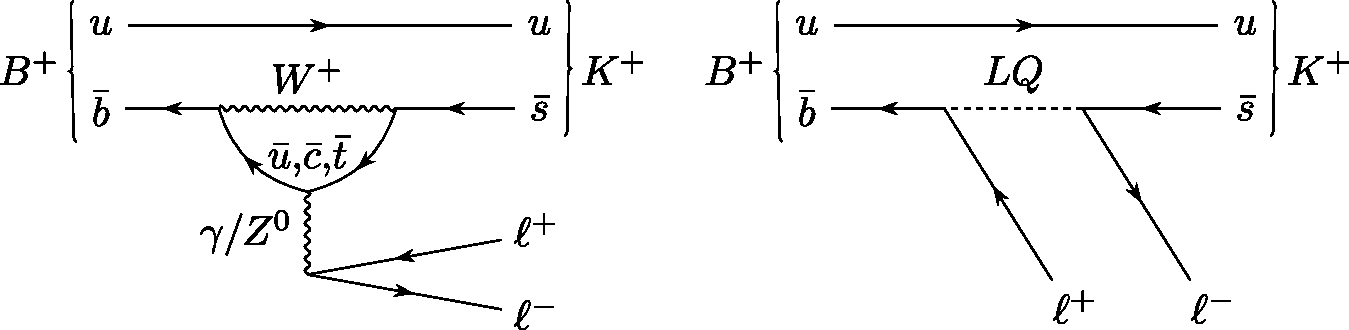
\includegraphics[width=0.96\linewidth]{figures/Fig1.pdf}
   \end{center}
   \vspace*{-0.5cm}
   \caption{
  Fundamental processes contributing to \BuKll decays in the SM and possible new physics models. A \Bp meson, consisting of \bquarkbar and \uquark quarks, decays into a \Kp, containing \squarkbar and \uquark quarks, and two charged leptons, $\ellp\ellm$. (Left) The SM contribution involves the electroweak bosons $\gamma,~W^+$ and $Z^0$. (Right) A possible new physics contribution to the decay with a hypothetical leptoquark ($LQ$) which, unlike the electroweak bosons, could have different interaction strengths with the different types of leptons.     
   }\label{fig:feyn}
\end{figure}

A distinctive feature of the SM is that the different leptons, electron ($\en$), muon ($\mun$) and tau ($\taum$),
 have the same interaction strengths. This is known as ‘lepton universality’. The only exception to this is due to the Higgs field, since the lepton-Higgs interaction strength gives rise to the differing lepton masses $m_{\tau}>m_{\mu}>m_e$. 
The suppression of $\bquarkbar \to \squarkbar$ transitions is understood in terms of the fundamental symmetries on which the SM is built. Conversely, lepton universality is an accidental symmetry of the SM, which is not a consequence of any axiom of the theory. Extensions to the SM that aim to address many of its shortfalls predict new virtual particles that could contribute to $\bquarkbar \to \squarkbar$ transitions~(see Fig.~\ref{fig:feyn}, right) and could have nonuniversal interactions, hence giving branching fractions of \BuKll
 decays with different leptons that differ from the SM predictions. Whenever a process is specified in this article, the inclusion of the charge-conjugate mode is implied.


Calculation of the SM predictions for the branching fractions of \BuKmm and \BuKee decays is complicated by the strong nuclear force that binds together the quarks into hadrons, as described by quantum chromodynamics (QCD). The large interaction strengths preclude predictions of QCD effects with the perturbation techniques used to compute the electroweak force amplitudes and only approximate  calculations are presently possible. However, the strong force does not  couple directly to leptons and hence its effect on the \BuKmm and \BuKee decays is identical. The ratio between the branching fractions of these decays is therefore predicted with $\mathcal{O}(1\%)$ precision~\cite{Descotes-Genon:2015uva,Bobeth:2007,Bordone:2016gaq,EOS,Straub:2018kue,Isidori:2020acz}. 
Due to the small masses of both electrons and muons compared to that of \bquark quarks, this ratio is predicted to be close to unity, 
except where the value of the dilepton invariant mass-squared (\qsq) significantly restricts the phase space available to form the two leptons.
Similar considerations apply to decays with other $B$ hadrons, \BuzHmm and \BuzHee, where $B=\Bu$, \Bz, \Bs or \Lb; and $H$ can be \eg an excited kaon, $\Kstarz$, or a combination of particles such as a proton and charged kaon, $p\Km$. 
The ratio of branching fractions, \RH~\cite{Hiller:2003js, Wang:2003je}, is defined in the dilepton mass-squared range $q^{2}_{\rm min} < \qsq < q^{2}_{\rm max}$ as
\begin{equation}
\label{eq:rh}
\RH \equiv  \dfrac{\displaystyle\int_{q^2_\mathrm{min}}^{q^2_{\rm max}} \dfrac{\deriv\BF(\BuzHmm)}{\deriv\qsq} \deriv\qsq}{\displaystyle\int_{q^2_{\rm min}}^{q^2_{\rm max}} \dfrac{\deriv\BF(\BuzHee)}{\deriv\qsq} \deriv\qsq} ~.
\end{equation}
\noindent 
For decays with $H\!=\!\Kp$ and $H\!=\!\Kstarz$ such ratios, denoted \RK and \RKstar, respectively, have previously been measured in similar regions of \qsq~\cite{LHCb-PAPER-2019-009, LHCb-PAPER-2017-013}.
For \RK the measurements are in the region $1.1 < \qsq < 6.0 \gevgevcccc$, whereas for \RKstar the regions are \mbox{$0.045 < \qsq < 1.1 \gevgevcccc$} and $1.1 < \qsq < 6.0 \gevgevcccc$. These ratios have been determined to be 
$2.1$--$2.5$~standard deviations below their respective SM expectations~\cite{Descotes-Genon:2015uva,Bobeth:2007,Bordone:2016gaq,Capdevila:2016ivx,Capdevila:2017ert,Serra:2016ivr,EOS,Straub:2015ica,Straub:2018kue,Altmannshofer:2017fio,Jager:2014rwa}. 
The analogous ratio has also been measured for \Lb decays with $H=p\Km$ and is compatible with unity at the level of one standard deviation~\cite{LHCb-PAPER-2019-040}.

These decays all proceed via
 the same \btosbar quark transition and the results have therefore further increased interest in measurements of angular observables~\cite{LHCb-PAPER-2020-041,LHCb-PAPER-2020-002,LHCb-PAPER-2015-051,Aaboud:2018krd,Aubert:2006vb,Lees:2015ymt,Wei:2009zv,Wehle:2016yoi,Aaltonen:2011ja,Khachatryan:2015isa,Sirunyan:2017dhj} and branching fractions~\cite{LHCb-PAPER-2016-012, LHCb-PAPER-2015-023, LHCb-PAPER-2014-006, LHCb-PAPER-2015-009} of decays mediated by \btosmumubar transitions. Such decays also exhibit some tension with the SM predictions but the extent of residual QCD effects is still the subject of debate~\cite{Jager:2014rwa, Descotes-Genon:2015uva,Lyon:2014hpa,Khodjamirian:2012rm,Khodjamirian:2010vf,Descotes-Genon:2014uoa,Horgan:2013pva, Beaujean:2013soa, Hambrock:2013zya, Altmannshofer:2013foa,Bobeth:2017vxj}.
A consistent model-independent interpretation of all these data is possible via a modification of the \mbox{$\bquarkbar \to \squarkbar$} coupling strength~\cite{Ciuchini:2020gvn,Kowalska:2019ley,Alguero:2019ptt,Hurth:2020rzx,Ciuchini:2019usw,Aebischer:2019mlg,Alok:2019ufo}. 
Such a modification can be realised in new physics models with an additional heavy neutral boson~\cite{Altmannshofer:2014cfa, Crivellin:2015mga, Celis:2015ara, Falkowski:2015zwa,Allanach:2019mfl,Allanach:2019iiy,Kawamura:2019rth,Dwivedi:2019uqd,Han:2019diw,Capdevila:2020rrl,Altmannshofer:2019xda,Chen:2020szf,Carvunis:2020exc,Karozas:2020zvv,Borah:2020swo,Allanach:2020kss,Sheng:2021tom} or with leptoquarks~\cite{Hiller:2014yaa,Gripaios:2014tna,Varzielas:2015iva,Barbieri:2016las,Bordone2018,Fornal:2018dqn,Balaji:2019kwe,Cornella:2019hct,Datta:2019tuj,Popov:2019tyc,Bigaran:2019bqv,Bernigaud:2019bfy,DaRold:2019fiw,Fuentes-Martin:2019bue,Hati:2019ufv,Datta:2019bzu,Crivellin:2019dwb,Borschensky:2020hot,Saad:2020ihm,Fuentes-Martin:2020bnh,Dev:2020qet,Fornal:2020ngq,Davighi:2020qqa}. Other explanations of the data involve a variety of extensions to the SM, such as supersymmetry, extended Higgs-boson sectors and models with extra dimensions~\cite{Barman:2018jhz,Shaw:2019fin,Arnan:2019uhr,Trifinopoulos:2019lyo,DelleRose:2019ukt,Ordell:2019zws,Marzo:2019ldg,Darme:2020hpo,Hu:2019ahp,Hu:2020yvs}.
Tension with the SM is also seen in the combination of several ratios that test lepton-universality in \btoclnubar transitions~\cite{Lees:2012xj,LHCb-PAPER-2017-035,Lees:2013uzd,Sato:2016svk,LHCb-PAPER-2015-025,Huschle:2015rga,LHCb-PAPER-2017-027,Belle:2019rba,Hirose:2017dxl}. 
 
In this article, a measurement of the \RK ratio is presented based on proton-proton collision data collected with the LHCb detector at CERN’s Large Hadron Collider (see Methods). The data were recorded during the years 2011, 2012 and 2015--2018, in which the centre-of-mass energy of the collisions was $7$, $8$ and $13\tev$, and correspond to an integrated luminosity of 9\invfb. Compared to the previous LHCb \RK result~\cite{LHCb-PAPER-2019-009}, the experimental method is essentially identical but the analysis uses an additional $4\invfb$ of data collected in 2017 and 2018. The results supersede those of the previous \lhcb analysis. 

The analysis strategy aims to reduce systematic uncertainties induced in modelling the markedly different reconstruction of decays with muons in the final state, compared to decays with electrons. These differences arise due to the significant bremsstrahlung radiation emitted by the electrons and the different detector subsystems that are used to identify electron and muon candidates (see Methods). The major challenge of the measurement is then correcting for the efficiency of the selection requirements used to isolate signal candidates and reduce background. In order to avoid unconscious bias, the analysis procedure was developed and the cross-checks described below performed before the result for \RK was examined. 

In addition to the process discussed above, the \Kll final state is produced via a $\Bp \to X_{\quark\quarkbar}\Kp$ decay, where $X_{\quark\quarkbar}$ is a bound state (meson) such as the \jpsi. The \jpsi meson consists of a charm quark and antiquark, \cquark\cquarkbar, and is produced resonantly at $\qsq=9.59\gevgevcccc$. This ‘charmonium’ resonance subsequently decays into two leptons, \Jpsill. The \BuJpsiKll decays are not suppressed and hence have a branching fraction 
orders of magnitude larger than that of \BuKll decays.
These two processes are separated by applying a requirement on \qsq. The $1.1 < \qsq < 6.0 \gevgevcccc$ region used to select \BuKll decays is chosen to reduce the pollution from the \jpsi resonance and the high-\qsq region that contains contributions from further excited charmonium resonances, such as the \psitwos and \psiprpr states, and from lighter $\squark\squarkbar$ resonances, such as the $\phi(1020)$ meson. In the remainder of this article, the notation \BuKll is used to denote only decays with \mbox{$1.1<\qsq<6.0\gevgevcccc$}, which are referred to as nonresonant, whereas \BuJpsiKll decays are denoted resonant.


To help overcome the challenge of modelling precisely the different electron and muon reconstruction efficiencies, the branching fractions of \BuKll decays are measured relative to those of \BuJpsiK decays~\cite{LHCb-PAPER-2014-024}. Since the $\jpsi\to\ell^+\ell^-$ branching fractions are known to respect lepton universality to within 0.4\%~\cite{Ablikim:2013pqa,PDG2020}, the \RK ratio is determined via the double ratio of branching fractions
    \begin{equation}
    \label{eq:doubleratio}
       \RK = {\frac{\BR(\BuKmm)}{\BR(\BuJpsiKmm)}} \bigg{/} {\frac{\BR(\BuKee)}{\BR(\BuJpsiKee)}} \, .
    \end{equation}
\noindent In this equation, each branching fraction can be replaced by the corresponding event yield divided by the appropriate overall detection efficiency (see Methods), as all other factors needed to determine each branching fraction individually cancel out. 
The efficiency of the nonresonant \BuKee decay therefore needs to be known only relative to that of the resonant \BuJpsiKee decay, rather than relative to the \BuKmm decay. 
As the detector signature of each resonant decay is similar to that of its corresponding nonresonant decay, systematic uncertainties that would otherwise dominate the calculation of these efficiencies are suppressed. The yields observed in these four decay modes and the ratios of efficiencies determined from simulated events then enable an \RK measurement with statistically dominated uncertainties. Percent-level control of the efficiencies is verified with a direct comparison of the \BuJpsiKee and \BuJpsiKmm branching fractions in the ratio \mbox{$\rjpsi=\BR(\BuJpsiKmm)/\BR(\BuJpsiKee)$}, as detailed below. 

Candidate \BuKll decays are found by combining the reconstructed trajectory~(track) of a particle identified as a charged kaon, together with the tracks from a pair of well-reconstructed oppositely charged particles identified as either electrons or muons. The particles are required to originate from a common vertex, displaced from the proton-proton interaction point, with good vertex-fit quality. The techniques used to identify the different particles and to form \Bp candidates are described in Methods. 


The invariant mass of the final state particles, \mKll, is used to discriminate between signal and background contributions, with the signal expected to accumulate around the known mass of the \Bp meson.
Background originates from particles selected from multiple hadron decays, referred to as combinatorial background, and from the specific decays of $B$-hadrons. 
The latter also tend to accumulate around specific values of \mKll.
For the muon modes, the residual background is combinatorial and, for the resonant mode, there is an additional contribution from \BuJpsipi decays with a pion misidentified as a kaon. 
For the electron modes, in addition to combinatorial background, other specific background decays contribute significantly in the signal region. The dominant such background for the nonresonant and resonant modes come from partially reconstructed \BuBdKpiplusee and \BuBdKpijpsi decays, respectively, where the pion is not included in the \Bp candidate. Decays of the form \BuDzenu also contribute at the level of $\mathcal{O}(1\%)$ of the \BuKee signal; and there is also a contribution from \BuJpsiKee decays, where a photon is emitted but not reconstructed. 
The kinematic correlation between \mKee and {\qsq} means that, irrespective of misreconstruction effects, the latter background can only populate the \mKee region well below the signal peak. 

\begin{figure}[!t]
    \centering
    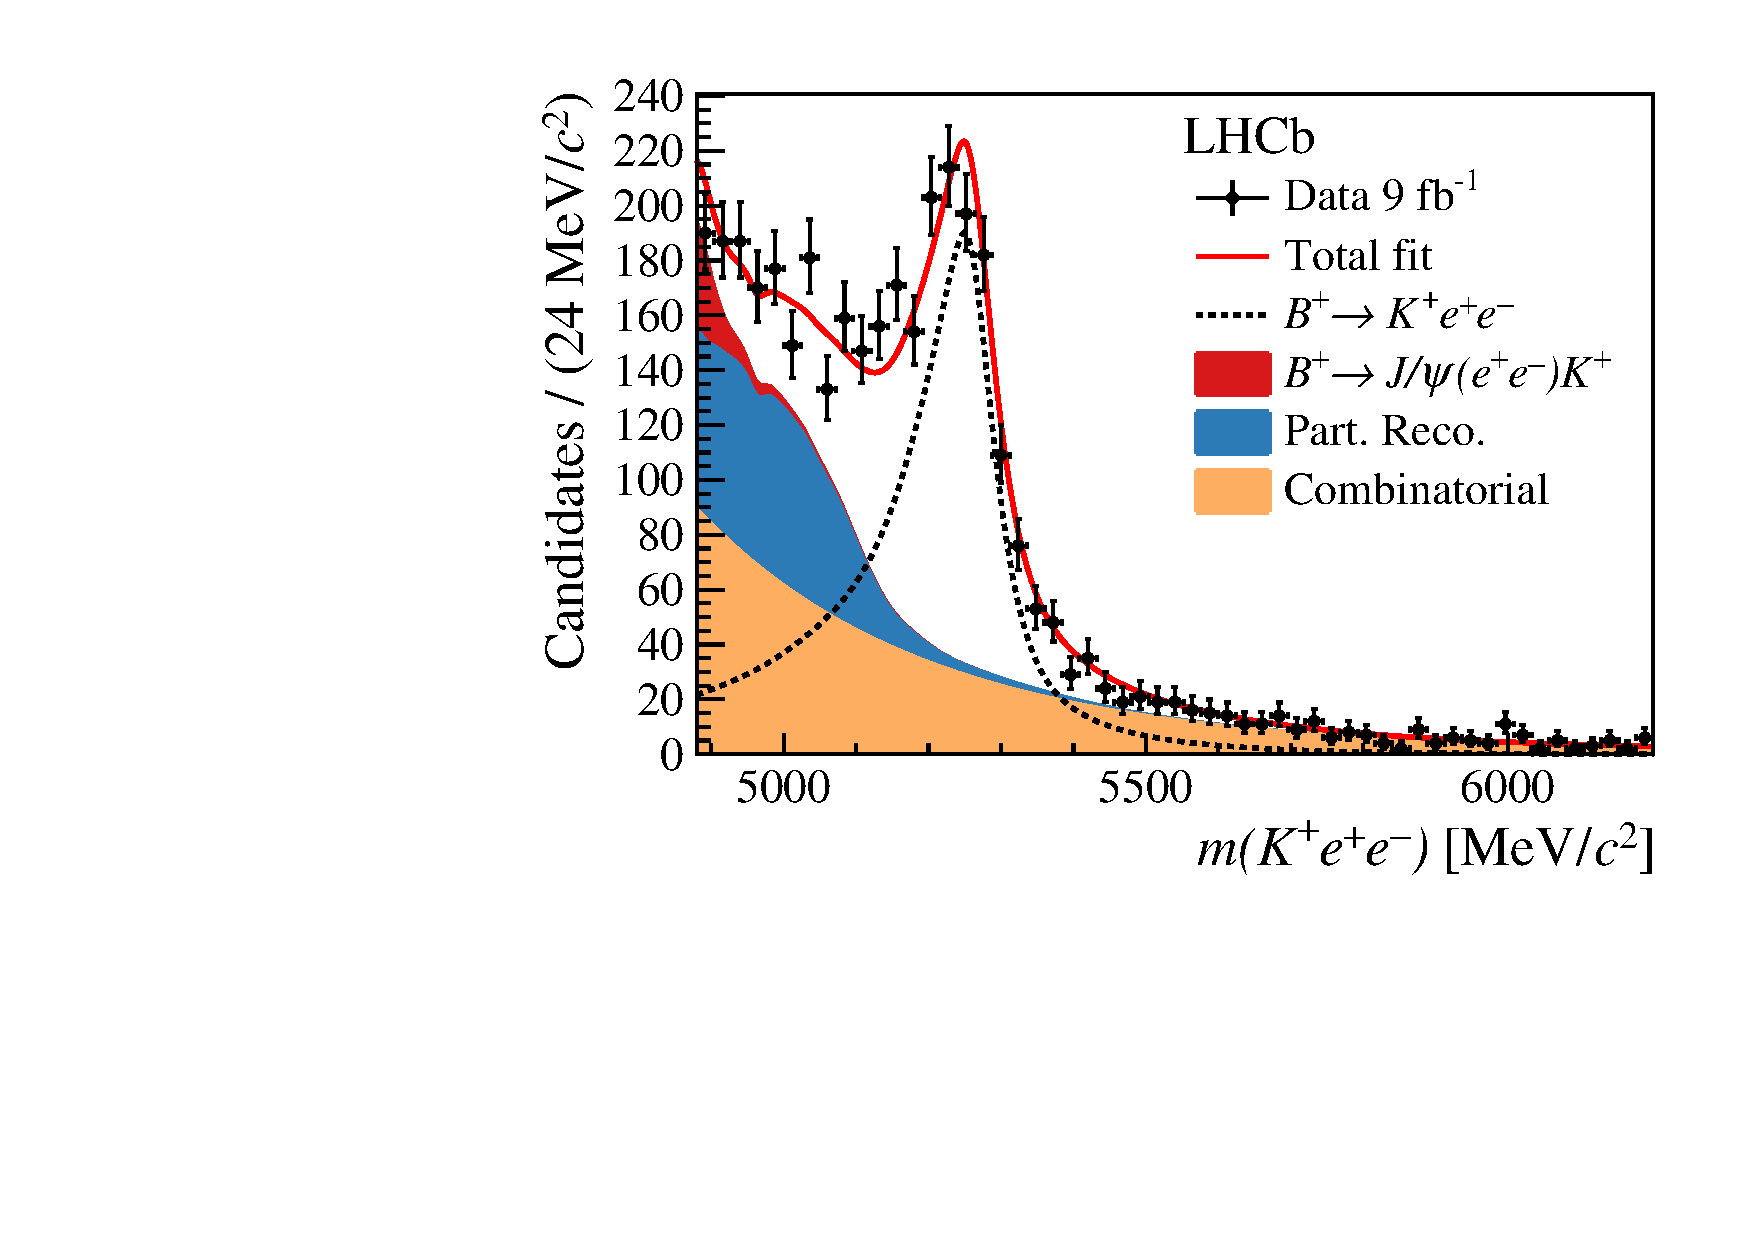
\includegraphics[width=0.45\textwidth]{figures/Fig2a.pdf}
    %plotKeeDataFitRunAllTrigAll.pdf}
    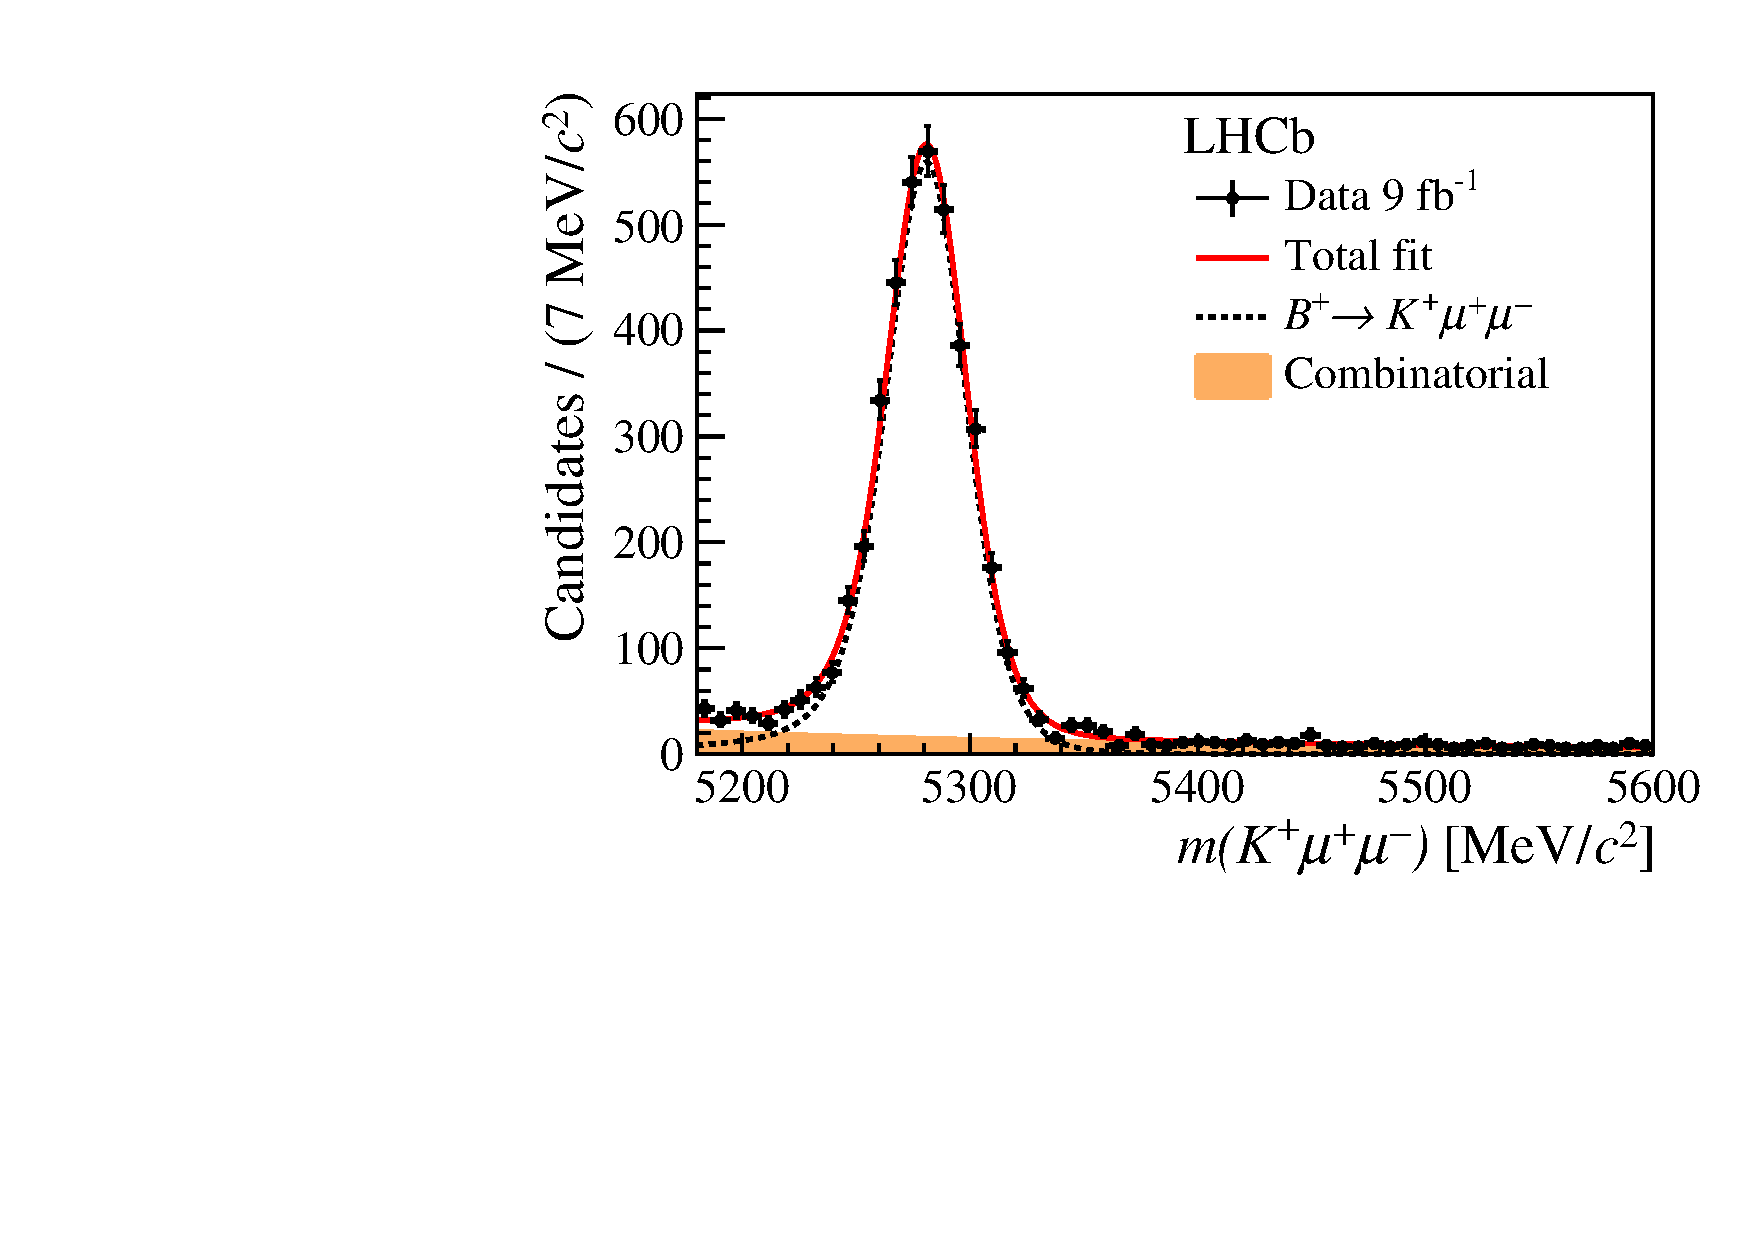
\includegraphics[width=0.45\textwidth]{figures/Fig2b.pdf}
    %plotKmumuDataFitRunAll.pdf}
    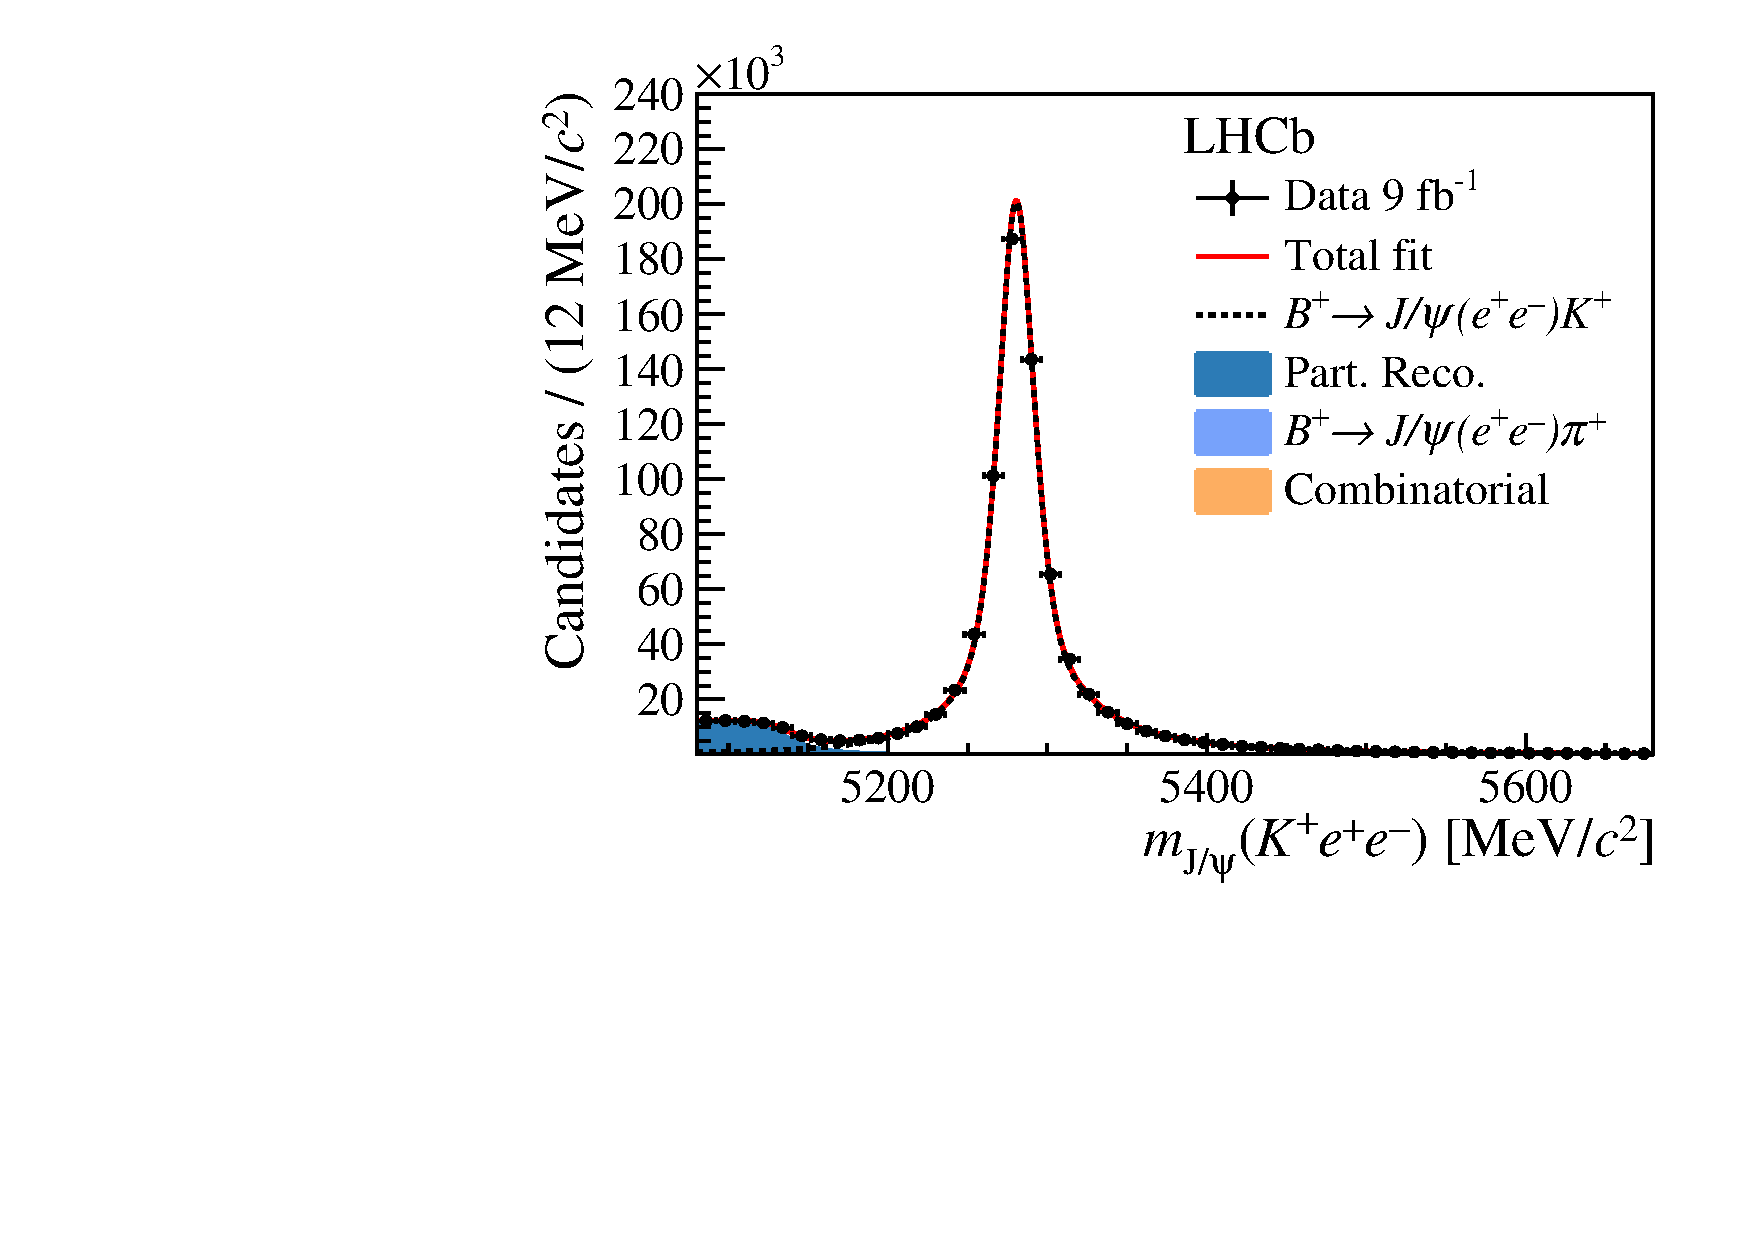
\includegraphics[width=0.45\textwidth]{figures/Fig2c.pdf}
    %plotKJpsieeDataFitTrig-1All.pdf}
    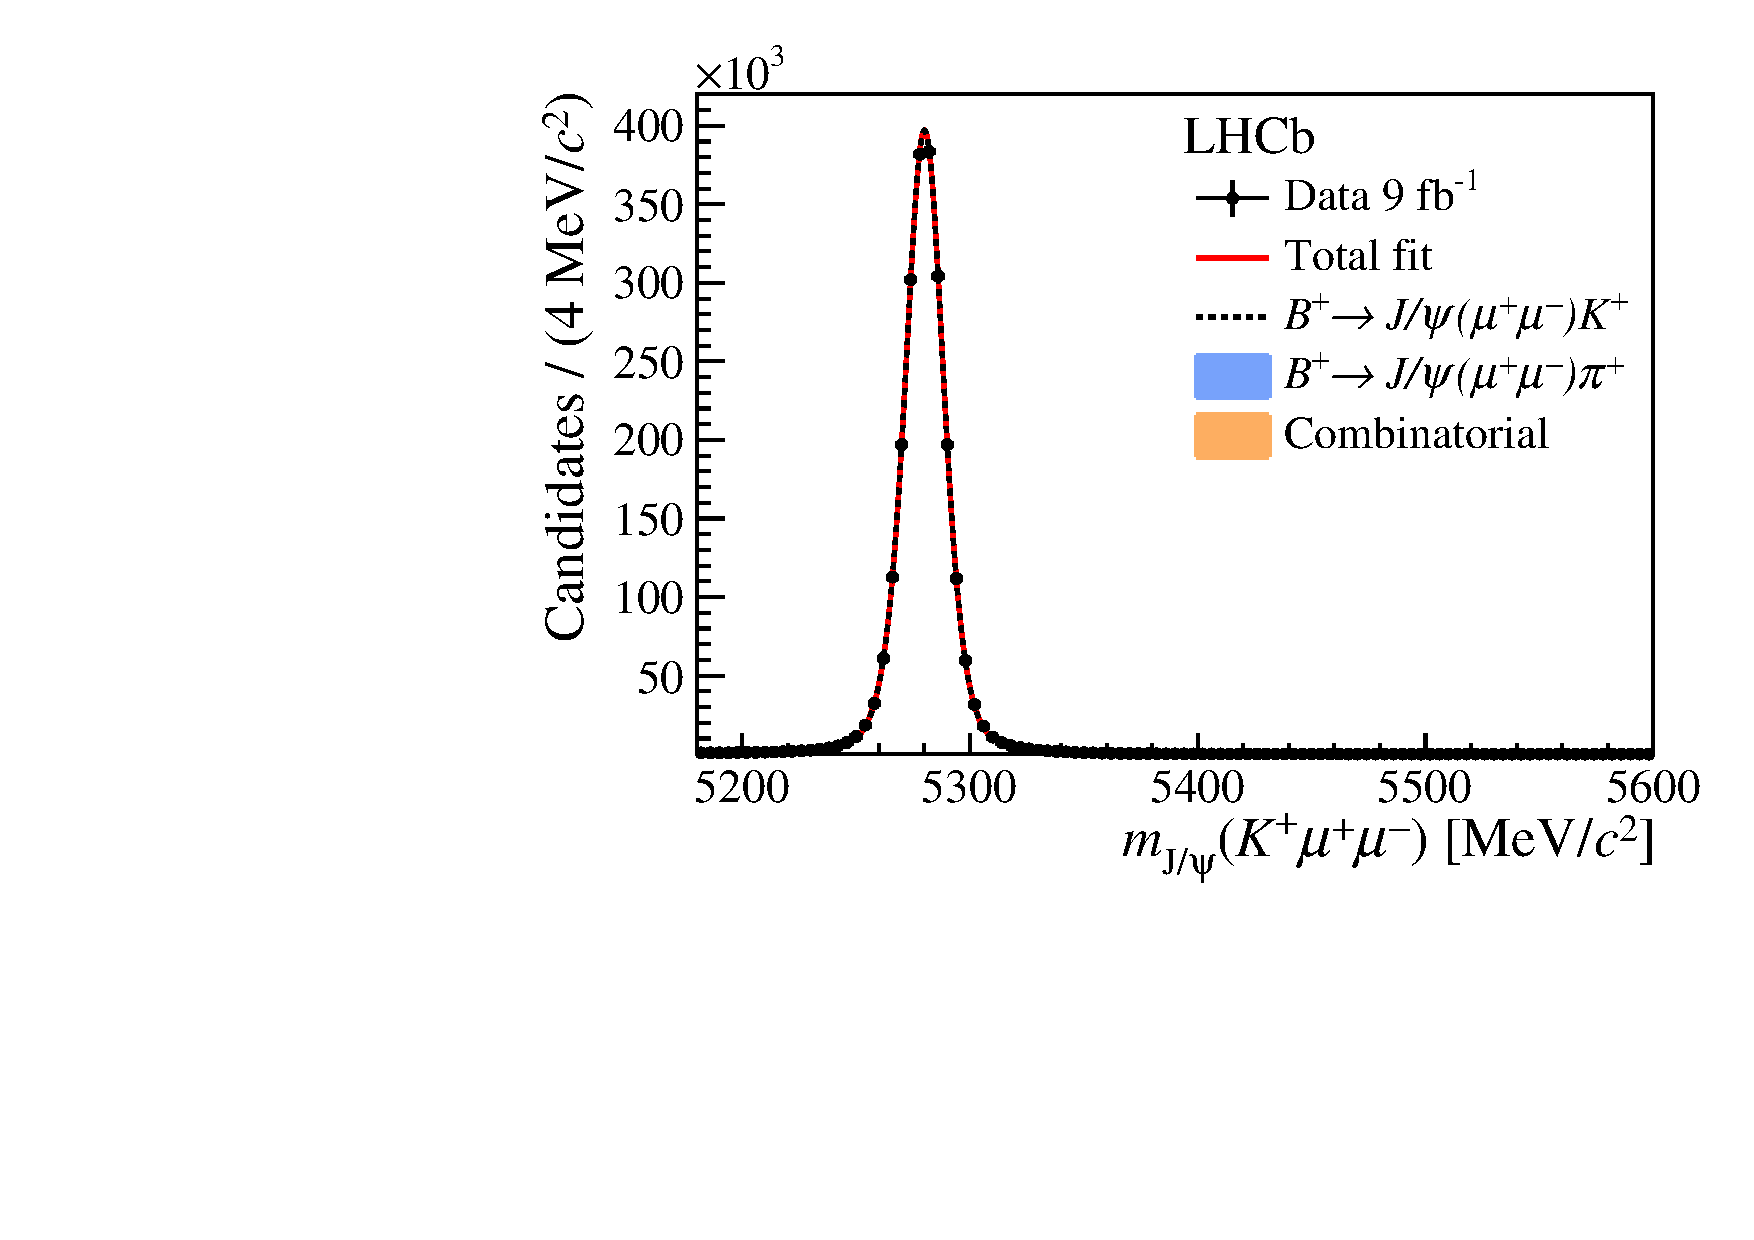
\includegraphics[width=0.45\textwidth]{figures/Fig2d.pdf}
    %plotKJpsimumuDataFitAll.pdf}
    \caption{Candidate invariant mass distributions. Distribution of the invariant mass \mKllgeneric for candidates with (left) electron and (right) muon pairs in the final state for the (top) nonresonant \BuKll signal channels and (bottom) resonant \BuJpsiKll decays. The fit projection is superimposed. In the resonant-mode distributions, some fit components are too small to be visible.
    }
    \label{fig:fits}
\end{figure}



After the application of the selection requirements, the resonant and nonresonant decays are clearly visible in the mass distributions (see Fig.~\ref{fig:fits}). The yields  in the two \BuKll and two \BuJpsiKll decay modes are determined by performing unbinned extended maximum-likelihood fits to these distributions (see Methods). 
For the nonresonant candidates, the \mKee and \mKmm distributions are fitted with a likelihood function that has the \BuKmm yield and \RK as fit parameters and the resonant decay-mode yields incorporated as Gaussian-constraint terms.
The resonant yields are determined from separate fits
to the mass, \mKllconst, formed by kinematically constraining the dilepton system to the known \jpsi mass~\cite{PDG2020} and thereby improving the mass resolution.



Simulated events are used to derive the two ratios of efficiencies needed to form \RK using Eq.~\eqref{eq:doubleratio}. Control channels are used to calibrate the simulation in order to correct for the imperfect modelling of the \Bu production kinematics and various aspects of the detector response. The overall effect of these corrections on the measured value of \RK is a relative shift of $(+3\pm1)\%$.
When compared with the 20\% shift that these corrections induce in the measurement of \rjpsi, this demonstrates the robustness of the double-ratio method in suppressing systematic biases that affect the resonant and nonresonant decay modes similarly.

The systematic uncertainty (see Methods) from the choice of signal and background mass-shape models in the fits is estimated by fitting pseudoexperiments with alternative models that still describe the data well. The effect on \RK is at the $1\%$ level. A  comparable uncertainty arises from the limited size of the calibration samples, with negligible contributions from the calibration of the \Bu production kinematics and modelling of the selection and particle-identification efficiencies. Systematic uncertainties that affect the ratios of efficiencies influence the measured value of \RK and are taken into account using constraints on the efficiency values. Correlations between different categories of selected events and data-taking periods are taken into account in these constraints. The combined statistical and systematic uncertainty is then determined by scanning the profile-likelihood and the statistical contribution to the uncertainty is isolated by repeating the scan with the efficiencies fixed to their fitted values.  

The determination of the \rjpsi ratio requires control of the relative selection efficiencies for the resonant electron and muon modes, and does not therefore benefit from the cancellation of systematic effects in the double ratio used to measure \RK. Given the scale of the corrections required, comparison of \rjpsi with unity is a stringent cross check of the experimental procedure. 
In addition, if the simulation is correctly calibrated, the measured \rjpsi value will not depend on any variable.
This ratio is therefore also computed as a function of different kinematic variables that are chosen to provide overlap with the spectra of the nonresonant decays. Although the range of \qsq differs between resonant and nonresonant decays, the efficiency depends on laboratory-frame variables such as the momenta of the final-state particles, or the opening angle between the two leptons, rather than directly on \qsq. A given set of values for the final-state particles' momenta and angles in the \Bp rest frame will result in a distribution of such values when transformed to the laboratory frame. As a result, there is significant overlap between the nonresonant and resonant samples in the relevant distributions, even if they are mutually exclusive as a function of \qsq. 

The value of \rjpsi is measured to be $0.981\pm0.020$, where the uncertainty includes both statistical and systematic effects.
The consistency of this ratio with unity demonstrates control of the efficiencies well in excess of that needed for the determination of \RK. 
In the measurement of the \rjpsi ratio, the systematic uncertainty is dominated by the imperfect modelling of the \Bu production kinematics and the modelling of selection requirements, which have a negligible impact on the \RK measurement.
No significant trend is observed in the differential determination of \rjpsi as a function of any considered variable. An example distribution, with \rjpsi determined as a function of \Bp momentum component transverse to the beam direction, \pt, is shown in Fig.~\ref{fig:rjpsi_differential}. Assuming the observed \rjpsi variation in such distributions reflects genuine mismodelling of the efficiencies, rather than statistical fluctuations, and taking into account the spectrum of the relevant variables in the nonresonant decay modes, a total shift on \RK is computed for each of the variables examined. In each case, the resulting variation is within the estimated systematic uncertainty on \RK. Similarly, double differential
computations of the \rjpsi ratio also do not show any trend and are consistent with the systematic uncertainties assigned on the \RK measurement.

\begin{figure}[!b]
   \begin{center}

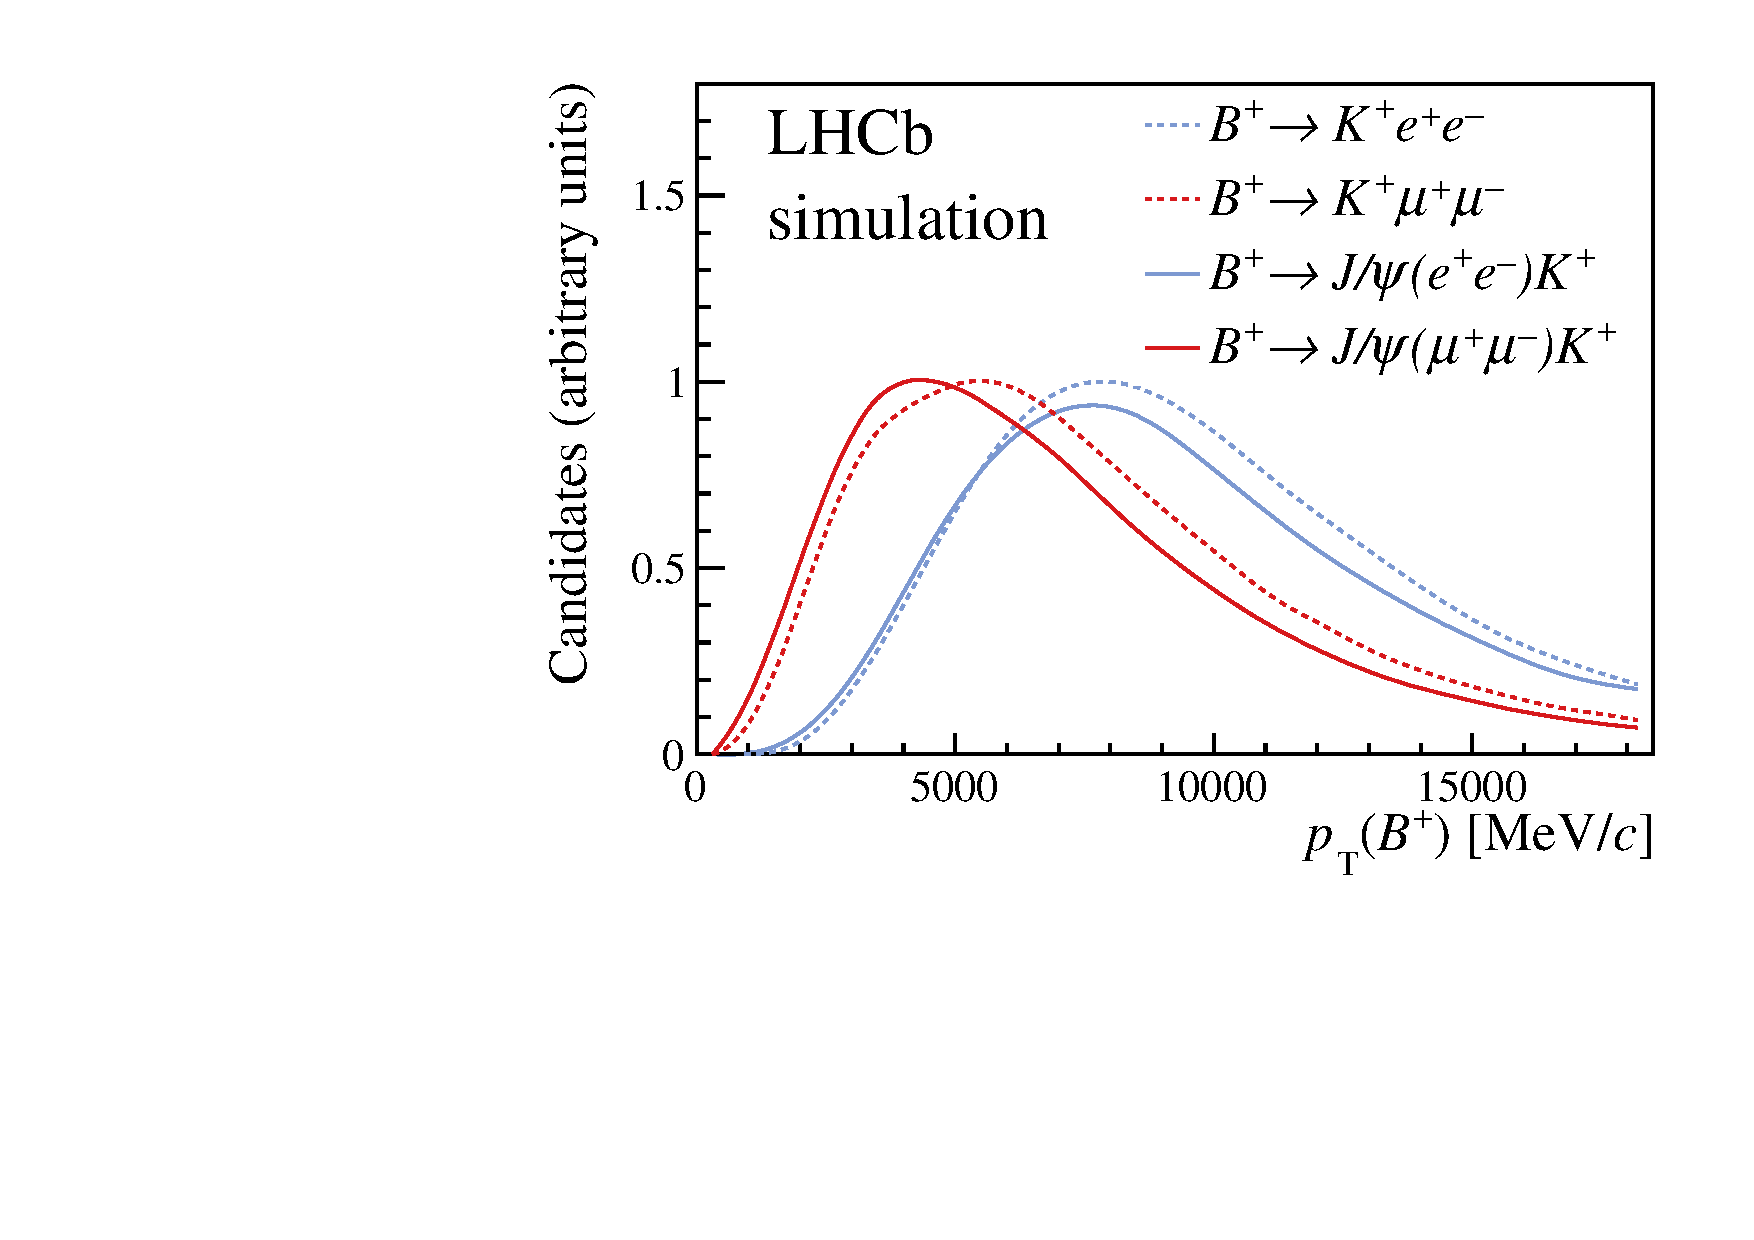
\includegraphics[width=0.45\linewidth,trim={0 0 0 0.5cm}, clip]{figures/Fig3a.pdf}
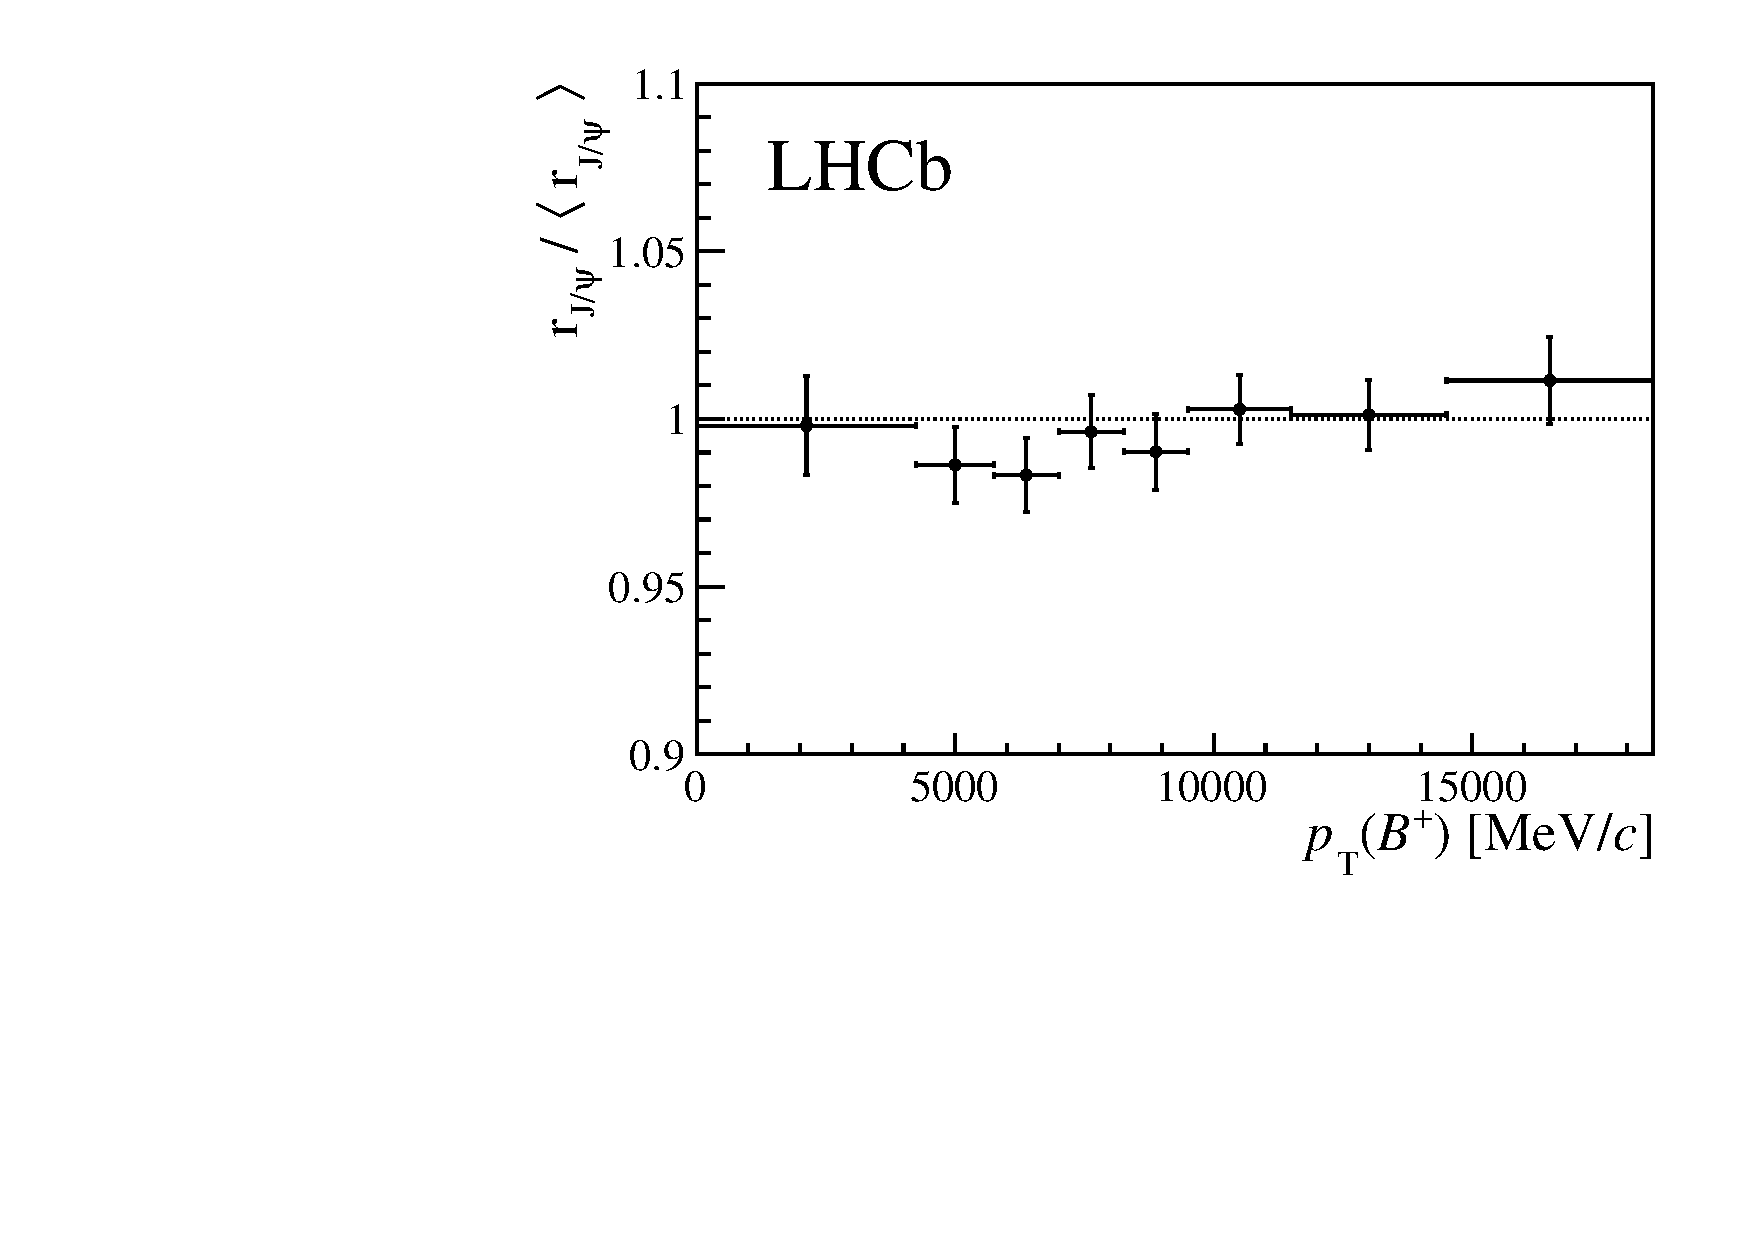
\includegraphics[width=0.45\linewidth,trim={0 0.15cm 0 0}, clip]{figures/Fig3b.pdf}
      \end{center}
      \caption{Differential \rjpsi measurement. The 
      distributions of (left) the \Bp transverse momentum, \pt, and (right) the ratio \rjpsi relative to its average value $\left< \rjpsi \right>$ as a function of \pt. The distribution from the \BuJpsiK decays is similar to that of the corresponding \BuKll decays such that the measurement of \rjpsi tests the kinematic region relevant for the \RK measurement. The lack of any dependence of the value of $\rjpsi/\left< \rjpsi \right>$ as a function of \Bp $p_{\mathrm T}$ demonstrates control of the efficiencies.}
    \label{fig:rjpsi_differential}
\end{figure}

In addition to \BuJpsiK decays, 
clear signals are observed from \BuPsiK decays. 
The double ratio of branching fractions, \RPsitwos, defined by
\begin{equation}
\label{eq:RPsitwos}
\RPsitwos  =
{\frac{\BR(\BuPsiKmm)}{\BR(\BuJpsiKmm)}} \bigg{/} {\frac{\BR(\BuPsiKee)}{\BR(\BuJpsiKee)}}  \,,
\end{equation}
\noindent provides an independent validation of the double-ratio analysis procedure and further tests the control of the efficiencies. 
This double ratio is expected to be close to unity~\cite{PDG2020}
and is determined to be $0.997\pm 0.011$, where the uncertainty includes both statistical and systematic effects.
This can be interpreted as a world-leading test of lepton flavour universality in $\psi(2S) \rightarrow \ell^+\ell^-$ decays.

The fit projections for the \mKll and \mKllconst distributions are shown in Fig.~\ref{fig:fits}. The fit is of good quality and the value of \RK is measured to be
\begin{displaymath}
\RK (1.1 < \qsq < 6.0 \gevgevcccc) = \RKvalue\,,
\end{displaymath}
\noindent where the first uncertainty is statistical and the second systematic. Combining the uncertainties gives $\RK=\RKvalueComb$.
This is the most precise measurement to date and is consistent with the SM expectation, \mbox{$1.00 \pm 0.01$}~\cite{Descotes-Genon:2015uva,Bobeth:2007,Bordone:2016gaq,EOS,Straub:2018kue}, at the level of 0.10\% (\significance~standard deviations), giving evidence for the violation of lepton universality in these decays.
The value of \RK is found to be consistent in subsets of the data divided on the basis of data-taking period, selection category and magnet polarity (see Methods).
The profile-likelihood is given in Methods. A comparison with previous measurements is shown in Fig.~\ref{fig:RKresult}.

The $3850\pm 70$ \BuKmm decay candidates that are observed are used to compute the \BuKmm  branching fraction as a function of \qsq. The results are consistent between the different data-taking periods and with previous \lhcb measurements~\cite{LHCb-PAPER-2014-006}.
The \BuKee branching fraction is determined by combining the value of \RK with the value of $\deriv\BR(\BuKmm)/\deriv\qsq$ in the region $(1.1 < \qsq < 6.0 \gevgevcccc)$~\cite{LHCb-PAPER-2014-006}, taking into account correlated systematic uncertainties. This gives
\begin{displaymath}
\frac{\deriv\BR(\BuKee)}{\deriv\qsq}(1.1 < \qsq < 6.0 \gevgevcccc)  = (28.6\,^{+\, 1.5}_{-\, 1.4} \,\pm 1.3)\times 10^{-9}\,c^4\kern -0.1em/\kern -0.15em\gev^2\,.
\end{displaymath}
\noindent The limited knowledge of the \BuJpsiK branching fraction~\cite{PDG2020} gives rise to the dominant systematic uncertainty. This is the most precise measurement of this quantity to date and, given the large theoretical uncertainty on the predictions~\cite{Khodjamirian:2017fxg,Straub:2018kue}, is consistent with the SM.


A breaking of lepton universality would require an extension of the gauge structure of the SM that gives rise to the known fundamental forces. It would therefore constitute a significant evolution in our understanding and would challenge an inference based on a wealth of experimental data in other processes. Confirmation of any beyond the SM effect will clearly require independent evidence from a wide range of sources.

\begin{figure}[!t]
    \centering
    %RK2021_column
    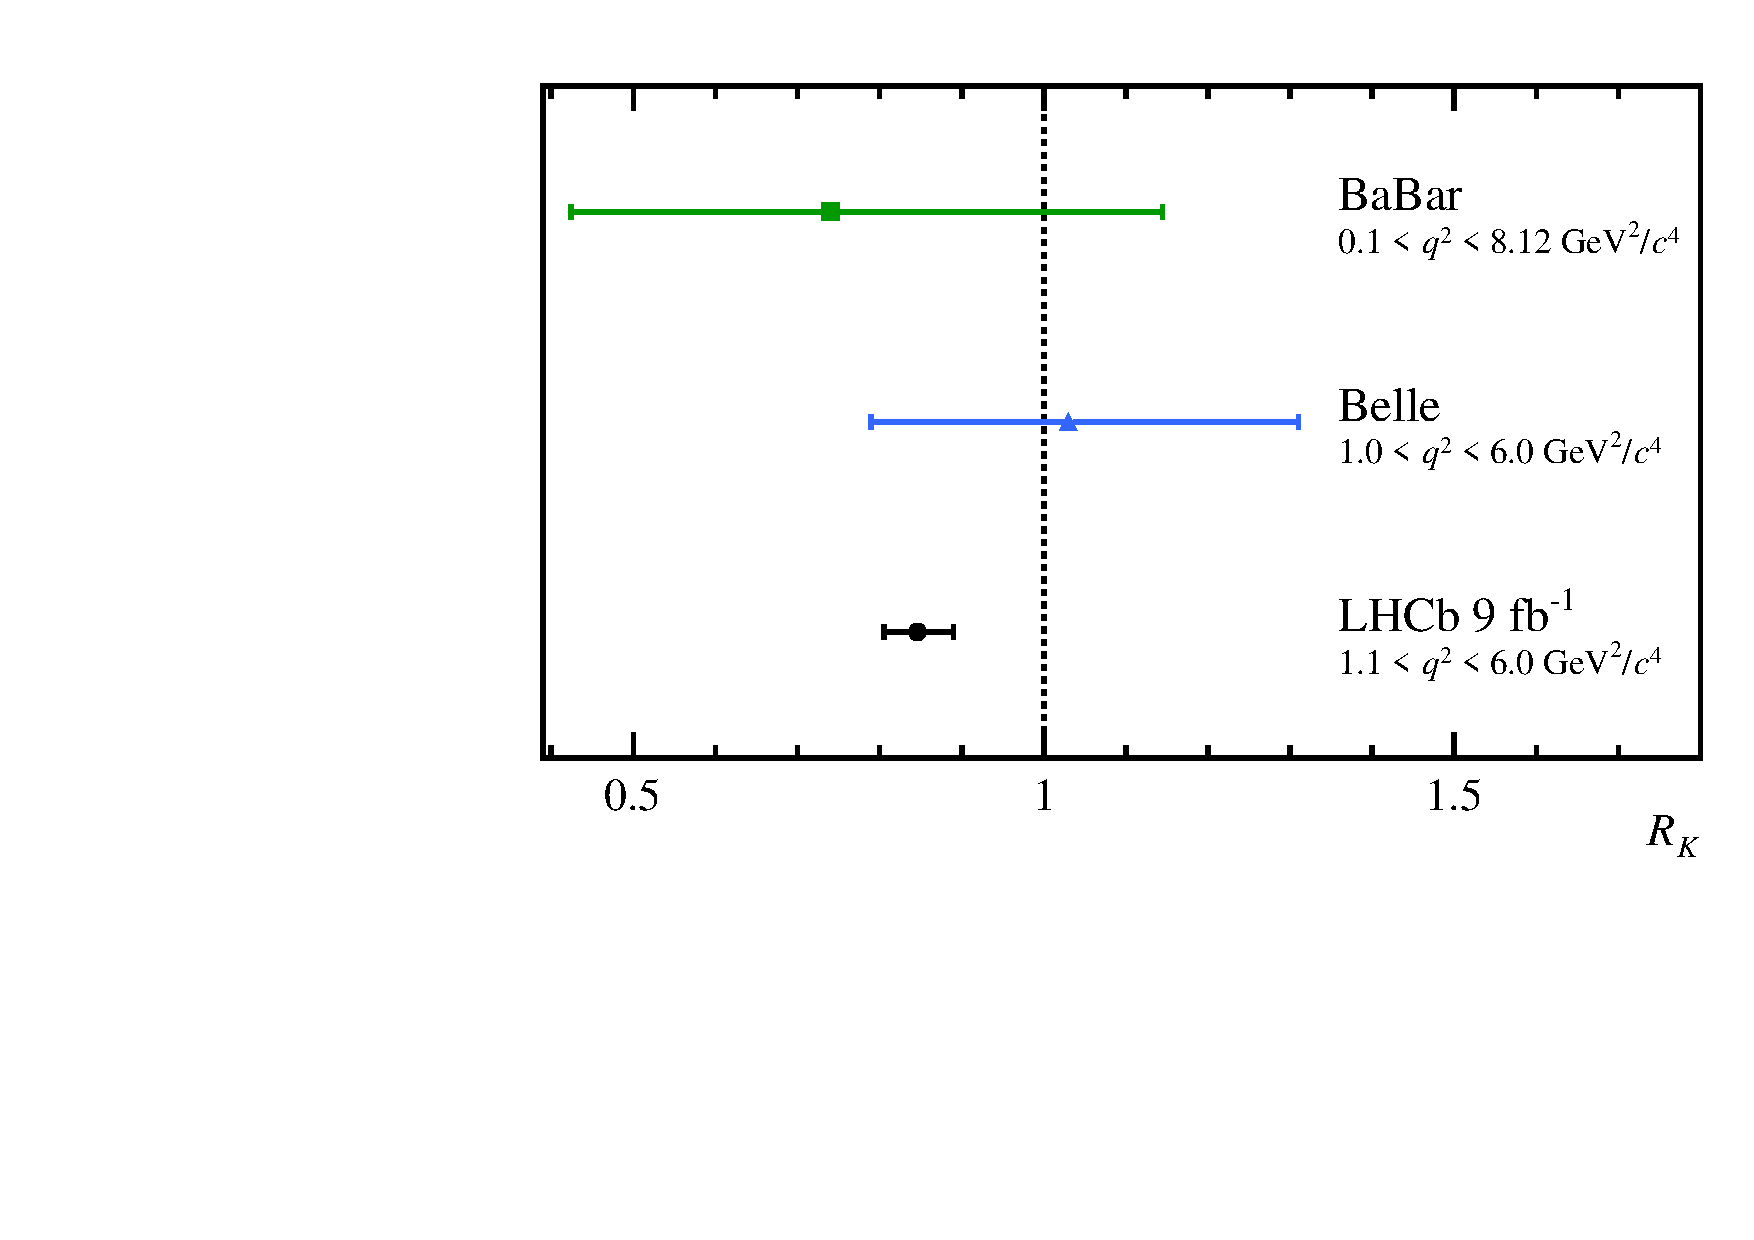
\includegraphics[width=0.7\textwidth]{figures/Fig4.pdf} 
    \caption{Comparison between \RK measurements. 
    In addition to the LHCb result, the measurements by the BaBar~\cite{RKbabar} and Belle~\cite{RKbelle} collaborations, which combine \BuKll and \BdKSll decays, are also shown.
    }
    \label{fig:RKresult}
\end{figure}

Measurements of other $R_H$ observables with the full LHCb data set will provide further information on the quark-level processes measured. 
In addition to affecting the decay rates, new physics can also alter how the decay products are distributed in phase space. 
An angular analysis of the electron mode, where SM-like behaviour might be expected in the light of the present results and those from \btosmumubar decays, would allow the formation of ratios between observable quantities other than branching fractions, enabling further precise tests of lepton universality~\cite{Altmannshofer:2015mqa,Capdevila:2016ivx,Wehle:2016yoi,Geng:2017svp,Serra:2016ivr}. The hierarchical effect needed to explain the existing \bsllbar and \btoclnubar data, with the largest effects observed in tau modes, then muon modes, and little or no effects in electron modes, suggests that studies of \btostautaubar transitions are also of great interest~\cite{LHCb-PAPER-2017-003, TheBaBar:2016xwe}. There are excellent prospects for all of the above and further measurements with the much larger samples that will be collected with the upgraded LHCb detector from 2022 and, in the longer term, with the LHCb Upgrade~II~\cite{LHCb-PII-Physics}. Other experiments should also be able to determine $R_H$ ratios, with the Belle II experiment in particular expected to have competitive sensitivity~\cite{Kou:2018nap}.

In summary, in the dilepton mass-squared region $1.1 < \qsq < 6.0 \gevgevcccc$, the ratio of branching fractions for \BuKmm and \BuKee decays is measured to be $\RK=\RKvalueComb$. 
This is the most precise measurement of this ratio to date and is compatible with the SM prediction with a p-value of 0.10\%. The significance of this discrepancy is \significance standard deviations, giving evidence for the violation of lepton universality in these decays.

\newpage
\section*{Methods}
\subsection*{Experimental setup}

The Large Hadron Collider (LHC) is the world’s highest-energy particle accelerator and is situated approximately 100\,m underground, close to Geneva, Switzerland. The collider accelerates two counter-rotating beams of protons, guided by superconducting magnets located around a 27\,km circular tunnel, and brings them into collision at four interaction points that house large detectors. The LHCb experiment~\cite{Alves:2008zz,LHCb-DP-2014-002} is instrumented in the region covering the polar angles between 10 and 250\,mrad around the proton beam axis, in which the products from $B$-hadron decays can be efficiently captured and identified. The detector includes a high-precision tracking system with a dipole magnet, providing measurements of momentum and impact parameter (IP), defined for charged particles as the minimum distance of a track to a primary proton-proton interaction vertex (PV). Different types of charged particles are distinguished using information from two ring-imaging Cherenkov (RICH) detectors, a calorimeter and a muon system~\cite{LHCb-DP-2014-002, LHCb-DP-2014-001, LHCb-DP-2013-003,LHCb-DP-2013-001,LHCb-DP-2012-003,LHCb-DP-2012-002}. 

Since the associated data storage and analysis costs would be prohibitive, the experiment does not record all collisions. 
Only potentially interesting events, selected using real-time event filters referred to as triggers, are recorded.
% Instead, a subset of interesting events are isolated for further study using real-time event filters known as triggers. 
The LHCb trigger system has a hardware stage, based on information from the calorimeter and muon systems; followed by a software stage that uses all the information from the detector, including the tracking, to make the final selection of events to be recorded for subsequent analysis. The trigger selection algorithms are based on identifying key characteristics of $B$ hadrons and their decay products, such as high \pt final state particles, and a decay vertex that is significantly displaced from any of the PVs in the event.

For the \RK measurement, candidate events are  required to have passed a hardware trigger algorithm that selects either a high \pt muon; or an electron, hadron or photon with high transverse energy deposited in the calorimeters. The \BuKmm and \BuJpsiKmm candidates must be triggered by one of the muons, whereas \BuKee and \BuJpsiKee candidates must be triggered in one of three ways: by either one of the electrons; by the kaon from the \Bp decay; or by particles in the event that are not decay products of the \Bp candidate. In the software trigger, the tracks of the final-state particles are required to form a displaced vertex with good fit quality. A multivariate algorithm is used for the identification of displaced vertices consistent with the decay of a $B$ hadron~\cite{BBDT, LHCb-PROC-2015-018}.

\subsection*{Analysis description}

The analysis technique used to obtain the results presented in this article is essentially identical to that used to obtain the previous LHCb \RK measurement, described in Ref.~\cite{LHCb-PAPER-2019-009} and only the main analysis steps are reviewed here. 

\subsubsection*{Event selection} 

Kaon and muon candidates are identified using the output of multivariate classifiers that exploit information from the tracking system, the RICH detectors, the calorimeters and the muon chambers.
Electrons are identified by matching tracks to  particle showers in the electromagnetic calorimeter~(ECAL) and using the ratio of the energy detected in the ECAL to the momentum measured by the tracking system. 
An electron that emits a bremsstrahlung photon due to interactions with the material of the detector downstream of the dipole magnet results in the photon and electron depositing their energy in the same ECAL cells, and therefore in a correct measurement of the original energy of the electron in the ECAL. However, a bremsstrahlung photon emitted upstream of the magnet  will deposit energy in a different part of the ECAL than the electron, which is deflected in the magnetic field. For each electron track, a search is therefore made in the ECAL for energy deposits around the extrapolated track direction before the magnet that are not associated with any other charged tracks. The energy of any such deposit is added to the electron energy that is derived from the measurements made in the tracker. Bremsstrahlung photons can be added to none, either, or both of the final-state \ep and \en candidates. 

In order to suppress background, each final-state particle is required to have sizeable \pt and to be inconsistent with coming from a PV. The particles are required to originate from a common vertex, with good vertex-fit quality, that is displaced significantly from all of the PVs in the event. The PVs are reconstructed by searching for space points where an accumulation of track trajectories is observed. A weighted least-squares method is then employed to find the precise vertex position. The \Bp momentum vector is required to be aligned with the vector connecting one of the PVs in the event (below referred to as the associated PV) and the \Bp decay vertex. The value of \qsq is calculated using only the lepton momenta, without imposing any constraint on the \mKll mass. 

The \mKll mass ranges and the \qsq regions used to select the different decay modes are shown in Table~\ref{tab:q2ranges}. The selection requirements applied to the nonresonant and resonant decays are otherwise identical. For the muon modes, the superior mass resolution allows a fit in a reduced \mKll mass range compared to the electron modes. For the electron modes, a wider mass region is needed to perform an accurate fit, but the range chosen suppresses any significant contribution from $B\to\Kp\pi\pi\epem$ decays. The residual contribution from such decays is considered as a source of systematic uncertainty. Resolution effects similarly motivate the choice of nonresonant \qsq regions, with a lower limit that excludes contributions from $\phi$-meson decays and an upper limit that reduces the tail from \BuJpsiKee decays.

\begin{table}[t]
\centering
\caption{Nonresonant and resonant mode $\qsq$ and \mKll ranges. The variables \mKll and \mKllconst are used for nonresonant and resonant decays, respectively.}\label{tab:q2ranges}
\begin{tabular}{ccc}
\toprule
Decay mode & \qsq & \mKllgeneric \\
           & $[\gevgevcccc]$ & $[\gevcc]$ \\
\midrule
{\begin{tabular}{r@{\;}l}nonresonant&$e^+e^-$\\resonant&$e^+e^-$\\nonresonant&$\mu^+\mu^-$\\resonant&$\mu^+\mu^-$\end{tabular}}     & {\begin{tabular}{r@{.}l@{\;--\;}r@{.}l}1&1 & 6&0\\6&00 & 12&96\\1&1 & 6&0\\8&68&10&09\end{tabular}}    & {\begin{tabular}{r@{\;--\;}l}4.88&6.20\\5.08&5.70\\5.18&5.60\\5.18&5.60\end{tabular}}\\
\bottomrule
\end{tabular}
\end{table}

Cascade background of the form \HbtoHc, where 
% \Hb is a hadron containing a \bquark quark (\Bu, \Bz, \Bs or \Lb), 
\Hc is a hadron containing a \cquark quark (\Dz, \Dp, \Ds, \Lc), and $X$, $Y$ are particles that are not included in the \Bu candidate, are suppressed by requiring that the kaon-lepton invariant mass is in the region \mbox{$m(\Kp\ellm)>m_{\Dz}$}, where $m_{\Dz}$ is the known $\Dz$ mass~\cite{PDG2020}. Analogous background sources with a misidentified particle are reduced by applying a similar veto, but with the lepton-mass hypothesis changed to that of a pion (denoted $\ell_{[\to\pi]}$). In the muon case, $K\mu_{[\to \pi]}$ combinations with a mass smaller than $m_{\Dz}$ are rejected. In the electron case, a $\pm40\mevcc$ window around the \Dz mass is used to reject candidates where the veto is applied without the bremsstrahlung recovery, \ie  based on only the measured track momenta. The mass distributions are shown in Fig.~\ref{fig:cascadeVeto}.  The veto requirements retain 97\% of \BuKmm and 95\% of \BuKee decays passing all other selection requirements. 

\begin{figure}[!tb]
   \begin{center}
      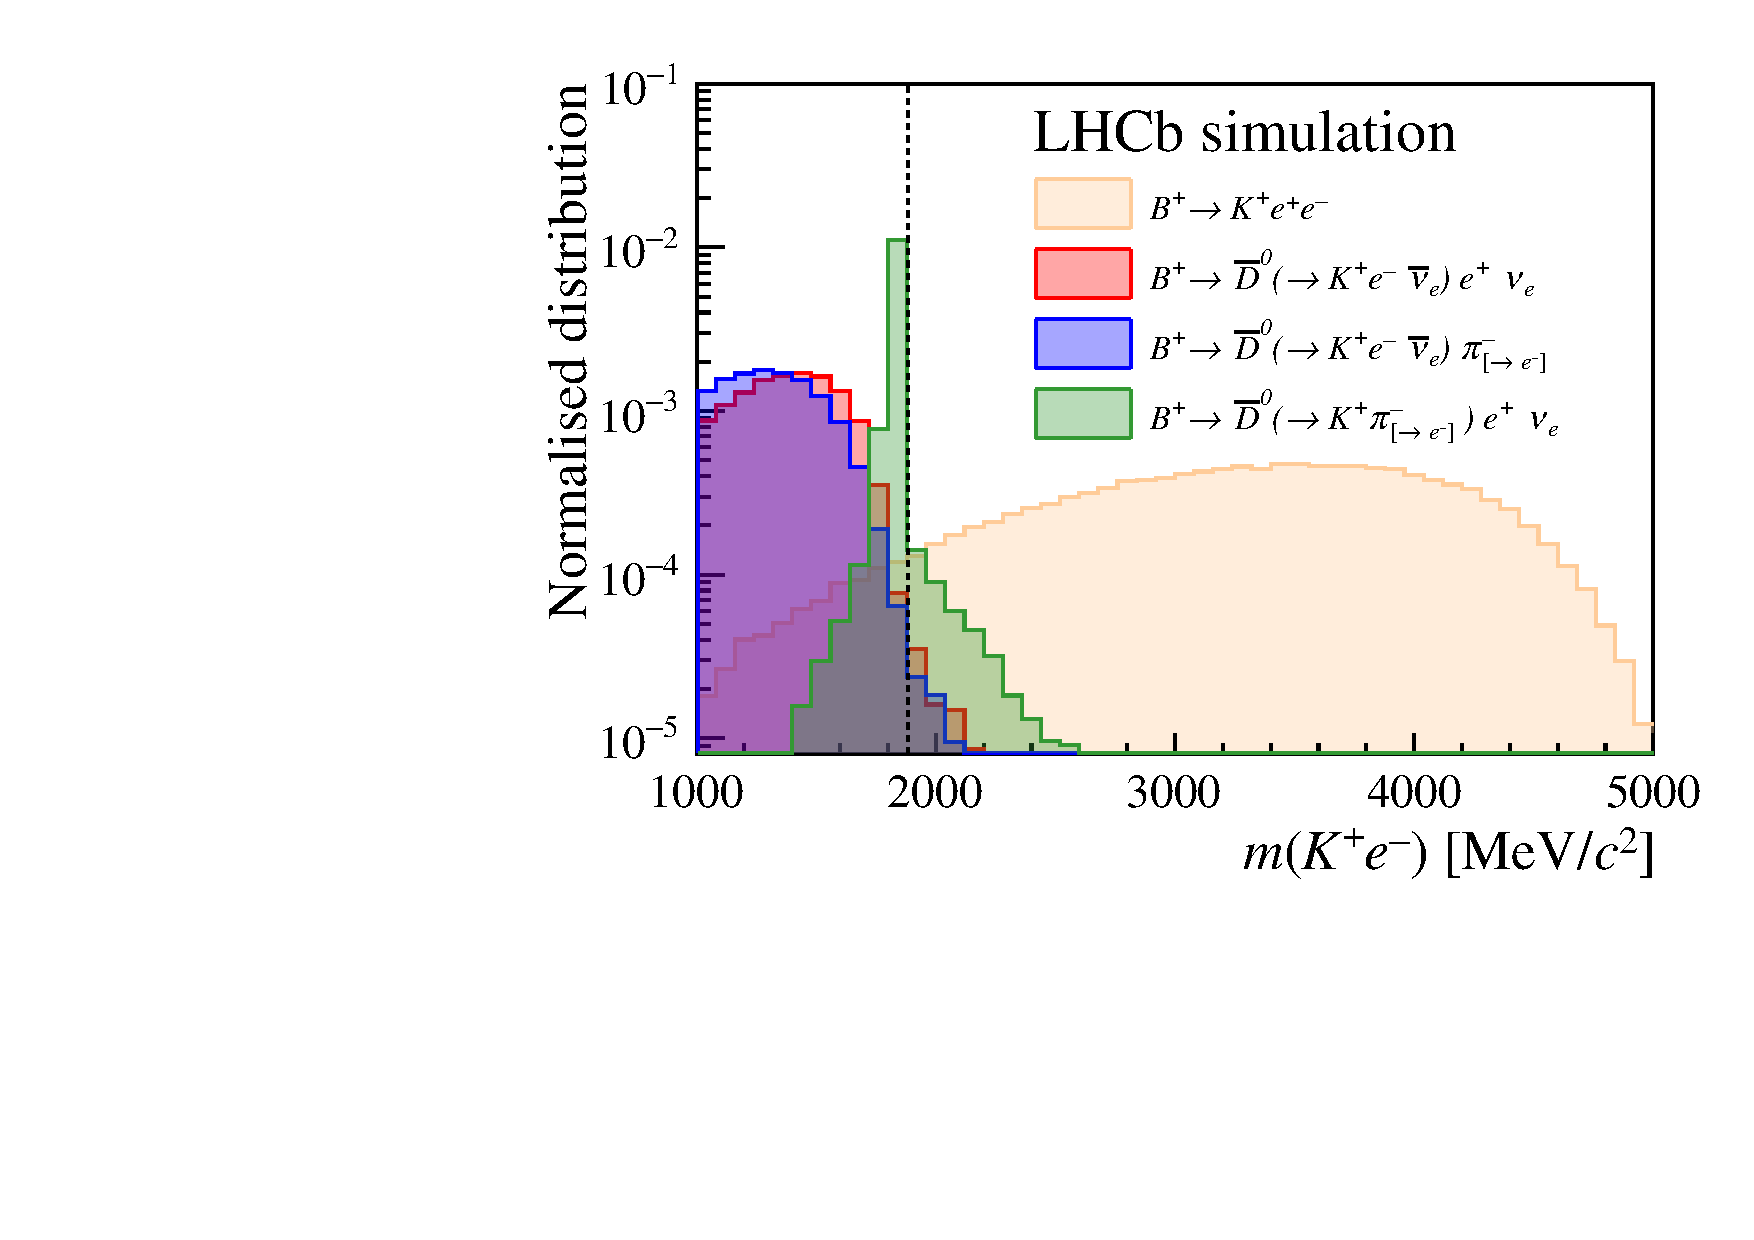
\includegraphics[width=0.48\linewidth]{figures/Fig5a.pdf}
      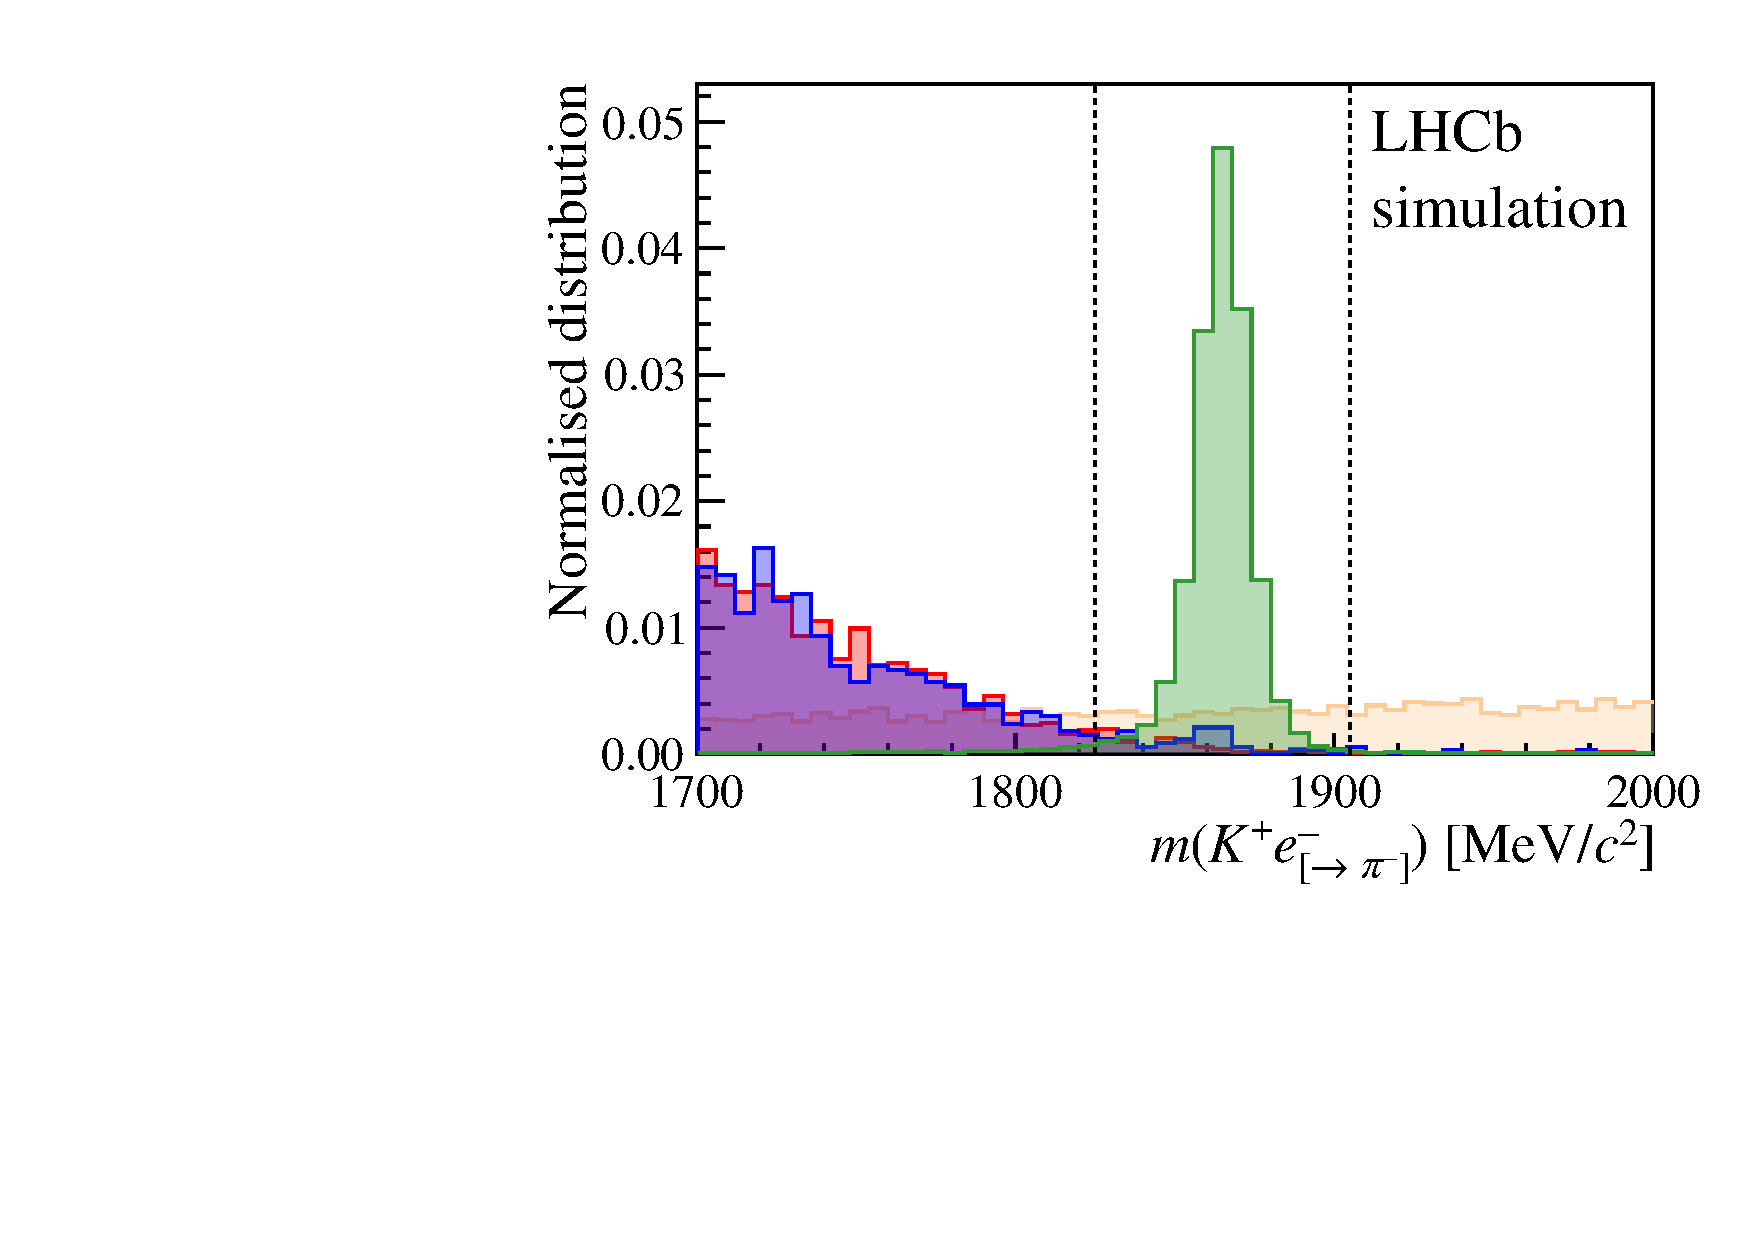
\includegraphics[width=0.48\linewidth]{figures/Fig5b.pdf}
   \end{center}
    \vspace*{-0.5cm}
   \caption{Simulated $K^+e^-$ mass distributions for  signal and various cascade background samples. The distributions are all normalised to unity.  (Left, with log $y$-scale)
   the bremsstrahlung correction to the momentum of the electron is applied, resulting in a tail to the right. The region to the left of the vertical dashed line is rejected. (Right, with linear $y$-scale) the mass is computed only from the track information. The notation $\pi^-_{[\rightarrow e^-]}$ ($e^-_{[\rightarrow \pi^-]}$) is used to denote an electron (pion) that is misidentified as a pion (electron). The region between the dashed vertical lines is rejected. }\label{fig:cascadeVeto}
\end{figure}

Background from other exclusive $B$-hadron decays requires at least two particles to be misidentified. These include the decays \BuKpipi, and misreconstructed \BuJpsiKll and \BuPsiKll decays. In the latter two decays the kaon is misidentified as a lepton and the lepton (of the same electric charge) as a kaon. Such background is reduced to a negligible level by particle-identification criteria. Background from decays with a photon converted into an \epem pair are also negligible due to the \qsq selection.


\subsubsection*{Multivariate selection}

A Boosted Decision Tree (BDT)  algorithm~\cite{Breiman} with gradient boosting~\cite{GradBoost} is used to reduce combinatorial background. For the nonresonant muon mode and for each of the three different trigger categories of the 
nonresonant electron mode, a single BDT classifier is trained for the 7 and $8\tev$ data, and an additional classifier is trained for the $13\tev$ data. The BDT output is not strongly correlated with \qsq and the same classifiers are used to select the respective resonant decays. 
In order to train the classifier, simulated nonresonant \BuKll decays are used as a proxy for the signal and nonresonant \Kll candidates selected from the data with $\mKll > 5.4\gevcc$ are used as a background sample. The $k$-folding technique is used in the training and testing~\cite{Blum:1999:BHB:307400.307439}. 
The classifier includes the following variables:  the  \pt of the \Bp, \Kp and dilepton candidates, and the minimum and maximum \pt of the leptons;  the \Bp, dilepton and \Kp \chisqip with respect to the associated PV, where \chisqip is defined as the difference in the vertex-fit \chisq of the PV reconstructed with and without the considered particle; the minimum and maximum \chisqip of the leptons; the \Bp vertex-fit quality; the statistical significance of the \Bp flight distance; and the angle between the \Bp candidate momentum vector and the direction between the associated PV and the \Bp decay vertex. 
For each of the classifiers, a requirement is placed on the output variable in order to maximise the predicted significance of the nonresonant signal yield. For the electron modes that dictate the \RK precision, this requirement reduces the combinatorial background by approximately $99\%$, while retaining $85\%$ of the signal mode. The muon BDT classifier has similar performance. In both cases the efficiency of the BDT selection has negligible dependence on \mKll in the regions used to determine the event yields. 

\subsubsection*{Calibration of simulation} 

The simulated data used in this analysis are produced using the software described in Refs.~\cite{Sjostrand:2006za,*Sjostrand:2007gs,LHCb-PROC-2010-056,Lange:2001uf,Allison:2006ve, *Agostinelli:2002hh,LHCb-PROC-2011-006}. Bremsstrahlung emission in the decay of particles is simulated using the \photosplusplus software in the default configuration~\cite{ Davidson:2010ew}, which is observed to agree with a full quantum electrodynamics calculation at the level of $1\%$~\cite{Bordone:2016gaq}.

Simulated events are weighted to correct for the imperfect modelling using control channels. The \Bu production kinematics are corrected using \BuJpsiKll events. The particle-identification performance is calibrated using data, where the species of particles in the final state can be unambiguously determined purely on the basis of the kinematics. 
The calibration samples consist of $\decay{\Dstarp}{\Dz(\to\Km\pip)\pip}$, $\decay{\jpsi}{\mumu}$, and \BuJpsiKee decays, from which kaons, muons, and electrons, respectively, can be selected without applying particle-identification requirements. The performance of the particle-identification requirements is then evaluated from the proportion of events in these samples which fulfil the particle-identification selection criteria. The trigger response is corrected using weights applied to simulation as a function of variables relevant to the trigger algorithms. The weights are calculated by requiring that simulated \BuJpsiKll events  exhibit the same trigger performance as the control data. The \BuJpsiKll events selected from the data have also been used to demonstrate control of the electron track-reconstruction efficiency at the percent level~\cite{Aaij:2019vvl}.
Whenever \BuJpsiKll events are used to correct the simulation, the correlations between calibration and measurement samples are taken into account in the results and cross-checks presented in the article. 

\subsubsection*{Likelihood fit} 

An unbinned extended maximum-likelihood fit is made to the \mKee and \mKmm distributions of nonresonant candidates. The value of \RK is a fit parameter, which is related to the signal yields and efficiencies according to,  
\begin{eqnarray}
    \label{eq:RKdetail}
       \RK &=&\frac{N(\BuKmm)}{\varepsilon(\BuKmm)}\cdot\frac{\varepsilon(\BuKee)}{N(\BuKee)} \times \nonumber\\
 & & \frac{\varepsilon(\BuJpsiKmm)}{N(\BuJpsiKmm)}\cdot\frac{N(\BuJpsiKee)}{\varepsilon(\BuJpsiKee)} \,, 
\end{eqnarray}
\noindent where $N(X)$  indicates the  yield  of  decay  mode $X$,  which  is  obtained from a fit to the invariant mass \mKll (or \mKllconst) with a suitable requirement on \qsq, and $\varepsilon(X)$ is the efficiency for selecting decay mode $X$. In order to take into account the correlation between the selection efficiencies, the \mKee and \mKmm distributions of nonresonant candidates in each of the different trigger categories and data-taking periods are fitted simultaneously. 

The mass-shape parameters are derived from the calibrated simulation. The four signal modes are modelled by multiple Gaussian functions with  power-law tails on both sides of the peak~\cite{Skwarnicki:1986xj,Santos:2013gra} although the differing detector response gives different shapes for the electron and muon modes. The signal mass shapes of the electron modes are described with the sum of three distributions, which model whether the ECAL energy deposit from a bremsstrahlung photon was added to both, either, or neither of the \epm candidates. The expected values from simulated events are used to constrain the fraction of signal decays in each of these categories.

Data are used to correct the simulated $K\pi$ mass spectrum for \BuBdKpiplusee and \BuBdKpijpsi decays~\cite{LHCb-PAPER-2016-025}. The calibrated simulation is used subsequently to obtain the \mKll mass shape and relative fractions of these background components. In order to accommodate possible lepton-universality violation in these partially reconstructed processes, which are underpinned by the same $\bquarkbar\to\squarkbar$ quark-level transitions as those of interest, the overall yield of such decays is left to vary freely in the fit. The shape of the \BuJpsipi background contribution is taken from simulation but the size with respect to the \BuJpsiK mode is constrained using the known ratio of the relevant branching fractions~\cite{LHCb-PAPER-2016-051, PDG2020} and efficiencies.

In the fits to nonresonant \BuKee candidates, the mass shape of the background from \BuJpsiKee decays with an emitted photon that is not reconstructed is also taken from simulation and, adjusting for the relevant selection efficiency, its yield is constrained to the value from the fit to the resonant mode within its uncertainty.   
In all fits, the combinatorial background is modelled with an exponential function with a freely varying yield and shape.

The fits to the nonresonant (resonant) decay modes in different data-taking periods and trigger categories are shown in Fig.~\ref{fig:nonresfits_categories}  (Fig.~\ref{fig:resfits_categories}).
For the resonant modes the results from independent fits to each period/category are shown. Conversely, the nonresonant distributions show the projections from the simultaneous fit across data taking periods and trigger categories that is used to obtain \RK. The fitted yields for the resonant and nonresonant decays are given in Table~\ref{tab:yields}. 

\begin{table}[b]
\centering
\caption{Yields of the  nonresonant and resonant decay modes obtained from the fits to the data.} \label{tab:yields}
\begin{tabular}{lc}
\toprule
Decay mode  &   Yield             \\
\midrule
\BuKee      &   $\phantom{0\,00}1\,640 \pm \phantom{0\,0}70$ \\
\BuKmm      &   $\phantom{0\,00}3\,850 \pm \phantom{0\,0}70$ \\
\BuJpsiKee  &   $\phantom{0\,}743\,300 \pm \phantom{0\,}900$ \\
\BuJpsiKmm  &   $2\,288\,500 \pm 1\,500$      \\
\bottomrule
\end{tabular}
\end{table}


\begin{figure}
    \centering
    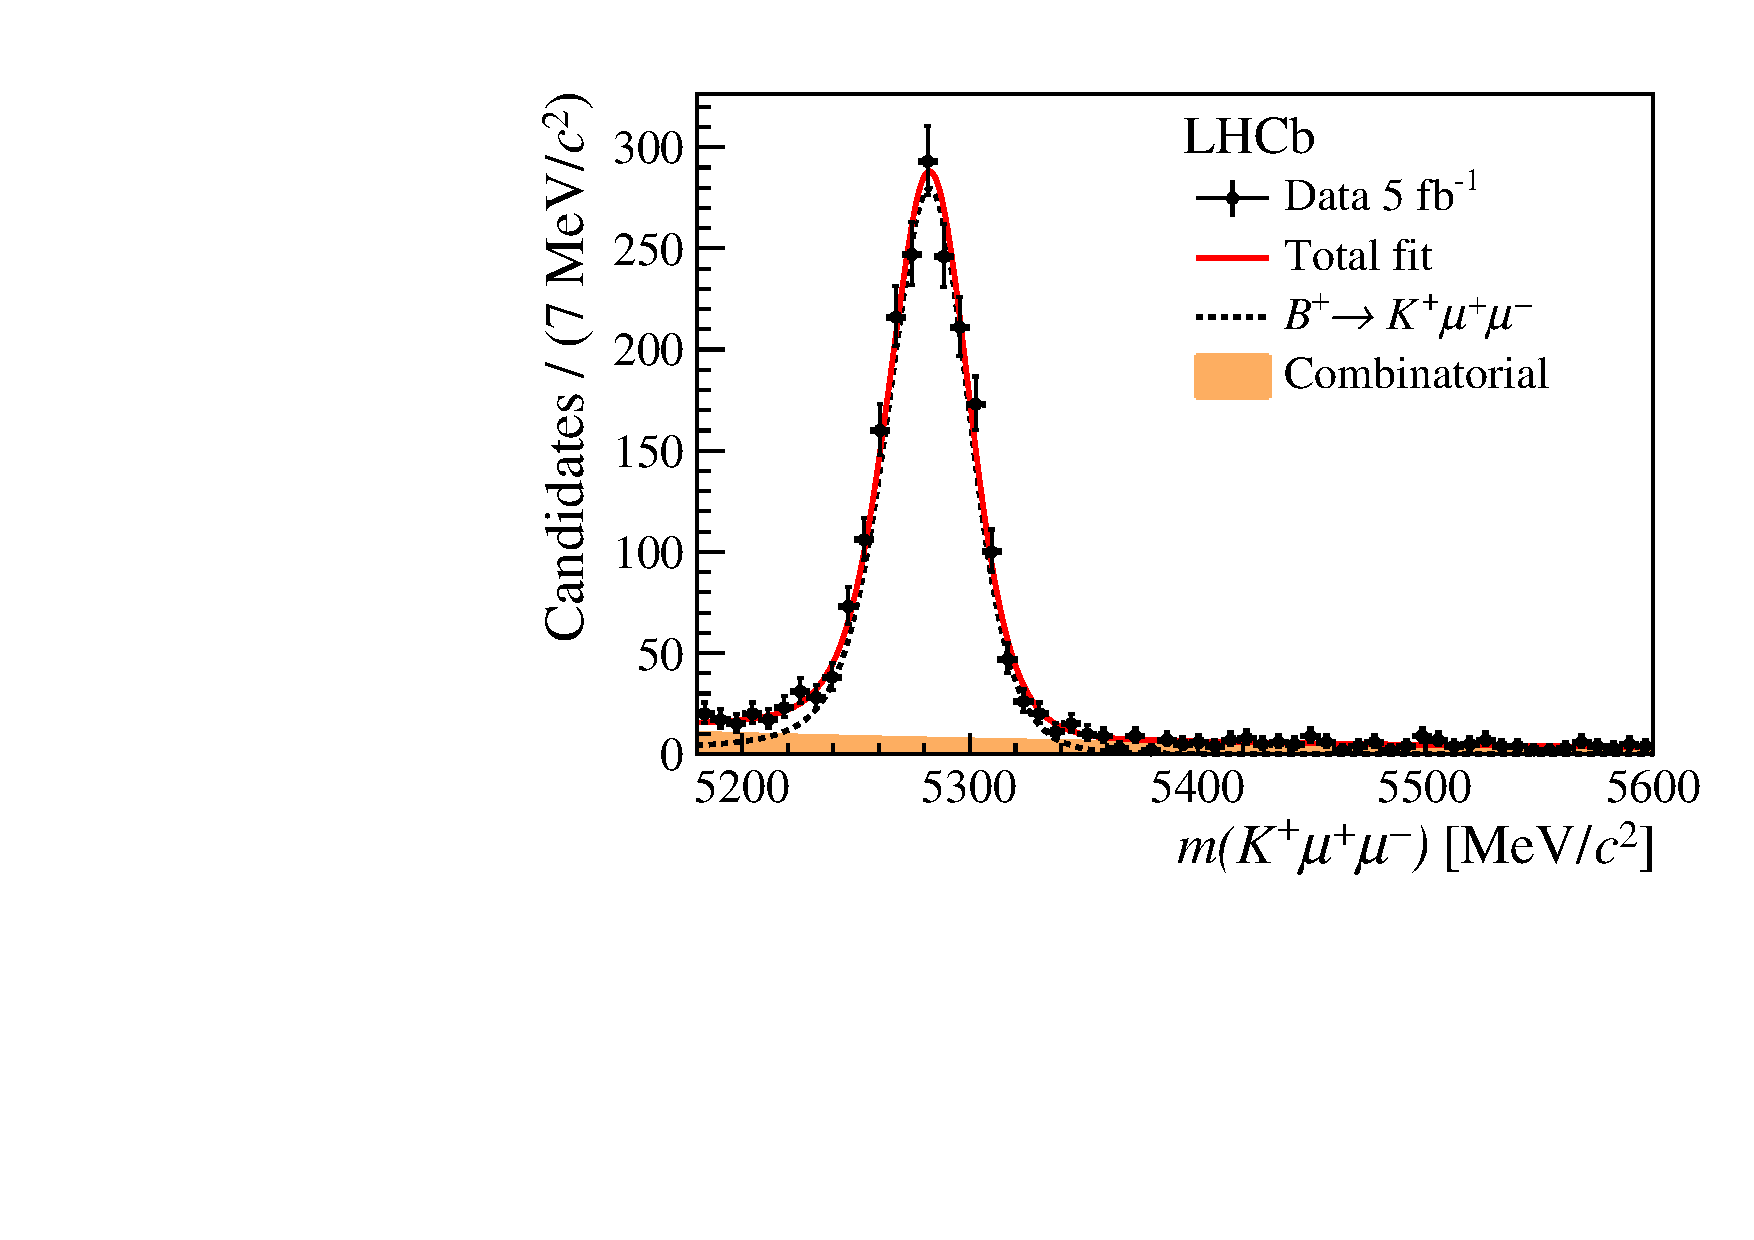
\includegraphics[width=0.45\textwidth]{figures/Fig6a.pdf}
    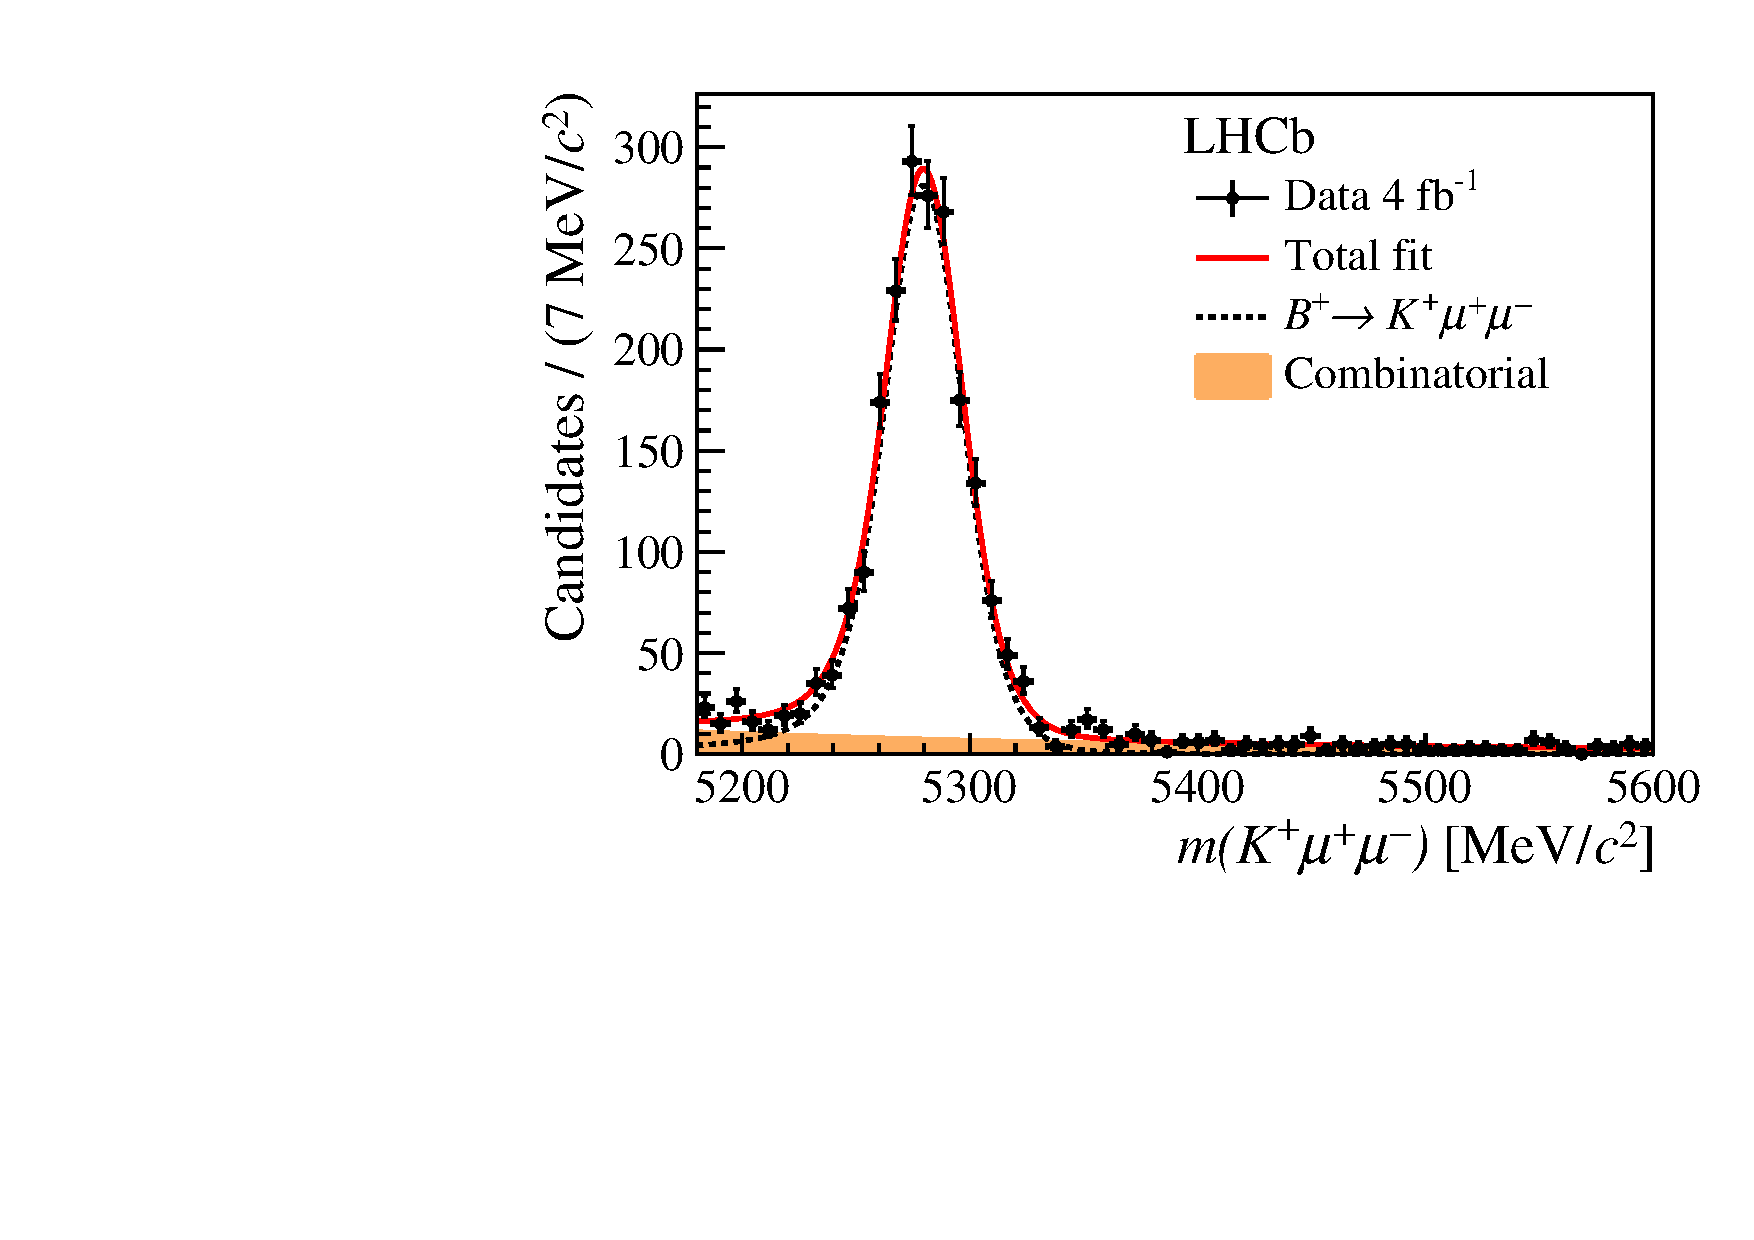
\includegraphics[width=0.45\textwidth]{figures/Fig6b.pdf}

    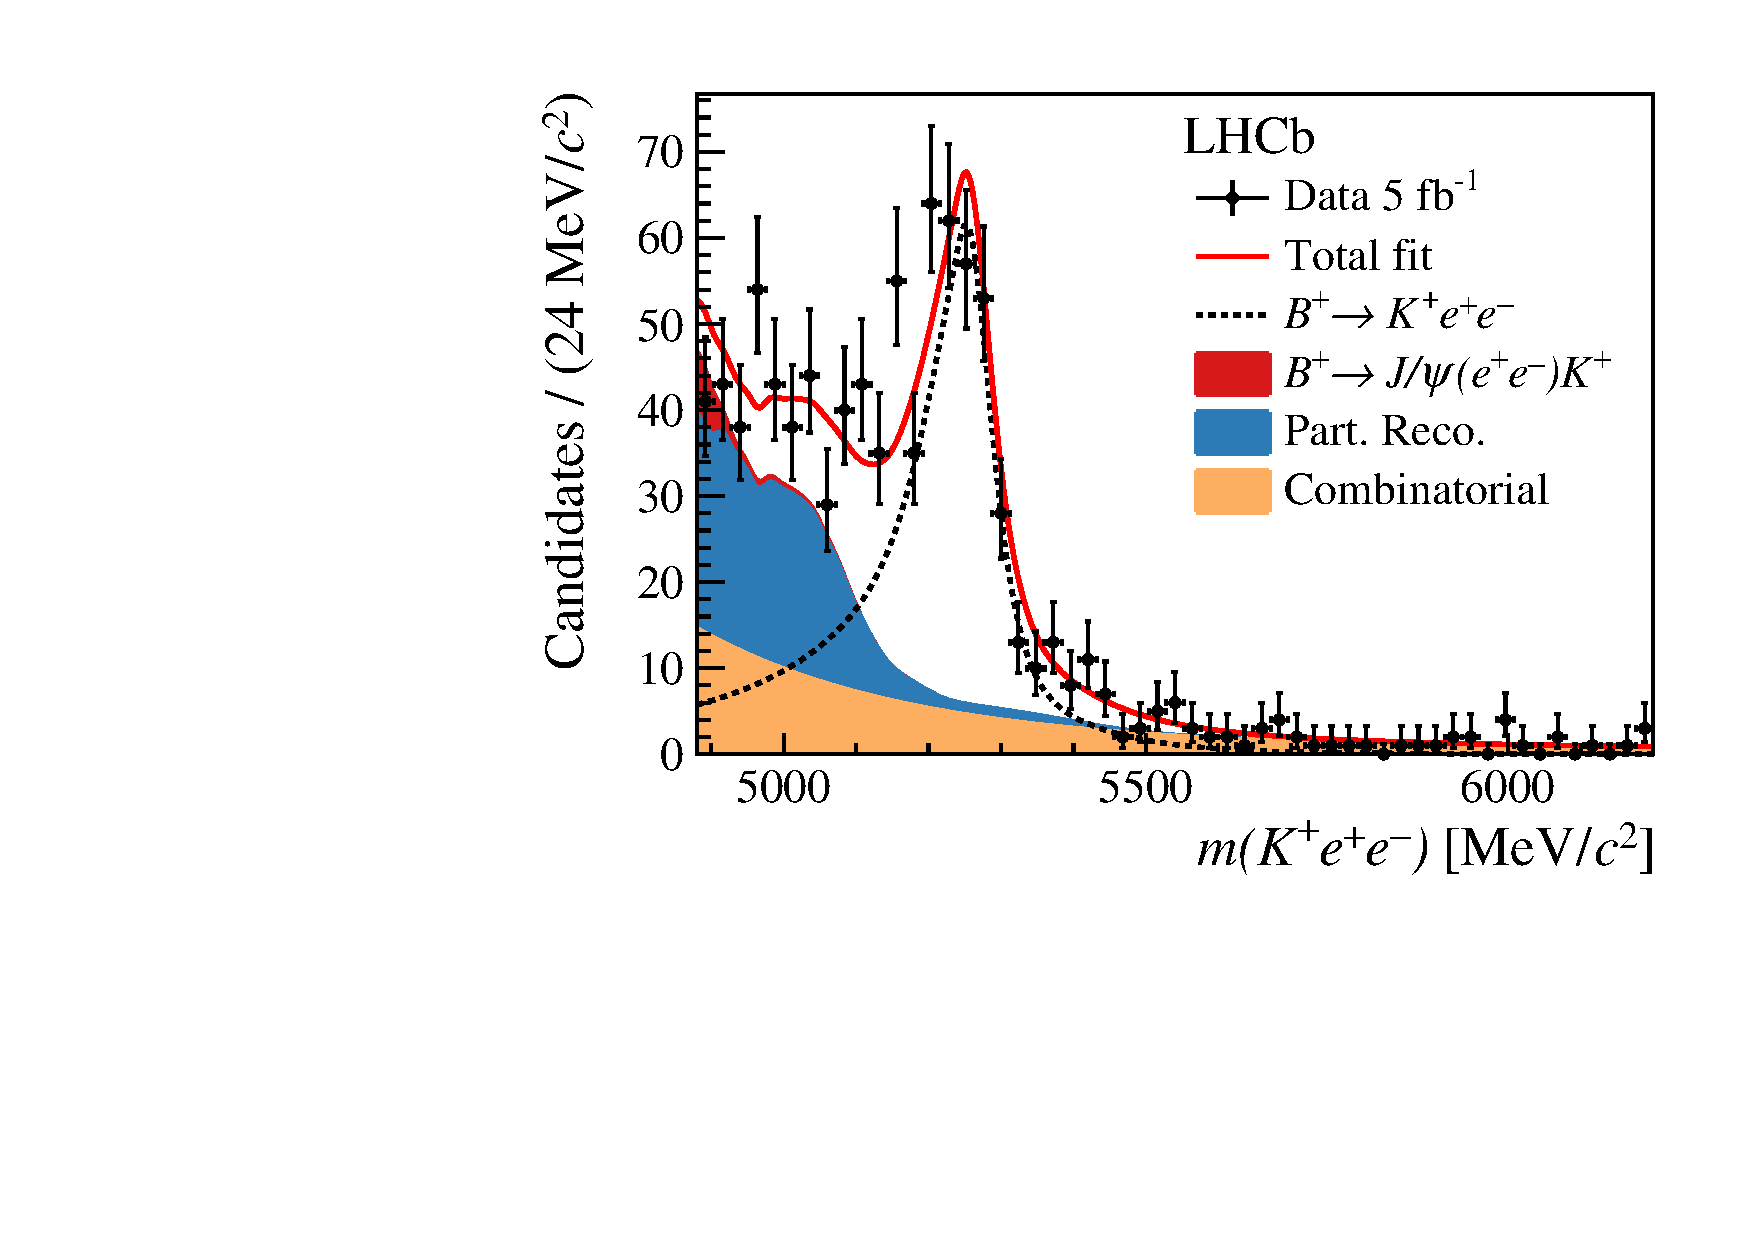
\includegraphics[width=0.45\textwidth]{figures/Fig6c.pdf}
    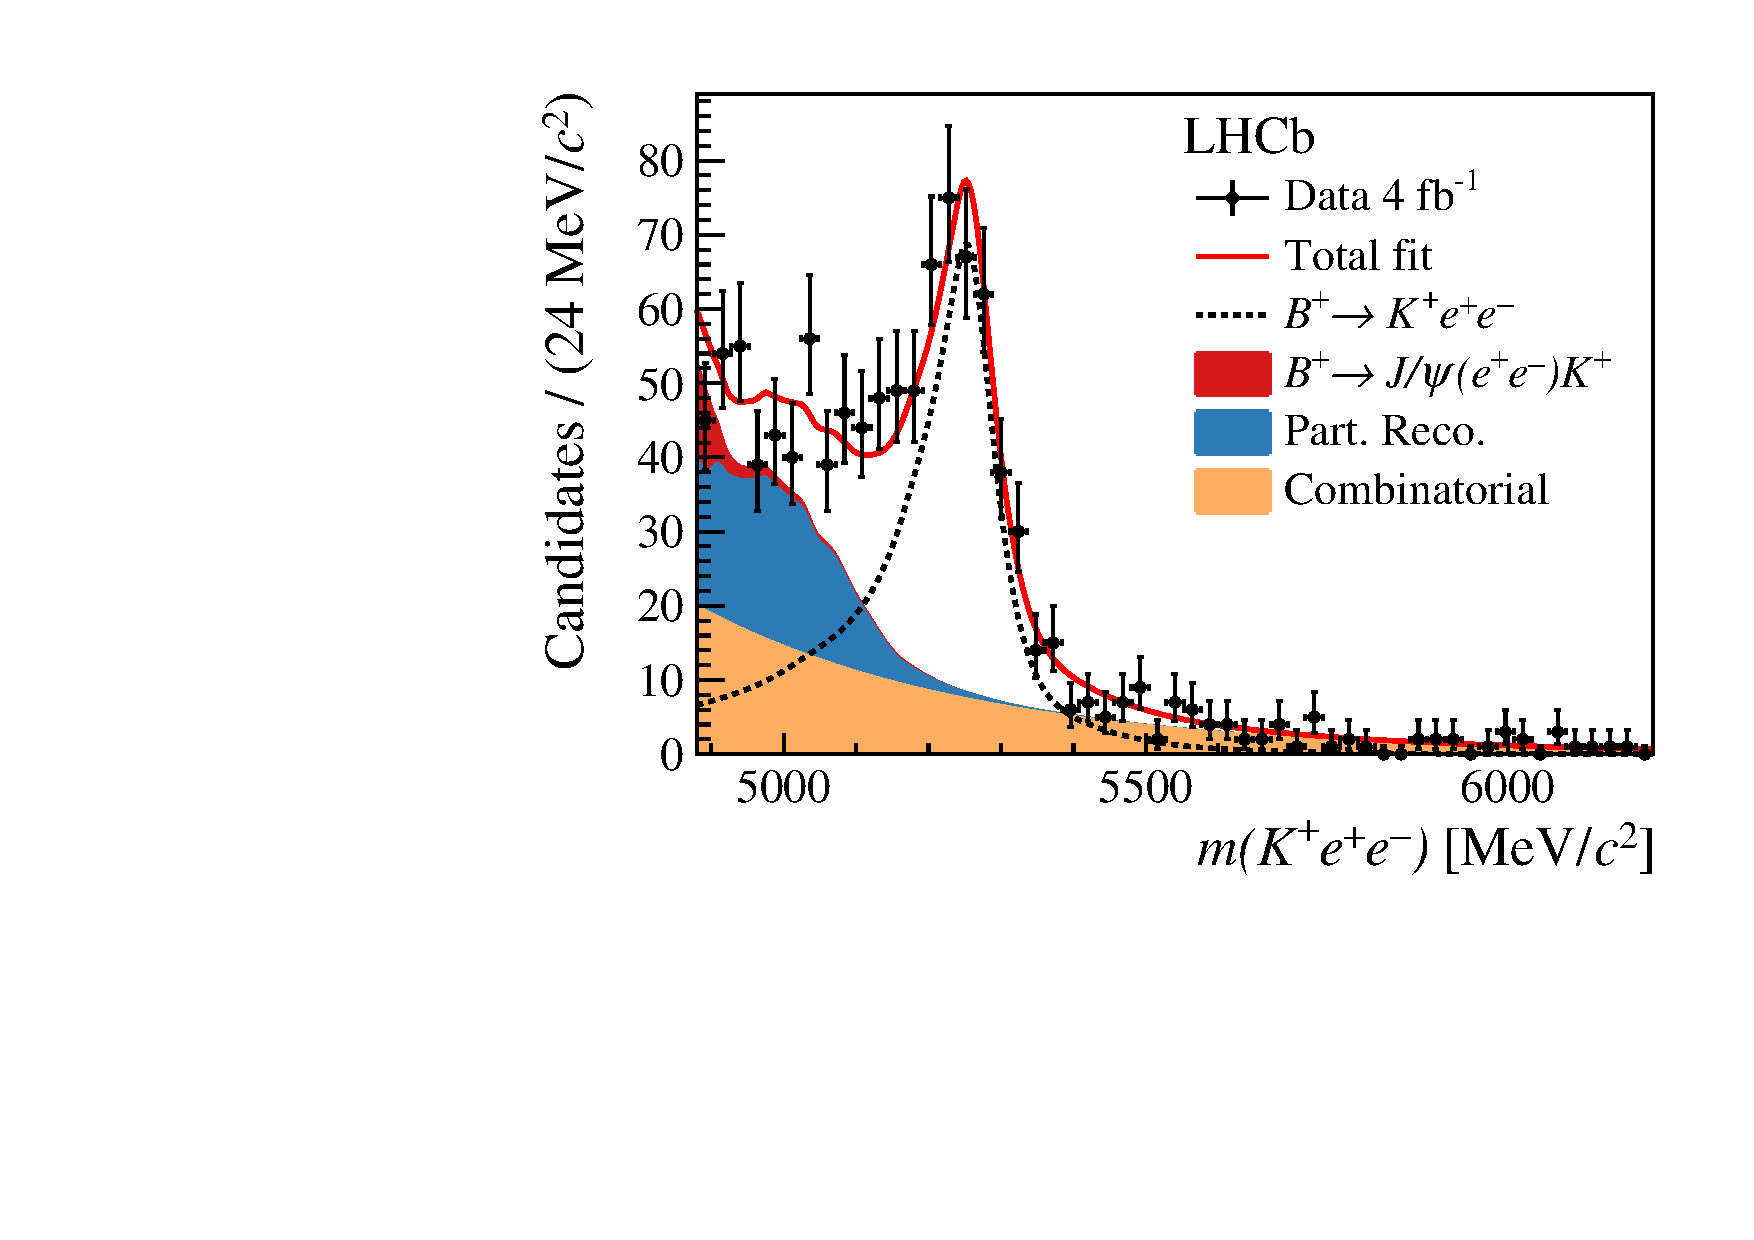
\includegraphics[width=0.45\textwidth]{figures/Fig6d.pdf}
    
    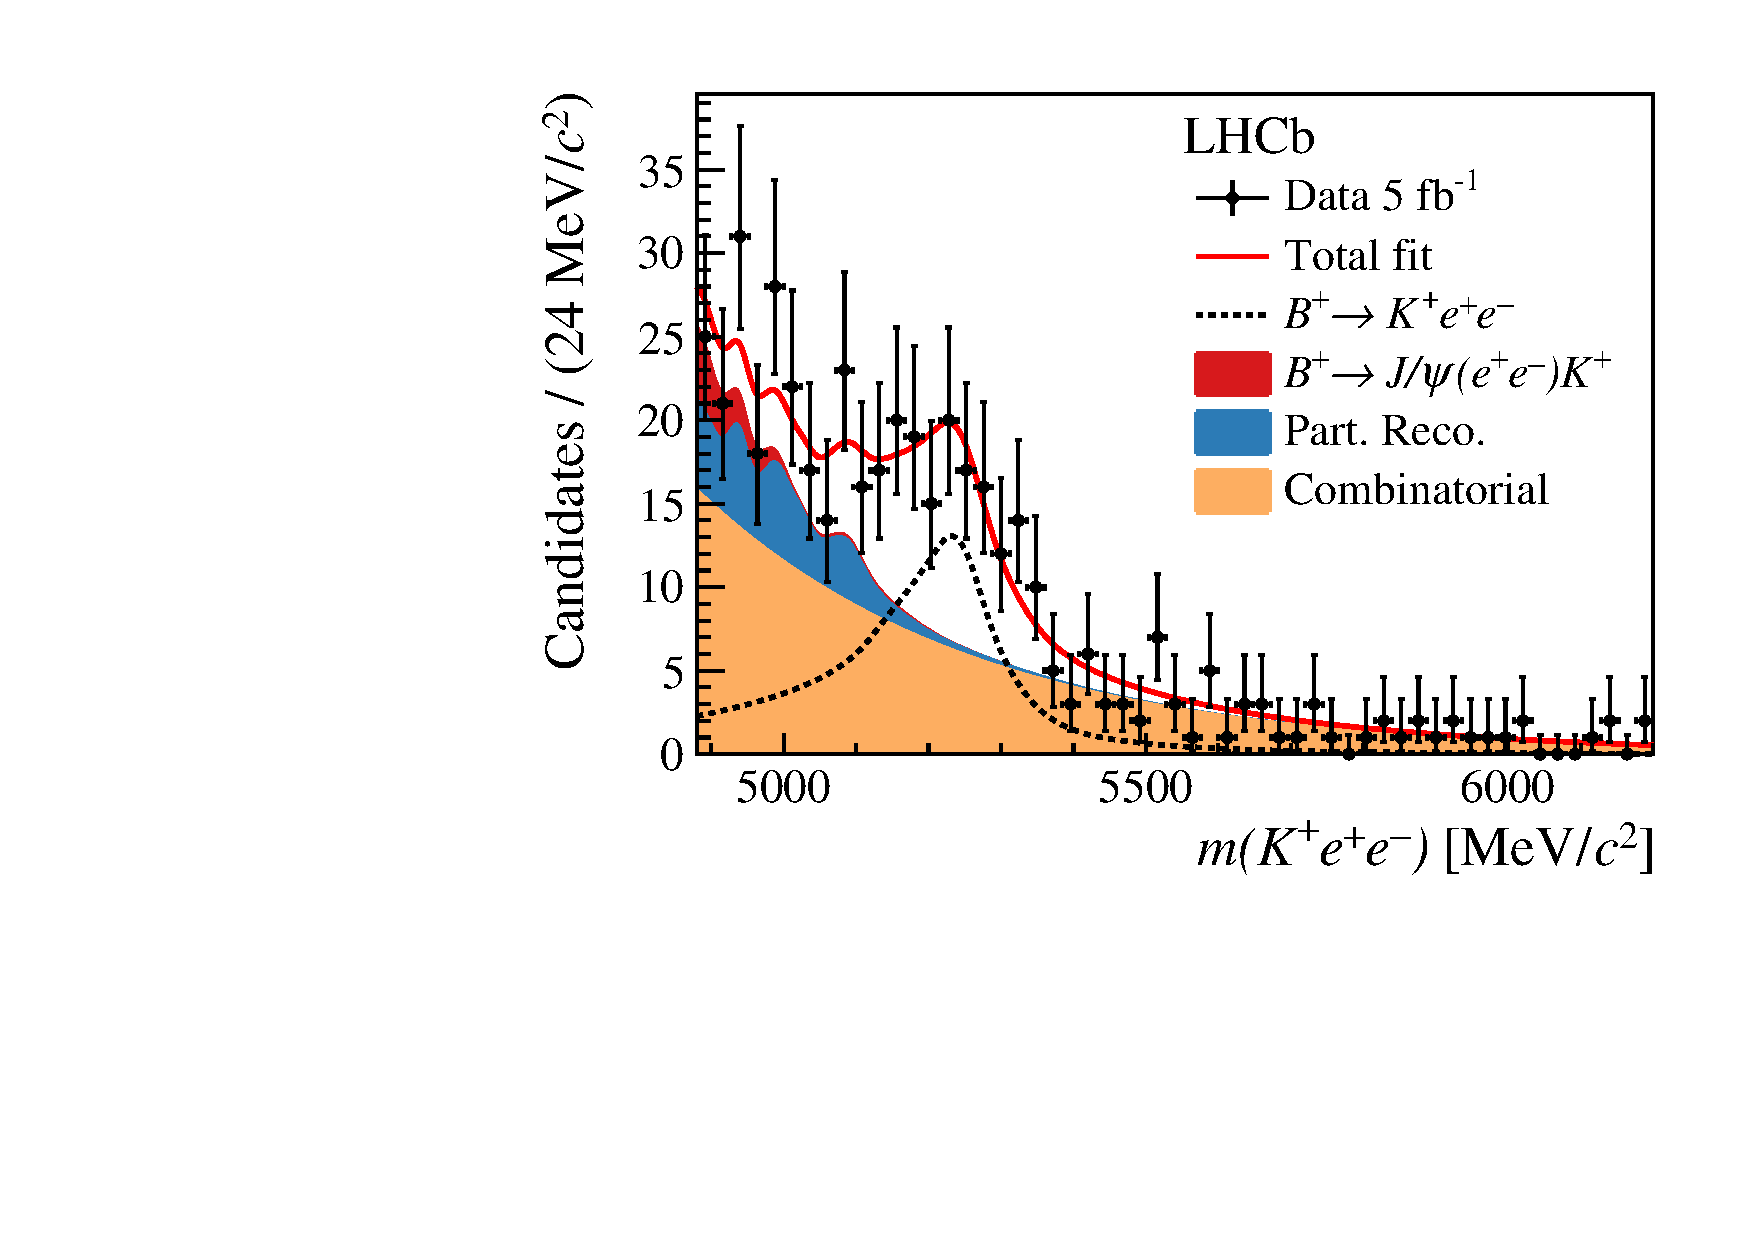
\includegraphics[width=0.45\textwidth]{figures/Fig6e.pdf}
    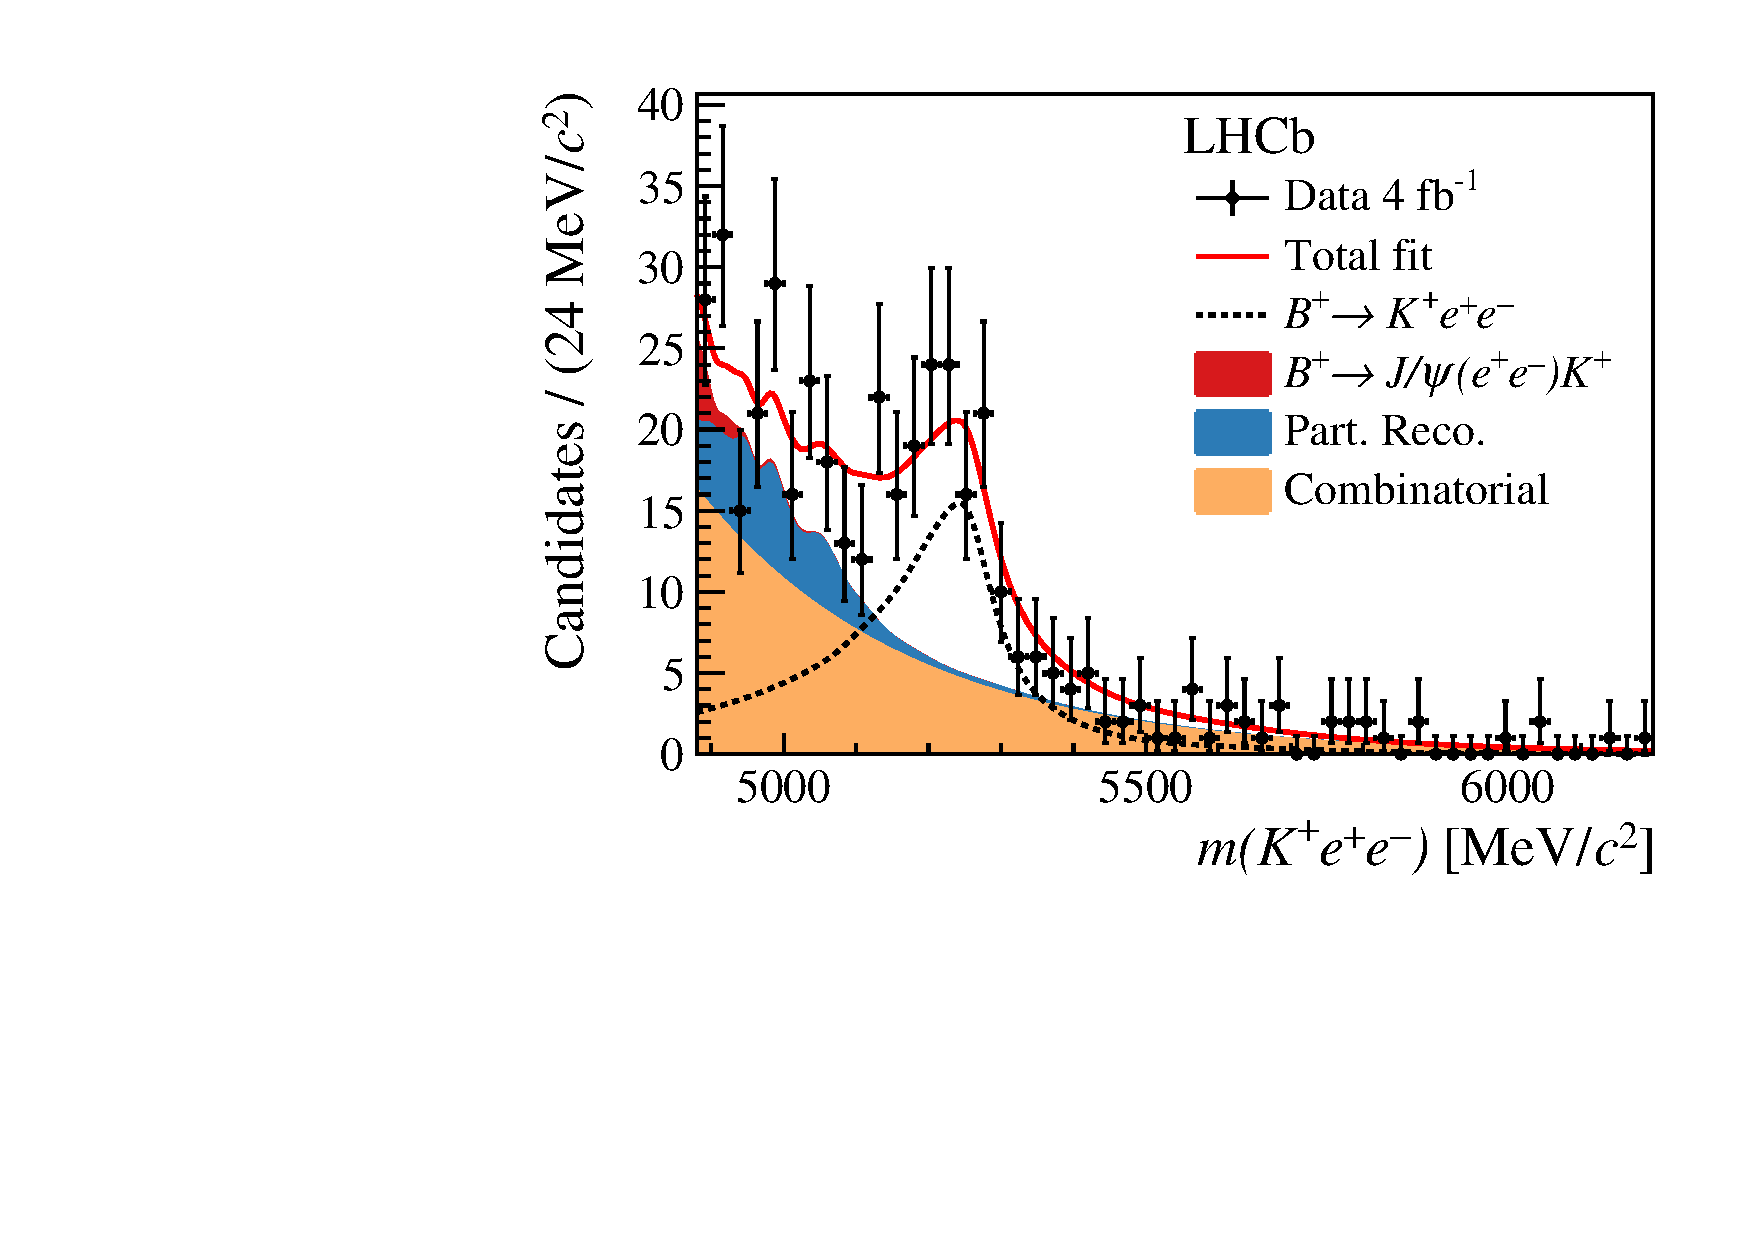
\includegraphics[width=0.45\textwidth]{figures/Fig6f.pdf}
    
    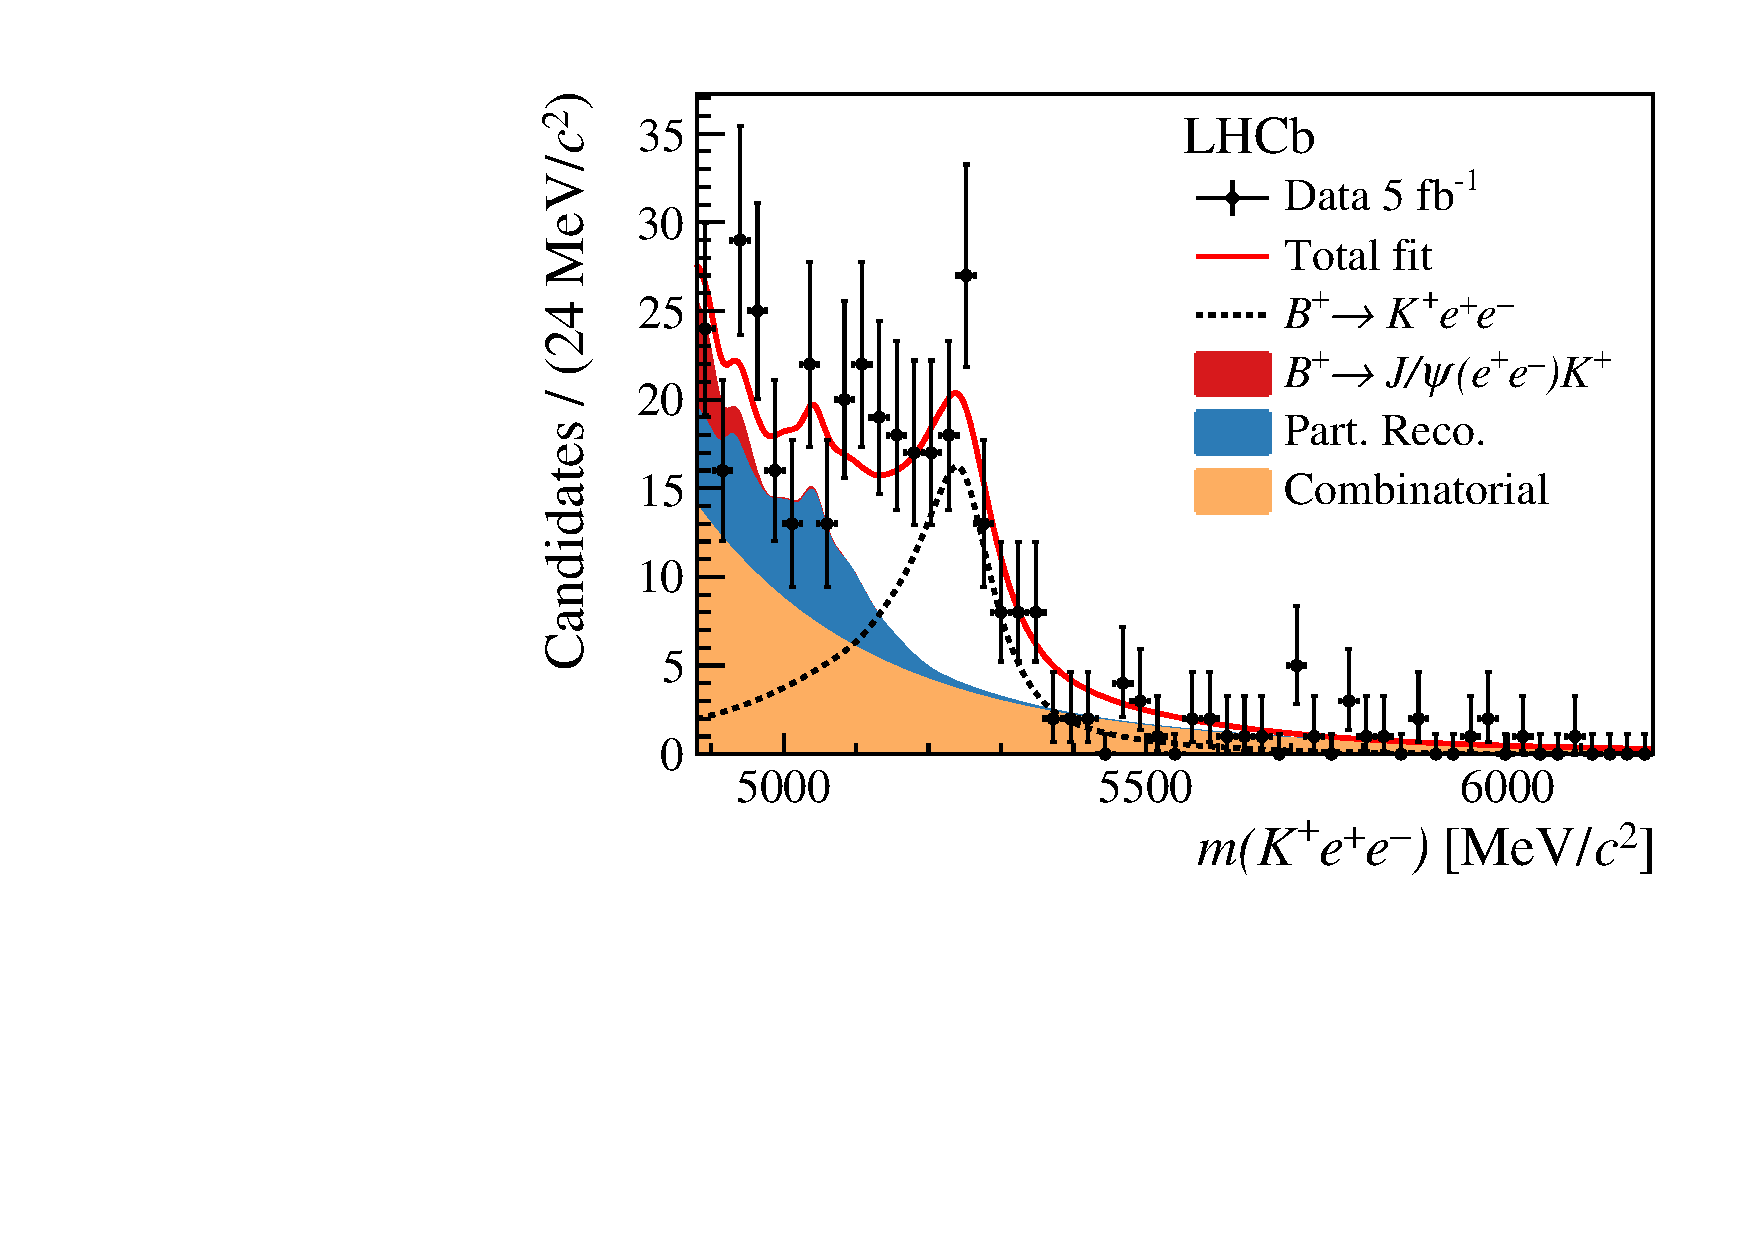
\includegraphics[width=0.45\textwidth]{figures/Fig6g.pdf}
    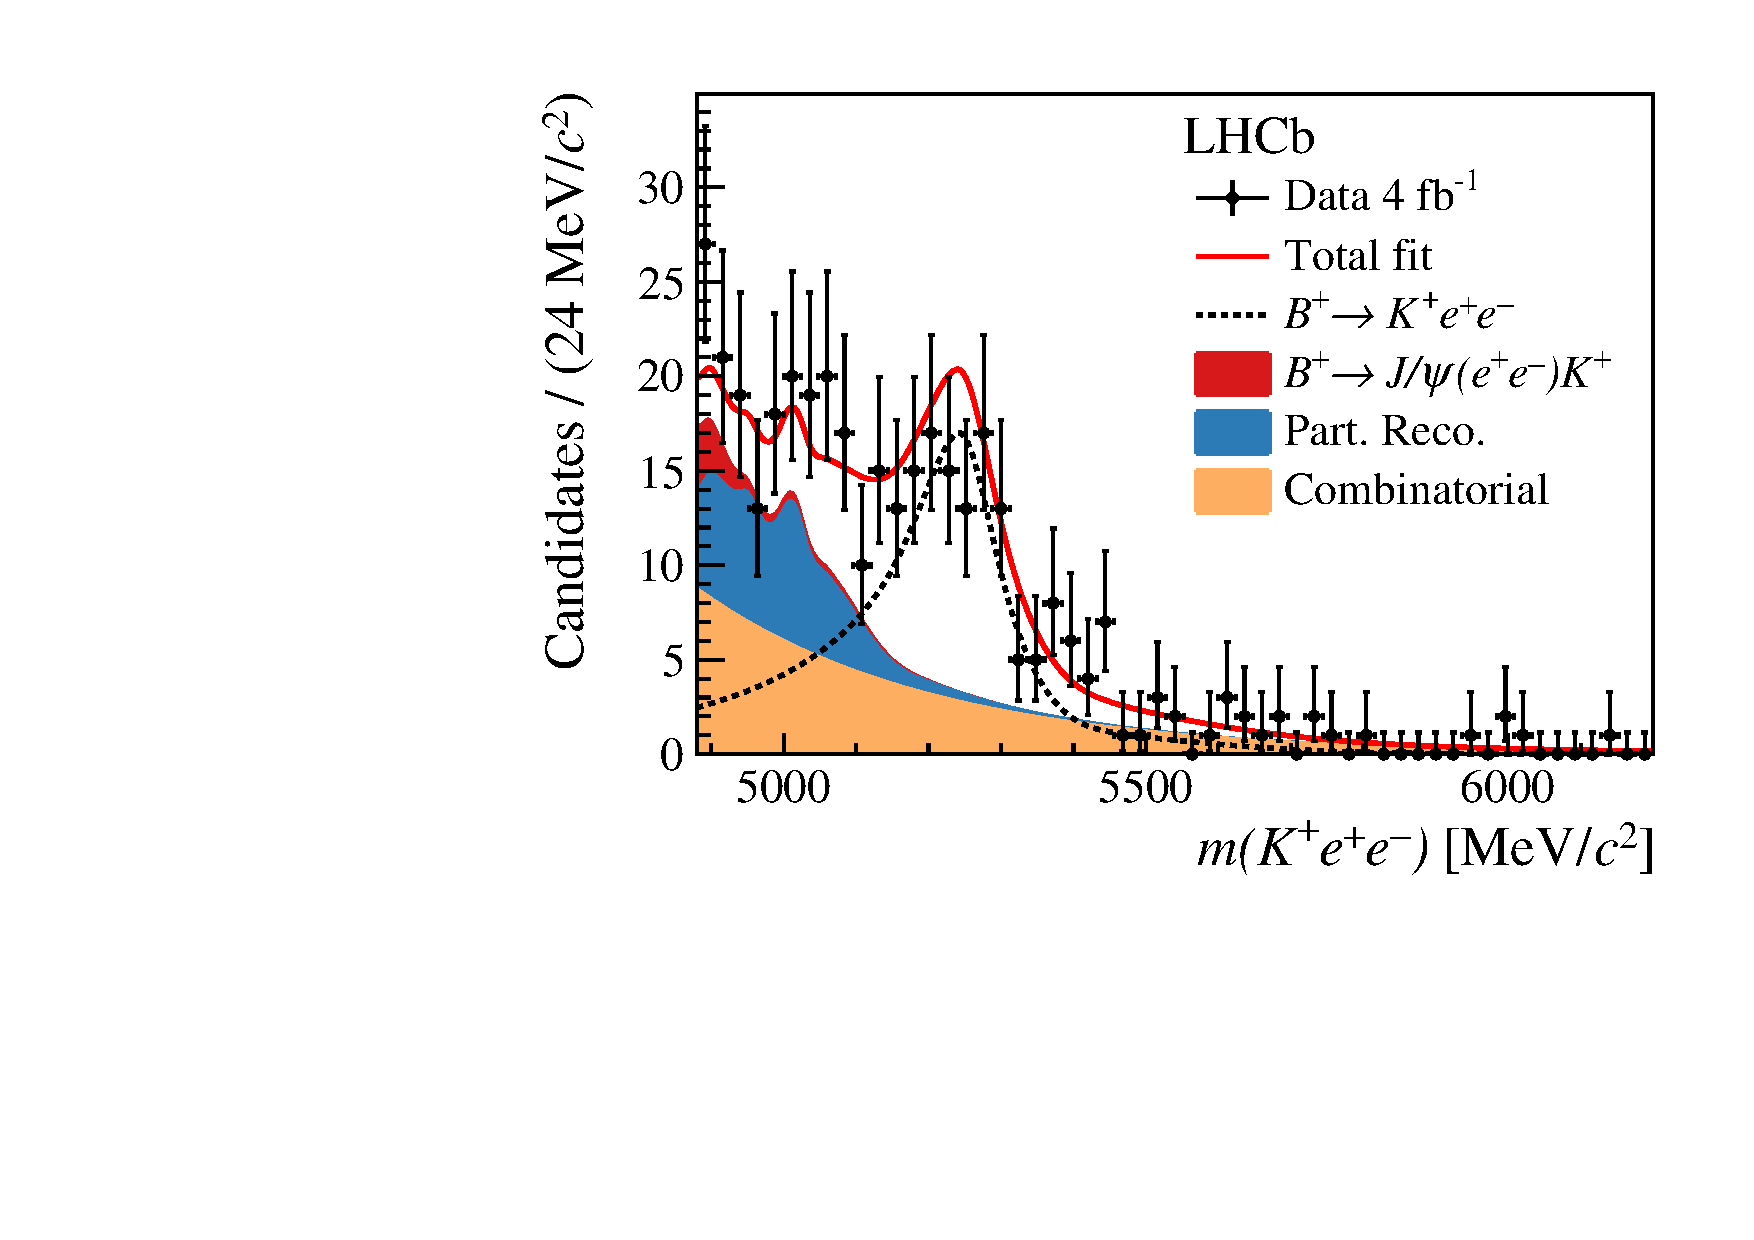
\includegraphics[width=0.45\textwidth]{figures/Fig6h.pdf}
    \caption{Candidate invariant mass distributions. Distribution of the invariant mass \mKll for nonresonant candidates in the (left) sample previously analysed~\cite{LHCb-PAPER-2019-009} and (right) the new data sample. The top row shows the fit to the muon modes and the subsequent rows the fits to the electron modes triggered by (second row) one of the electrons, (third row) the kaon and (last row) by other particles in the event. The fit projections are superimposed.
    }
    \label{fig:nonresfits_categories}
\end{figure}


\begin{figure}
    \centering
    % \includegraphics[width=0.45\textwidth]{figures/FigS5a.pdf}
    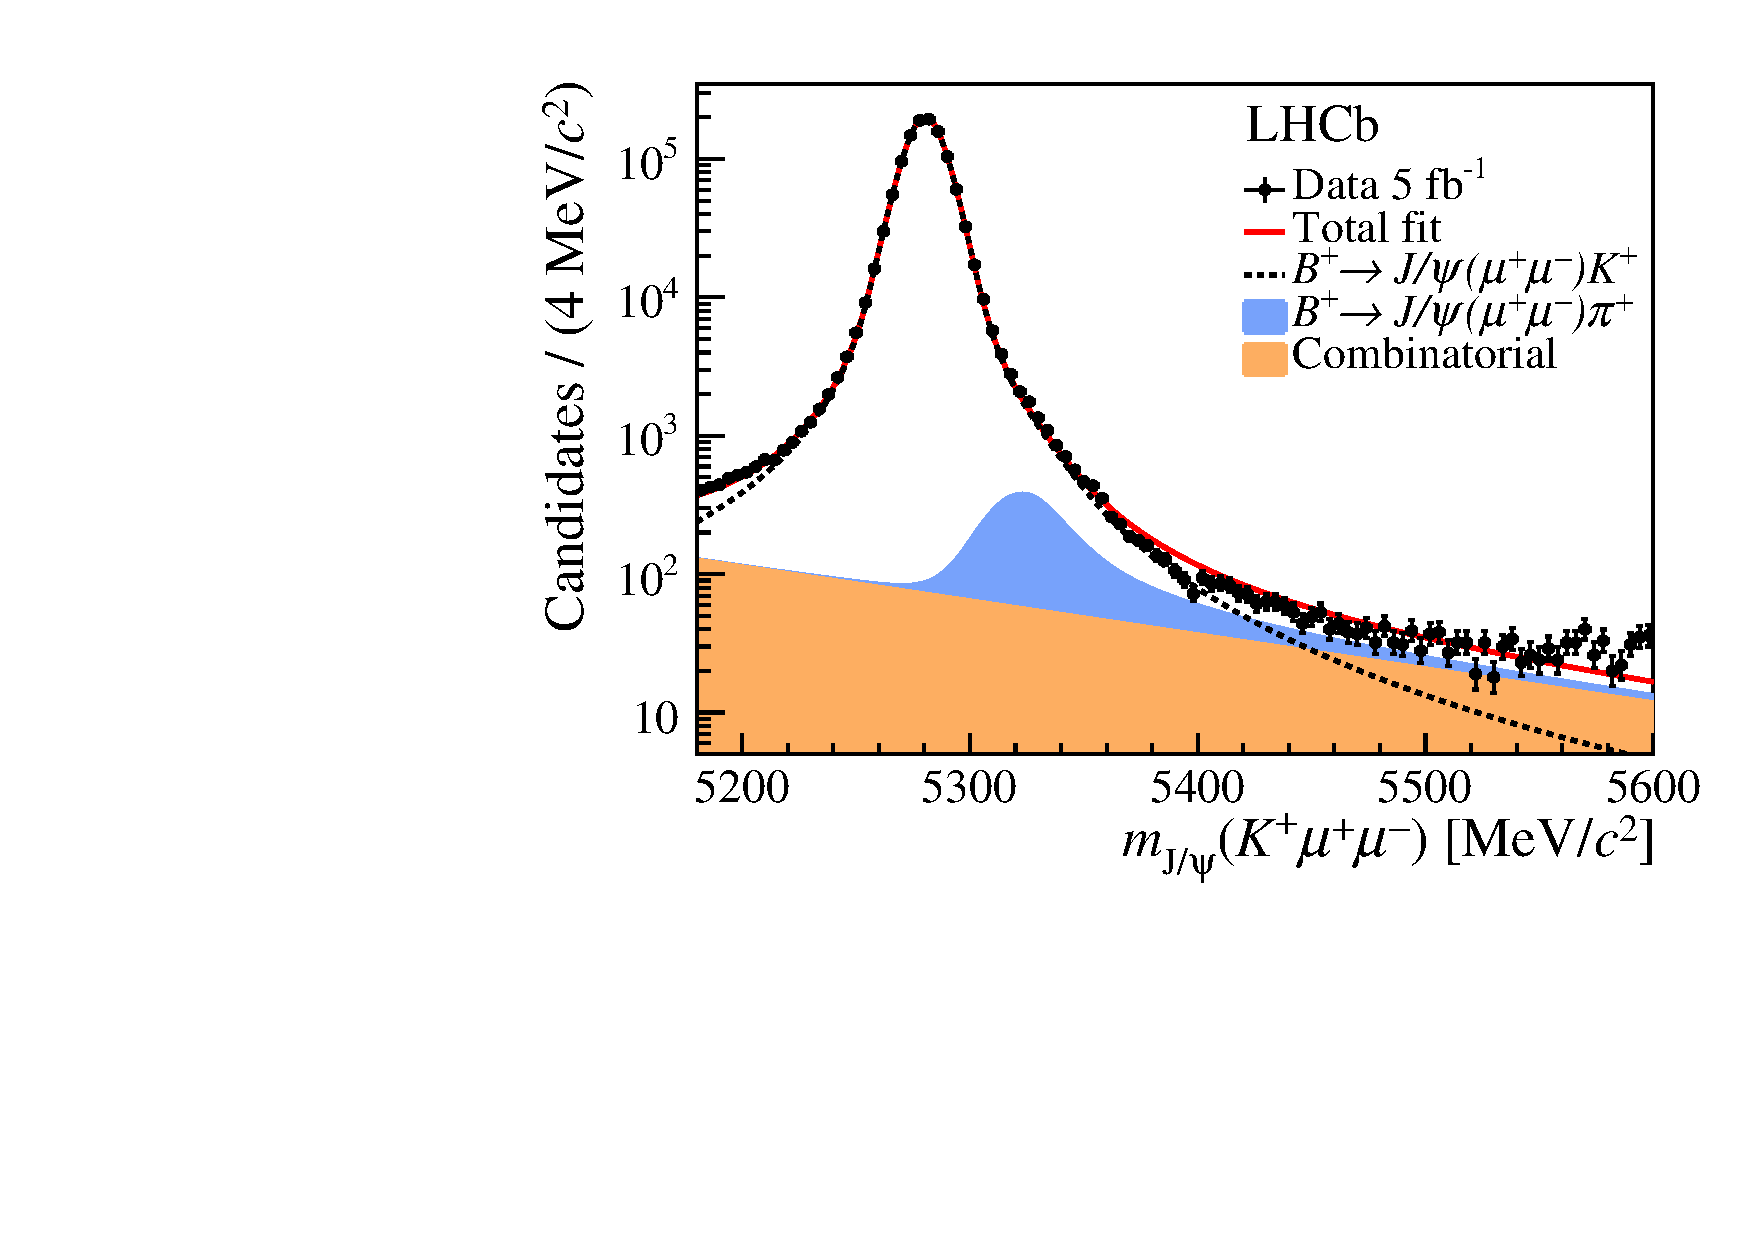
\includegraphics[width=0.45\textwidth]{figures/Fig7a.pdf}
    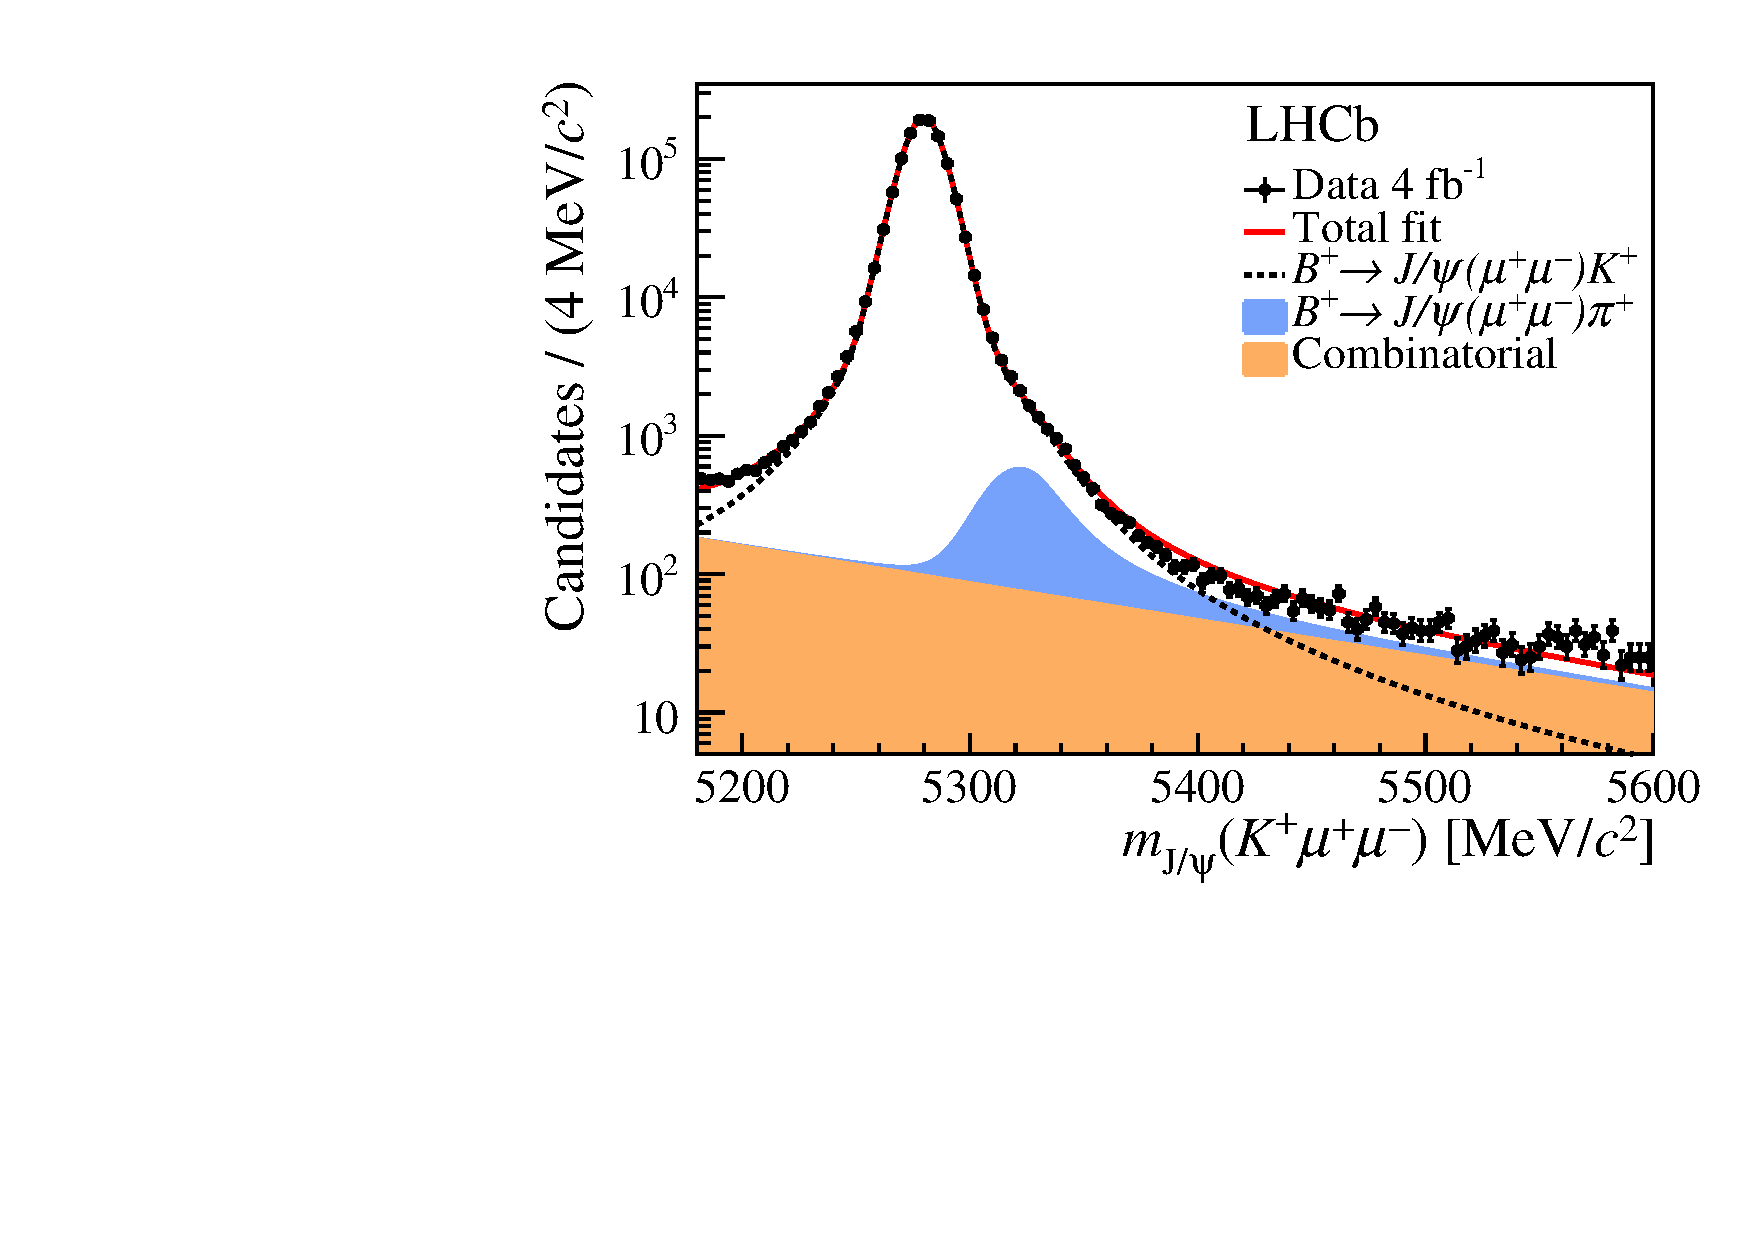
\includegraphics[width=0.45\textwidth]{figures/Fig7b.pdf}
    
    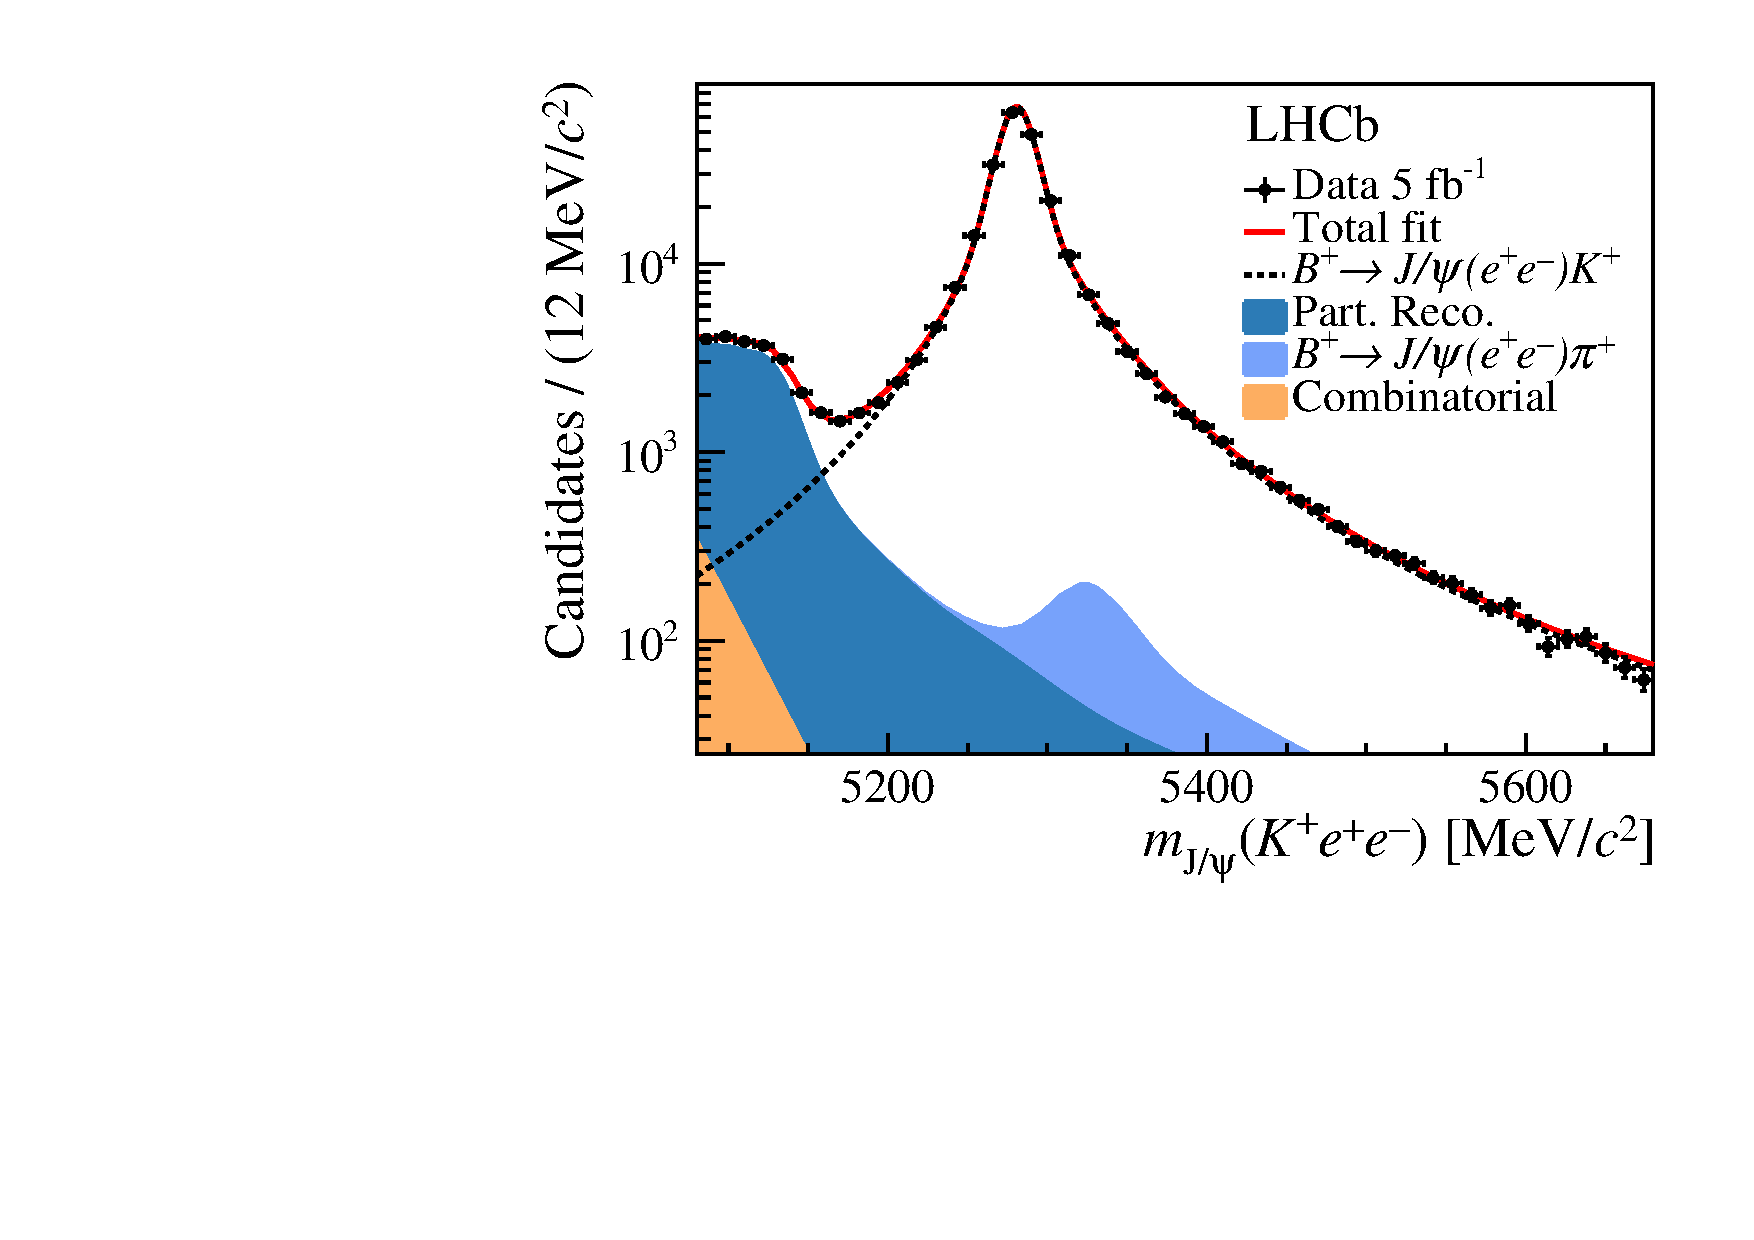
\includegraphics[width=0.45\textwidth]{figures/Fig7c.pdf}
    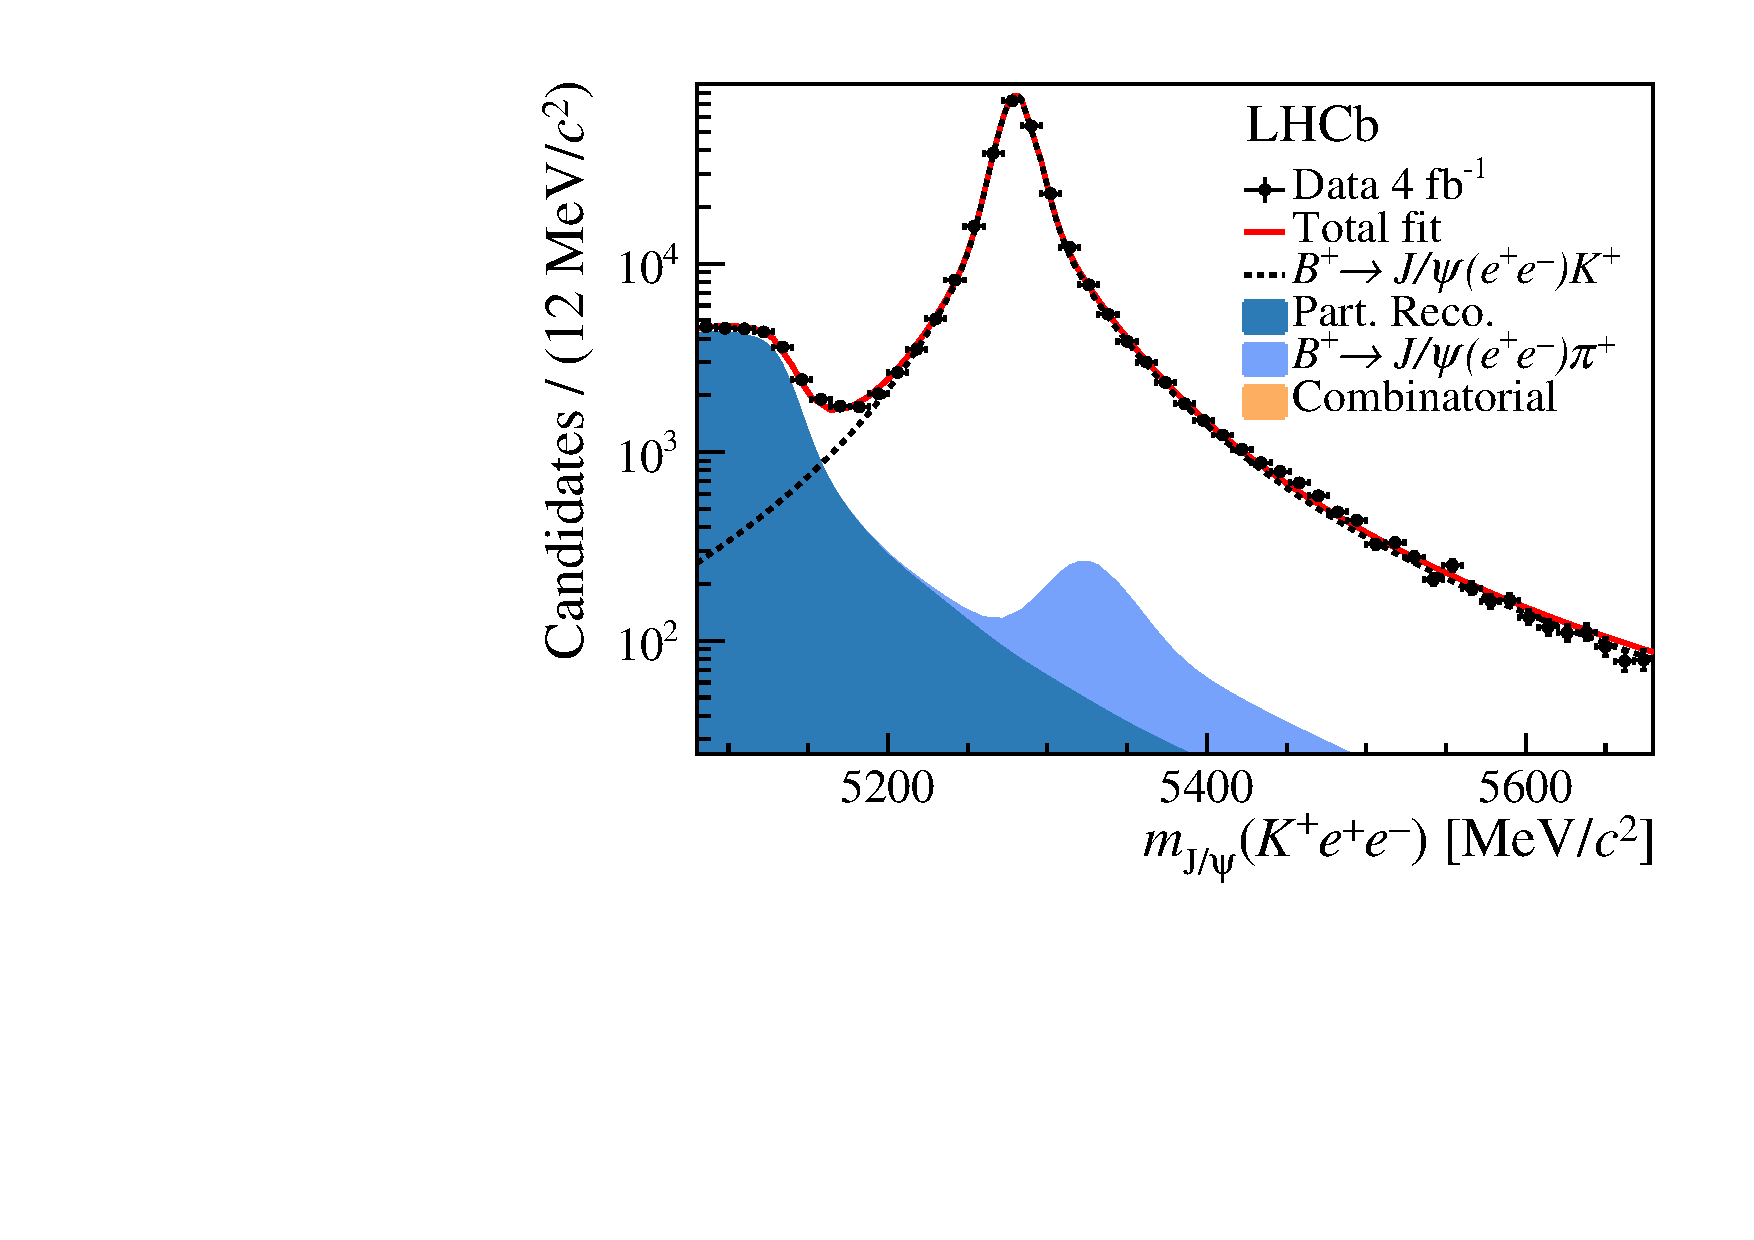
\includegraphics[width=0.45\textwidth]{figures/Fig7d.pdf}
    
    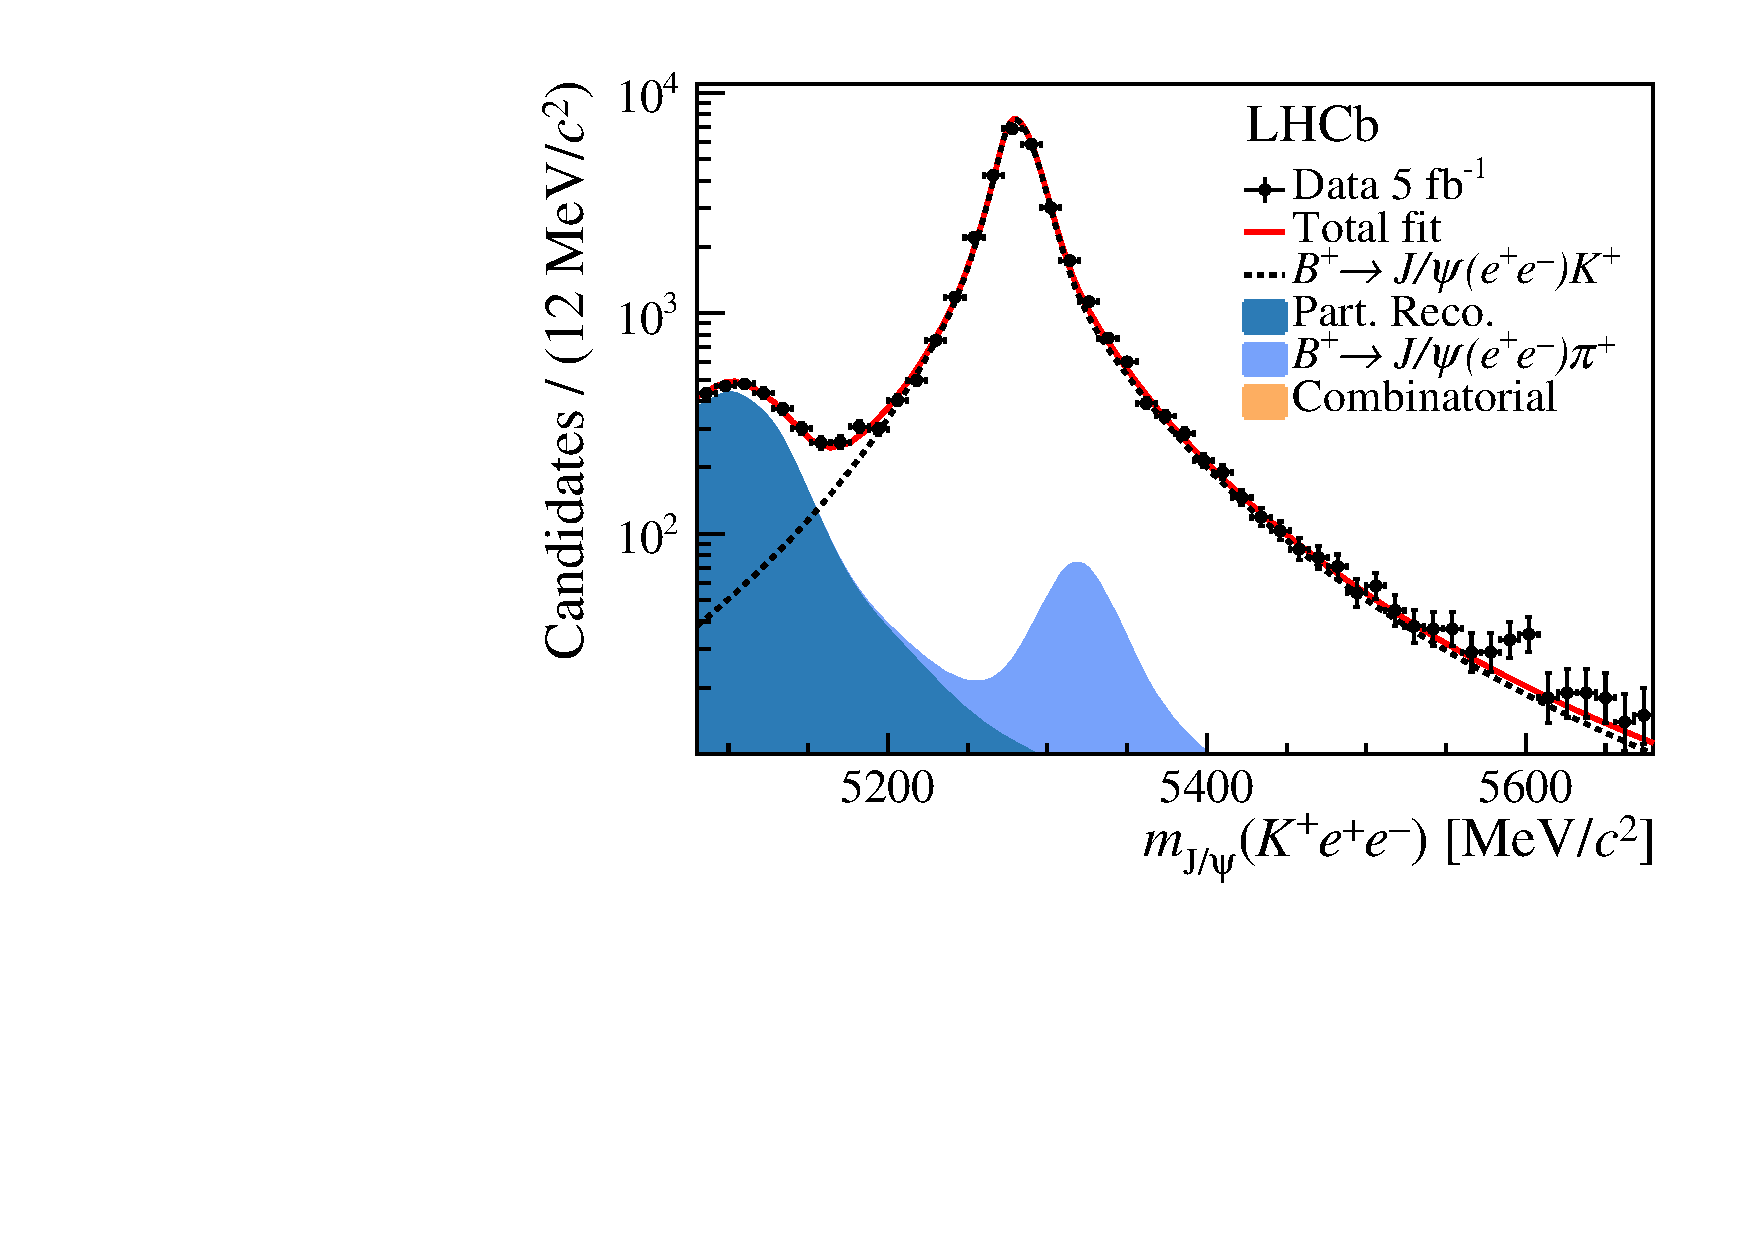
\includegraphics[width=0.45\textwidth]{figures/Fig7e.pdf}
    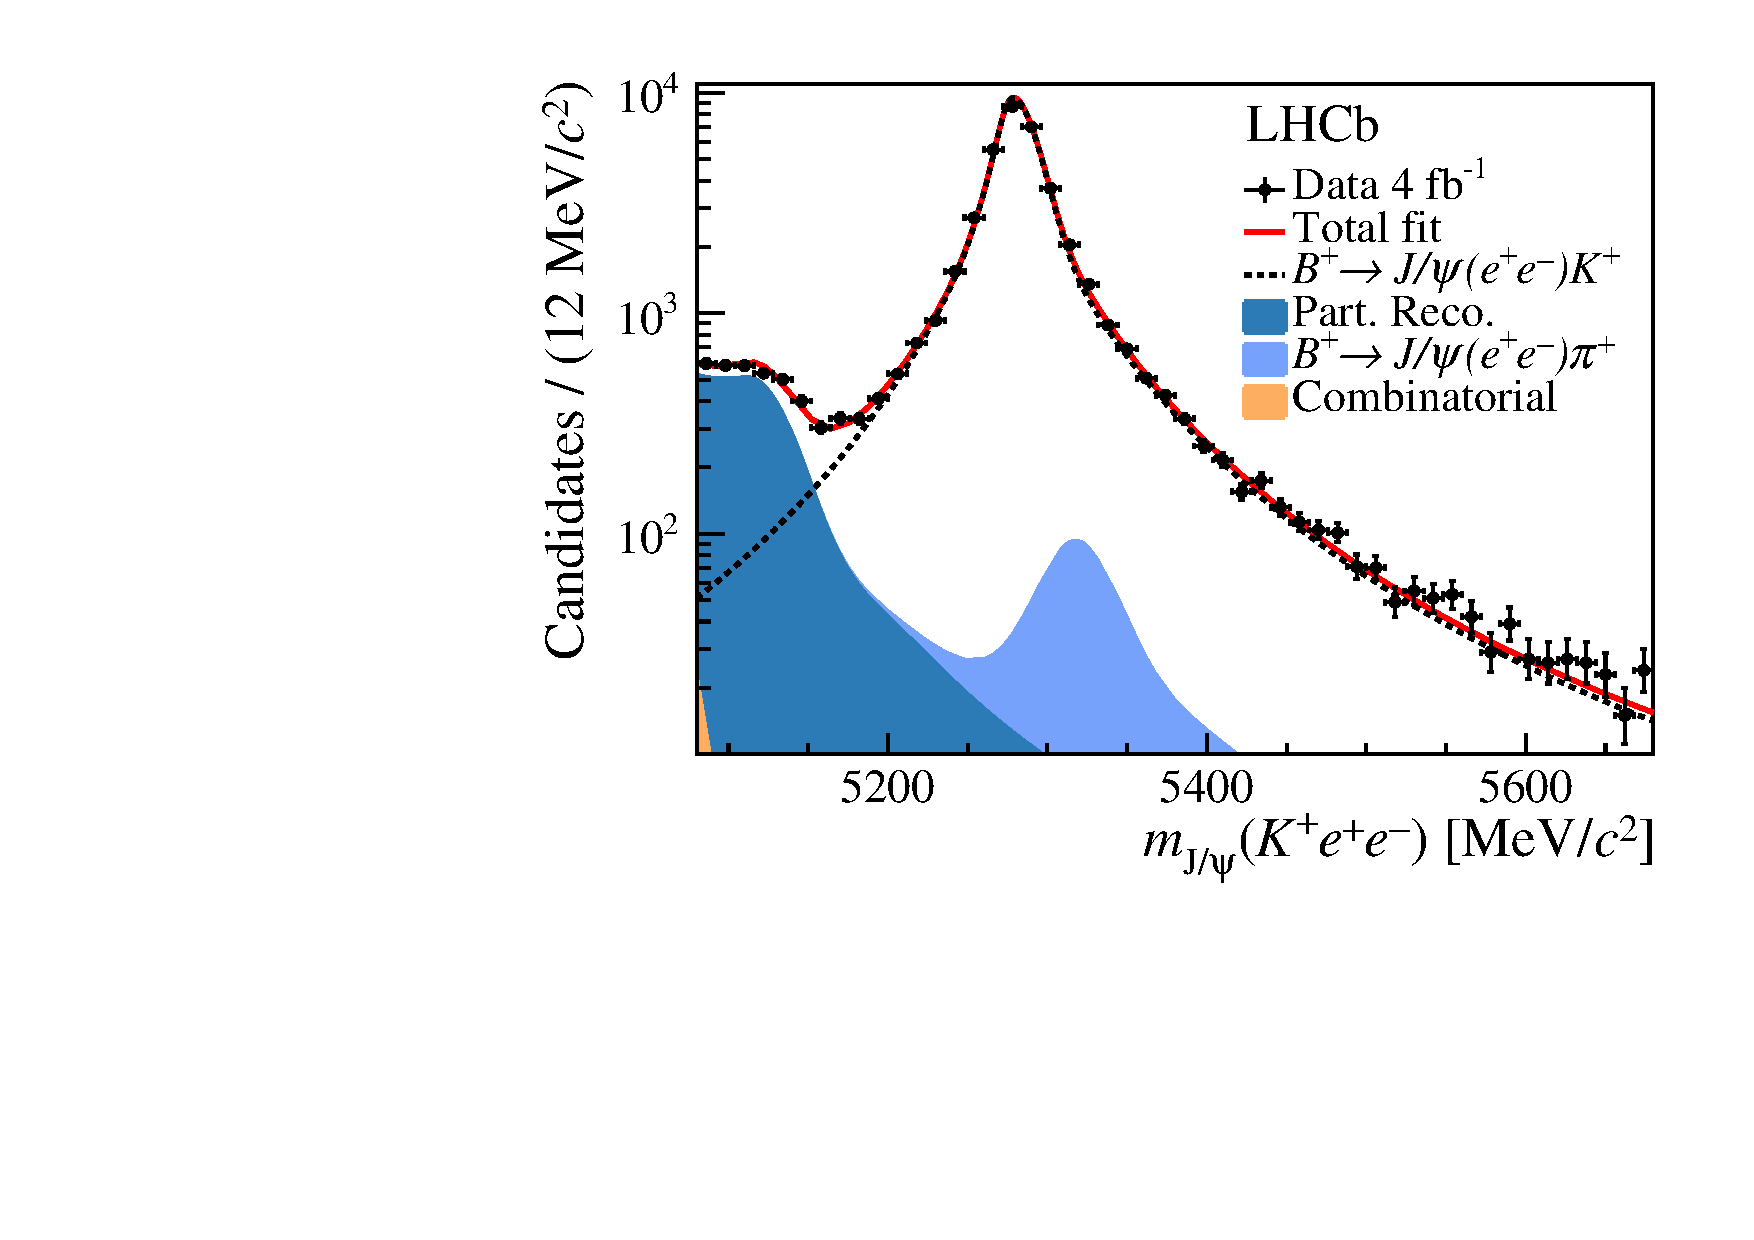
\includegraphics[width=0.45\textwidth]{figures/Fig7f.pdf}
    
    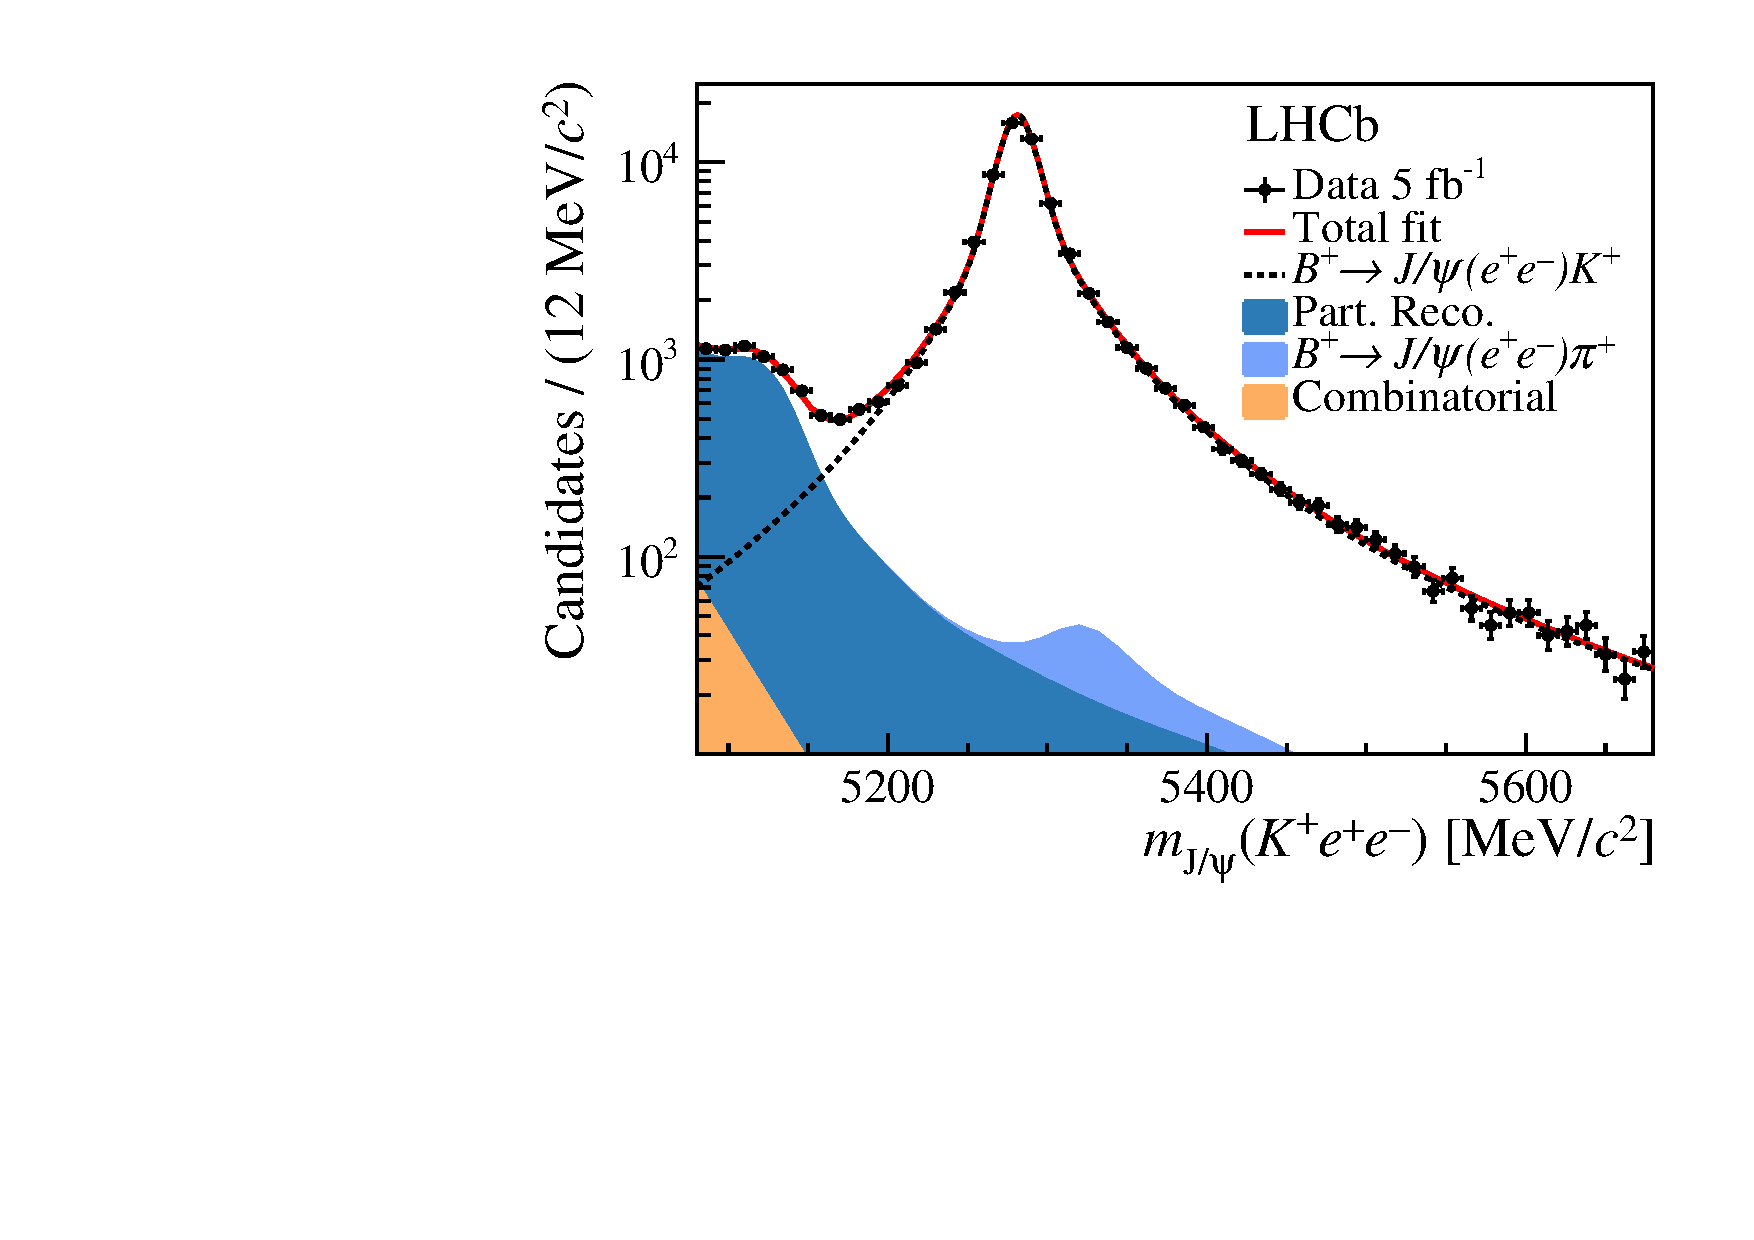
\includegraphics[width=0.45\textwidth]{figures/Fig7g.pdf}
    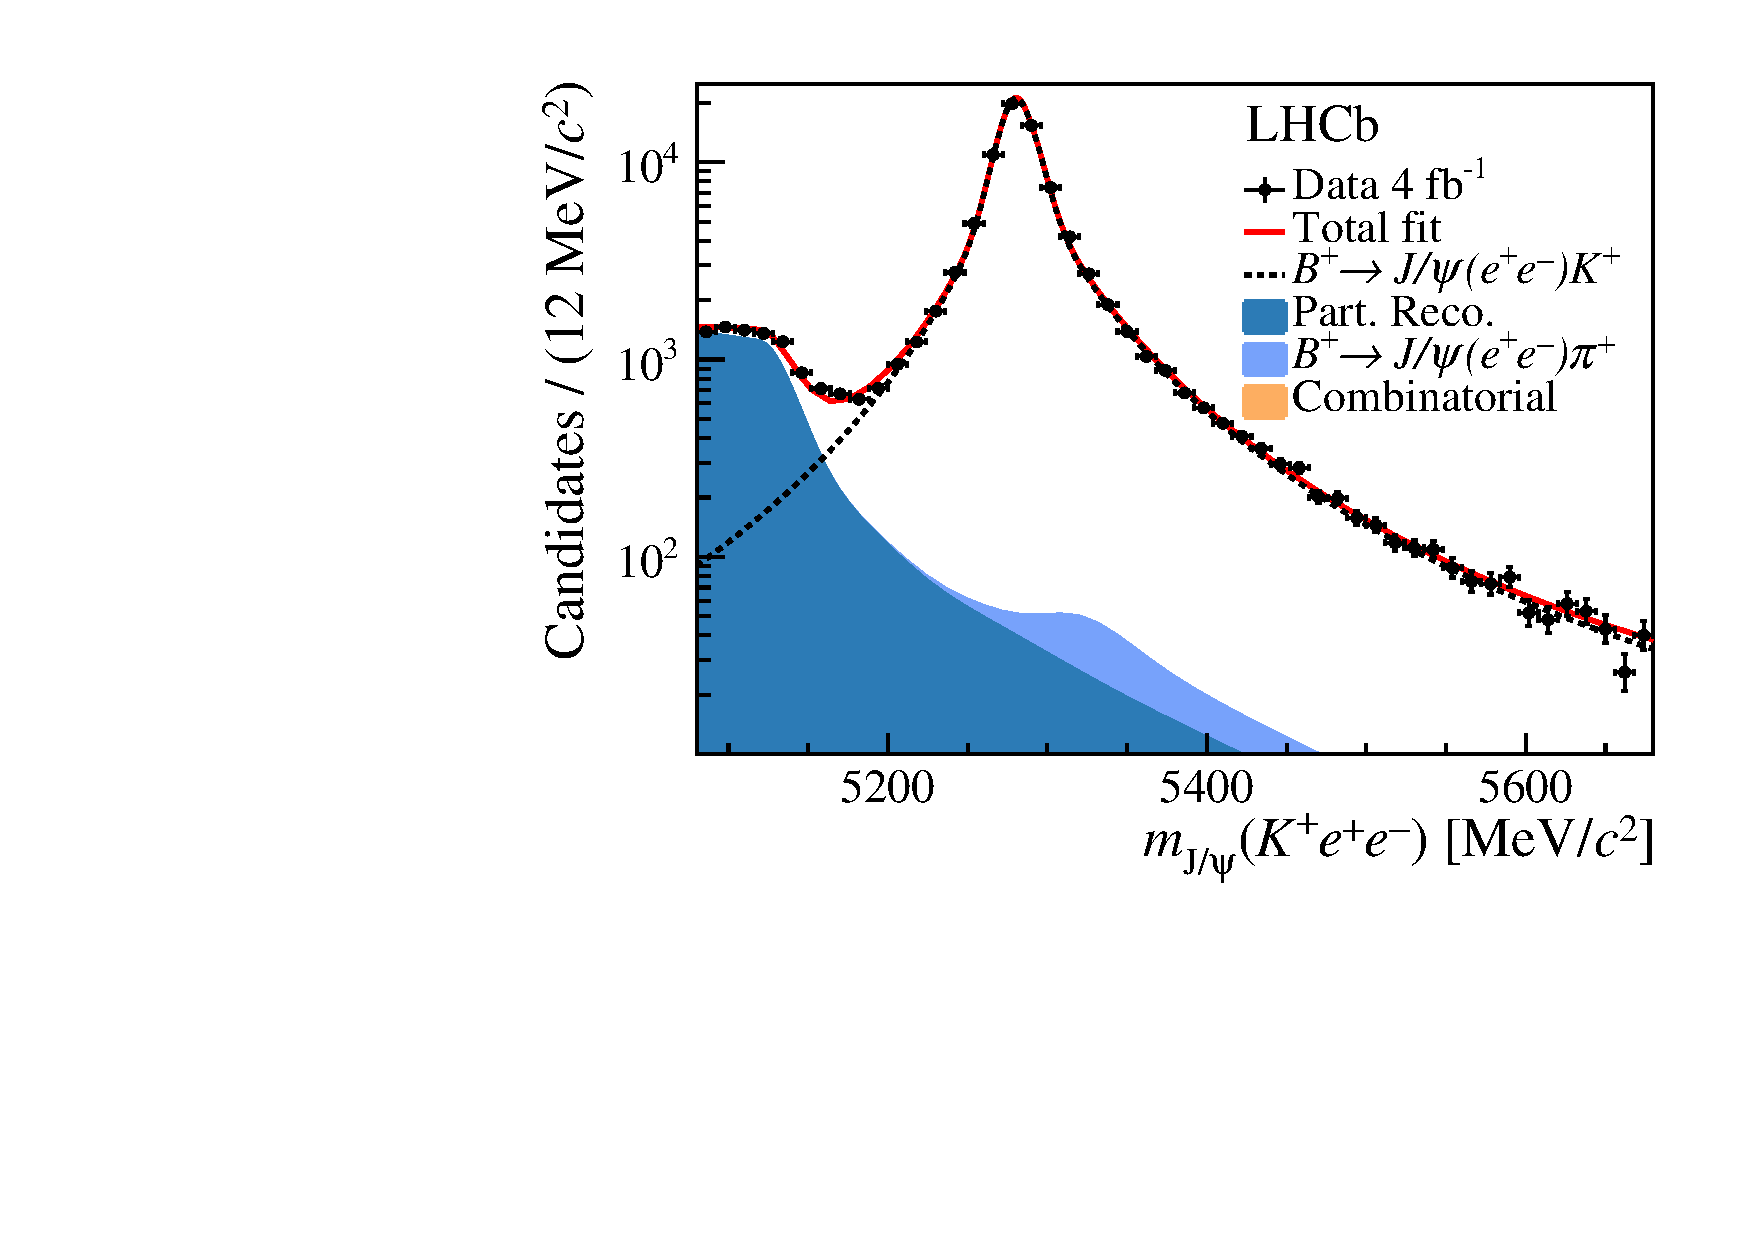
\includegraphics[width=0.45\textwidth]{figures/Fig7h.pdf}
    
    \caption{Candidate invariant mass distributions. Distribution of the invariant mass \mKllconst for resonant candidates in the (left) sample previously analysed~\cite{LHCb-PAPER-2019-009} and (right) the new data sample. The top row shows the fit to the muon modes and the subsequent rows the fits to the electron modes triggered by (second row) one of the electrons, (third row) the kaon and (last row) by other particles in the event. The fit projections are superimposed.
}
    \label{fig:resfits_categories}
\end{figure}


The profile likelihood for the fit to the nonresonant decays is shown in Fig.~\ref{fig:profile_likelihood}. The likelihood is non-Gaussian in the region $\RK>0.95$ due to the comparatively low yield of \BuKee events. 
Following the procedure described in Refs.~\cite{LHCb-PAPER-2019-009, LHCb-PAPER-2017-013}, the p-value is computed by integrating the posterior probability density function for \RK, having folded in the theory uncertainty on the SM prediction, for \RK values larger than the SM  expectation. The corresponding significance in terms of standard deviations is computed using the inverse Gaussian cumulative distribution function for a one-sided conversion.

A test statistic is constructed that is based on the likelihood ratio between two hypotheses with common (null) or different (test) \RK values for the part of the sample analysed previously (7, 8 and part of the 13\tev data) and for the new portion of the 13\tev data. Using pseudoexperiments based on the null hypothesis, the data suggest that the \RK value from the new portion of the data is compatible with that from the previous sample with a p-value of 95\%. Further tests give good compatibility for subsamples of the data corresponding to different trigger categories and magnet polarities.

The departure of the profile likelihood shown in Fig.~\ref{fig:profile_likelihood} from a normal distribution stems from the  definition of \RK. In particular,
in the \RK ratio the denominator is affected by larger statistical uncertainties than the numerator, owing to the larger number of nonresonant muonic signal candidates. However, the intervals of the likelihood distribution are found to be the same when estimated with $1/\RK$ as the fit parameter.


\begin{figure}[!t]
   \begin{center}
      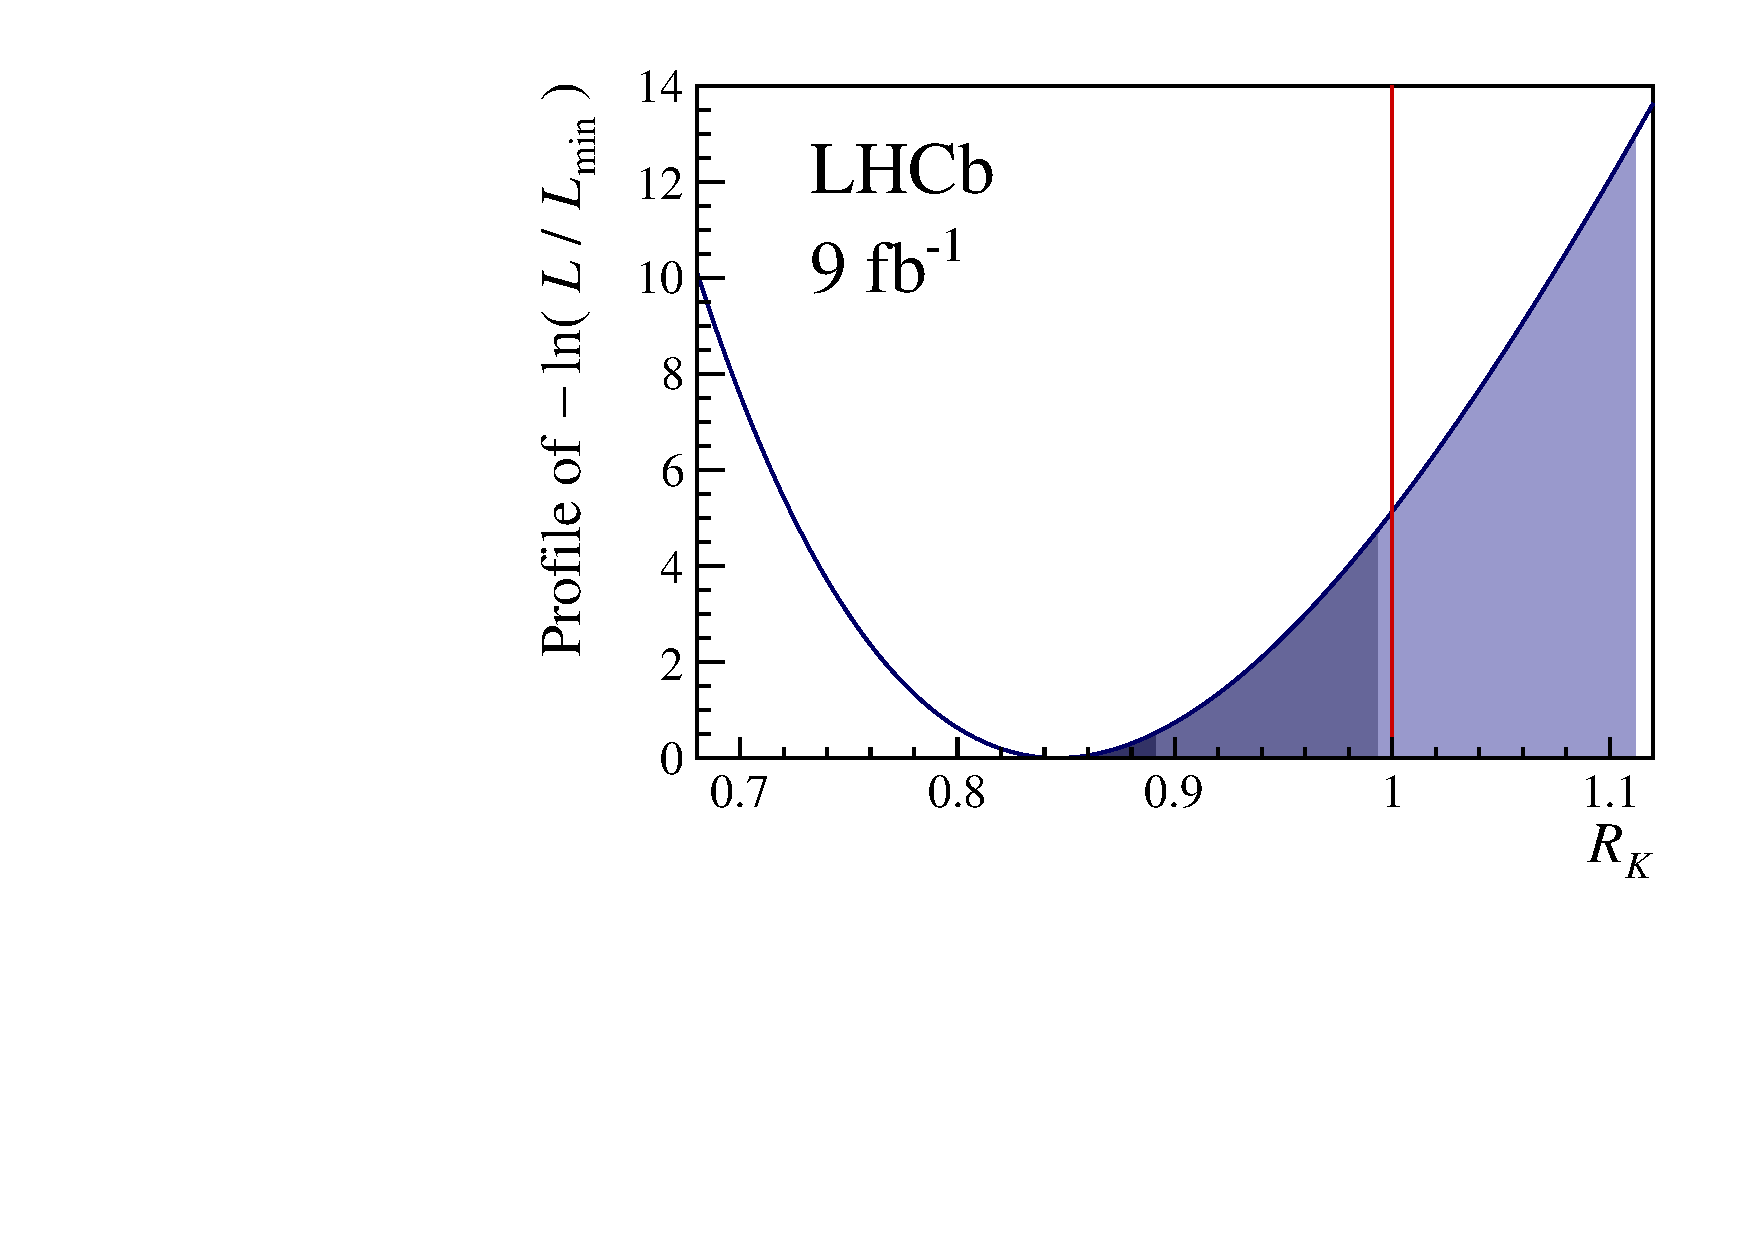
\includegraphics[height=0.25\textheight]{figures/Fig8.pdf}
  \end{center}
     \caption{Likelihood function from the fit to the nonresonant \BuKll candidates profiled as a function of \RK. The extent of the  dark, medium and light blue  regions shows the values allowed for \RK at $1\sigma$, $3\sigma$ and $5\sigma$ levels. The red line indicates the prediction from the SM. }
    \label{fig:profile_likelihood}
\end{figure}



\subsubsection*{Additional cross-checks} 

The \rjpsi single ratio is used to perform a number of additional cross-checks. The distribution of this ratio as a function of the angle between the leptons and the minimum \pt of the leptons is shown in Fig.~\ref{fig:rjpsi_differential1}, together with the spectra expected for the resonant and nonresonant decays.
No significant trend is observed in either \rjpsi distribution. Assuming the deviations observed are genuine mismodelling of the efficiencies, rather than statistical fluctuations, a total shift of \RK at a level less than $0.001$ would be expected due to these effects. This estimate takes into account the spectrum of the relevant variables in the nonresonant decay modes of interest and is compatible with the estimated systematic uncertainties on \RK. Similarly, the variations seen in \rjpsi as a function of all other reconstructed quantities examined are compatible with the systematic uncertainties assigned. In addition, \rjpsi is computed in two-dimensional intervals of reconstructed quantities, as shown in Fig.~\ref{fig:rjpsi_bin}. Again, no significant trend is seen.
 
\begin{figure}[!t]
   \begin{center}
   \begin{overpic}[width=0.45\linewidth,trim={0 0 0 0.5cm}, clip]{figures/Fig9a.pdf}
   \put(50,26){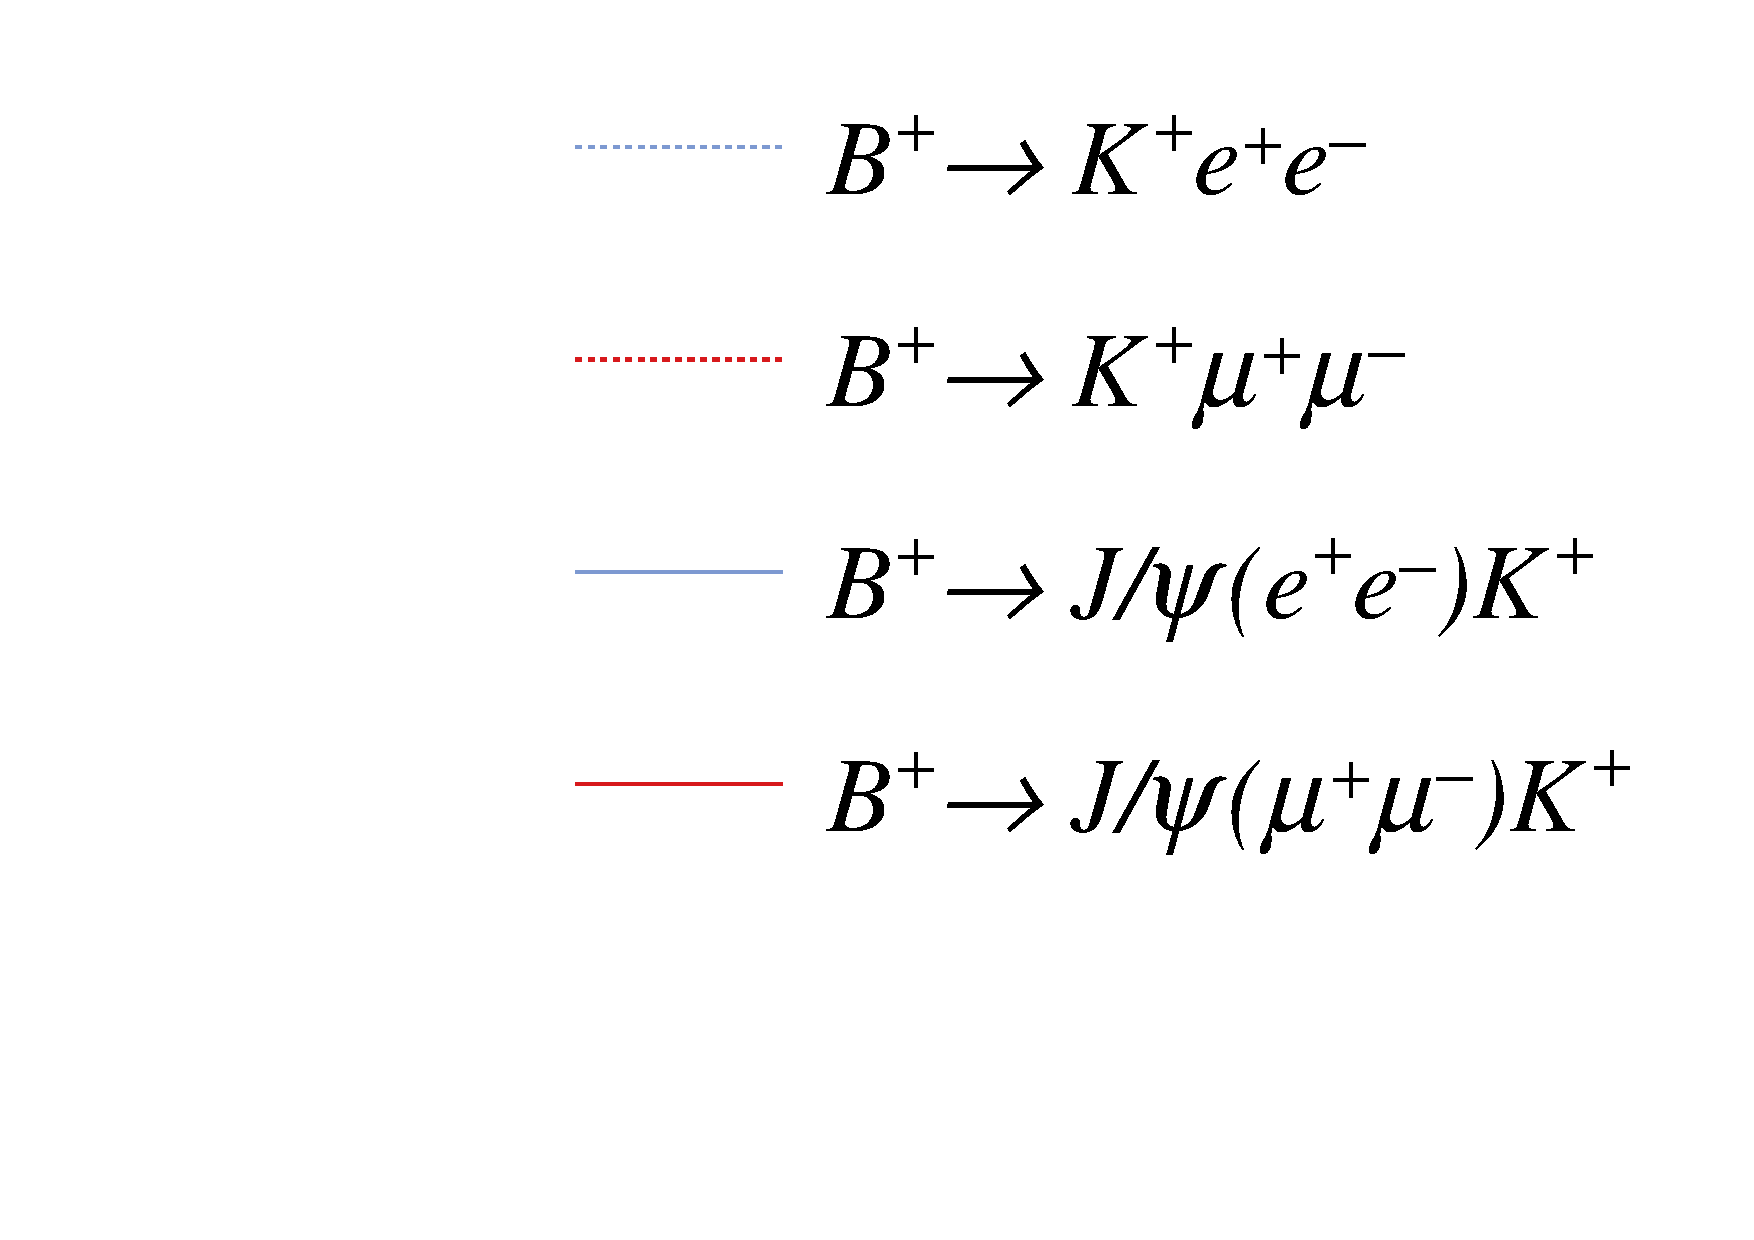
\includegraphics[width=0.2\linewidth]{figures/Fig9e.pdf}}
   \end{overpic}
   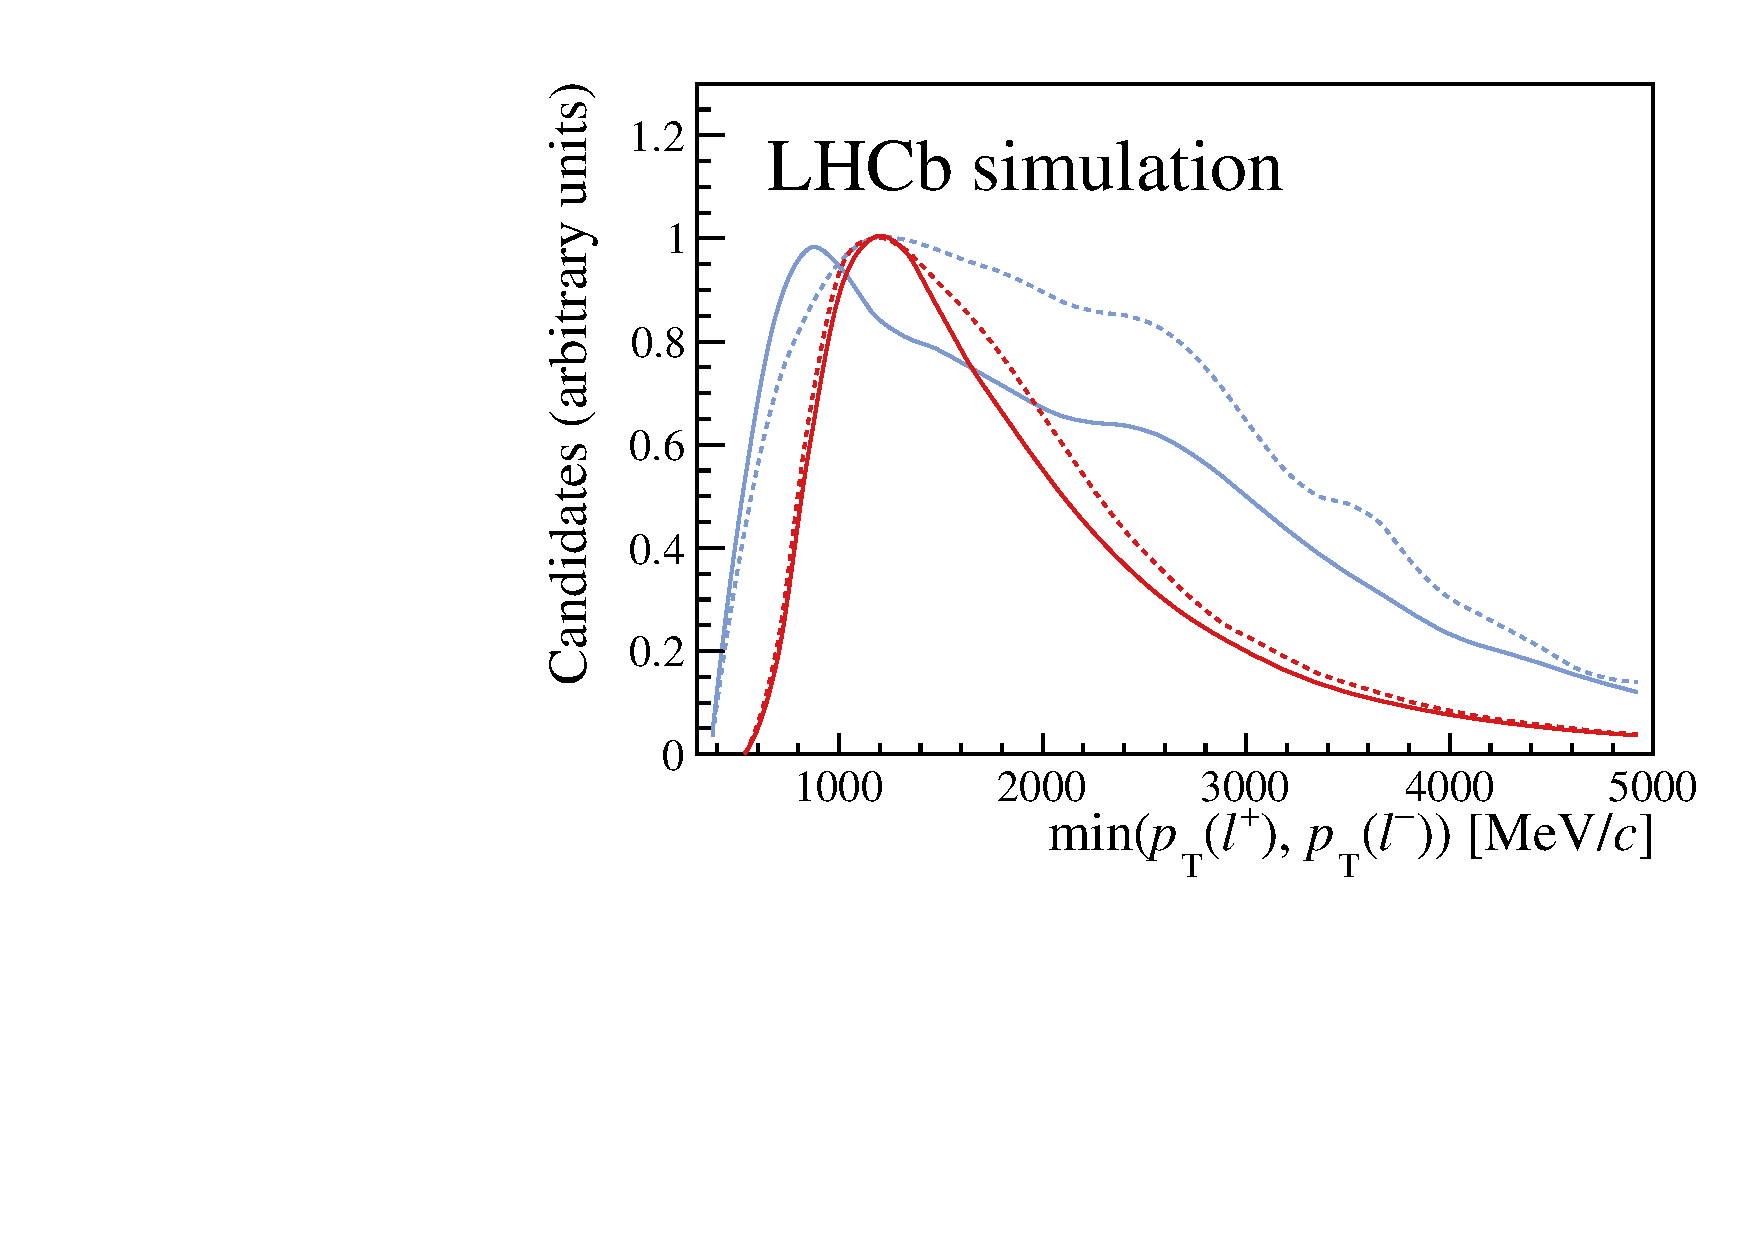
\includegraphics[width=0.45\linewidth,trim={0 0.15cm 0 0}, clip]{figures/Fig9b.pdf}
   
  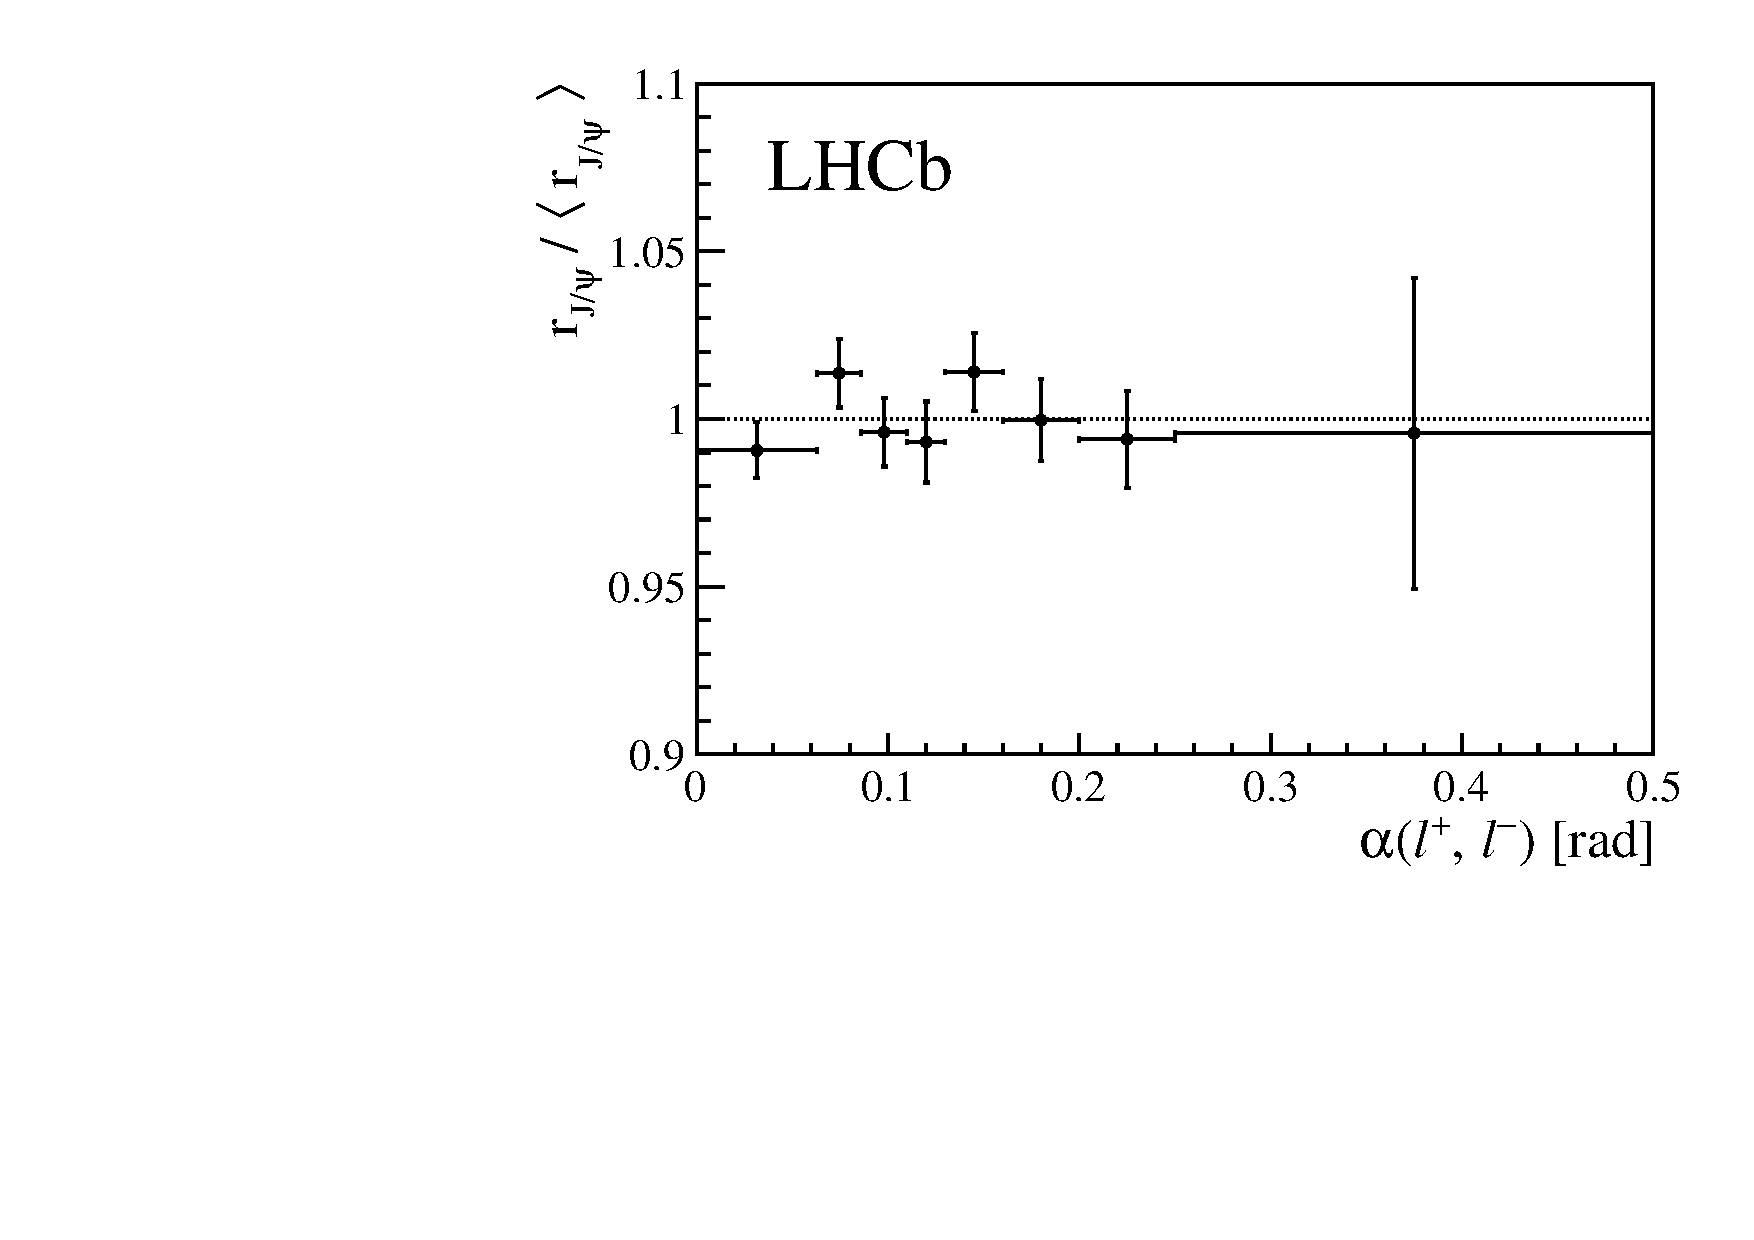
\includegraphics[width=0.45\linewidth,trim={0 0 0 0.5cm}, clip]{figures/Fig9c.pdf}
   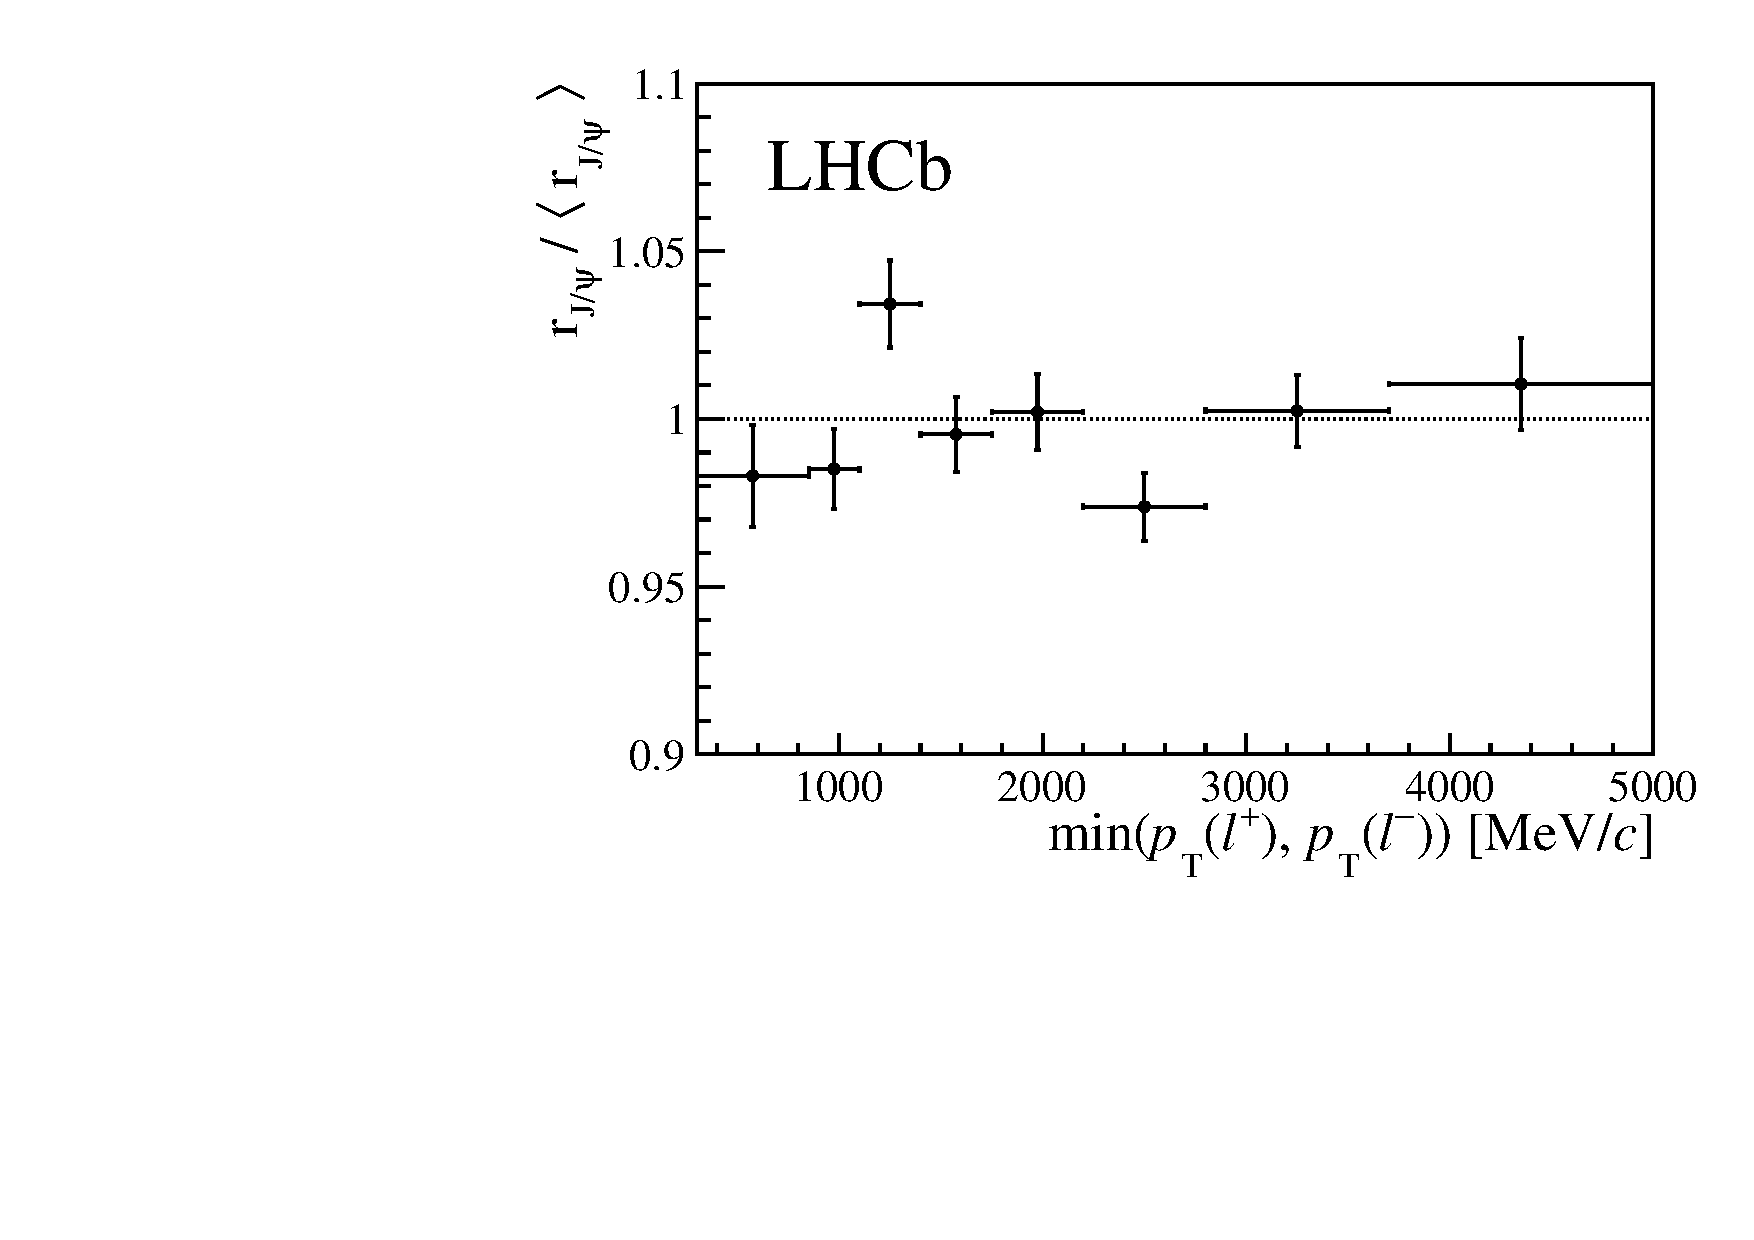
\includegraphics[width=0.45\linewidth,trim={0 0 0 0.5cm}, clip]{figures/Fig9d.pdf}
      \end{center}
     \caption{Differential \rjpsi measurement. (Top) distributions of the reconstructed spectra of (left) the angle between the leptons, and (right) the minimum \pt of the leptons. (Bottom) the single ratio \rjpsi relative to its average value $\left< \rjpsi \right>$ as a function of these variables. In the electron minimum \pt spectra, the structure at 2800\mevc is related to the trigger threshold.}
    \label{fig:rjpsi_differential1}
\end{figure}


\begin{figure}[!htbp]
   \begin{center}
   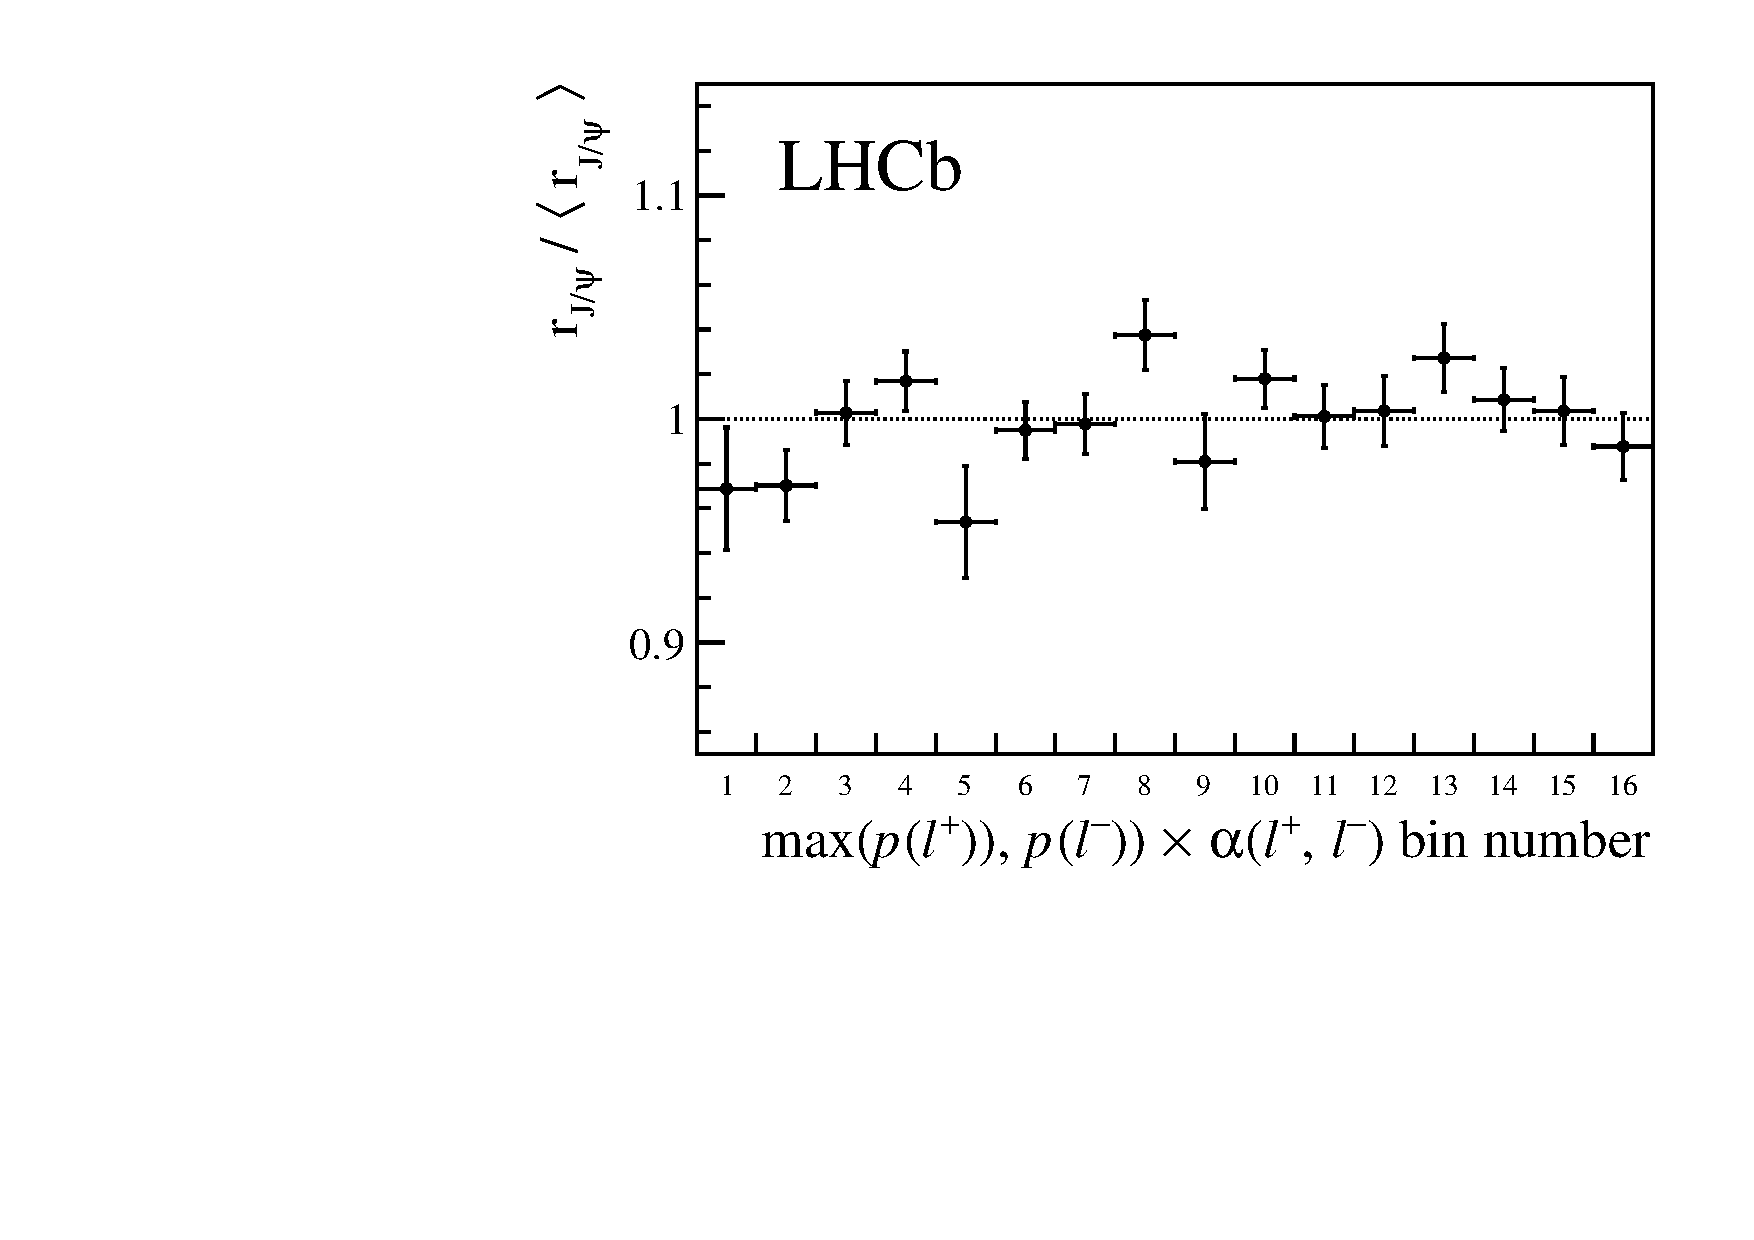
\includegraphics[width=0.45\linewidth]{figures/Fig10a.pdf}
    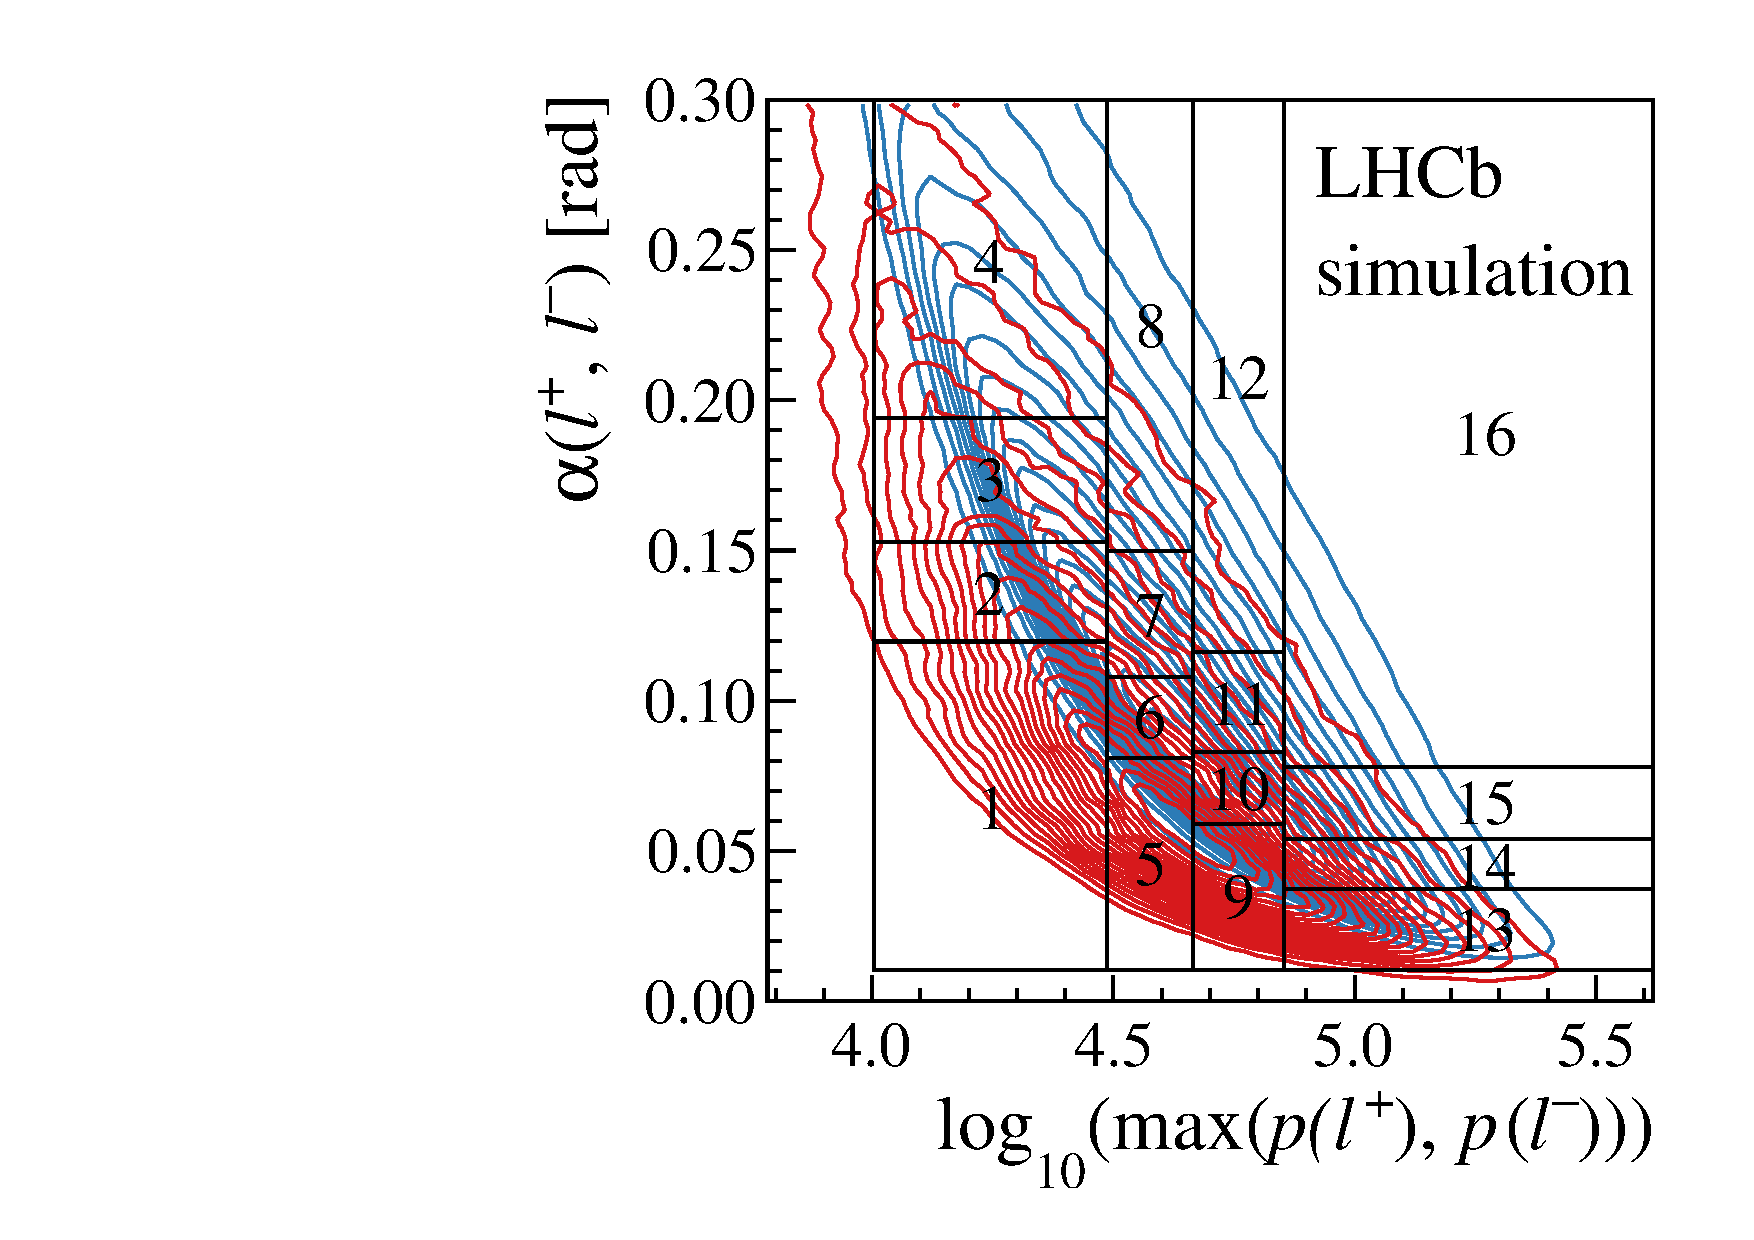
\includegraphics[height=0.32\linewidth]{figures/Fig10b.pdf}
   \end{center}
     \caption{Double differential \rjpsi measurement. (Left) the value of \rjpsi, relative to the average value of \rjpsi, measured in two-dimensional bins of the maximum lepton momentum, $p(l)$, and the opening angle between the two leptons, $\alpha(l^+,l^-)$. (Right) the bin definition in this two-dimensional space together with the
     distribution for \BuKee (\BuJpsiKee) decays depicted as red (blue) contours.}
    \label{fig:rjpsi_bin}
\end{figure}




\subsubsection*{Systematic uncertainties}

The majority of the sources of systematic uncertainty affect the relative efficiencies between nonresonant and resonant decays. These are included in the fit to \RK by allowing the relative efficiency to vary within Gaussian constraints. The width of the constraint is determined by adding the contributions from the different sources in quadrature. Correlations in the systematic uncertainties between different trigger categories and run periods are taken into account. Systematic uncertainties affecting the determination of the signal yield are assessed using pseudoexperiments generated with variations of the fit model. Pseudoexperiments are also used to assess the degree of bias originating from the fitting procedure. The bias is found to be 1\% of the statistical precision, \ie negligible with respect to other sources of systematic uncertainty.

For the nonresonant \BuKee decays, the systematic uncertainties are dominated by the modelling of the signal and background components used in the fit. The effect is at the 1\% level. A significant proportion (0.7\%) of this  uncertainty comes from the limited knowledge of the $K\pi$ spectrum in \BuBdKpiplusee decays. In addition, a 0.2\% systematic uncertainty is assigned for the potential contribution from \BuBdKpipiplusee events. 
A comparable uncertainty to that from the modelling of the signal and background components is induced by the limited sizes of calibration samples. Other sources of systematic uncertainty, such as the calibration of \Bu production kinematics, the trigger calibration and the determination of the particle identification efficiencies, contribute at the few-permille or permille level, depending strongly on the data-taking period and the trigger category. 


% The effect on \RK is at the $\pm0.008$ level. A  comparable uncertainty arises from the limited size of the calibration samples, with negligible contributions from the calibration of \Bu production kinematics and modelling of the selection and particle identification efficiencies. 

The uncertainties on parameters used in the simulation model of the signal decays affect the \qsq distribution and hence the selection efficiency. These uncertainties are propagated to an uncertainty on \RK using predictions from the {\sc{flavio}} software package~\cite{Straub:2018kue} but give rise to a negligible effect. Similarly, the differing \qsq resolution between data and simulation, which alters estimates of the \qsq migration, has negligible impact on the result.




% Comment this in for paper drafts; do not include this in analysis note and conference reports
\extrachap{Acknowledgements}
\addcontentsline{toc}{chapter}{Acknowledgements}

I am forever indebted to my dearest colleagues Edo Liberty, Amir Ingber,
Brian Hentschel, and Aditya Krishnan. This incredible but humble group
of scholars at Pinecone are generous with their time and knowledge,
patiently teaching me what I do not know,
and letting me use them as a sounding board without fail.
Their encouragement throughout the process of writing this manuscript,
too, was the force that drove this work to completion.

I am also grateful to Claudio Lucchese, a dear friend, a co-author,
and a professor of computer science at the Ca' Foscari University of Venice, Italy.
I conceived of the idea for this monograph as I lectured at Ca' Foscari
on the topic of retrieval and ranking, upon Claudio's kind invitation.

I would not be writing these words were it not for
the love, encouragement, and wisdom of Franco Maria Nardini,
of the ISTI CNR in Pisa, Italy. In the mad and often maddening world of research,
Franco is the one knowledgeable and kind soul who
restores my faith in research and guides me as I navigate the landscape.

Finally, there are no words that could possibly convey my deepest gratitude
to my partner, Katherine, for always supporting me and my ambitions;
for showing by example what dedication, tenacity, and grit ought to mean;
and for finding me when I am lost.

%\begin{partbacktext}
\part{Appendices}
\end{partbacktext}

\appendix

\chapter{Collections}
\label{appendix:collections}

\abstract{This appendix gives a description of the vector collections used in experiments
throughout this monograph. These collections demonstrate different operating points in
a typical use-case. For example, some consist of dense vectors, others of sparse vectors;
some have few dimensions and others are in much higher dimensions; some are relatively small
while others contain a large number of points.}

\bigskip

Table~\ref{table:appendix:collections:dense} gives a description of the dense vector collections
used throughout this monograph and summarizes their key statistics.

\begin{table*}[ht]
\caption{Dense collections used in this monograph along with select statistics.}
\scriptsize
\label{table:appendix:collections:dense}
\begin{center}
\begin{sc}
\begin{tabular}{p{5cm}|ccc}
\toprule
Collection & Vector Count & Query Count & Dimensions \\
\midrule
\textsc{GloVe}-$25$~\citep{pennington-etal-2014-glove} & $1.18$M & $10{,}000$ & $25$ \\
\textsc{GloVe}-$50$ & $1.18$M & $10{,}000$ & $50$ \\
\textsc{GloVe}-$100$ & $1.18$M & $10{,}000$ & $100$ \\
\textsc{GloVe}-$200$ & $1.18$M & $10{,}000$ & $200$ \\
\textsc{Deep1b}~\citep{deep1b} & $9.99$M & $10{,}000$ & $96$ \\
\textsc{MS Turing}~\citep{msturingDataset} & $10$M & $100{,}000$ & $100$ \\
\textsc{Sift}~\citep{Lowe2004DistinctiveIF} & $1$M & $10{,}000$ & $128$ \\
\textsc{Gist}~\citep{Oliva2001ModelingTS} & $1$M & $1{,}000$ & $960$ \\
\bottomrule
\end{tabular}
\end{sc}
\end{center}
\end{table*}

In addition to the vector collections above, we convert a few text collections
into vectors using various embedding models. These collections are described in
Table~\ref{table:appendix:collections:text}. Please see~\citep{nguyen2016msmarco} for
a complete description of the MS MARCO v1 collection and~\citep{thakur2021beir} for the others.

\begin{table*}[ht]
\caption{Text collections along with key statistics.
The rightmost two columns report the average number of non-zero
entries in data points and, in parentheses, queries for sparse vector
representations of the collections.}
\scriptsize
\label{table:appendix:collections:text}
\begin{center}
\begin{sc}
\begin{tabular}{c|cc|cc}
\toprule
Collection & Vector Count & Query Count & \splade{} & \esplade{}\\
\midrule
\textsc{MS Marco} Passage& $8.8$M & $6{,}980$ & 127 (49) & 185 (5.9) \\
NQ & $2.68$M & $3{,}452$ & 153 (51) & 212 (8) \\
\textsc{Quora} & $523$K & $10{,}000$ & 68 (65) & 68 (8.9) \\
\textsc{HotpotQA} & $5.23$M & $7{,}405$ & 131 (59) & 125 (13) \\
\textsc{Fever} & $5.42$M & $6{,}666$ & 145 (67) & 140 (8.6) \\
\textsc{DBPedia} & $4.63$M & $400$ & 134 (49) & 131 (5.9) \\
\bottomrule
\end{tabular}
\end{sc}
\end{center}
\end{table*}

When transforming the text collections of Table~\ref{table:appendix:collections:text}
into vectors, we use the following embedding models:
\begin{itemize}
    \item \textsc{AllMiniLM-l6-v2}:\footnote{Available at \url{https://huggingface.co/sentence-transformers/all-MiniLM-L6-v2}}
    Projects text documents into $384$-dimensional dense vectors for retrieval with angular distance.

    \item \textsc{Tas-B}~\citep{tas-b}: A bi-encoder model that was trained using supervision from a cross-encoder and a ColBERT~\citep{colbert2020khattab} model,
    and produces $768$-dimensional dense vectors that are meant for MIPS.
    The checkpoint used in this work is available on HuggingFace.\footnote{Available at \url{https://huggingface.co/sentence-transformers/msmarco-distilbert-base-tas-b}}

    \item \splade{}~\citep{formal2022splade}:\footnote{Pre-trained checkpoint from HuggingFace available at \url{https://huggingface.co/naver/splade-cocondenser-ensembledistil}}
    Produces sparse representations for text.
    The vectors have roughly $30{,}000$ dimensions, where each dimension corresponds
    to a term in the BERT~\citep{devlin2019bert} WordPiece~\citep{wordpiece} vocabulary.
    Non-zero entries in a vector reflect learnt term importance weights.

    \item \esplade{}~\citep{lassance2022sigir}:\footnote{Pre-trained checkpoints for document and
    query encoders were obtained from \url{https://huggingface.co/naver/efficient-splade-V-large-doc} and \url{https://huggingface.co/naver/efficient-splade-V-large-query},
    respectively.}
    This model produces queries that have far fewer non-zero entries than the original
    \splade{} model, but documents that may have a larger number of non-zero entries.
\end{itemize}

\bibliographystyle{abbrvnat}
\bibliography{biblio}


\chapter{Probability Review}
\label{appendix:probability}

\abstract{We briefly review key concepts in probability in this appendix.}

\section{Probability}
We identify a \emph{probability space} denoted by $(\Omega, \mathcal{F}, \probability)$
with an \emph{outcome space}, an \emph{events} set, and a \emph{probability measure}.
The outcome space, $\Omega$, is the set of all
possible outcomes. For example, when flipping a two-sided coin, the outcome
space is simply $\{0, 1\}$. When rolling a six-sided die, it is instead
the set $[6] = \{ 1, 2, \ldots, 6\}$.

The events set $\mathcal{F}$ is a set of subsets of $\Omega$ that
includes $\Omega$ as a member and is closed under complementation and
countable unions. That is, if $E \in \mathcal{F}$,
then we must have that $E^\complement \mathcal{F}$.
Furthermore, the union of countably many events $E_i$'s
in $\mathcal{F}$ is itself in $\mathcal{F}$: $\cup_i E_i \in \mathcal{F}$.
A set $\mathcal{F}$ that satisfies these properties is called a $\sigma$-algebra.

Finally, a function $\probability: \mathcal{F} \rightarrow \mathbb{R}$ is
a probability measure if it satisfies the following conditions: $\probability[\Omega] = 1$;
$\probability[E] \geq 0$ for any event $E \in \mathcal{F}$;
$\probability[E^\complement] = 1 - \probability[E]$; and, finally,
for countably many disjoint events $E_i$'s:
$\probability[\cup_i E_i] = \sum_i \probability[E_i]$.

We should note that, $\probability$ is also known as a ``probability distribution''
or simply a ``distribution.'' The pair $(\Omega, \mathcal{F})$ is called
a \emph{measurable space}, and the elements of $\mathcal{F}$ are
known as a \emph{measurable sets}. The reason they are called ``measurable''
is because they can be ``measured'' with $\probability$: The function
$\probability$ assigns values to them.

In many of the discussions throughout this monograph, we omit the outcome space
and events set because that information is generally clear from context.
However, a more formal treatment of our arguments requires a complete
definition of the probability space.

\section{Random Variables}
A random variable on a measurable space $(\Omega, \mathcal{F})$ is
a measurable function $X: \Omega \rightarrow \mathbb{R}$.
It is measurable in the sense that the \emph{preimage} of any Borel set $B \in \mathcal{B}$
is an event: $X^{-1}(B) = \{ \omega \in \Omega \;|\; X(\omega) \in B \} \in \mathcal{F}$.

A random variable $X$ generates a $\sigma$-algebra that comprises of the preimage
of all Borel sets. It is denoted by $\sigma(X)$
and formally defined as $\sigma(X) = \{ X^{-1}(B) \;|\; B \in \mathcal{B} \}$.

\bigskip

Random variables are typically categorized as discrete or continuous.
$X$ is \emph{discrete} when it maps $\Omega$ to a discrete set.
In that case, its \emph{probability mass function} is defined as $\probability[X = x]$
for some $x$ in its range.
A \emph{continuous} random variable is often associated with a
probability \emph{density} function, $f_X$, such that:
\begin{equation*}
    \probability[a \leq X \leq b] = \int_a^b f_X(x) dx.
\end{equation*}

Consider, for instance, the following probability density function over the real line for
parameters $\mu \in \mathbb{R}$ and $\sigma > 0$:
\begin{equation*}
    f(x) = \frac{1}{\sqrt{2 \pi \sigma^2}} e^{- \frac{(x - \mu)^2}{2\sigma^2}}.
\end{equation*}
A random variable with the density function above is said to follow a Gaussian
distribution with mean $\mu$ and variance $\sigma^2$, denoted by $X \sim \mathcal{N}(\mu, \sigma^2)$.
When $\mu = 0$ and $\sigma^2 = 1$, the resulting distribution is called the standard
Normal distribution.

Gaussian random variables have attractive properties.
For example, the sum of two independent Gaussian random variables is itself a Gaussian variable.
Concretely, $X_1 \sim \mathcal{N}(\mu_1, \sigma_1^2)$ and $X_2 \sim \mathcal{N}(\mu_2, \sigma_2^2)$,
then $X_1 + X_2 \sim \mathcal{N}(\mu_1 + \mu_2, \sigma_1^2 + \sigma_2^2)$.
The sum of the squares of $m$ independent Gaussian random variables, on the other hand,
follows a $\chi^2$-distribution with $m$ degrees of freedom.

\section{Conditional Probability}
Conditional probabilities give us a way to model how the probability of an event changes
in the presence of extra information, such as partial knowledge about a random outcome.
Concretely, if $(\Omega, \mathcal{F}, \probability)$ is a probability space and
$A, B \in \mathcal{F}$ such that $\probability[B] > 0$, then the \emph{conditional
probability} of $A$ given the event $B$ is denoted by $\probability[A \;\lvert\; B]$ and
defined as follows:
\begin{equation*}
    \probability[A \;\lvert\; B] = \frac{\probability[A \cap B]}{\probability[B]}.
\end{equation*}

We use a number of helpful results concerning conditional probabilities
in proofs throughout the monograph. One particularly useful inequality
is what is known as the \emph{union bound} and is stated as follows:
\begin{equation*}
    \probability[\cup_i A_i] \leq \sum_i \probability[A_i].
\end{equation*}

Another fundamental property is the law of total probability.
It states that, for mutually disjoint events $A_i$'s such that
$\Omega = \cup A_i$, the probability of any event $B$ can be expanded
as follows:
\begin{equation*}
    \probability[B] = \sum_i \probability[B \;\lvert\; A_i] \probability[A_i].
\end{equation*}
This is easy to verify: the summand is by definition equal to $\probability[B \cap A_i]$
and, considering the events $(B \cap A_i)$'s are mutually disjoint, their sum
is equal to $\probability[B \cap (\cup A_i)] = \probability[B]$.


\section{Independence}
Another tool that reflects the effect (or lack thereof) of additional knowledge on probabilities
is the concept of \emph{independence}. Two events $A$ and $B$ are said to be
\emph{independent} if $\probability[A \cap B] = \probability[A] \times \probability[B]$.
Equivalently, we say that $A$ is independent of $B$ if and only if
$\probability[A \;\lvert\; B] = \probability[A]$ when $\probability[B] > 0$.

\bigskip

Independence between two random variables is defined similarly but requires a bit more care.
If $X$ and $Y$ are two random variables and $\sigma(X)$ and $\sigma(Y)$ denote
the $\sigma$-algebras generated by them, then $X$ is independent of $Y$ if
all events $A \in \sigma(X)$ and $B \in \sigma(Y)$ are independent.

When a sequence of random variables are \emph{mutually} independent and are drawn
from the same distribution (i.e., have the same probability density function),
we say the random variables are drawn \emph{iid}: independent and identically-distributed.
We stress that \emph{mutual} independence is a stronger restriction than
\emph{pairwise} independence: $m$ events $\{ E_i \}_{i=1}^m$ are mutually independent if
$\probability[\cap_i E_i] = \prod_i \probability[E_i]$.

We typically assume that data and query points are drawn \emph{iid} from some
(unknown) distribution. This is a standard and often necessary assumption
that eases analysis.

\section{Expectation and Variance}

The \emph{expected value} of a discrete random variable $X$ is denoted by $\ev[X]$
and defined as follows:
\begin{equation*}
    \ev[X] = \sum_x x \probability[X = x].
\end{equation*}
When $X$ is continuous, its expected value is based on the following Lebesgue integral:
\begin{equation*}
    \ev[X] = \int_{\Omega} X d \probability.
\end{equation*}
So when a random variable has probability density function $f_X$, its expected value
becomes:
\begin{equation*}
    \ev[X] = \int x f_X(x) dx.
\end{equation*}

For a \emph{nonnegative} random variable $X$, it is sometimes more convenient to
unpack $\ev{X}$ as follows instead:
\begin{equation*}
    \ev[X] = \int_0^\infty \probability[X > x] dx.
\end{equation*}

A fundamental property of expectation is that it is a linear operator.
Formally, $\ev[X + Y] = \ev[X] + \ev[Y]$ for two random variables $X$ and $Y$.
We use this property often in proofs.

We state another important property for independent random variables
that is easy to prove.
If $X$ and $Y$ are independent, then $\ev[XY] = \ev[X]\ev[Y]$.

\bigskip

The \emph{variance} of a random variable is defined as follows:
\begin{equation*}
    \var[X] = \ev\Big[ (X - \ev[X])^2 \Big] = \ev[X]^2 - \ev[X^2].
\end{equation*}
Unlike expectation, variance is not linear unless the random variables involved
are independent. It is also easy to see that $\var[aX] = a^2 \var[X]$ for a
constant $a$.

\section{Central Limit Theorem}
The result known as the Central Limit Theorem is one of the most
useful tools in probability. Informally, it states that the average of \emph{iid}
random variables with finite mean and variance converges to a Gaussian distribution.
There are several variants of this result that extend the claim to, for example,
independent but not identically distributed variables. Below we repeat the formal
result for the \emph{iid} case.

\begin{theorem}
    Let $X_i$'s be a sequence of $n$ \emph{iid} random variables with finite mean $\mu$
    and variance $\sigma^2$. Then, for any $x \in \mathbb{R}$:
    \begin{equation*}
        \lim_{n \rightarrow \infty} \probability \Big[
            \underbrace{\frac{(1/n \sum_{i=1}^n X_i) - \mu}{\sigma^2/n}}_Z \leq x
        \Big] = \int_{-\infty}^x \frac{1}{\sqrt{2 \pi}} e^{-\frac{t^2}{2}} dt,
    \end{equation*}
    implying that $Z \sim \mathcal{N}(0, 1)$.
\end{theorem}

\chapter{Concentration of Measure}
\label{appendix:measure}

\abstract{
By the strong law of large numbers, we know that the average of a sequence
of $m$ \emph{iid} random variables with mean $\mu$ converges to $\mu$ with
probability $1$ as $m$ tends to infinity. But how far is that average from
$\mu$ when $m$ is finite? Concentration inequalities helps us answer that question
quantitatively. This appendix reviews important inequalities that are used
in the proofs and arguments throughout this monograph.
}

\section{Markov's Inequality}

\begin{lemma}
    \label{lemma:appendix:concentration:markov}
    For a nonnegative random variable $X$ and a nonnegative constant $a \geq 0$:
    \begin{equation*}
        \probability[X \geq a] \leq \frac{\ev[X]}{a}.
    \end{equation*}
\end{lemma}
\begin{proof}
    Recall that the expectation of a nonnegative random variable $X$ can be written
    as:
    \begin{equation*}
        \ev[X] = \int_0^\infty \probability[X \geq x] dx.
    \end{equation*}
    Because $\probability[X \geq x]$ is monotonically nonincreasing, we can expand
    the above as follows to complete the proof:
    \begin{equation*}
        \ev[X] \geq \int_0^a \probability[X \geq x] dx \geq \int_0^a \probability[X \geq a] dx = a \probability[X \geq a].
    \end{equation*}
\end{proof}

\section{Chebyshev's Inequality}

\begin{lemma}
    \label{lemma:appendix:concentration:chebyshev}
    For a random variable $X$ and a constant $a > 0$:
    \begin{equation*}
        \probability \Big[ \big\lvert X - \ev[X] \big\rvert \geq a \Big] \leq \frac{\var[X]}{a^2}.
    \end{equation*}
\end{lemma}
\begin{proof}
    \begin{equation*}
        \probability \Big[ \big\lvert X - \ev[X] \big\rvert \geq a \Big] =
        \probability \Big[ \big( X - \ev[X] \big)^2 \geq a^2 \Big] \leq \frac{\var[X]}{a^2},
    \end{equation*}
    where the last step follows by the application of Markov's inequality.
\end{proof}

\begin{lemma}
    Let $\{ X_i \}_{i=1}^n$ be a sequence of iid random variables
    with mean $\mu < \infty$ and variance $\sigma^2 < \infty$. For $\delta \in (0, 1)$,
    with probability $1 - \delta$:
    \begin{equation*}
        \Big\lvert \frac{1}{n} \sum_{i = 1}^n X_i - \mu \Big\rvert \leq \sqrt{\frac{\sigma^2}{\delta n}}.
    \end{equation*}
\end{lemma}
\begin{proof}
    By Lemma~\ref{lemma:appendix:concentration:chebyshev}, for any $a > 0$:
    \begin{equation*}
        \probability \Bigg[ \Big\lvert \frac{1}{n}\sum_{i=1}^n X_i - \mu \Big\rvert \geq a \Bigg]
        \leq \frac{\sigma^2/n}{a^2}.
    \end{equation*}
    Setting the right-hand-side to $\delta$, we obtain:
    \begin{equation*}
        \frac{\sigma^2}{n a^2} = \delta \implies a = \sqrt{\frac{\sigma^2}{\delta n}},
    \end{equation*}
    which completes the proof.
\end{proof}

\section{Chernoff Bounds}

\begin{lemma}
    Let $\{ X_i \}_{i=1}^n$ be independent Bernoulli variables with success probability $p_i$.
    Define $X = \sum_i X_i$ and $\mu = \ev[X] = \sum_i p_i$. Then:
    \begin{equation*}
        \probability \Big[ X > (1 + \delta) \mu \Big] \leq e^{-h(\delta) \mu},
    \end{equation*}
    where,
    \begin{equation*}
        h(t) = (1 + t) \log(1 + t) - t.
    \end{equation*}
\end{lemma}
\begin{proof}
    Using Markov's inequality of Lemma~\ref{lemma:appendix:concentration:markov}
    we can write the following for any $t > 0$:
    \begin{equation*}
        \probability\Big[ X > (1 + \delta)\mu \Big] =
            \probability\Big[ e^{tX} > e^{t(1 + \delta)\mu} \Big] \leq
            \frac{\ev\big[ e^{tX} \big]}{e^{t (1 + \delta) \mu}}.
    \end{equation*}
    Expanding the expectation, we obtain:
    \begin{align*}
        \ev\big[e^{tX}\big] &= \ev\Big[ e^{t \sum_i X_i} \Big] = \ev\Big[ \prod_i e^{tX_i} \Big]
        = \prod_i \ev[e^{tX_i}] \\
        &= \prod_i \Big( p_i e^t + (1 - p_i) \Big) \\
        &= \prod_i \big( 1 + p_i (e^t - 1) \big) \\
        &\leq \prod_i e^{p_i(e^t - 1)} = e^{(e^t - 1)\mu}. && \text{by $(1 + t \leq e^t)$} \\
    \end{align*}
    Putting all this together gives us:
    \begin{equation}
        \label{equation:appendix:concentration:chernoff:proof}
        \probability\Big[ X > (1 + \delta)\mu \Big] \leq 
        \frac{e^{(e^t - 1) \mu}}{e^{t (1 + \delta) \mu}}.
    \end{equation}
    This bound holds for any value $t > 0$, and in particular a value of $t$ that
    minimizes the right-hand-side. To find such a $t$, we may differentiate
    the right-hand-side, set it to $0$, and solve for $t$ to obtain:
    \begin{align*}
        \frac{\mu e^t e^{(e^t - 1) \mu}}{e^{t (1 + \delta) \mu}} &-
        \mu ( 1 + \delta ) \frac{e^{(e^t - 1) \mu}}{e^{t (1 + \delta) \mu}} = 0 \\
        &\implies \mu e^t = \mu (1 + \delta) \\
        &\implies t = \log(1 + \delta).
    \end{align*}
    Substituting $t$ into Equation~(\ref{equation:appendix:concentration:chernoff:proof})
    gives the desired result.
\end{proof}

\section{Hoeffding's Inequality}

We need the following result, known as Hoeffding's Lemma, to present
Hoeffding's inequality.

\begin{lemma}
    \label{lemma:appendix:concentration:hoeffding-lemma}
    Let $X$ be a zero-mean random variable that takes values in $[a, b]$.
    For any $t > 0$:
    \begin{equation*}
        \ev\big[ e^{tX} \big] \leq \exp\Big( \frac{t^2 (b - a)^2}{8} \Big).
    \end{equation*}
\end{lemma}
\begin{proof}
    By convexity of $e^{tx}$ and given $x \in [a, b]$ we have that:
    \begin{equation*}
        e^{tx} \leq \frac{b - x}{b - a} e^{ta} +
            \frac{x - a}{b - a} e^{tb}.
    \end{equation*}
    Taking the expectation of both sides, we arrive at:
    \begin{equation*}
        \ev\Big[e^{tx}\Big] \leq
            \frac{b}{b - a} e^{ta} - \frac{a}{b - a} e^{tb}.
    \end{equation*}
    To conclude the proof, we first write the right-hand-side as
    $\exp(h(t(b - a)))$ where:
    \begin{equation*}
        h(x) = \frac{a}{b - a} x + \log \Big( \frac{b}{b - a} - \frac{a}{b - a} e^x \Big).
    \end{equation*}
    By expanding $h(x)$ using Taylor's theorem, it can be shown that
    $h(x) \leq x^2/8$. That completes the proof.
\end{proof}

We are ready to present Hoeffding's inequality.

\begin{lemma}
    Let $\{ X_i \}_{i=1}^n$ be a sequence of iid random variables
    with finite mean $\mu$ and suppose $X_i \in [a, b]$ almost surely.
    For all $\epsilon > 0$:
    \begin{equation*}
        \probability\Bigg[ \Big\lvert \frac{1}{n} \sum_{i=1}^n X_i - \mu \Big\rvert > \epsilon \Bigg] \leq 2 \exp\Big({-\frac{2n \epsilon^2}{(b - a)^2}}\Big).
    \end{equation*}
\end{lemma}
\begin{proof}
    Let $X = 1/n \sum_i X_i - \mu$. Observe by Markov's inequality that:
    \begin{equation*}
        \probability[X \geq \epsilon] = \probability\Big[ e^{tX} \geq e^{t\epsilon} \Big]
        \leq e^{-t\epsilon} \ev[e^{tX}].
    \end{equation*}
    By independence of $X_i$'s and
    the application of Lemma~\ref{lemma:appendix:concentration:hoeffding-lemma}:
    \begin{align*}
        \ev[e^{tX}] &= \ev \Bigg[ \prod_i e^\frac{t(X_i - \mu)}{n} \Bigg] \\
        &= \prod_i \ev \Big[ e^{\frac{t(X_i-\mu)}{n}} \Big] \\
        &\leq \prod_i \exp\Big( \frac{t^2 (b - a)^2}{8 n^2} \Big) \\
        &= \exp\Big( \frac{t^2 (b - a)^2}{8 n} \Big).
    \end{align*}
    We have shown that:
    \begin{equation*}
        \probability[X \geq \epsilon] \leq \exp\Big( -t \epsilon + \frac{t^2 (b - a)^2}{8 n} \Big).
    \end{equation*}
    That statement holds for all values of $t$ and in particular one that minimizes
    the right-hand-side. Solving for that value of $t$ gives us
    $t = 4n\epsilon / (b - a^2)$, which implies:
    \begin{equation*}
        \probability[X \geq \epsilon] \leq e^{-\frac{2n \epsilon^2}{(b - a)^2}}.
    \end{equation*}
    By a symmetric argument we can bound $\probability[X \leq -\epsilon]$. The claim
    follows by the union bound over the two cases.
\end{proof}

\section{Bennet's Inequality}

\begin{lemma}
    Let $\{ X_i \}_{i=1}^n$ be a sequence of independent random variables with zero mean
    and finite variance $\sigma_i^2$. Assume that $\lvert X_i \rvert \leq a$ almost surely for all $i$. Then:
    \begin{equation*}
        \probability\Big[\sum_i X_i \geq t \Big] \leq 
        \exp \Bigg( -\frac{\sigma^2}{a^2} h\Big( \frac{a t}{\sigma^2} \Big) \Bigg),
    \end{equation*}
    where $h(x) = (1 + x) \log(1 + x) - x$ and $\sigma^2 = \sum_i \sigma_i^2$.
\end{lemma}
\begin{proof}
    As usual, we take advantage of Markov's inequality to write:
    \begin{align*}
        \probability\Big[\sum_i X_i \geq t \Big] &\leq
            e^{-\lambda t} \ev \Big[ e^{\lambda \sum_i X_i} \Big] \\
        &= e^{-\lambda t} \ev \Big[ \prod_i e^{\lambda X_i} \Big] \\
        &= e^{-\lambda t} \prod_i \ev \Big[ e^{\lambda X_i} \Big] \\
    \end{align*}
    Using the Taylor expansion of $e^x$, we obtain:
    \begin{align*}
        \ev \Big[ e^{\lambda X_i} \Big] &= \ev \Big[ \sum_{k=0}^\infty \frac{\lambda^k X_i^k}{k!} \Big] \\
        &= 1 + \sum_{k=2}^\infty \frac{\lambda^k \ev[X_i^2 X_i^{k - 2}]}{k!} \\
        &\leq 1 + \sum_{k=2}^\infty \frac{\lambda^k \sigma_i^2 a^{k-2}}{k!} \\
        &= 1 + \frac{\sigma_i^2}{a^2} \sum_{k=2}^\infty \frac{\lambda^k a^k}{k!} \\
        &= 1 + \frac{\sigma_i^2}{a^2} \big( e^{\lambda a} - 1 - \lambda a \big) \\
        &\leq \exp\Big( \frac{\sigma_i^2}{a^2} \big( e^{\lambda a} - 1 - \lambda a \big) \Big).
    \end{align*}
    Putting it all together:
    \begin{align*}
        \probability\Big[\sum_i X_i \geq t \Big] &\leq
            e^{-\lambda t} \prod_i \exp\Big( \frac{\sigma_i^2}{a^2} \big( e^{\lambda a} - 1 - \lambda a \big) \Big) \\
        &= e^{-\lambda t} \exp\Big( \frac{\sigma^2}{a^2} \big( e^{\lambda a} - 1 - \lambda a \big) \Big).
    \end{align*}
    This inequality holds for all values of $\lambda$, and in particular one that minimizes the
    right-hand-side. Setting the derivative of the right-hand-side to $0$ and solving for $\lambda$
    leads to the desired result.
\end{proof}

\chapter{Linear Algebra Review}
\label{appendix:linear-algebra}

\abstract{
This appendix reviews basic concepts from Linear Algebra that are useful
in digesting the material in this monograph.
}

\section{Inner Product}

Denote by $\mathbb{H}$ a vector space.
An inner product $\langle \cdot, \cdot \rangle: \mathbb{H} \times \mathbb{H} \rightarrow \mathbb{R}$
is a function with the following properties:
\begin{itemize}
    \item $\forall \; u \in \mathbb{H},\; \langle u, u \rangle \geq 0$;
    \item $\forall \; u \in \mathbb{H},\; \langle u, u \rangle = 0 \Leftrightarrow u = 0$;
    \item $\forall \; u, v \in \mathbb{H},\; \langle u, v \rangle = \langle v, u \rangle$; and,
    \item $\forall \; u, v, w \in \mathbb{H}, \textit{ and } \alpha, \beta \in \mathbb{R},\; 
    \langle \alpha u + \beta v, w \rangle = \alpha \langle u, w \rangle + \beta \langle v, w \rangle$.
\end{itemize}

We call $\mathbb{H}$ together with the inner product $\langle \cdot, \cdot \rangle$
an \emph{inner product space}.
As an example, when $\mathbb{H} = \mathbb{R}^d$, given two vectors
$u = \sum_{i=1}^d u_i e_i$ and $v = \sum_{i=1}^d v_i e_i$, where $e_i$'s
are the standard basis vectors, the following is an inner product:
\begin{equation*}
    \langle u, v \rangle = \sum_{i = 1}^d u_i v_i.
\end{equation*}

We say two vectors $u$ and $v$ in an inner product space are \emph{orthogonal}
if their inner product is $0$: $\langle u, v \rangle = 0$.

\section{Norms}

A function $\Phi: \mathbb{H} \rightarrow \mathbb{R}_+$ is a norm on
$\mathbb{H}$ if it has the following properties:
\begin{itemize}
    \item Definiteness: For all $u \in \mathbb{H}$, $\Phi(u) = 0 \Leftrightarrow u = 0$;
    \item Homogeneity: For all $u \in \mathbb{H}$ and $\alpha \in \mathbb{R}$,
        $\Phi(\alpha u) = \lvert \alpha \rvert \Phi(u)$; and,
    \item Triangle inequality: $\forall \; u, v \in \mathbb{H}, \; \Phi(u + v) \leq \Phi(u) + \Phi(v)$.
\end{itemize}

Examples include the absolute value on $\mathbb{R}$,
and the $L_p$ norm (for $p \geq 1$) on $\mathbb{R}^d$ denoted by $\lVert \cdot \rVert_p$
and defined as:
\begin{equation*}
    \lVert u \rVert_p = \Big( \sum_{i=1}^d \lvert u_i \rvert^p \Big)^{\frac{1}{p}}.
\end{equation*}
Instances of $L_p$ include the commonly used $L_1$, $L_2$ (Euclidean),
and $L_\infty$ norms, where $\lVert u \rVert_\infty = \max_i \lvert u_i \rvert$.

Note that, when $\mathbb{H}$ is an inner product space, then
the function $\lVert u \rVert = \sqrt{\langle u, u \rangle}$ is a norm.

\section{Distance}
A norm on a vector space induces a notion of distance between two vectors.
Concretely, if $\mathbb{H}$ is a normed space equipped with $\lVert \cdot \rVert$,
then we define the distance between two vectors $u, v \in \mathbb{H}$ as follows:
\begin{equation*}
    \delta(u, v) = \lVert u - v \rVert.
\end{equation*}

\section{Orthogonal Projection}

\begin{lemma}
    Let $\mathbb{H}$ be an inner product space and suppose $u \in \mathbb{H}$ and $u \neq 0$.
    Any vector $v \in \mathbb{H}$ can be uniquely decomposed along $u$ as:
    \begin{equation*}
        v = v_{\perp} + v_{\parallel},
    \end{equation*}
    such that $\langle v_\perp, v_\parallel \rangle = 0$. Additionally:
    \begin{equation*}
        v_\parallel = \frac{\langle u, v \rangle}{\langle u, u \rangle} u,
    \end{equation*}
    and $v_\perp = v - v_\parallel$.
\end{lemma}
\begin{proof}
    Let $v_\parallel = \alpha u$ and $v_\perp = v - v_\parallel$.
    Because $v_\parallel$ and $v_\perp$ are orthogonal, we deduce that:
    \begin{align*}
        \langle v_\parallel, v_\perp \rangle = 0 \implies
            \langle \alpha u, v_\perp \rangle = 0 \implies
            \langle u, v_\perp \rangle = 0.
    \end{align*}
    That implies:
    \begin{align*}
        \langle v, u \rangle = \alpha \langle u, u \rangle \implies
        \alpha = \frac{\langle u, v \rangle}{\langle u, u \rangle},
    \end{align*}
    so that:
    \begin{equation*}
        v_\parallel = \frac{\langle u, v \rangle}{\langle u, u \rangle} u.
    \end{equation*}

    We prove the uniqueness of the decomposition by contradiction.
    Suppose there exists another decomposition of $v$ to $v_\parallel^\prime + v_\perp^\prime$.
    Then:
    \begin{align*}
        v_\parallel + v_\perp = v_\parallel^\prime + v_\perp^\prime &\implies
        \langle u, v_\parallel + v_\perp \rangle = \langle u,  v_\parallel^\prime + v_\perp^\prime\rangle \\
        &\implies \langle u, v_\parallel \rangle = \langle u,  v_\parallel^\prime \rangle \\
        &\implies \langle u, \alpha u \rangle = \langle u, \beta u \rangle \\
        &\implies \alpha = \beta.
    \end{align*}
    We must therefore also have that $v_\perp = v_\perp^\prime$.
\end{proof}



\addcontentsline{toc}{section}{References}
%\setboolean{inbibliography}{true}
\bibliographystyle{LHCb}
\bibliography{main,standard,LHCb-PAPER,LHCb-CONF,LHCb-DP,LHCb-TDR}

\cleardoublepage
% LHCb collaboration author list
% Data extracted on March 17th, 2021 at 6:21pm for paper reference LHCb-PAPER-2021-004
\centerline
{\large\bf LHCb collaboration}
\begin
{flushleft}
\small
R.~Aaij$^{32}$,
C.~Abell{\'a}n~Beteta$^{50}$,
T.~Ackernley$^{60}$,
B.~Adeva$^{46}$,
M.~Adinolfi$^{54}$,
H.~Afsharnia$^{9}$,
C.A.~Aidala$^{85}$,
S.~Aiola$^{25}$,
Z.~Ajaltouni$^{9}$,
S.~Akar$^{65}$,
J.~Albrecht$^{15}$,
F.~Alessio$^{48}$,
M.~Alexander$^{59}$,
A.~Alfonso~Albero$^{45}$,
Z.~Aliouche$^{62}$,
G.~Alkhazov$^{38}$,
P.~Alvarez~Cartelle$^{55}$,
S.~Amato$^{2}$,
Y.~Amhis$^{11}$,
L.~An$^{48}$,
L.~Anderlini$^{22}$,
A.~Andreianov$^{38}$,
M.~Andreotti$^{21}$,
F.~Archilli$^{17}$,
A.~Artamonov$^{44}$,
M.~Artuso$^{68}$,
K.~Arzymatov$^{42}$,
E.~Aslanides$^{10}$,
M.~Atzeni$^{50}$,
B.~Audurier$^{12}$,
S.~Bachmann$^{17}$,
M.~Bachmayer$^{49}$,
J.J.~Back$^{56}$,
P.~Baladron~Rodriguez$^{46}$,
V.~Balagura$^{12}$,
W.~Baldini$^{21}$,
J.~Baptista~Leite$^{1}$,
R.J.~Barlow$^{62}$,
S.~Barsuk$^{11}$,
W.~Barter$^{61}$,
M.~Bartolini$^{24}$,
F.~Baryshnikov$^{82}$,
J.M.~Basels$^{14}$,
G.~Bassi$^{29}$,
B.~Batsukh$^{68}$,
A.~Battig$^{15}$,
A.~Bay$^{49}$,
M.~Becker$^{15}$,
F.~Bedeschi$^{29}$,
I.~Bediaga$^{1}$,
A.~Beiter$^{68}$,
V.~Belavin$^{42}$,
S.~Belin$^{27}$,
V.~Bellee$^{49}$,
K.~Belous$^{44}$,
I.~Belov$^{40}$,
I.~Belyaev$^{41}$,
G.~Bencivenni$^{23}$,
E.~Ben-Haim$^{13}$,
A.~Berezhnoy$^{40}$,
R.~Bernet$^{50}$,
D.~Berninghoff$^{17}$,
H.C.~Bernstein$^{68}$,
C.~Bertella$^{48}$,
A.~Bertolin$^{28}$,
C.~Betancourt$^{50}$,
F.~Betti$^{48}$,
Ia.~Bezshyiko$^{50}$,
S.~Bhasin$^{54}$,
J.~Bhom$^{35}$,
L.~Bian$^{73}$,
M.S.~Bieker$^{15}$,
S.~Bifani$^{53}$,
P.~Billoir$^{13}$,
M.~Birch$^{61}$,
F.C.R.~Bishop$^{55}$,
A.~Bitadze$^{62}$,
A.~Bizzeti$^{22,k}$,
M.~Bj{\o}rn$^{63}$,
M.P.~Blago$^{48}$,
T.~Blake$^{56}$,
F.~Blanc$^{49}$,
S.~Blusk$^{68}$,
D.~Bobulska$^{59}$,
J.A.~Boelhauve$^{15}$,
O.~Boente~Garcia$^{46}$,
T.~Boettcher$^{64}$,
A.~Boldyrev$^{81}$,
A.~Bondar$^{43}$,
N.~Bondar$^{38,48}$,
S.~Borghi$^{62}$,
M.~Borisyak$^{42}$,
M.~Borsato$^{17}$,
J.T.~Borsuk$^{35}$,
S.A.~Bouchiba$^{49}$,
T.J.V.~Bowcock$^{60}$,
A.~Boyer$^{48}$,
C.~Bozzi$^{21}$,
M.J.~Bradley$^{61}$,
S.~Braun$^{66}$,
A.~Brea~Rodriguez$^{46}$,
M.~Brodski$^{48}$,
J.~Brodzicka$^{35}$,
A.~Brossa~Gonzalo$^{56}$,
D.~Brundu$^{27}$,
A.~Buonaura$^{50}$,
C.~Burr$^{48}$,
A.~Bursche$^{72}$,
A.~Butkevich$^{39}$,
J.S.~Butter$^{32}$,
J.~Buytaert$^{48}$,
W.~Byczynski$^{48}$,
S.~Cadeddu$^{27}$,
H.~Cai$^{73}$,
R.~Calabrese$^{21,f}$,
L.~Calefice$^{15,13}$,
L.~Calero~Diaz$^{23}$,
S.~Cali$^{23}$,
R.~Calladine$^{53}$,
M.~Calvi$^{26,j}$,
M.~Calvo~Gomez$^{84}$,
P.~Camargo~Magalhaes$^{54}$,
A.~Camboni$^{45,84}$,
P.~Campana$^{23}$,
A.F.~Campoverde~Quezada$^{6}$,
S.~Capelli$^{26,j}$,
L.~Capriotti$^{20,d}$,
A.~Carbone$^{20,d}$,
G.~Carboni$^{31}$,
R.~Cardinale$^{24}$,
A.~Cardini$^{27}$,
I.~Carli$^{4}$,
P.~Carniti$^{26,j}$,
L.~Carus$^{14}$,
K.~Carvalho~Akiba$^{32}$,
A.~Casais~Vidal$^{46}$,
G.~Casse$^{60}$,
M.~Cattaneo$^{48}$,
G.~Cavallero$^{48}$,
S.~Celani$^{49}$,
J.~Cerasoli$^{10}$,
A.J.~Chadwick$^{60}$,
M.G.~Chapman$^{54}$,
M.~Charles$^{13}$,
Ph.~Charpentier$^{48}$,
G.~Chatzikonstantinidis$^{53}$,
C.A.~Chavez~Barajas$^{60}$,
M.~Chefdeville$^{8}$,
C.~Chen$^{3}$,
S.~Chen$^{4}$,
A.~Chernov$^{35}$,
V.~Chobanova$^{46}$,
S.~Cholak$^{49}$,
M.~Chrzaszcz$^{35}$,
A.~Chubykin$^{38}$,
V.~Chulikov$^{38}$,
P.~Ciambrone$^{23}$,
M.F.~Cicala$^{56}$,
X.~Cid~Vidal$^{46}$,
G.~Ciezarek$^{48}$,
P.E.L.~Clarke$^{58}$,
M.~Clemencic$^{48}$,
H.V.~Cliff$^{55}$,
J.~Closier$^{48}$,
J.L.~Cobbledick$^{62}$,
V.~Coco$^{48}$,
J.A.B.~Coelho$^{11}$,
J.~Cogan$^{10}$,
E.~Cogneras$^{9}$,
L.~Cojocariu$^{37}$,
P.~Collins$^{48}$,
T.~Colombo$^{48}$,
L.~Congedo$^{19,c}$,
A.~Contu$^{27}$,
N.~Cooke$^{53}$,
G.~Coombs$^{59}$,
G.~Corti$^{48}$,
C.M.~Costa~Sobral$^{56}$,
B.~Couturier$^{48}$,
D.C.~Craik$^{64}$,
J.~Crkovsk\'{a}$^{67}$,
M.~Cruz~Torres$^{1}$,
R.~Currie$^{58}$,
C.L.~Da~Silva$^{67}$,
E.~Dall'Occo$^{15}$,
J.~Dalseno$^{46}$,
C.~D'Ambrosio$^{48}$,
A.~Danilina$^{41}$,
P.~d'Argent$^{48}$,
A.~Davis$^{62}$,
O.~De~Aguiar~Francisco$^{62}$,
K.~De~Bruyn$^{78}$,
S.~De~Capua$^{62}$,
M.~De~Cian$^{49}$,
J.M.~De~Miranda$^{1}$,
L.~De~Paula$^{2}$,
M.~De~Serio$^{19,c}$,
D.~De~Simone$^{50}$,
P.~De~Simone$^{23}$,
J.A.~de~Vries$^{79}$,
C.T.~Dean$^{67}$,
D.~Decamp$^{8}$,
L.~Del~Buono$^{13}$,
B.~Delaney$^{55}$,
H.-P.~Dembinski$^{15}$,
A.~Dendek$^{34}$,
V.~Denysenko$^{50}$,
D.~Derkach$^{81}$,
O.~Deschamps$^{9}$,
F.~Desse$^{11}$,
F.~Dettori$^{27,e}$,
B.~Dey$^{73}$,
P.~Di~Nezza$^{23}$,
S.~Didenko$^{82}$,
L.~Dieste~Maronas$^{46}$,
H.~Dijkstra$^{48}$,
V.~Dobishuk$^{52}$,
A.M.~Donohoe$^{18}$,
F.~Dordei$^{27}$,
A.C.~dos~Reis$^{1}$,
L.~Douglas$^{59}$,
A.~Dovbnya$^{51}$,
A.G.~Downes$^{8}$,
K.~Dreimanis$^{60}$,
M.W.~Dudek$^{35}$,
L.~Dufour$^{48}$,
V.~Duk$^{77}$,
P.~Durante$^{48}$,
J.M.~Durham$^{67}$,
D.~Dutta$^{62}$,
A.~Dziurda$^{35}$,
A.~Dzyuba$^{38}$,
S.~Easo$^{57}$,
U.~Egede$^{69}$,
V.~Egorychev$^{41}$,
S.~Eidelman$^{43,v}$,
S.~Eisenhardt$^{58}$,
S.~Ek-In$^{49}$,
L.~Eklund$^{59,w}$,
S.~Ely$^{68}$,
A.~Ene$^{37}$,
E.~Epple$^{67}$,
S.~Escher$^{14}$,
J.~Eschle$^{50}$,
S.~Esen$^{13}$,
T.~Evans$^{48}$,
A.~Falabella$^{20}$,
J.~Fan$^{3}$,
Y.~Fan$^{6}$,
B.~Fang$^{73}$,
S.~Farry$^{60}$,
D.~Fazzini$^{26,j}$,
M.~F{\'e}o$^{48}$,
A.~Fernandez~Prieto$^{46}$,
J.M.~Fernandez-tenllado~Arribas$^{45}$,
A.D.~Fernez$^{66}$,
F.~Ferrari$^{20,d}$,
L.~Ferreira~Lopes$^{49}$,
F.~Ferreira~Rodrigues$^{2}$,
S.~Ferreres~Sole$^{32}$,
M.~Ferrillo$^{50}$,
M.~Ferro-Luzzi$^{48}$,
S.~Filippov$^{39}$,
R.A.~Fini$^{19}$,
M.~Fiorini$^{21,f}$,
M.~Firlej$^{34}$,
K.M.~Fischer$^{63}$,
D.~Fitzgerald$^{85}$,
C.~Fitzpatrick$^{62}$,
T.~Fiutowski$^{34}$,
F.~Fleuret$^{12}$,
M.~Fontana$^{13}$,
F.~Fontanelli$^{24,h}$,
R.~Forty$^{48}$,
V.~Franco~Lima$^{60}$,
M.~Franco~Sevilla$^{66}$,
M.~Frank$^{48}$,
E.~Franzoso$^{21}$,
G.~Frau$^{17}$,
C.~Frei$^{48}$,
D.A.~Friday$^{59}$,
J.~Fu$^{25}$,
Q.~Fuehring$^{15}$,
W.~Funk$^{48}$,
E.~Gabriel$^{32}$,
T.~Gaintseva$^{42}$,
A.~Gallas~Torreira$^{46}$,
D.~Galli$^{20,d}$,
S.~Gambetta$^{58,48}$,
Y.~Gan$^{3}$,
M.~Gandelman$^{2}$,
P.~Gandini$^{25}$,
Y.~Gao$^{5}$,
M.~Garau$^{27}$,
L.M.~Garcia~Martin$^{56}$,
P.~Garcia~Moreno$^{45}$,
J.~Garc{\'\i}a~Pardi{\~n}as$^{26,j}$,
B.~Garcia~Plana$^{46}$,
F.A.~Garcia~Rosales$^{12}$,
L.~Garrido$^{45}$,
C.~Gaspar$^{48}$,
R.E.~Geertsema$^{32}$,
D.~Gerick$^{17}$,
L.L.~Gerken$^{15}$,
E.~Gersabeck$^{62}$,
M.~Gersabeck$^{62}$,
T.~Gershon$^{56}$,
D.~Gerstel$^{10}$,
Ph.~Ghez$^{8}$,
V.~Gibson$^{55}$,
H.K.~Giemza$^{36}$,
M.~Giovannetti$^{23,p}$,
A.~Giovent{\`u}$^{46}$,
P.~Gironella~Gironell$^{45}$,
L.~Giubega$^{37}$,
C.~Giugliano$^{21,f,48}$,
K.~Gizdov$^{58}$,
E.L.~Gkougkousis$^{48}$,
V.V.~Gligorov$^{13}$,
C.~G{\"o}bel$^{70}$,
E.~Golobardes$^{84}$,
D.~Golubkov$^{41}$,
A.~Golutvin$^{61,82}$,
A.~Gomes$^{1,a}$,
S.~Gomez~Fernandez$^{45}$,
F.~Goncalves~Abrantes$^{63}$,
M.~Goncerz$^{35}$,
G.~Gong$^{3}$,
P.~Gorbounov$^{41}$,
I.V.~Gorelov$^{40}$,
C.~Gotti$^{26}$,
E.~Govorkova$^{48}$,
J.P.~Grabowski$^{17}$,
T.~Grammatico$^{13}$,
L.A.~Granado~Cardoso$^{48}$,
E.~Graug{\'e}s$^{45}$,
E.~Graverini$^{49}$,
G.~Graziani$^{22}$,
A.~Grecu$^{37}$,
L.M.~Greeven$^{32}$,
P.~Griffith$^{21,f}$,
L.~Grillo$^{62}$,
S.~Gromov$^{82}$,
B.R.~Gruberg~Cazon$^{63}$,
C.~Gu$^{3}$,
M.~Guarise$^{21}$,
P. A.~G{\"u}nther$^{17}$,
E.~Gushchin$^{39}$,
A.~Guth$^{14}$,
Y.~Guz$^{44}$,
T.~Gys$^{48}$,
T.~Hadavizadeh$^{69}$,
G.~Haefeli$^{49}$,
C.~Haen$^{48}$,
J.~Haimberger$^{48}$,
T.~Halewood-leagas$^{60}$,
P.M.~Hamilton$^{66}$,
J.P.~Hammerich$^{60}$,
Q.~Han$^{7}$,
X.~Han$^{17}$,
T.H.~Hancock$^{63}$,
S.~Hansmann-Menzemer$^{17}$,
N.~Harnew$^{63}$,
T.~Harrison$^{60}$,
C.~Hasse$^{48}$,
M.~Hatch$^{48}$,
J.~He$^{6,b}$,
M.~Hecker$^{61}$,
K.~Heijhoff$^{32}$,
K.~Heinicke$^{15}$,
A.M.~Hennequin$^{48}$,
K.~Hennessy$^{60}$,
L.~Henry$^{25,47}$,
J.~Heuel$^{14}$,
A.~Hicheur$^{2}$,
D.~Hill$^{49}$,
M.~Hilton$^{62}$,
S.E.~Hollitt$^{15}$,
J.~Hu$^{17}$,
J.~Hu$^{72}$,
W.~Hu$^{7}$,
W.~Huang$^{6}$,
X.~Huang$^{73}$,
W.~Hulsbergen$^{32}$,
R.J.~Hunter$^{56}$,
M.~Hushchyn$^{81}$,
D.~Hutchcroft$^{60}$,
D.~Hynds$^{32}$,
P.~Ibis$^{15}$,
M.~Idzik$^{34}$,
D.~Ilin$^{38}$,
P.~Ilten$^{65}$,
A.~Inglessi$^{38}$,
A.~Ishteev$^{82}$,
K.~Ivshin$^{38}$,
R.~Jacobsson$^{48}$,
S.~Jakobsen$^{48}$,
E.~Jans$^{32}$,
B.K.~Jashal$^{47}$,
A.~Jawahery$^{66}$,
V.~Jevtic$^{15}$,
M.~Jezabek$^{35}$,
F.~Jiang$^{3}$,
M.~John$^{63}$,
D.~Johnson$^{48}$,
C.R.~Jones$^{55}$,
T.P.~Jones$^{56}$,
B.~Jost$^{48}$,
N.~Jurik$^{48}$,
S.~Kandybei$^{51}$,
Y.~Kang$^{3}$,
M.~Karacson$^{48}$,
M.~Karpov$^{81}$,
F.~Keizer$^{48}$,
M.~Kenzie$^{56}$,
T.~Ketel$^{33}$,
B.~Khanji$^{15}$,
A.~Kharisova$^{83}$,
S.~Kholodenko$^{44}$,
T.~Kirn$^{14}$,
V.S.~Kirsebom$^{49}$,
O.~Kitouni$^{64}$,
S.~Klaver$^{32}$,
K.~Klimaszewski$^{36}$,
S.~Koliiev$^{52}$,
A.~Kondybayeva$^{82}$,
A.~Konoplyannikov$^{41}$,
P.~Kopciewicz$^{34}$,
R.~Kopecna$^{17}$,
P.~Koppenburg$^{32}$,
M.~Korolev$^{40}$,
I.~Kostiuk$^{32,52}$,
O.~Kot$^{52}$,
S.~Kotriakhova$^{21,38}$,
P.~Kravchenko$^{38}$,
L.~Kravchuk$^{39}$,
R.D.~Krawczyk$^{48}$,
M.~Kreps$^{56}$,
F.~Kress$^{61}$,
S.~Kretzschmar$^{14}$,
P.~Krokovny$^{43,v}$,
W.~Krupa$^{34}$,
W.~Krzemien$^{36}$,
W.~Kucewicz$^{35,t}$,
M.~Kucharczyk$^{35}$,
V.~Kudryavtsev$^{43,v}$,
H.S.~Kuindersma$^{32,33}$,
G.J.~Kunde$^{67}$,
T.~Kvaratskheliya$^{41}$,
D.~Lacarrere$^{48}$,
G.~Lafferty$^{62}$,
A.~Lai$^{27}$,
A.~Lampis$^{27}$,
D.~Lancierini$^{50}$,
J.J.~Lane$^{62}$,
R.~Lane$^{54}$,
G.~Lanfranchi$^{23}$,
C.~Langenbruch$^{14}$,
J.~Langer$^{15}$,
O.~Lantwin$^{50}$,
T.~Latham$^{56}$,
F.~Lazzari$^{29,q}$,
R.~Le~Gac$^{10}$,
S.H.~Lee$^{85}$,
R.~Lef{\`e}vre$^{9}$,
A.~Leflat$^{40}$,
S.~Legotin$^{82}$,
O.~Leroy$^{10}$,
T.~Lesiak$^{35}$,
B.~Leverington$^{17}$,
H.~Li$^{72}$,
L.~Li$^{63}$,
P.~Li$^{17}$,
S.~Li$^{7}$,
Y.~Li$^{4}$,
Y.~Li$^{4}$,
Z.~Li$^{68}$,
X.~Liang$^{68}$,
T.~Lin$^{61}$,
R.~Lindner$^{48}$,
V.~Lisovskyi$^{15}$,
R.~Litvinov$^{27}$,
G.~Liu$^{72}$,
H.~Liu$^{6}$,
S.~Liu$^{4}$,
X.~Liu$^{3}$,
A.~Loi$^{27}$,
J.~Lomba~Castro$^{46}$,
I.~Longstaff$^{59}$,
J.H.~Lopes$^{2}$,
G.H.~Lovell$^{55}$,
Y.~Lu$^{4}$,
D.~Lucchesi$^{28,l}$,
S.~Luchuk$^{39}$,
M.~Lucio~Martinez$^{32}$,
V.~Lukashenko$^{32}$,
Y.~Luo$^{3}$,
A.~Lupato$^{62}$,
E.~Luppi$^{21,f}$,
O.~Lupton$^{56}$,
A.~Lusiani$^{29,m}$,
X.~Lyu$^{6}$,
L.~Ma$^{4}$,
R.~Ma$^{6}$,
S.~Maccolini$^{20,d}$,
F.~Machefert$^{11}$,
F.~Maciuc$^{37}$,
V.~Macko$^{49}$,
P.~Mackowiak$^{15}$,
S.~Maddrell-Mander$^{54}$,
O.~Madejczyk$^{34}$,
L.R.~Madhan~Mohan$^{54}$,
O.~Maev$^{38}$,
A.~Maevskiy$^{81}$,
D.~Maisuzenko$^{38}$,
M.W.~Majewski$^{34}$,
J.J.~Malczewski$^{35}$,
S.~Malde$^{63}$,
B.~Malecki$^{48}$,
A.~Malinin$^{80}$,
T.~Maltsev$^{43,v}$,
H.~Malygina$^{17}$,
G.~Manca$^{27,e}$,
G.~Mancinelli$^{10}$,
D.~Manuzzi$^{20,d}$,
D.~Marangotto$^{25,i}$,
J.~Maratas$^{9,s}$,
J.F.~Marchand$^{8}$,
U.~Marconi$^{20}$,
S.~Mariani$^{22,g}$,
C.~Marin~Benito$^{48}$,
M.~Marinangeli$^{49}$,
J.~Marks$^{17}$,
A.M.~Marshall$^{54}$,
P.J.~Marshall$^{60}$,
G.~Martellotti$^{30}$,
L.~Martinazzoli$^{48,j}$,
M.~Martinelli$^{26,j}$,
D.~Martinez~Santos$^{46}$,
F.~Martinez~Vidal$^{47}$,
A.~Massafferri$^{1}$,
M.~Materok$^{14}$,
R.~Matev$^{48}$,
A.~Mathad$^{50}$,
Z.~Mathe$^{48}$,
V.~Matiunin$^{41}$,
C.~Matteuzzi$^{26}$,
K.R.~Mattioli$^{85}$,
A.~Mauri$^{32}$,
E.~Maurice$^{12}$,
J.~Mauricio$^{45}$,
M.~Mazurek$^{48}$,
M.~McCann$^{61}$,
L.~Mcconnell$^{18}$,
T.H.~Mcgrath$^{62}$,
A.~McNab$^{62}$,
R.~McNulty$^{18}$,
J.V.~Mead$^{60}$,
B.~Meadows$^{65}$,
C.~Meaux$^{10}$,
G.~Meier$^{15}$,
N.~Meinert$^{76}$,
D.~Melnychuk$^{36}$,
S.~Meloni$^{26,j}$,
M.~Merk$^{32,79}$,
A.~Merli$^{25}$,
L.~Meyer~Garcia$^{2}$,
M.~Mikhasenko$^{48}$,
D.A.~Milanes$^{74}$,
E.~Millard$^{56}$,
M.~Milovanovic$^{48}$,
M.-N.~Minard$^{8}$,
A.~Minotti$^{21}$,
L.~Minzoni$^{21,f}$,
S.E.~Mitchell$^{58}$,
B.~Mitreska$^{62}$,
D.S.~Mitzel$^{48}$,
A.~M{\"o}dden~$^{15}$,
R.A.~Mohammed$^{63}$,
R.D.~Moise$^{61}$,
T.~Momb{\"a}cher$^{15}$,
I.A.~Monroy$^{74}$,
S.~Monteil$^{9}$,
M.~Morandin$^{28}$,
G.~Morello$^{23}$,
M.J.~Morello$^{29,m}$,
J.~Moron$^{34}$,
A.B.~Morris$^{75}$,
A.G.~Morris$^{56}$,
R.~Mountain$^{68}$,
H.~Mu$^{3}$,
F.~Muheim$^{58,48}$,
M.~Mulder$^{48}$,
D.~M{\"u}ller$^{48}$,
K.~M{\"u}ller$^{50}$,
C.H.~Murphy$^{63}$,
D.~Murray$^{62}$,
P.~Muzzetto$^{27,48}$,
P.~Naik$^{54}$,
T.~Nakada$^{49}$,
R.~Nandakumar$^{57}$,
T.~Nanut$^{49}$,
I.~Nasteva$^{2}$,
M.~Needham$^{58}$,
I.~Neri$^{21}$,
N.~Neri$^{25,i}$,
S.~Neubert$^{75}$,
N.~Neufeld$^{48}$,
R.~Newcombe$^{61}$,
T.D.~Nguyen$^{49}$,
C.~Nguyen-Mau$^{49,x}$,
E.M.~Niel$^{11}$,
S.~Nieswand$^{14}$,
N.~Nikitin$^{40}$,
N.S.~Nolte$^{15}$,
C.~Nunez$^{85}$,
A.~Oblakowska-Mucha$^{34}$,
V.~Obraztsov$^{44}$,
D.P.~O'Hanlon$^{54}$,
R.~Oldeman$^{27,e}$,
M.E.~Olivares$^{68}$,
C.J.G.~Onderwater$^{78}$,
A.~Ossowska$^{35}$,
J.M.~Otalora~Goicochea$^{2}$,
T.~Ovsiannikova$^{41}$,
P.~Owen$^{50}$,
A.~Oyanguren$^{47}$,
B.~Pagare$^{56}$,
P.R.~Pais$^{48}$,
T.~Pajero$^{63}$,
A.~Palano$^{19}$,
M.~Palutan$^{23}$,
Y.~Pan$^{62}$,
G.~Panshin$^{83}$,
A.~Papanestis$^{57}$,
M.~Pappagallo$^{19,c}$,
L.L.~Pappalardo$^{21,f}$,
C.~Pappenheimer$^{65}$,
W.~Parker$^{66}$,
C.~Parkes$^{62}$,
C.J.~Parkinson$^{46}$,
B.~Passalacqua$^{21}$,
G.~Passaleva$^{22}$,
A.~Pastore$^{19}$,
M.~Patel$^{61}$,
C.~Patrignani$^{20,d}$,
C.J.~Pawley$^{79}$,
A.~Pearce$^{48}$,
A.~Pellegrino$^{32}$,
M.~Pepe~Altarelli$^{48}$,
S.~Perazzini$^{20}$,
D.~Pereima$^{41}$,
P.~Perret$^{9}$,
M.~Petric$^{59,48}$,
K.~Petridis$^{54}$,
A.~Petrolini$^{24,h}$,
A.~Petrov$^{80}$,
S.~Petrucci$^{58}$,
M.~Petruzzo$^{25}$,
T.T.H.~Pham$^{68}$,
A.~Philippov$^{42}$,
L.~Pica$^{29,n}$,
M.~Piccini$^{77}$,
B.~Pietrzyk$^{8}$,
G.~Pietrzyk$^{49}$,
M.~Pili$^{63}$,
D.~Pinci$^{30}$,
F.~Pisani$^{48}$,
Resmi ~P.K$^{10}$,
V.~Placinta$^{37}$,
J.~Plews$^{53}$,
M.~Plo~Casasus$^{46}$,
F.~Polci$^{13}$,
M.~Poli~Lener$^{23}$,
M.~Poliakova$^{68}$,
A.~Poluektov$^{10}$,
N.~Polukhina$^{82,u}$,
I.~Polyakov$^{68}$,
E.~Polycarpo$^{2}$,
G.J.~Pomery$^{54}$,
S.~Ponce$^{48}$,
D.~Popov$^{6,48}$,
S.~Popov$^{42}$,
S.~Poslavskii$^{44}$,
K.~Prasanth$^{35}$,
L.~Promberger$^{48}$,
C.~Prouve$^{46}$,
V.~Pugatch$^{52}$,
H.~Pullen$^{63}$,
G.~Punzi$^{29,n}$,
W.~Qian$^{6}$,
J.~Qin$^{6}$,
R.~Quagliani$^{13}$,
B.~Quintana$^{8}$,
N.V.~Raab$^{18}$,
R.I.~Rabadan~Trejo$^{10}$,
B.~Rachwal$^{34}$,
J.H.~Rademacker$^{54}$,
M.~Rama$^{29}$,
M.~Ramos~Pernas$^{56}$,
M.S.~Rangel$^{2}$,
F.~Ratnikov$^{42,81}$,
G.~Raven$^{33}$,
M.~Reboud$^{8}$,
F.~Redi$^{49}$,
F.~Reiss$^{62}$,
C.~Remon~Alepuz$^{47}$,
Z.~Ren$^{3}$,
V.~Renaudin$^{63}$,
R.~Ribatti$^{29}$,
S.~Ricciardi$^{57}$,
K.~Rinnert$^{60}$,
P.~Robbe$^{11}$,
G.~Robertson$^{58}$,
A.B.~Rodrigues$^{49}$,
E.~Rodrigues$^{60}$,
J.A.~Rodriguez~Lopez$^{74}$,
A.~Rollings$^{63}$,
P.~Roloff$^{48}$,
V.~Romanovskiy$^{44}$,
M.~Romero~Lamas$^{46}$,
A.~Romero~Vidal$^{46}$,
J.D.~Roth$^{85}$,
M.~Rotondo$^{23}$,
M.S.~Rudolph$^{68}$,
T.~Ruf$^{48}$,
J.~Ruiz~Vidal$^{47}$,
A.~Ryzhikov$^{81}$,
J.~Ryzka$^{34}$,
J.J.~Saborido~Silva$^{46}$,
N.~Sagidova$^{38}$,
N.~Sahoo$^{56}$,
B.~Saitta$^{27,e}$,
M.~Salomoni$^{48}$,
D.~Sanchez~Gonzalo$^{45}$,
C.~Sanchez~Gras$^{32}$,
R.~Santacesaria$^{30}$,
C.~Santamarina~Rios$^{46}$,
M.~Santimaria$^{23}$,
E.~Santovetti$^{31,p}$,
D.~Saranin$^{82}$,
G.~Sarpis$^{59}$,
M.~Sarpis$^{75}$,
A.~Sarti$^{30}$,
C.~Satriano$^{30,o}$,
A.~Satta$^{31}$,
M.~Saur$^{15}$,
D.~Savrina$^{41,40}$,
H.~Sazak$^{9}$,
L.G.~Scantlebury~Smead$^{63}$,
S.~Schael$^{14}$,
M.~Schellenberg$^{15}$,
M.~Schiller$^{59}$,
H.~Schindler$^{48}$,
M.~Schmelling$^{16}$,
B.~Schmidt$^{48}$,
O.~Schneider$^{49}$,
A.~Schopper$^{48}$,
M.~Schubiger$^{32}$,
S.~Schulte$^{49}$,
M.H.~Schune$^{11}$,
R.~Schwemmer$^{48}$,
B.~Sciascia$^{23}$,
S.~Sellam$^{46}$,
A.~Semennikov$^{41}$,
M.~Senghi~Soares$^{33}$,
A.~Sergi$^{24}$,
N.~Serra$^{50}$,
L.~Sestini$^{28}$,
A.~Seuthe$^{15}$,
P.~Seyfert$^{48}$,
Y.~Shang$^{5}$,
D.M.~Shangase$^{85}$,
M.~Shapkin$^{44}$,
I.~Shchemerov$^{82}$,
L.~Shchutska$^{49}$,
T.~Shears$^{60}$,
L.~Shekhtman$^{43,v}$,
Z.~Shen$^{5}$,
V.~Shevchenko$^{80}$,
E.B.~Shields$^{26,j}$,
E.~Shmanin$^{82}$,
J.D.~Shupperd$^{68}$,
B.G.~Siddi$^{21}$,
R.~Silva~Coutinho$^{50}$,
G.~Simi$^{28}$,
S.~Simone$^{19,c}$,
N.~Skidmore$^{62}$,
T.~Skwarnicki$^{68}$,
M.W.~Slater$^{53}$,
I.~Slazyk$^{21,f}$,
J.C.~Smallwood$^{63}$,
J.G.~Smeaton$^{55}$,
A.~Smetkina$^{41}$,
E.~Smith$^{14}$,
M.~Smith$^{61}$,
A.~Snoch$^{32}$,
M.~Soares$^{20}$,
L.~Soares~Lavra$^{9}$,
M.D.~Sokoloff$^{65}$,
F.J.P.~Soler$^{59}$,
A.~Solovev$^{38}$,
I.~Solovyev$^{38}$,
F.L.~Souza~De~Almeida$^{2}$,
B.~Souza~De~Paula$^{2}$,
B.~Spaan$^{15}$,
E.~Spadaro~Norella$^{25,i}$,
P.~Spradlin$^{59}$,
F.~Stagni$^{48}$,
M.~Stahl$^{65}$,
S.~Stahl$^{48}$,
P.~Stefko$^{49}$,
O.~Steinkamp$^{50,82}$,
O.~Stenyakin$^{44}$,
H.~Stevens$^{15}$,
S.~Stone$^{68}$,
M.E.~Stramaglia$^{49}$,
M.~Straticiuc$^{37}$,
D.~Strekalina$^{82}$,
F.~Suljik$^{63}$,
J.~Sun$^{27}$,
L.~Sun$^{73}$,
Y.~Sun$^{66}$,
P.~Svihra$^{62}$,
P.N.~Swallow$^{53}$,
K.~Swientek$^{34}$,
A.~Szabelski$^{36}$,
T.~Szumlak$^{34}$,
M.~Szymanski$^{48}$,
S.~Taneja$^{62}$,
F.~Teubert$^{48}$,
E.~Thomas$^{48}$,
K.A.~Thomson$^{60}$,
V.~Tisserand$^{9}$,
S.~T'Jampens$^{8}$,
M.~Tobin$^{4}$,
L.~Tomassetti$^{21,f}$,
D.~Torres~Machado$^{1}$,
D.Y.~Tou$^{13}$,
M.T.~Tran$^{49}$,
E.~Trifonova$^{82}$,
C.~Trippl$^{49}$,
G.~Tuci$^{29,n}$,
A.~Tully$^{49}$,
N.~Tuning$^{32,48}$,
A.~Ukleja$^{36}$,
D.J.~Unverzagt$^{17}$,
E.~Ursov$^{82}$,
A.~Usachov$^{32}$,
A.~Ustyuzhanin$^{42,81}$,
U.~Uwer$^{17}$,
A.~Vagner$^{83}$,
V.~Vagnoni$^{20}$,
A.~Valassi$^{48}$,
G.~Valenti$^{20}$,
N.~Valls~Canudas$^{84}$,
M.~van~Beuzekom$^{32}$,
M.~Van~Dijk$^{49}$,
E.~van~Herwijnen$^{82}$,
C.B.~Van~Hulse$^{18}$,
M.~van~Veghel$^{78}$,
R.~Vazquez~Gomez$^{46}$,
P.~Vazquez~Regueiro$^{46}$,
C.~V{\'a}zquez~Sierra$^{48}$,
S.~Vecchi$^{21}$,
J.J.~Velthuis$^{54}$,
M.~Veltri$^{22,r}$,
A.~Venkateswaran$^{68}$,
M.~Veronesi$^{32}$,
M.~Vesterinen$^{56}$,
D.~~Vieira$^{65}$,
M.~Vieites~Diaz$^{49}$,
H.~Viemann$^{76}$,
X.~Vilasis-Cardona$^{84}$,
E.~Vilella~Figueras$^{60}$,
P.~Vincent$^{13}$,
D.~Vom~Bruch$^{10}$,
A.~Vorobyev$^{38}$,
V.~Vorobyev$^{43,v}$,
N.~Voropaev$^{38}$,
R.~Waldi$^{76}$,
J.~Walsh$^{29}$,
C.~Wang$^{17}$,
J.~Wang$^{5}$,
J.~Wang$^{4}$,
J.~Wang$^{3}$,
J.~Wang$^{73}$,
M.~Wang$^{3}$,
R.~Wang$^{54}$,
Y.~Wang$^{7}$,
Z.~Wang$^{50}$,
Z.~Wang$^{3}$,
H.M.~Wark$^{60}$,
N.K.~Watson$^{53}$,
S.G.~Weber$^{13}$,
D.~Websdale$^{61}$,
C.~Weisser$^{64}$,
B.D.C.~Westhenry$^{54}$,
D.J.~White$^{62}$,
M.~Whitehead$^{54}$,
D.~Wiedner$^{15}$,
G.~Wilkinson$^{63}$,
M.~Wilkinson$^{68}$,
I.~Williams$^{55}$,
M.~Williams$^{64}$,
M.R.J.~Williams$^{58}$,
F.F.~Wilson$^{57}$,
W.~Wislicki$^{36}$,
M.~Witek$^{35}$,
L.~Witola$^{17}$,
G.~Wormser$^{11}$,
S.A.~Wotton$^{55}$,
H.~Wu$^{68}$,
K.~Wyllie$^{48}$,
Z.~Xiang$^{6}$,
D.~Xiao$^{7}$,
Y.~Xie$^{7}$,
A.~Xu$^{5}$,
J.~Xu$^{6}$,
L.~Xu$^{3}$,
M.~Xu$^{7}$,
Q.~Xu$^{6}$,
Z.~Xu$^{5}$,
Z.~Xu$^{6}$,
D.~Yang$^{3}$,
S.~Yang$^{6}$,
Y.~Yang$^{6}$,
Z.~Yang$^{3}$,
Z.~Yang$^{66}$,
Y.~Yao$^{68}$,
L.E.~Yeomans$^{60}$,
H.~Yin$^{7}$,
J.~Yu$^{71}$,
X.~Yuan$^{68}$,
O.~Yushchenko$^{44}$,
E.~Zaffaroni$^{49}$,
M.~Zavertyaev$^{16,u}$,
M.~Zdybal$^{35}$,
O.~Zenaiev$^{48}$,
M.~Zeng$^{3}$,
D.~Zhang$^{7}$,
L.~Zhang$^{3}$,
S.~Zhang$^{5}$,
Y.~Zhang$^{5}$,
Y.~Zhang$^{63}$,
A.~Zhelezov$^{17}$,
Y.~Zheng$^{6}$,
X.~Zhou$^{6}$,
Y.~Zhou$^{6}$,
X.~Zhu$^{3}$,
Z.~Zhu$^{6}$,
V.~Zhukov$^{14,40}$,
J.B.~Zonneveld$^{58}$,
Q.~Zou$^{4}$,
S.~Zucchelli$^{20,d}$,
D.~Zuliani$^{28}$,
G.~Zunica$^{62}$.\bigskip

{\footnotesize \it

$^{1}$Centro Brasileiro de Pesquisas F{\'\i}sicas (CBPF), Rio de Janeiro, Brazil\\
$^{2}$Universidade Federal do Rio de Janeiro (UFRJ), Rio de Janeiro, Brazil\\
$^{3}$Center for High Energy Physics, Tsinghua University, Beijing, China\\
$^{4}$Institute Of High Energy Physics (IHEP), Beijing, China\\
$^{5}$School of Physics State Key Laboratory of Nuclear Physics and Technology, Peking University, Beijing, China\\
$^{6}$University of Chinese Academy of Sciences, Beijing, China\\
$^{7}$Institute of Particle Physics, Central China Normal University, Wuhan, Hubei, China\\
$^{8}$Univ. Savoie Mont Blanc, CNRS, IN2P3-LAPP, Annecy, France\\
$^{9}$Universit{\'e} Clermont Auvergne, CNRS/IN2P3, LPC, Clermont-Ferrand, France\\
$^{10}$Aix Marseille Univ, CNRS/IN2P3, CPPM, Marseille, France\\
$^{11}$Universit{\'e} Paris-Saclay, CNRS/IN2P3, IJCLab, Orsay, France\\
$^{12}$Laboratoire Leprince-Ringuet, CNRS/IN2P3, Ecole Polytechnique, Institut Polytechnique de Paris, Palaiseau, France\\
$^{13}$LPNHE, Sorbonne Universit{\'e}, Paris Diderot Sorbonne Paris Cit{\'e}, CNRS/IN2P3, Paris, France\\
$^{14}$I. Physikalisches Institut, RWTH Aachen University, Aachen, Germany\\
$^{15}$Fakult{\"a}t Physik, Technische Universit{\"a}t Dortmund, Dortmund, Germany\\
$^{16}$Max-Planck-Institut f{\"u}r Kernphysik (MPIK), Heidelberg, Germany\\
$^{17}$Physikalisches Institut, Ruprecht-Karls-Universit{\"a}t Heidelberg, Heidelberg, Germany\\
$^{18}$School of Physics, University College Dublin, Dublin, Ireland\\
$^{19}$INFN Sezione di Bari, Bari, Italy\\
$^{20}$INFN Sezione di Bologna, Bologna, Italy\\
$^{21}$INFN Sezione di Ferrara, Ferrara, Italy\\
$^{22}$INFN Sezione di Firenze, Firenze, Italy\\
$^{23}$INFN Laboratori Nazionali di Frascati, Frascati, Italy\\
$^{24}$INFN Sezione di Genova, Genova, Italy\\
$^{25}$INFN Sezione di Milano, Milano, Italy\\
$^{26}$INFN Sezione di Milano-Bicocca, Milano, Italy\\
$^{27}$INFN Sezione di Cagliari, Monserrato, Italy\\
$^{28}$Universita degli Studi di Padova, Universita e INFN, Padova, Padova, Italy\\
$^{29}$INFN Sezione di Pisa, Pisa, Italy\\
$^{30}$INFN Sezione di Roma La Sapienza, Roma, Italy\\
$^{31}$INFN Sezione di Roma Tor Vergata, Roma, Italy\\
$^{32}$Nikhef National Institute for Subatomic Physics, Amsterdam, Netherlands\\
$^{33}$Nikhef National Institute for Subatomic Physics and VU University Amsterdam, Amsterdam, Netherlands\\
$^{34}$AGH - University of Science and Technology, Faculty of Physics and Applied Computer Science, Krak{\'o}w, Poland\\
$^{35}$Henryk Niewodniczanski Institute of Nuclear Physics  Polish Academy of Sciences, Krak{\'o}w, Poland\\
$^{36}$National Center for Nuclear Research (NCBJ), Warsaw, Poland\\
$^{37}$Horia Hulubei National Institute of Physics and Nuclear Engineering, Bucharest-Magurele, Romania\\
$^{38}$Petersburg Nuclear Physics Institute NRC Kurchatov Institute (PNPI NRC KI), Gatchina, Russia\\
$^{39}$Institute for Nuclear Research of the Russian Academy of Sciences (INR RAS), Moscow, Russia\\
$^{40}$Institute of Nuclear Physics, Moscow State University (SINP MSU), Moscow, Russia\\
$^{41}$Institute of Theoretical and Experimental Physics NRC Kurchatov Institute (ITEP NRC KI), Moscow, Russia\\
$^{42}$Yandex School of Data Analysis, Moscow, Russia\\
$^{43}$Budker Institute of Nuclear Physics (SB RAS), Novosibirsk, Russia\\
$^{44}$Institute for High Energy Physics NRC Kurchatov Institute (IHEP NRC KI), Protvino, Russia, Protvino, Russia\\
$^{45}$ICCUB, Universitat de Barcelona, Barcelona, Spain\\
$^{46}$Instituto Galego de F{\'\i}sica de Altas Enerx{\'\i}as (IGFAE), Universidade de Santiago de Compostela, Santiago de Compostela, Spain\\
$^{47}$Instituto de Fisica Corpuscular, Centro Mixto Universidad de Valencia - CSIC, Valencia, Spain\\
$^{48}$European Organization for Nuclear Research (CERN), Geneva, Switzerland\\
$^{49}$Institute of Physics, Ecole Polytechnique  F{\'e}d{\'e}rale de Lausanne (EPFL), Lausanne, Switzerland\\
$^{50}$Physik-Institut, Universit{\"a}t Z{\"u}rich, Z{\"u}rich, Switzerland\\
$^{51}$NSC Kharkiv Institute of Physics and Technology (NSC KIPT), Kharkiv, Ukraine\\
$^{52}$Institute for Nuclear Research of the National Academy of Sciences (KINR), Kyiv, Ukraine\\
$^{53}$University of Birmingham, Birmingham, United Kingdom\\
$^{54}$H.H. Wills Physics Laboratory, University of Bristol, Bristol, United Kingdom\\
$^{55}$Cavendish Laboratory, University of Cambridge, Cambridge, United Kingdom\\
$^{56}$Department of Physics, University of Warwick, Coventry, United Kingdom\\
$^{57}$STFC Rutherford Appleton Laboratory, Didcot, United Kingdom\\
$^{58}$School of Physics and Astronomy, University of Edinburgh, Edinburgh, United Kingdom\\
$^{59}$School of Physics and Astronomy, University of Glasgow, Glasgow, United Kingdom\\
$^{60}$Oliver Lodge Laboratory, University of Liverpool, Liverpool, United Kingdom\\
$^{61}$Imperial College London, London, United Kingdom\\
$^{62}$Department of Physics and Astronomy, University of Manchester, Manchester, United Kingdom\\
$^{63}$Department of Physics, University of Oxford, Oxford, United Kingdom\\
$^{64}$Massachusetts Institute of Technology, Cambridge, MA, United States\\
$^{65}$University of Cincinnati, Cincinnati, OH, United States\\
$^{66}$University of Maryland, College Park, MD, United States\\
$^{67}$Los Alamos National Laboratory (LANL), Los Alamos, United States\\
$^{68}$Syracuse University, Syracuse, NY, United States\\
$^{69}$School of Physics and Astronomy, Monash University, Melbourne, Australia, associated to $^{56}$\\
$^{70}$Pontif{\'\i}cia Universidade Cat{\'o}lica do Rio de Janeiro (PUC-Rio), Rio de Janeiro, Brazil, associated to $^{2}$\\
$^{71}$Physics and Micro Electronic College, Hunan University, Changsha City, China, associated to $^{7}$\\
$^{72}$Guangdong Provencial Key Laboratory of Nuclear Science, Institute of Quantum Matter, South China Normal University, Guangzhou, China, associated to $^{3}$\\
$^{73}$School of Physics and Technology, Wuhan University, Wuhan, China, associated to $^{3}$\\
$^{74}$Departamento de Fisica , Universidad Nacional de Colombia, Bogota, Colombia, associated to $^{13}$\\
$^{75}$Universit{\"a}t Bonn - Helmholtz-Institut f{\"u}r Strahlen und Kernphysik, Bonn, Germany, associated to $^{17}$\\
$^{76}$Institut f{\"u}r Physik, Universit{\"a}t Rostock, Rostock, Germany, associated to $^{17}$\\
$^{77}$INFN Sezione di Perugia, Perugia, Italy, associated to $^{21}$\\
$^{78}$Van Swinderen Institute, University of Groningen, Groningen, Netherlands, associated to $^{32}$\\
$^{79}$Universiteit Maastricht, Maastricht, Netherlands, associated to $^{32}$\\
$^{80}$National Research Centre Kurchatov Institute, Moscow, Russia, associated to $^{41}$\\
$^{81}$National Research University Higher School of Economics, Moscow, Russia, associated to $^{42}$\\
$^{82}$National University of Science and Technology ``MISIS'', Moscow, Russia, associated to $^{41}$\\
$^{83}$National Research Tomsk Polytechnic University, Tomsk, Russia, associated to $^{41}$\\
$^{84}$DS4DS, La Salle, Universitat Ramon Llull, Barcelona, Spain, associated to $^{45}$\\
$^{85}$University of Michigan, Ann Arbor, United States, associated to $^{68}$\\
\bigskip
$^{a}$Universidade Federal do Tri{\^a}ngulo Mineiro (UFTM), Uberaba-MG, Brazil\\
$^{b}$Hangzhou Institute for Advanced Study, UCAS, Hangzhou, China\\
$^{c}$Universit{\`a} di Bari, Bari, Italy\\
$^{d}$Universit{\`a} di Bologna, Bologna, Italy\\
$^{e}$Universit{\`a} di Cagliari, Cagliari, Italy\\
$^{f}$Universit{\`a} di Ferrara, Ferrara, Italy\\
$^{g}$Universit{\`a} di Firenze, Firenze, Italy\\
$^{h}$Universit{\`a} di Genova, Genova, Italy\\
$^{i}$Universit{\`a} degli Studi di Milano, Milano, Italy\\
$^{j}$Universit{\`a} di Milano Bicocca, Milano, Italy\\
$^{k}$Universit{\`a} di Modena e Reggio Emilia, Modena, Italy\\
$^{l}$Universit{\`a} di Padova, Padova, Italy\\
$^{m}$Scuola Normale Superiore, Pisa, Italy\\
$^{n}$Universit{\`a} di Pisa, Pisa, Italy\\
$^{o}$Universit{\`a} della Basilicata, Potenza, Italy\\
$^{p}$Universit{\`a} di Roma Tor Vergata, Roma, Italy\\
$^{q}$Universit{\`a} di Siena, Siena, Italy\\
$^{r}$Universit{\`a} di Urbino, Urbino, Italy\\
$^{s}$MSU - Iligan Institute of Technology (MSU-IIT), Iligan, Philippines\\
$^{t}$AGH - University of Science and Technology, Faculty of Computer Science, Electronics and Telecommunications, Krak{\'o}w, Poland\\
$^{u}$P.N. Lebedev Physical Institute, Russian Academy of Science (LPI RAS), Moscow, Russia\\
$^{v}$Novosibirsk State University, Novosibirsk, Russia\\
$^{w}$Department of Physics and Astronomy, Uppsala University, Uppsala, Sweden\\
$^{x}$Hanoi University of Science, Hanoi, Vietnam\\
\medskip
}
\end{flushleft}



\end{document}
